\documentclass{plainbook}

\usepackage{amsfonts}
\usepackage{amsmath}
\usepackage{amssymb}
\usepackage{hyperref}
\usepackage{svg}
\usepackage{booktabs}
\usepackage{graphicx}
\usepackage{float}
\usepackage{multirow}
\usepackage{wrapfig}
\usepackage{tikz}
\usepackage{tikz-cd}



% font; do not use in overleaf

\usepackage[UTF8,scheme=plain,fontset=none]{ctex}
    \setCJKmainfont[BoldFont={Source Han Serif SC-SemiBold},ItalicFont={FZKai-Z03}]{FZShuSong-Z01}
    \setCJKsansfont[BoldFont={Source Han Serif SC-SemiBold}]{FZKai-Z03}
    \setCJKmonofont[BoldFont={Source Han Serif SC-SemiBold}]{FZFangSong-Z02}
    \setCJKfamilyfont{zhsong}{FZShuSong-Z01}
    \setCJKfamilyfont{zhhei}{Source Han Serif SC-SemiBold}
    \setCJKfamilyfont{zhkai}[BoldFont={Source Han Serif SC-SemiBold}]{FZKai-Z03}
    \setCJKfamilyfont{zhfs}[BoldFont={Source Han Serif SC-SemiBold}]{FZFangSong-Z02}


\title{晨沐公的数学学习笔记}

% Set the authors of the book (multiple authors separated by \and).
\author{bilibili: 晨沐公Kasumi \quad github: MATHhahetaDEATH}

% Set the date to the current date.
\date{\today}

% customised commands
\definecolor{winered}{rgb}{0.5,0,0}
\newcommand{\xl}[1]{\overrightarrow{#1}}
\newcommand{\nd}[1]{〔#1〕}
\newcommand{\ssb}[1]{\left( #1 \right)}
\newcommand{\qz}[1]{\lfloor #1 \rfloor}
\newcommand{\R}{\mathbb{R}}
\newcommand{\bb}[1]{\boldsymbol{#1}}
\newcommand{\p}{\partial}
\newcommand{\C}{\mathbb{C}}
\newcommand{\Z}{\mathbb{Z}}
\newcommand{\F}{\mathbb{F}}
\newcommand{\N}{\mathbb{N}}
\newcommand{\Q}{\mathbb{Q}}
\newcommand{\ic}{\mathrm{i}}
\newcommand*{\dif}{\mathop{}\!\mathrm{d}}
\newcommand*\circled[1]{\tikz[baseline=(char.base)]{ \node[shape=circle,draw,inner sep=2pt] (char) {#1};}}
\usepackage{ulem}
	\newcommand{\tk}{\uline{\hspace{4em}}}
\newcommand{\pspace}{\vspace{0.5em}}
\usepackage{amsmath,amsfonts}
	\DeclareMathOperator{\spn}{span}
	\DeclareMathOperator{\card}{card}
	\DeclareMathOperator{\arsinh}{arsinh}
	\DeclareMathOperator{\artanh}{artanh}
	\DeclareMathOperator{\setjianfa}{\textbackslash}
	\DeclareMathOperator{\nul}{null}
	\DeclareMathOperator{\rge}{range}
	\DeclareMathOperator{\sgn}{sgn}
	\DeclareMathOperator{\Int}{Int}
	\DeclareMathOperator{\Ext}{Ext}
	\DeclareMathOperator{\diam}{diam}
	\DeclareMathOperator{\codim}{codim}
	\DeclareMathOperator{\T}{T}
	
	
\makeatletter
\newcommand*\bigcdot{\mathpalette\bigcdot@{.5}}
\newcommand*\bigcdot@[2]{\mathbin{\vcenter{\hbox{\scalebox{#2}{$\m@th#1\bullet$}}}}}
\makeatother

% Begin the document.
\begin{document}

% Front matter section.
\frontmatter

% Include the title page, which is located in the FrontMatter subfolder.
% This code snippet creates a title page for a book.

% The 'titlepage' environment starts the title page.
\begin{titlepage}
    % The 'colorbox' is used to create a colored background for the book title and subtitle.
    % 'black!5' sets the color to 5% black (a light gray shade).
    \colorbox{black!5}{
        % The first 'parbox' is used to center the title and subtitle within the colored background.
        \parbox[t]{0.975\textwidth}{%
            % The second 'parbox' is used to center the title and subtitle text.
            \parbox[t]{0.95\textwidth}{%
                % Right-align the title and subtitle text, and set it in uppercase and huge font size.
                \raggedleft\vspace{0.75cm}\Huge\scshape
                代数笔记 \\[7.5pt]
                \large\bf Algebra
                \vspace{0.75cm}
            }
        }
    }

    % Vertically space the content evenly, pushing the text to the center of the page.
    \vfill

    % The first 'parbox' is used to display horizontal rules on both sides of the authors' information.
    \parbox[t]{0.95\textwidth}{%
        % Right-align the horizontal rule and add some vertical space above and below it.
        \hfill\rule{0.15\linewidth}{0.5pt}\\[7.5pt]
        % Right-align the authors' names and affiliations.
        \raggedleft
        \textcopyright\:{晨沐公\textsuperscript{\textdagger}}\\[4pt]
        
        % Display the superscript \textdagger symbol and authors' affiliations.
        \normalsize\textsuperscript{\textdagger} 成都市锦江区嘉祥外国语高级中学\\

        % Right-align the second horizontal rule.
        \hfill\rule{0.15\linewidth}{0.5pt}
    }
\end{titlepage}




% Create the book's title page.
\maketitle\pagebreak

% Include the dedication page from the FrontMatter subfolder.
% % This code snippet creates a centered dedication page with two authors' names.

\begin{center}
    % The dedication page has no page number (empty page style).
    \thispagestyle{empty}
    
    % Vertically space the content evenly, pushing the text to the center of the page.
    \vspace*{\fill}
    
    % First author's dedication text in italics.
    \textit{To my someone and someone}
    
    % The first author's name is right-aligned and set in sans-serif small caps.
    \begin{flushright}
        {\sffamily\scshape First Author}
    \end{flushright}
    
    % Add some vertical space between the first and second author.
    \bigskip
    
    % Second author's dedication text in italics.
    \textit{To my someone and someone}
    
    % The second author's name is right-aligned and set in sans-serif small caps.
    \begin{flushright}
        {\sffamily\scshape Second Author}
    \end{flushright}
    
    % Vertically space the content evenly again, pushing any remaining space to the bottom of the page.
    \vspace*{\fill}
\end{center}


% Include the epigraph page from the FrontMatter subfolder.
% This code snippet creates a quote block attributed to an author.

% Vertically space the content evenly, pushing the quote to the center of the page.
\vspace*{\fill}

% Set the font size to \Large (large) and the text style to italics.
\Large\textit{It is not from the benevolence of the butcher, the brewer, or the baker, that we expect our dinner, but from their regard to their own interest. }

% Add some vertical space after the quote.
\bigskip

% The author's name is right-aligned and set in sans-serif small caps.
\begin{flushright}
    \sffamily\scshape Adam Smith
\end{flushright}

% Set the font back to the default (normal font size and style).
\normalfont\normalsize

% Vertically space the content evenly again, pushing any remaining space to the bottom of the page.
\vspace*{\fill}


% Include the foreword page from the FrontMatter subfolder.
\chapter*{前言}

本讲义的大致结构基于Zorich的教材, 作者本着易于理解的原则做了一些调整. 

参考书目如下: 

\begin{enumerate}

\item
B.A.卓里奇.
\newblock {\em 数学分析(第一卷)}.
\newblock 高等教育出版社, 2019.

\item
B.A.卓里奇.
\newblock {\em 数学分析(第二卷)}.
\newblock 高等教育出版社, 2019.

\item
清华大学数学系及丘成桐数学科学中心.
\newblock {\em
  数学分析之课程讲义(丘成桐数学英才班试用)}.
\newblock 2020.

\item
Ayumu.
\newblock {\em 数学分析I}.
\newblock 复旦大学出版社, 2024.

\item
Ayumu.
\newblock {\em 数学分析II}.
\newblock 2024.

\item
Ayumu.
\newblock {\em 数学分析III}.
\newblock 2024.

\item
陈天权.
\newblock {\em 数学分析讲义(第一册)}.
\newblock 北京大学出版社, 2009.

\item
陈天权.
\newblock {\em 数学分析讲义(第二册)}.
\newblock 北京大学出版社, 2010.

\item
陈天权.
\newblock {\em 数学分析讲义(第三册)}.
\newblock 北京大学出版社, 2010.

\item
汪林.
\newblock {\em 数学分析中的问题和反例}.
\newblock 高等教育出版社, 2015.

\end{enumerate}




% Include the preface page from the FrontMatter subfolder.
% \chapter*{序}



\undersign

% Include the acknowledgement page from the FrontMatter subfolder.
% \chapter*{致谢}



\undersign

% Table of contents page.
\tableofcontents

% Main matter section.
\mainmatter

\chapter{预备知识}

\section{公理化的集合论}

在高中我们已经学过朴素的集合论. 但是, 什么样的数学对象才是一个集合? 描述同一群对象的集合是唯一的吗? 为什么集合是无序的, 不重复的? 这些问题都需要通过引入公理体系来解决. 

本小节不会细致深入地讲解集合论的公理化体系, 因为这样会严重脱离《数学分析》的主旨. 

\subsection{集合的基本性质}

先来解决不同集合的等价问题. 

\begin{axiom}{外延公理}
	两个集合$A$和$B$相等当且仅当它们的元素相同.
\end{axiom}

容易验证, 集合的相等是一个等价关系(后面会提到), 也即它满足: 
\begin{enumerate}
	\item 自反性: 对于任一集合$A$都有$A=A$.
	\item 对称性: 若$A=B$, 则$B=A$.
	\item 传递性: 若$A=B$且$B=C$, 则$A=C$.
\end{enumerate}

外延公理告诉我们, 描述同一群对象的任意集合都是相等的. 因此, 从等价类的角度来看, 它的确是唯一的. 

接着解决集合的无序性、不重复性问题. 

\begin{axiom}{配对公理}
	对于任意集合$X, Y$, 存在一个集合$Z$使得$X$和$Y$是它仅有的元素. 特别地, 若$X=Y$, 则将$Z$视作只有唯一元素. 
\end{axiom}

由配对公理, 存在集合$\{ X, Y \}$和$\{ Y, X \}$, 而由外延公理这两个集合是相等的, 于是集合是无序的. 另一方面, 容易说明集合$\{ X, X \}$就等于$\{ X \}$, 于是集合是不重复的. 

\subsection{集合的运算}

到目前为止, 我们说明了集合的一些基本性质. 为了从一堆双元素集中得到更大的集合, 需要引入并运算. 

\begin{axiom}{并集公理}
	对于一个集合族$M$(即元素都是集合的集合), 存在另一个集合$\bigcup M$, 其元素恰包含所有属于$M$的集合的元素. 这样的集合称作$M$的\textit{并}(union). 
\end{axiom}

特别地, 若$M=\{ A, B \}$, 则$\bigcup M$可以记作$A \cup B$. 

\begin{axiom}{分离公理}
	任意集合$A$和性质$P$都对应另一个集合$B$, 其元素恰包含那些在集合$A$中而具有性质$P$的. 
\end{axiom}

这实际上是在说, $B=\{ x \in A :  P(x) \}$也是一个集合. 

结合并集公理, 马上可以定义集合族$M$的\textit{交}(intersection)为: $$\bigcap M : = \{ x \in \bigcup M :  \forall X, X \in M \Rightarrow x \in X \}.$$
特别地, 若$M= \{ A, B \}$, 则$\bigcap M$记作$A \cap B$. 

顺便还能定义集合的\textit{差}(difference)和\textit{补}(complement): $$A - B : = \{ x \in A :  x \notin B \}.$$
如果$A$是$M$的一个子集, 则定义: $$A^c : = M - A.$$

另外, 分离公理也表明, 对任意集合$X$都存在一个不包含任何元素的子集$\varnothing _X$. 由外延公理可知对任意集合$X, Y$都有$\varnothing _X = \varnothing _Y$. 我们称该集合为\textit{空集}(empty set), 记为$\varnothing$. 

由公理体系定义的集合运算, 自然具有我们在朴素集合论中学过的那些性质. 

\begin{proposition}{集合运算的运算律}
	设集合$A, B, C$, 集合族$\{ B_{\alpha} :  \alpha \in I \}$(这里$I$是指标集). 
	\begin{itemize}
		\item 交、并满足交换律, 即$$A \cap B = B \cap A,  \qquad A \cup B = B \cup A.$$
		\item 交、并满足结合律, 即
	$$A \cap B \cap C = (A \cap B) \cap C = A \cap (B \cap C), $$
	$$A \cup B \cup C = (A \cup B) \cup C = A \cup (B \cup C).$$
		\item 交对并、并对交满足分配律, 即
	$$A \cap \ssb{\bigcup_{\alpha \in I} B_\alpha} = \bigcup_{\alpha \in I} \ssb{A \cap B_{\alpha}}, $$
	$$A \cup \ssb{\bigcap_{\alpha \in I} B_\alpha} = \bigcap_{\alpha \in I} \ssb{A \cup B_{\alpha}}.$$
	\end{itemize}
\end{proposition}

就像中学数学所阐释的那样, 补和交、并之间有一种特殊的运算律: 

\begin{theorem}{de Morgan定律}
	设集合族$\{ E_{\alpha} :  \alpha \in I \}$, 其中$I$是指标集.则$$\ssb{\bigcup_{\alpha \in I}E_{\alpha} }^c = \bigcap_{\alpha \in I} E_{\alpha}^c, \qquad \ssb{\bigcap_{\alpha \in I}E_{\alpha} }^c = \bigcup_{\alpha \in I} E_{\alpha}^c.$$
\end{theorem}
\begin{proof}
	任取$x \in \ssb{\bigcup_{\alpha \in I}E_{\alpha} }^c$, 由定义得$x \notin \bigcup_{\alpha \in I}E_{\alpha}$, 所以对任意$\alpha \in I$都有$x \notin E_{\alpha}$, 即对任意$\alpha \in I$都有$x \in E_{\alpha}^c$, 从而可得$\ssb{\bigcup_{\alpha \in I}E_{\alpha} }^c \subseteq \bigcap_{\alpha \in I} E_{\alpha}^c$.
	
	同理可证$\ssb{\bigcup_{\alpha \in I}E_{\alpha} }^c \supseteq \bigcap_{\alpha \in I} E_{\alpha}^c$, 所以$$\ssb{\bigcup_{\alpha \in I}E_{\alpha} }^c = \bigcap_{\alpha \in I} E_{\alpha}^c.$$
	
	在上式左右同取补集, 立得第二个等式.
\end{proof}

最后一种构造更大集合的方式, 就是枚举一个集合的所有子集.

\begin{axiom}{幂集公理}
	对任意集合$X$, 总存在它的\textit{幂集}(power set)$\mathcal{P}(X)$, 其元素恰为$X$的所有子集.
\end{axiom}

幂集公理允许我们构造两个集合的Cartesian积(后面会讲到). 

前五个公理限制了构造新集合的方式, 公理化体系下的集合论已经初步成型.接下来要介绍的三条公理, 主要都是修修补补. 

\subsection{无限集}

我们知道, 自然数集$\mathbb{N}$理应当是无限的, 然而利用前五条公理还无法说明这样的无限集存在. 我们可以考虑利用递推的形式定义无限大的集合. 更确切地说, 由于现在只知道空集的存在, 应该选用空集的迭代来构造无限集合. 

为了让下面的公理叙述更简单, 首先引入集合的后继这一概念. 定义集合$X$的\textit{后继}(successor)为: $$X^{+} : = X \cup \{ X \}, $$
也就是说, 将$X$本身放入到$X$中. 

\begin{axiom}{无穷公理}
	存在包含空集和自身任何一个元素的后继的集合. 这样的集合称作是\textit{归纳的}(inductive). 
\end{axiom}

联系公理一至四, von Neumann提出了一种构造自然数集的方法, 通过定义自然数集为所有归纳集的交集, 即最小的归纳集.

要验证该交集为最小的归纳集并不难.首 先注意到, 任何归纳集都应包含以下元素: $$\varnothing , \quad \varnothing ^{+}=\varnothing \cup \{ \varnothing \}=\{ \varnothing \} , \quad (\varnothing ^{+})^{+} = \{ \varnothing \} \cup \{ \{ \varnothing \} \} = \{ \varnothing ,  \{ \varnothing \}\} , \quad \cdots .$$
把这些\footnote{这里的写法不太严谨, 因为在用该定义证明归纳原理之前并不十分清楚这些元素具体是什么样子. 严格地来说, “这些”指代$\varnothing$导出的一切后继. }元素组成的集合记作$N_0$. 由交的定义可知$$\mathbb{N} \subseteq N_0.$$
另一方面, 由于$\varnothing \in \mathbb{N}$, 所以$N_0 \subseteq \mathbb{N}$. 从而$\mathbb{N} = N_0$.这也同时说明$\mathbb{N}$是最小的归纳集.

将$\mathbb{N}$中$\varnothing$的$n$次后继这个特征提取出来, 可知$\mathbb{N}$就是一般意义上认为的自然数集(在某种等价关系的意义下). 我们会在习题中验证, 这里定义的$\mathbb{N}$满足Peano公理. 

\begin{axiom}{替换公理}
	令$\mathcal{F}(x, y)$是如下命题: 对于$X$中的任意元素$x_0$, 存在唯一的$y_0$使得$\mathcal{F}(x_0, y_0)$成立. 那么满足以下条件的$y$构成一个集合: 存在$x \in X$使得$\mathcal{F}(x, y)$成立.
\end{axiom}

或者, 用映射的语言来描述, 替换公理就是在说: $f$是定义在集合$X$上的一个映射, 那么$f$的值域也是一个集合.

替换公理在von Neumann宇宙的构造中起到一定作用, 不过那会非常复杂, 这里不展开讲.

\subsection{Russell悖论}

在构造无限集的过程中, 可能会遇到如下问题: 

\begin{definition}{Russell悖论}
	设集合$A$满足$$A = \{ x: x \notin x \}$$
	那么$A \in A$是否成立? 如果成立, 那么由$A$的定义可知$A \notin A$; 如果不成立, 那么$A$就满足$x \notin x$, 从而$A \in A$.该矛盾称作Russell悖论.
\end{definition}

正是Russell悖论推翻了朴素集合论, 现在我们尝试用构造新公理的方法修补这个问题.

\begin{axiom}{正则公理}
	任何非空集合$X$都存在一个元素$x$, 使得$x \cap X = \varnothing$.
\end{axiom}

结合配对公理, 可以证明$X \in X$这种情况是不存在的. 否则, 当$X$不是空集时, 考虑集合$\{ X, X \}$, 其中存在一个元素$x$, 此时只能是$X$, 使得$X \cap \{ X, X \}=\varnothing$, 然而$X \in X$告诉我们$X \cap \{ X, X \} \supseteq X$, 出现矛盾. 当$X$是空集时, $X$内存在一个元素本就与其定义矛盾.

然而, 使用正则公理只是人为禁用掉了Russell悖论出现的条件, 代价是减少集合论的可用范围(实际上禁掉这个条件没有特别大的影响). Russell悖论不可能被最终解决.

\subsection{选择公理}

最后一条公理是选择公理, 该公理可以得到许多重要的定理, 然而它的否定形式与前八条公理也可相容. 这种情况就类似于Euclid平面几何公理体系中的第五条, 当存在的时候就是常见的Euclid几何体系, 当不存在或存在其相反形式的时候就是另一套数学体系. 因此, 选择公理被独立于前八条之外. 

\begin{axiom}{选择公理}
	对于任何由互不相交且非空的集合形成的集合族, 存在另一个集合$C$, 使得对该集合族中的任意元素$X$, $X \cap C$恰有一个元素.
\end{axiom}

至此, 我们可以用一套公理体系来定义集合, 这套体系被称作ZF(C)公理体系.

\begin{definition}{ZF(C)公理体系}
	以下八条公理组成的公理体系称作\textit{ZF公理体系}(Zermelo–Fraenkel axiom system): 
	
	1) \textit{外延公理}(axiom of extensionality); \qquad 2) \textit{配对公理}(axiom of pairing); 
	
	3) \textit{并集公理}(axiom of union); \qquad 4) \textit{分离公理}(axiom of separation);
	
	5) \textit{幂集公理}(axiom of power set); \qquad 6) \textit{无穷公理}(axiom of infinity); 
	
	7) \textit{替换公理}(axiom of replacement); \qquad 8) \textit{正则公理}(axiom of regularity). 

	最后, 再加上\textit{选择公理}(axiom of choice), 就是\textit{ZFC公理体系}(Zermelo–Fraenkel axiom system with axiom of choice).
\end{definition}

\newpage
\section{映射与函数}

本节内容在高中数学里已经出现过, 这里简要地复习概念并做一些推广.

\begin{definition}{映射}
	\vspace{-2em}
	\begin{itemize}
		\item 设$A$和$B$为两个集合, 若对$A$中每个元素$x$, 都存在$B$中唯一的元素$y$与之对应, 则称此对应关系为一个\textit{映射}(map), 记作$$f: A \to B, ~~x \mapsto y.$$
		\item $x$在$B$中的对应元素$y$称为$x$在$f$下的\textit{象}(image), $x$称为$y$在$f$下的\textit{原象}(preimage), 记作$$f(x) = y, ~ x \in A.$$
		\item 集合$A$称作映射$f$的\textit{定义域}(domain); 集合$B$称为映射$f$的\textit{陪域}(codomain); $A$中所有元素在$f$下的象组成的集合称为$f$的\textit{值域}(range), 记作$f(A)$.
		\item 两个映射相等, 当且仅当它们的定义域、对应关系、陪域相同.
	\end{itemize}
\end{definition}

从集合论的视角看, 一个映射其实就是确定的三元组$(A, B, f)$, 其中$A$是定义域, $B$是陪域, $f$是对应关系.

映射可以有不同的表现形式. 一般地, 我们称从数集到数集的映射为\textit{函数}(function), 将函数映射为值域的映射为\textit{泛函}(functional), 从集合$A$到它本身的映射为\textit{变换}(transformation), 等等. 

\begin{definition}{部分映射}
	设映射$f: X \to Y$与集合$A \subseteq X$, 定义$f$在$A$上的\textit{部分映射}(partial mapping)为: $$f|_A : = A \to X, ~~x \mapsto f(x).$$
\end{definition}
\begin{remark}
	部分映射$f|_A$的值域就是$f(A)$.
\end{remark}

利用部分映射, 我们可以得到一个新的记号$f(A)$, 表示在$f$映射下, 包含在定义域中的集合$A$在陪域中所对应的那个集合, 即$$f(A) : = \{ y \in Y: \exists x,  (x \in A) \wedge (y=f(x)) \}.$$
在$A$就是定义域本身的时候, 容易发现$f(A)$是$f$的值域.

同样地, 还能定义另一个记号$f^{-1}(B)$, 表示包含在值域中的集合$B$在定义域中对应的那个集合, 即$$f^{-1}(B) : = \{ x \in X: f(x) \in B \}.$$

用一张图就能很好地表示上述定义: 

\begin{figure}[h!]
	\centering
	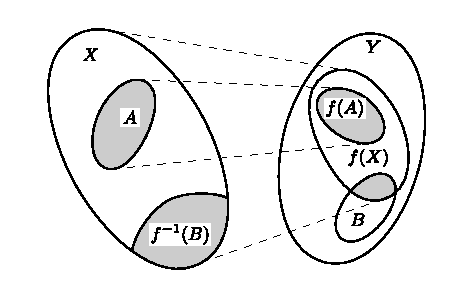
\includegraphics[width=10cm]{attachment/Acr1745354698752707434.pdf}
	\caption{与映射相关的一些集合, 图源Zorich Fig. 1.6}
\end{figure}

\begin{definition}{双射}
	设映射$f: A \to B$.
	\begin{itemize}
		\item 若$A$中的每一个$x$的唯一对应$B$中的一个$f(x)$, 则称$f$是\textit{单射}(injection).
		\item 若对于$B$中的每一个元素$y$, 总能找到$A$中的一个$x$使得$f(x)=y$, 则称$f$是\textit{满射}(surjection).
		\item 若$f$既是单射, 又是满射, 则称$f$是\textit{双射}(bijection)或一一映射.
	\end{itemize}
\end{definition}

\begin{definition}{映射的乘法}
    设映射$f: A \to B$, $g: B \to C$, 则它们的\textit{复合映射}(composite mapping)~$gf: A \to C$定义为$$(gf)(x)=g(f(x)) \ (x \in A).$$
    注意复合运算有先后顺序.容易说明映射$gf$的定义域为$A$, 值域为$C$.
\end{definition}
\begin{remark}
	为了强调复合运算, $gf$也可记作$g \circ f$.
\end{remark}

容易验证, 这样的“乘法”运算满足结合律与分配律、不满足交换律.

一般将$f \circ f \circ \cdots \circ f~(n\textit{次复合})$称作$f$的$n$次迭代\footnote{严格来说, 在获得自然数集的定义之前, 还不能这样写.} , 记作$f^n$.

\begin{definition}{恒等映射}
	设映射$f: A \to A$.称$f$是$A$上的一个\textit{恒等映射}(identity mapping), 如果$$\forall x\in A, ~f(x)=x.$$
	并把$f$记作$\mathcal{I}_A$.
\end{definition}
\begin{remark}
	设映射$f :  A \to B$, 容易验证有$$f\mathcal{I}_A=f, \quad \mathcal{I}_Bf=f.$$
\end{remark}

下面来证明恒等映射是良定义的, 即集合$A$上的所有恒等映射是相等的.假设存在两个不同的恒等映射$\mathcal{I}_1, \mathcal{I}_2$, 那么由$$\mathcal{I}_1 = \mathcal{I}_1 \mathcal{I}_2 = \mathcal{I}_2, $$
可知$\mathcal{I}_1 = \mathcal{I}_2$, 这与假设矛盾.

\begin{definition}{逆映射}
	设映射$f: A \to B$.称$f$是\textit{可逆的}(inverible), 如果存在映射$g: B \to A$满足$$fg=\mathcal{I}_B, \quad gf=\mathcal{I}_A.$$
	特别地, 称$g$为$f$的\textit{逆映射}(inverse mapping).
\end{definition}
\begin{remark}
	必须要求$g$和$f$的两种复合均等于恒等映射. 
\end{remark}

逆映射是唯一的. 实际上, 设映射$g_1, g_2$为$f: A \to B$的不同的逆映射, 那么由$$g_1 = g_1\mathcal{I}_B = g_1fg_2 = \mathcal{I}_Ag_2 = g_2, $$
可知$g_1=g_2$, 这与假设矛盾.

既然一个映射的逆映射是唯一的, 我们可以用符号$f^{-1}$来表示它. 需要区分逆映射与原象集.

下面的命题刻画了何时映射是可逆的.

\begin{proposition}{可逆性等价于双射性}
	设映射$f: A \to B$, 则$f$可逆当且仅当它是双射.
\end{proposition}
\begin{proof}
	(1) 必要性: 设$f$可逆, 即存在映射$g: B \to A$满足$fg=\mathcal{I}_B, gf=\mathcal{I}_A$. 下面证明$f$是双射. 
	
	设$x, y \in A$使得$f(x)=f(y)$, 那么由$x=gf(x)=gf(y)=y$可知$f$是单射. 
	
	另一方面, 设$z \in B$, 由于$z=fg(z)$, 这表明$B \subseteq f(A)$, 故$B = f(A)$, 于是$f$是满射. 
	
	(2) 充分性: 设$f$是单射和满射, 下面证明存在映射$g: B \to A$满足$fg=\mathcal{I}_B, gf=\mathcal{I}_A$. 
	
	人为地取$g$, 使得$g(x)$是$A$中唯一使得$f(g(x))=x$的那个元素(唯一存在性由$f$是双射可以得到保证).按照$g$的定义, 自然有$fg=\mathcal{I}_B$. 
	
	另一方面, 任取$x \in A$, 由于$f(gf(x)) = (fg)(f(x)) = f(x)$并且$f$是单射, 可得$gf(x)=x$, 所以$gf=\mathcal{I}_A$.
\end{proof}

有些函数在定义域上并非是可逆的, 然而利用部分映射可以得到其一部分的逆映射, 例如三角函数.

最后我们来看映射与集合运算的关系: 

\begin{proposition}{映射与集合运算的关系}
	设映射$f:A \to B$, $E_{\alpha}$是$A$的子集, $E'_{\alpha}$是$B$的子集(对任意$\alpha \in I$). 则: 
	$$f \left( \bigcup_{\alpha \in I} E_{\alpha} \right) = \bigcup_{\alpha \in I} f(E_{\alpha});\qquad f \left( \bigcap_{\alpha \in I} E_{\alpha} \right) \subseteq \bigcap_{\alpha \in I} f(E_{\alpha}); $$
	$$f^{-1} \left( \bigcup_{\alpha \in I} E'_{\alpha} \right) = \bigcup_{\alpha \in I} f^{-1}(E'_{\alpha});\qquad f^{-1} \left( \bigcap_{\alpha \in I} E'_{\alpha} \right) = \bigcap_{\alpha \in I} f^{-1}(E'_{\alpha}). $$
\end{proposition}
\begin{remark}
	注意第二个式子的等号不一定能取得. 实际上可以证明, 等号取得当且仅当$f$是单射, 这一结论留作习题. 
\end{remark}
\begin{proof}
	只证明第一个. 一方面, 设$y \in f(\bigcup_{\alpha \in I} E_{\alpha})$, 则存在$\alpha \in I$使得$y \in f(E_{\alpha})$, 那么$f(\bigcup_{\alpha \in I} E_{\alpha}) \subseteq \bigcup_{\alpha \in I} f(E_{\alpha})$. 另一方面是同理的. 由此可得等号成立. 
\end{proof}

\newpage
\section{二元关系}

幂集公理允许我们构造两个集合的Cartesian积.

\begin{definition}{Cartesian积}
	设集合$A$和$B$, 定义它们的\textit{Cartesian积}(Cartesian product,  direct product)如下: $$A \times B : = \{ (a, b): a \in A, b \in B \}.$$
\end{definition}
\begin{remark}
	不难发现Cartesian积是一个可逆的过程, 也即任何一个在$A \times B$中的元素都可以回溯到其在$A$和$B$中的对应元素.因而Cartesian积不满足交换律和结合律.
\end{remark}
\begin{remark}
	特别地, 记$A^2: =A \times A$, 以及$A^n : = A^{n-1} \times A~(n \geq 2)$.
\end{remark}

\begin{definition}{二元关系}
	设非空集合$S$, 则称$S^2$的一个子集$\mathcal{R}$为$S$上的一个\textit{二元关系}(binary relation).若$(a, b) \in \mathcal{R}$, 则称$a, b$有$\mathcal{R}$关系, 记作$a\mathcal{R}b$.
\end{definition}

例如, 对于集合族$M$, 定义在$M$上的关系$$\Delta : = \{ (X, Y) \in M^2 :  \forall x, (x \in X) \Leftrightarrow (x \in Y) \}, $$
那么集合$A, B$相等就可以表述为$A \Delta B$.

\subsection{等价关系}

一类在数学中很重要的关系就是等价关系, 它为我们阐明了数学对象的相似性和一致的本质.

\begin{definition}{等价关系}
	设集合$S$及定义在$S$上的关系$\mathcal{R}$, 如果对任意$a, b, c \in S$都有: 
	\begin{enumerate}
		\item 自反性: $a\mathcal{R} a$; 
		\item 对称性: $a\mathcal{R} b \Rightarrow b\mathcal{R} a$; 
		\item 传递性: $a\mathcal{R} b \wedge b\mathcal{R} c \Rightarrow a\mathcal{R} c$.
	\end{enumerate}
	则称$\mathcal{R}$是$S$上的一个\textit{等价关系}(equivalence relation), 记作$\sim$.
\end{definition}

把所有等价的元素放在一起, 就形成了\textit{等价类}(equivalence class).具体地, 定义$$[a]_{\mathcal{R}} : = \{ x \in S: x\mathcal{R}a \}, $$如果$\mathcal{R}$是$S$上的一个等价关系.

例如, 数论中模$n$的同余关系就是一类等价关系, 而模$n$的同余类就是等价类.

等价类内元素都具有同等地位, 都能代表整个等价类, 否则它们也不会被称作是等价的.

\begin{proposition}{等价类相等等价于代表元素等价}
	设$\mathcal{R}$是$S$上的等价关系, 对于$a, b \in S$有
	\begin{center}
		$[a]_{\mathcal{R}} = [b]_{\mathcal{R}} \Leftrightarrow a\mathcal{R} b.$
	\end{center}
\end{proposition}
\begin{proof}
	必要性显然. 充分性: 任取$c \in [a]_{\mathcal{R}}$, 由传递性知$c \mathcal{R} b$, 所以$c \in [b]_{\mathcal{R}}$, 从而$[a]_{\mathcal{R}} \subseteq [b]_{\mathcal{R}}$.同理有$[b]_{\mathcal{R}} \subseteq [a]_{\mathcal{R}}$, 所以$[a]_{\mathcal{R}} = [b]_{\mathcal{R}}$.
\end{proof}

还是以模$n$的同余类为例. 我们发现, 任何一个整数都会出现且仅会出现在一个同余类里, 换句话说, 所有的同余类构成类对整数集合的划分. 

一般地, 所有的等价类都可以构成对特定集合的划分. 

\begin{definition}{集合的划分}
	对于给定集合$S$, 集合族$X=\{ S_{\alpha} :  \alpha \in I \}$, 其中$I$是指标集.称$X$是$A$的一个\textit{划分}(partition), 如果
	\begin{enumerate}
		\item $S = \bigcup_{\alpha \in I} S_{\alpha}$.
		\item $\forall \alpha \neq \beta , ~S_{\alpha} \cap S_{\beta}$.
	\end{enumerate}
\end{definition}

\begin{theorem}{}
	设$\mathcal{R}$是$S$上的一个等价关系, 则集合族$$\{ [a]_{\mathcal{R}}: a \in S \}$$构成了$S$的一个划分.
\end{theorem}
\begin{proof}
	首先我们证明, 所有$[a]_{\mathcal{R}}$的并集恰等于$S$.注意到$$\forall a \in S, ~a \in [a]_{\mathcal{R}} \wedge [a]_{\mathcal{R}} \subseteq S, $$
	所以$S \subseteq \bigcup_{a \in S} [a]_{\mathcal{R}} \subseteq S$, 从而$S = \bigcup_{a \in S} [a]_{\mathcal{R}}$. 
	
	接着证明这些集合都是不交并. 对于$[a]_{\mathcal{R}} \neq [b]_{\mathcal{R}}$, 假设存在$c \in [a]_{\mathcal{R}} \cap [b]_{\mathcal{R}}$, 那么$c \in [a]_{\mathcal{R}} \wedge c \in [b]_{\mathcal{R}}$, 由等价关系的传递性, $a\mathcal{R}b$, 与假设矛盾. 于是该集合族中任意两个元素交集为空.
\end{proof}

\subsection{序关系}

类比等价关系, 可以定义序关系. 然而就像实数集中的$<$和$\leq$关系一样, 序关系可能有两种形式: 严格的和不严格的. 一般地, 我们更希望使用后者, 例如后面会介绍数列极限运算是维持不严格序关系的. 

容易看出, 上面两种情况的区别在于自反性, 所以只需要把下方定义中的自反性去掉, 就能得到严格偏序关系的定义. 

\begin{definition}{偏序关系}
	设集合$S$及定义在$S$上的关系$\mathcal{R}$, 如果对任意$a, b, c \in S$都有: 
	\begin{enumerate}
		\item 自反性: $a\mathcal{R} a$; 
		\item 反对称性: $a\mathcal{R} b \wedge b\mathcal{R} a \Rightarrow a=b$; 
		\item 传递性: $a\mathcal{R} b \wedge b\mathcal{R} c \Rightarrow a\mathcal{R} c$.
	\end{enumerate}
	则称$\mathcal{R}$是$S$上的一个\textit{偏序关系}(partially ordered relation), 记作$\preceq$.
\end{definition}

为什么偏(partially, 部分地)序关系不直接称作序关系呢? 这是因为, 有些序关系并不能覆盖所有元素. 例如对于给定集合的幂集, 其中某些元素并不存在包含关系. 再例如, 实数间的大小关系就可以覆盖所有元素. 从而引出另一个概念, 全序关系: 

\begin{definition}{全序关系}
	设集合$S$及定义在$S$上的关系$\mathcal{R}$, 如果对任意$a, b, c \in S$都有: 
	\begin{enumerate}
		\item 反对称性: $a\mathcal{R} b \wedge b\mathcal{R} a \Rightarrow a=b$; 
		\item 传递性: $a\mathcal{R} b \wedge b\mathcal{R} c \Rightarrow a\mathcal{R} c$; 
		\item 完全性: $a\mathcal{R} b \vee b\mathcal{R} a$.
	\end{enumerate}
	则称$\mathcal{R}$是$S$上的一个\textit{全序关系}(totally ordered relation), 同时称$S$是一个\textit{全序集}(totally ordered set).
\end{definition}
\begin{remark}
	完全性蕴含了自反性.
\end{remark}

\newpage
\section{集合的基数}

高中数学中, 我们学过有限集合的元素个数. 从直观上看, 似乎无限集合不会存在元素个数这一说法, 但我们又熟知实数远比整数多, 那么这种相对的元素个数比较是怎样建立的? 

来考虑这样一个问题: 给定两个有限集合$A, B$, 如何比较它们的元素个数. 最一般的想法应该是在它们之间构造一个映射$f: A \to B$, 如果$f$是双射则$A, B$元素个数相等, 如果是单射则$A$的元素个数不多于$B$的元素个数, 如果是满射则$B$的元素个数不多于$A$的元素个数(这些用反证法容易说明). 

相对应地, 既然我们只需要考虑无限集合之间的相对“元素个数”多少, 而不需要得到一个绝对数值, 就可以仿照上方的方法定义一个无限集合的“相对元素个数”. 非常直观地, 我们也将其称为“势”, 这是否让你想起电势? 在接下来的内容中, 你将看到集合的“势”的参考位置一般取用自然数集合. 

\begin{definition}{等势集合}
	对于集合$A, B$, 若存在单射$f: A \to B$, 则称$A$的势小于等于$B$, 记作$|A| \leq |B|$.特别地, 若单射$f$同时也是一个满射, 即$f$是双射, 则称$A, B$\textit{等势}(equipollent), 记作$|A|=|B|$.
\end{definition}

很自然地, 我们可以证明集合的等势关系是一个等价关系. 为了证明势的小于等于是一个全序关系, 需要下方的定理: (解决这个定理需要一个巧妙的构造, 初学者只需学习证明的严格性即可)

\begin{theorem}{Schröder–Bernstein}
	给定集合$A, B$.若在$A, B$间存在两个单射$f: A \to B$与$g: B \to A$, 则在它们之间也存在一个双射$h: A \to B$.
\end{theorem}
\begin{proof}
	通过以下方法构造一个映射$h: A \to B$, 我们断言它就是想要的那个双射. 
	
	递归地定义: $$C_0 = A - g(B), \quad C_{n+1}=g(f(C_n))~~\forall n \geq 0.$$
	并记$C = \bigcup_{n=0}^{\infty} C_n$.对任意的$x \in A$定义映射$h:  A\to B$满足$$h(x) = \begin{cases}
 f(x) &  x \in C \\
 g^{-1}(x) &  x \notin C
\end{cases}, $$并注意这里$g$的逆映射定义域被限制在了$g(B)$. 由$C_0$的定义可知, 若$x \notin C$, 则$x \in g(B)$, 所以这样的限制是合理的. 接下来验证$h$是双射. 

(1) 单射性: 假设不同的$a, b$导致$h(a)=h(b)$, 对以下四种情况进行讨论: $$a \in C \wedge b \in C, \qquad a \notin C \wedge b \notin C, \qquad a \in C \wedge b \notin C, \qquad a \notin C \wedge b \in C.$$
对于前两种情况, 容易证明$a=b$.对于第三种情况, 即有$g(f(a))=b$, 而$a \in C$表明$g(f(a)) \in C$, 从而与$b \notin C$矛盾.第四种情况同理. 

综上, 对任意$a, b$都有$h(a)=h(b) \Rightarrow a=b$, 故$h$是单射. 

(2) 满射性: 任取$y \in B$. 若$y \in f(A)$, 则存在一个$x_1$使得$f(x_1)=y$, 从而$h(x_1)=y$. 若不然, 则令$x_2=g(y)$.下面证明$x_2 \notin C$, 这样就有$h(x_2)=g^{-1}(x_2)=y$: 

假设$x_2=g(y) \in C$, 那么由$C$的定义且$g$为单射, 可知存在一个$x_0$使得$f(x_0)=y$, 这与$y \notin f(A)$矛盾. 

综上, 对任意的$y \in B$, 总能找到某个$x$使得$h(x)=y$, 从而$h$是满射.
\end{proof}

由上方的定理, 容易得到势的小于等于关系满足反对称性. 该关系的完全性是选择公理的推论(这里略去). 再加上传递性(例如, $A, B$之间存在单射$f$, $B, C$之间存在单射$g$, 则$g|_{f(A)} \circ f$是$A, C$间的单射), 马上得到该关系是一个全序关系. 

从而, 我们可以利用等价类的思想刻画一个无限集合的相对元素个数.

\begin{definition}{集合的基数}
	\vspace{-2em}
	\begin{itemize}
		\item 设集合的等势关系$\mathcal{R}$.对于集合$X$, 称$[X]_{\mathcal{R}}$为其\textit{基数}(cardinal)或势, 记作$\card X$.
		\item 定义$\card X = \card Y$, 如果$X$与$Y$等势.
		\item 定义$\card X \leq \card Y$, 如果$X$与$Y$的某个子集等势.
	\end{itemize}
\end{definition}

容易证明集合基数的小于等于关系也是一个全序关系.

关于无限集合, Cantor曾证明: (这里$(\card X < \card Y): = (\card X \leq \card Y) \wedge (\card X \neq \card Y)$.)

\begin{theorem}{}
	设集合$X$, 则$\card X < \card \mathcal{P}(X)$.
\end{theorem}
\begin{proof}
	若$X$是空集, 则显然成立.从而, 只考虑$X$非空的情况. 
	
	由于$\mathcal{P}(X)$涵盖所有$X$的一元子集, 故显然有$\card X \leq \card \mathcal{P}(X)$. 假设有$\card X = \card \mathcal{P}(X)$, 那么存在双射$f: X \to X$. 
	
	根据$f$, 取$B=\{ x \in X: x \notin f(x) \}$, 显然$B \in \mathcal{P}(A)$, 从而存在$x$使得$f(x)=B$. 此时, 若$x \in B$, 则由$B$的定义知$x \notin B$, 矛盾; 同理, 若$x \notin B$, 则可得$x \in B$, 也矛盾. 
\end{proof}
\begin{remark}
	本定理亦可使用Cantor对角线法证明, 请参考下一章的部分内容. 
\end{remark}

\newpage
\section*{一些习题 ~~\small 对应原书第一章习题} \label{sec:ex1.1}

\subsection*{A: 映射与集合运算的关系}

设$f:X \to Y$, $A,B$是$X$的任意子集, $A',B'$是$Y$的任意子集. 
\vspace{1em}

\circled{A1}-1~~证明: 
\begin{center}
	a) $(A \subset B) \Rightarrow (f(A) \subset f(B)) \nRightarrow (A \subset B)$,\qquad b) $(A \neq \varnothing) \Rightarrow (f(A) \neq \varnothing)$,
	
	c) $f(A \cap B) \subset f(A) \cap f(B)$,\qquad d) $f(A \cup B) = f(A) \cup f(B)$.
\end{center}

\circled{A1}-2~~证明: 
\begin{center}
	a) $(A' \subset B') \Rightarrow (f^{-1}(A') \subset f^{-1}(B'))$,\qquad b) $f^{-1}(A' \cap B') = f^{-1}(A') \cap f^{-1}(B')$,
	
	c) $f^{-1}(A' \cup B') = f^{-1}(A') \cup f^{-1}(B')$.
\end{center}
	
\circled{A1}-3~~证明: 
\begin{center}
	a) $f^{-1}(A'-B') = f^{-1}(A') - f^{-1}(B')$,\qquad b) $f^{-1}(Y-A') = X-f^{-1}(A')$.
\end{center} 

\circled{A1}-4~~证明: 
\begin{center}
	a) $f^{-1}(f(A)) \supset A$,\qquad b) $f(f^{-1}(B')) \subset B'$.
\end{center} 
\vspace{1em}

\circled{A2}~~证明下列命题是等价的: 

\begin{center}
	a) $f$是单射; \qquad b) $f^{-1}(f(A))=A$; \qquad c) $f(A \cap B) = f(A) \cap f(B)$;
	
	d) $f(A) \cap f(B) = \varnothing \Leftrightarrow A \cap B = \varnothing$; \qquad e) $f(A-B) = f(A) - f(B)$, 其中$B \subseteq A$. 
\end{center}
\vspace{1em}

\subsection*{B: 一些集合论的补充}

\circled{B1}~~分别利用Schröder–Bernstein和直接构造双射证明: $[0,1]$和$(0,1)$是等势的. 
\vspace{1em}


\circled{B2}~~使用集合论公理证明von Neumann构造的自然数集$\mathbb{N}_0$中的元素满足如下性质: 
	\begin{center}
		i) $x=y \Rightarrow x^+ = y^+$; \qquad ii) $\forall x \in \mathbb{N}_0,~x^+ \neq \varnothing$;
	
		iii) $(A \subseteq \mathbb{N}_0) \wedge (\varnothing \in A) \wedge (\forall x \in A,~x^+ \in A) \Rightarrow A=\mathbb{N}_0$; \qquad iv) $x^+=y^+ \Rightarrow x=y$.
	\end{center}


\chapter{实数理论}

\section{自然数集的构造与公理化}

回顾第一章的练习1.5 a), 如果将$x \mapsto x^+$的过程视作后继映射$S: N_0 \to N_0$, 我们在von Neumann构造的自然数集中实际上证明了以下四件事情: 

i) $x=y \Rightarrow x^+ = y^+$, 即该映射的定义是合理的; 

ii) $\forall x \in N_0, ~x^+ \neq \varnothing$, 即$\varnothing \notin S(N_0)$; 

iii) $(A \subseteq N_0) \wedge (\varnothing \in A) \wedge (\forall x \in A, ~x^+ \in A) \Rightarrow A=N_0$, 即如果自然数集的子集也是归纳集, 那么该子集就是自然数集本身; 

iv) $x^+=y^+ \Rightarrow x=y$, 即$S$是一个单射.

以上四件事情在熟知的那个自然数集中似乎也是成立的. 那么, 能否将所有具有如上性质的集合都考虑为自然数集呢? 具体地讲, 我们需要一些公理.

\begin{axiom}{Peano公理}
	设集合$X$及其上的一个映射$S$. 若$X$和$S$满足
	\begin{enumerate}
		\item $x \in X$; 
		\item $x \notin S(X)$; 
		\item $S$是一个单射; 
		\item $X$对于$S$是封闭的; 
		\item (极小性公设)对任意$A \subseteq X$都有: 若$x \in A$且$A$对$S$封闭, 则$A=X$. 
	\end{enumerate}
	则$X$是自然数集. 
\end{axiom}
\begin{remark}
	一般称$x$为初始元素, $S$为后继映射. 由$(X, S, x)$构成的组称为一个Peano系统. 一般记$0: =x$.
\end{remark}

如果第二条不成立, 可能会存在某个元素的后继为初始元素, 从而形成循环; 如果第三条不成立, 则有可能两个元素的后继是同样的; 若第四条不成立, 则会有某个元素后面没有后继元素; 第五条也被称为归纳原理, 用处在于排除多链的情况. 

\begin{figure}[h!]
	\centering
	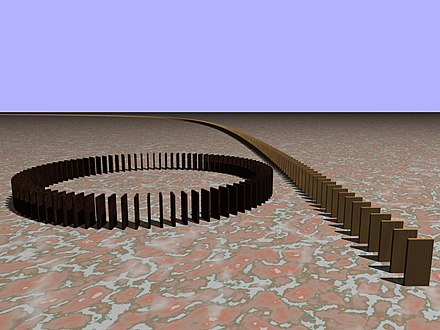
\includegraphics[width=6cm]{attachment/440px-Domino_effect_visualizing_exclusion_of_junk_term_by_induction_axiom.jpg}
	\caption{多链示意图, 深色的骨牌是我们不想要的. 图源Wikipedia}
\end{figure}



1.5 a)的四条结论和$N_0$的定义足以说明$N_0=\mathbb{N}$.也即, 通过定义$\mathbb{N}$是最小的归纳集和利用Peano公理定义$\mathbb{N}$是完全等价的.

定义前10个自然数的符号分别为$0, 1, 2, 3, 4, 5, 6, 7, 8, 9$.

这里再声明一次(第一)数学归纳法, 方便后面使用.

\begin{theorem}{第一数学归纳法} \label{thm:diyigvna}
	设$P(n)$是关于自然数$n$的一个性质. 如果
	\begin{enumerate}
		\item 当$n=0$时, $P(n)$成立; 
		\item 由$P(n)$成立可以推出$P(n+1)$成立.
	\end{enumerate}
	那么, 对任意$n \in \mathbb{N}$, $P(n)$都成立.
\end{theorem}
\begin{proof}
	这是极小性公设的直接推论. 
\end{proof}

\subsection{自然数集上的加法}

自然数中可以一步完成的加法已经有明确的定义: $n+0=n, ~n+1=S(n)$.从而可以归纳地定义完全的加法.

\begin{definition}{自然数集上的加法}
	设自然数集$\mathbb{N}$, $S$是$\mathbb{N}$上的后继映射.定义自然数集上的\textit{加法}(addition)映射为满足如下条件的映射$+: \mathbb{N}^2 \to \mathbb{N}, ~(n, m) \to n+m$: 
	\begin{enumerate}
		\item $n+0=n$.
		\item $n+S(m)=S(n+m)$.
	\end{enumerate}
\end{definition}

既然加法是归纳定义, 我们同样可以利用归纳法证明加法的诸多性质: (证明略去, 后文亦如此)

\begin{proposition}{自然数的加法运算律}
	对于任意的$a, b, c \in \mathbb{N}$, 都有
	\begin{enumerate}
		\item (结合律)~$(a+b)+c = a+(b+c)$.
		\item (交换律)~$a+b=b+a$.
		\item (消去律)~$a+c=b+c \Leftrightarrow a=b$.
	\end{enumerate}
\end{proposition}

为了得到熟悉的减法定义与运算律, 要先明确构造的可行性: (其中$\mathbb{N}^* : = \mathbb{N} - \{ 0 \}$.)

\begin{proposition}{} \label{pro:jmfagzzckexkxk}
	对任意$b \in \mathbb{N}^*$, 存在$a \in \mathbb{N}$使得$S(a)=b$.
\end{proposition}

\subsection{自然数集中的序关系}

类似于利用$a=kb$定义$b \mid a$这一序关系, 可以利用加法来定义自然数的序关系.

\begin{definition}{自然数集中的序关系}
	设$a, b \in \mathbb{N}$.如果存在$k \in \mathbb{N}$使得$a+k=b$, 则称$a$\textit{小于等于}(less than or equal to)$b$, 记作$a \leq b$.特别地, 若$a \leq b$且$a \neq b$, 则称$a$\textit{小于}(less than), 记作$a<b$.
\end{definition}

自然数集中的小于等于关系是一个全序关系, 利用归纳法容易验证其满足传递性、反对称性、完全性.

关于小于关系, 还有一个类似完全性的命题: 

\begin{proposition}{自然数集的三歧性}
	对于任意$a, b \in \mathbb{N}$, 下列命题中恰有一个成立: 
	\begin{center}
		$a<b,  \qquad a=b,  \qquad a>b.$
	\end{center}
\end{proposition}


\begin{proposition}{自然数的加法保序性}
	对于任意$a, b, c \in \mathbb{N}$, 有
	\begin{center}
		$a+c \geq b+c \Leftrightarrow a \geq b.$
	\end{center}
\end{proposition}

自然数还有一项重要的性质: 

\begin{proposition}{自然数的离散性}
	对于任意$a, b \in \mathbb{N}$都有
	\begin{center}
		$a>b \Leftrightarrow a \geq S(b).$
	\end{center}
\end{proposition}

现在, 我们对数学归纳法做一些集中的研究.

\begin{theorem}{第二数学归纳法} \label{thm:diergvna}
	设$P(n)$是关于自然数$n$的一个性质.如果
	\begin{enumerate}
		\item 当$n=0$时, $P$成立; 
		\item 假设$n \leq k$时$P(n)$都成立, 则当$P(k+1)$也成立.
	\end{enumerate}
	那么, 对任意$n \in \mathbb{N}$, $P(n)$都成立.
\end{theorem}

\begin{theorem}{良序定理} \label{thm:llxu}
	对于任意非空集合$A \subseteq \mathbb{N}$, $A$中都存在一个元素$M$, 使得$\forall a \in A, ~a \geq M$.
\end{theorem}
\begin{proof}
	假设对任意的$M$, 总存在某个$a \in A$使得$a < M$. 下面归纳证明$A^c = \mathbb{N}$. 
	
	(i)假设$0 \in A$, 又由于任意自然数$n$有$n \geq 0$(利用命题\ref{pro:jmfagzzckexkxk}结合归纳法可以证明), 于是与$A$的定义矛盾, 故$0 \notin A$, 那么$0 \in A^c$. 
	
	(ii)假设对任意的$n \leq k$, 都有$n \in A^c$即$n \notin A$, 那么假若$k+1 \in A$, 由于$n \leq k < k+1$, 这与$A$的定义矛盾, 所以$k+1 \notin A$, 从而$k+1 \in A^c$. 
	
	由第二数学归纳法可知, $A^c = \mathbb{N}$, 即$A = \varnothing$, 与假设矛盾. 所以原命题成立.
\end{proof}

反过来, 利用反证法也能说明良序定理可以推导第一数学归纳法.从而, 定理\ref{thm:diyigvna}, \ref{thm:diergvna}, \ref{thm:llxu}是等价的.

\subsection{自然数集中的乘法}

仿照加法, 继续归纳定义乘法: 

\begin{definition}{自然数集上的乘法}
	设自然数集$\mathbb{N}$, $S$是$\mathbb{N}$上的后继映射. 定义自然数集上的\textit{乘法}(multiplication)映射为满足如下条件的映射$\times : \mathbb{N}^2 \to \mathbb{N}, ~(n, m) \to n \times m$: 
	\begin{enumerate}
		\item $n\times 0=0$.
		\item $n\times S(m)=n\times m+n$.
	\end{enumerate}
\end{definition}

如此定义的乘法和我们心中的模样如出一辙: 利用归纳法容易证明$n \times m = \overbrace{n+n+\cdots +n}^{m~ \text{times}}$. 在获得乘法交换律之前, 注意$m$和$n$的顺序! 

利用归纳法, 不难证明下列命题: 

\begin{proposition}{自然数的乘法运算性质}
	对于任意的$a, b, c \in \mathbb{N}$, 都有
	\begin{enumerate}
		\item (分配律)~$(a+b)c = ab+ac$.
		\item (单位元)~$a \times 0 = 0 \times a = 0, ~a \times 1 = 1 \times n = n$.
		\item (交换律)~$ab=ba$.
		\item (结合律)~$(ab)c=a(bc)$.
	\end{enumerate}
\end{proposition}

为了得到消去律, 还要再做些准备: 

\begin{proposition}{自然数的乘法无零因子律}
	对任意$a, b \in \mathbb{N}$, $ab=0$当且仅当$a=0$或$b=0$.
\end{proposition}

\begin{proposition}{自然数的乘法保序性}
	对于任意$a, b, c \in \mathbb{N}$, 其中$c \neq 0$, 总有
	\begin{center}
		$a>b \Leftrightarrow ac>bc.$
	\end{center}
\end{proposition}

结合乘法保序性, 利用反证法可以得到乘法消去律.

\begin{corollary}{自然数的乘法消去律}
	对于任意$a, b, c \in \mathbb{N}$, 其中$c \neq 0$, 总有
	\begin{center}
		$a=b \Leftrightarrow ac=bc.$
	\end{center}
\end{corollary}

乘法是对加法的累积, 次幂则是对乘法的累积.

\begin{definition}{自然数的次幂}
	设自然数集$\mathbb{N}$, $S$是$\mathbb{N}$上的后继映射.定义自然数集上的\textit{指数}(exponentiation)映射为满足如下条件的映射$\sigma : \mathbb{N}^2-\{ (0, 0) \} \to \mathbb{N}, ~(n, m) \to n^m$: 
	\begin{enumerate}
		\item 对于$n \neq 0$, 有$n^0=1$, $n^{S(m)}=n^m \times n$.
		\item 对于$n \neq 0$, 若$m \neq 0$则$n^m=0$.
	\end{enumerate}
\end{definition}

同样利用归纳法可以证明, $n^m = \overbrace{n\times n\times \cdots \times n}^{m~ \text{times}}$.


\newpage
\section{整数环的构造}

在自然数集中定义减法时, 我们会注意到, 并不是所有自然数相减都会得到自然数, 也即自然数集对加法逆元不封闭. 为了保证封闭, 尝试在自然数的基础上构造整数.

通过自然数的差来构造整数是一个好思路. 不过, 这种相对差量不能保证唯一性, 即整数$a$可能通过任意的$(a+k)-k$得到. 从而, 可以考虑用等价类的方法定义整数. 

\begin{definition}{整数集}
	在$\mathbb{N}^2$上定义等价关系$\sim$如下: $$(a_1, b_1) \sim (a_2, b_2) : \Leftrightarrow a_1+b_2=a_2+b_1.$$
	将每个等价类视作一个\textit{整数}(integer), 所有等价类构成的集合视作整数集, 记作$\mathbb{Z}$.
\end{definition}

接着定义整数集里的加法与乘法: 

\begin{definition}{整数集的加法和乘法}
	规定加法: $$[(a_1, b_1)]_{\sim} + [(a_2, b_2)]_{\sim} : = [(a_1+b_1, b_1+b_2)]_{\sim}.$$
	乘法: 
	$$[(a_1, b_1)]_{\sim} \times [(a_2, b_2)]_{\sim} : = [(a_1a_2+b_1b_2, a_1b_2+a_2b_1)]_{\sim}.$$
\end{definition}

如此定义的加法和乘法显然是良定义的. 

接着可以得到理想中的结果: 上述定义的整数集同构于自然数集的某个母集. 或者反过来更好描述: 自然数集同构(存在双射并保持代数结构)于整数集的某个子集. 

\begin{proposition}{}
	记$\tilde{\mathbb{N}}: =\{ [(a, b)]_{\sim} \in \mathbb{Z}: a \leq b \}$.那么存在双射$$\sigma : \tilde{\mathbb{N}} \to \mathbb{N}, ~[(a, b)]_{\sim} \mapsto a-b, $$
	并且有$$\sigma (\alpha) + \sigma (\beta) = \sigma (\alpha + \beta), \quad \sigma (\alpha) \times \sigma (\beta) = \sigma (\alpha  \beta)$$
	对于所有$\alpha , \beta \in \tilde{\mathbb{N}}$成立.
\end{proposition}

大一统的基业既已完成, 我们终于得以见到熟悉的记号了: 

\begin{definition}{}
	对于$[a, b]_{\sim} \in \mathbb{Z}$, 由自然数的三歧性可知$a>b, a=b$或$a<b$. 
	\begin{itemize}
		\item 当$a>b$时, 记$n: =[(a, b)]_{\sim}$, 其中$n$是满足$a=b+n$的自然数, 此时称$n$为\textit{正的}(positive). 
		\item 当$a<b$时, 记$-n: =[(a, b)]_{\sim}$, 其中$n$是满足$b=a+n$的自然数, 此时称$-n$为\textit{负的}(negative). 
		\item 当$a=b$时, 记$0: =[(a, b)]_{\sim}$, 这里$0$是自然数集的最小元素.
	\end{itemize}
\end{definition}

将自然数集的一些性质推广, 容易得到: 

\begin{proposition}{整数运算的性质}
	(1) 单位元$$\forall a \in \Z ,  a + 0 = 0+ a = a ,  1 a = a 1 = a .$$
	(2) 加法逆元$$\forall a \in \Z ,  \exists ! b \in \Z ,  a + b = 0 .$$
	(3) 结合性质$$\forall a ,  b ,  c \in \Z ,  (a + b) + c = a + (b + c) ,  (a b) c = a (b c) .$$
	(4) 交换性质$$\forall a ,  b \in \Z ,  a + b = b + a ,  a b = b a .$$
	(5) 分配性质$$\forall c ,  a ,  b \in \Z ,  c (a + b) = c a + c b, (a+b)c=ac+bc .$$
\end{proposition}

\begin{proposition}{整数的乘法无零因子律}
	对任意$a, b \in \Z$, $ab=0$当且仅当$a=0$或$b=0$.
\end{proposition}

\begin{corollary}{整数的乘法消去律}
	对于任意$a, b, c \in \Z$, 其中$c \neq 0$, 总有$$a=b \Leftrightarrow ac=bc.$$
\end{corollary}

实际上, 如果集合$G$上的一个运算$\bigcdot$满足单位元、逆元、结合性质, 我们就称$(G,\bigcdot )$是一个\textit{群}(group). 如果$\bigcdot$还满足交换性质, 则称$(G,\bigcdot )$是一个\textit{交换群}(commutative group)或\textit{Abel群}(Abel group).

在一个集合上, 往往只定义了加法, 例如平面向量(因为平面向量之间的内积和外积都不封闭). 有些时候可以得到具有加法和乘法的集合, 例如所有映射构成的集合, 但是它们的乘法不满足交换性质. 

对于定义了加法和乘法的集合, 可以得到所谓环的概念: 

\begin{axiom}{环}
	设非空集合$R$, 若$R$上定义了加法$+$和乘法$\bigcdot$并满足: 
	\begin{enumerate}
		\item $(R,+)$构成Abel群; 
		\item $\bigcdot$满足结合性质; 
		\item $\bigcdot$对$+$有分配性质. 
	\end{enumerate}
	则称$(R,+,\bigcdot )$是一个\textit{环}(ring).
\end{axiom}

整数集$(\Z ,+,\times )$显然是一个环. 由两个集合间所有映射构成的集合也是一个环. 

考虑一整个代数结构而不是单纯的特例, 可以方便我们迁移应用. 例如, 整数环与一元多项式环的性质非常相似, 所以它们共享很多定理与定义(带余除法定理, 素数和既约多项式等等). 

\begin{definition}{整数的减法}
	记$-n$表示整数$n$的加法逆元.则定义减法映射$-: \Z ^2 \to \Z , (a, b) \mapsto a-b$, 满足$$a-b: =a+(-b).$$
\end{definition}

良定义是显然的.

\begin{definition}{整数的序关系}
	对于$[(a_1, b_1)]_{\sim}, [(a_2, b_2)]_{\sim} \in \Z$, 定义它们的序关系: $$[(a_1, b_1)]_{\sim} \leq [(a_2, b_2)]_{\sim} \Leftrightarrow a_1+b_2 \leq b_1+a_2.$$
\end{definition}

注意$n$为负就等价于$n<0$.

容易验证, 整数间的序关系是一个全序关系, 并且自然数的三歧性在这里同样使用.

整数间的序关系比较复杂, 例如对于负数$c$, $a \leq b \Leftrightarrow ac \geq bc$. 这些熟知性质就不一一罗列了.

\newpage
\section{有理数域的构造}

从自然数集扩大得到的整数集虽然对减法封闭了, 它对除法还是不封闭. 用同样的方式可以将整数集扩大到有理数集.

\begin{definition}{有理数集}
	在$\mathbb{Z}^2$上定义等价关系$\sim$如下: $$(a_1, b_1) \sim (a_2, b_2) : \Leftrightarrow a_1b_2=a_2b_1.$$
	将每个等价类$[(a, b)]_{\sim}$视作一个\textit{有理数}(rational number), 记作$a/b$. 所有等价类构成的集合视作有理数集, 记作$\mathbb{Q}$.
\end{definition}

由定义可知, $(a, b)\in a/b$等价于$(ka, kb) \in a/b$, 这里$k$为任意非零整数. 

\begin{definition}{有理数集的加法和乘法}
	规定加法: $$\frac{a_1}{b_1} + \frac{a_2}{b_2} = \frac{a_1b_2+a_2b_1}{b_1b_2}.$$
	乘法: 
	$$\frac{a_1}{b_1} \times \frac{a_2}{b_2} = \frac{a_1a_2}{b_1b_2}.$$
\end{definition}

只需注意到, $\mathbb{Q}$中的加法单位元为$0/1$, 乘法单位元为$1/1$, 容易验证$(\mathbb{Q}, + ,\times )$也是一个环, 并且乘法满足单位元、逆元、交换性质.

类似地, 可以将$\Z$与$\mathbb{Q}$中的某个子集同构. (这里$b \mid a, ~a, b \in \Z$表示存在$n \in \Z$使得$a=nb$.)

\begin{proposition}{}
	记$\tilde{\mathbb{Z}}: =\{ a/b \in \mathbb{Q}: b \mid a \}$.那么存在双射$$\sigma : \tilde{\mathbb{Z}} \to \mathbb{Q}, a/b \mapsto n, $$
	并且有$$\sigma (\alpha) + \sigma (\beta) = \sigma (\alpha + \beta), \quad \sigma (\alpha) \times \sigma (\beta) = \sigma (\alpha  \beta)$$
	对于所有$\alpha , \beta \in \tilde{\mathbb{Z}}$成立.
\end{proposition}

有理数的除法正如我们在小学学过的那样: 

\begin{definition}{有理数的除法}
	记$a^{-1}$表示有理数$a\neq 0$的乘法逆元.则定义除法映射$\div : \mathbb{Q} ^2 \to \mathbb{Q} , (a, b) \mapsto a \div b$, 满足$$a \div b: =a\times b^{-1}.$$
\end{definition}

良定义是显然的.

从有理数集可以抽象出域公理: 

\begin{axiom}{域}
	设非空集合$F$, 若$F$上定义了加法$+$和乘法$\bigcdot$并满足: 
	\begin{enumerate}
		\item $(F,+,\bigcdot)$是一个环; 
		\item $\bigcdot$满足单位元、逆元、交换性质.
	\end{enumerate}
	则称$F$是一个\textit{域}(field).
\end{axiom}

有理数集是一个域.

由乘法逆元可得消去律和无零因子律: 

\begin{proposition}{域的乘法消去律}
	对于任意$a, b, c \in F$, 其中$c \neq 0$, 总有
	\begin{center}
		$a=b \Leftrightarrow ac=bc.$
	\end{center}
\end{proposition}

\begin{corollary}{域的乘法无零因子律}
	对任意$a, b \in F$, $ab=0$当且仅当$a=0$或$b=0$.
\end{corollary}

在规定有理数的序关系之前, 先明确它与$0$的大小比较. 对于$a/b \in \mathbb{Q}$, 称其为\textit{正的}(positive), 如果$a, b$均为正或均为负; 称其为\textit{负的}(negative), 如果$a, b$一正一负. 

\begin{definition}{有理数的序关系}
	对于$p=a_1/b_1, q=a_2/b_2 \in \mathbb{Q}$, 定义它们的序关系: 在$p, q$一非负一非正时, 不妨设$p$非负, 则$q \leq p$. 在$p, q$均为正或均为负时, 
	$$p \leq q \Leftrightarrow \begin{cases}
		a_1b_2 \leq a_2b_1 & \textit{如果$p, q$均为正} \\
		a_2b_1 \geq a_1b_2 & \textit{如果$p, q$均为负}
	\end{cases}.$$
\end{definition}

可以验证, 有理数$p$为正等价于$p>0$. 有理数的序关系也是一个全序关系, 且满足三歧性.

有理数的序关系也满足整数序关系的那些性质, 这里省略.

\begin{theorem}{Archimedes性质}
	对于给定的正数$n$和任意的有理数$x$, 存在唯一一个整数$k$使得
	\begin{center}
		$kn \leq x < (k+1)n.$
	\end{center}
\end{theorem}
\begin{proof}
	不妨考虑$x>0$和$n=1$. 记$x=p/q$, 用$q$对$p$作带余除法, 设$p=kq+r$, 其中$0 \leq r <q$. 容易验证$k-1 \leq x < k$. 
	
	下证唯一性. 假设整数$\ell \neq k$同样满足$(\ell -1) \leq x < \ell$. 不妨设$\ell >k$, 但是$\ell \geq k+1$, 那么$x \geq \ell \geq k+1 >x$, 矛盾. 
\end{proof}

在定义完实数之后, 利用实数的完备性可以证明Archimedes性质对所有实数$x$也成立. 所以, 尽管Archimedes性质有许多好用的推论, 我们选择在实数部分再介绍. 

\newpage
\section{实数的构造}

实数究竟是什么? 

中学课本说它就是有理数和无理数的总和, 但是也定义无理数是“不是有理数的数”, 这样的概念还是过于无力了: 为什么复数集不能是实数集? 

一方面, 从序关系的角度看, 复数不能排序, 所以实数集至少需要是一个全序集. 另外, 有理数通过代数运算可以得到无理数(例如$\sqrt{2}$), 无理数也能参与有理数的排序, 这说明有理数不够大. 所以, 我们想要找到一个\textit{比有理数集更加“完备”的全序集}作为实数集. 

另一方面, 从图像的角度来看, 复数并不能在数轴上出现, 而有理数并不能覆盖整个数轴. 这样就产生了定义实数的另一个想法: \textit{与数轴上的点一一对应的集合}.但这种定义也存在问题: 数轴是什么? 点是什么? 避开这些抽象的概念, 利用数轴的最本质特征就可以定义实数: 数轴是\textit{连续不断}的一条直线. 所以我们希望实数满足\textit{连续不断}这一特质. 

最后, 考虑十进制小数. 熟知有理数表示为十进制小数时总会是有限的或得到某些循环(这是数论里的一个定理), 而无理数均无法表示为有限小数或可循环的无限小数. 截取无理数的小数点后任意长度的数字, 总是能找到与这段数字相等的有理数. 这意味着考虑实数(特别是无理数)时需要用到\textit{利用有理数进行逼近}的思想. 

实际上, 上文提到的几种思考角度, 分别对应实数的完备性(连续性)和实数构造的特点.

我们首先通过Dedekind分割逼近地定义实数.

\subsection{Dedekind分割}

在数轴上抓住一个点进行研究.先以无理数为例, 我们发现, 比它小的有理数集合总是没有上界, 而比它大的有理数集合总是没有下界.另外, 这两个集合可以构成有理数集的一个划分.我们可以把一个划分一一对应为一个无理数.

但是对于有理数, 上述的两个有理数集合之并集就不能达到有理数集了.稍微修改一下, 我们只需要将上集的定义从“大于”改为“不小于”, 依然可以唯一确定有理数.

还有一件事情要注意: 并不是有理数集合的所有划分都能满足上述的理想状态, 我们需要排除掉多个区间进行划分的情况.因此, 可以规定这两个集合是“接连不断的”. (实际上只用规定一个就够了, 因为划分会强制让另一个集合也接连不断)

总结这些内容, 就是所谓Dedekind分割的基本思想: 

\begin{definition}{Dedekind分割}
	设$\alpha , \beta$构成全序数集$K$的一个划分.若满足
	\begin{enumerate}
		\item $\forall x, y \in K, ((x < y) \wedge (y \in \alpha)) \Rightarrow x \in \alpha$.
		\item $\forall x \in \alpha , \exists y \in \alpha (y>x)$.
	\end{enumerate}
	则称$\alpha$和$\beta$构成$K$的一个\textit{Dedekind分割}(Dedekind cut), 记作$\alpha \mid \beta$. 
\end{definition}

上述定义主要着眼于下集$\alpha$, 所以考虑用下集定义实数: 

\begin{definition}{}
	有理数域上Dedekind分割得到的每个下集称作一个\textit{实数}(real number), 所有下集构成的集合称作实数集.
\end{definition}

最后, 我们来看一个稍有技术性的例子, 这会帮助我们认识有理数域的缺陷. 

\begin{example}
	设集合$$\alpha = \{ a \in \Q :a^2 < 2 \},\qquad \beta = \{ a \in \Q :a^2>2 \}. $$
	则$\alpha$中无最大元素, $\beta$中无最小元素. 
\end{example}
\begin{proof}
	设$f(a)=\frac{2a+2}{a+2}$, 容易验证$$f(a)-a = \frac{2-a^2}{a+2},\quad (f(a))^2-2 = \frac{2(a^2-2)}{(a+2)^2}. $$
	不妨$a>0$. 若$a \in \alpha$, 则$f(a) \in \alpha$, 但是$f(a) > a$; 若$a \in \beta$, 则$f(a) \in \beta$, 但是$f(a) < a$. 
\end{proof}
\begin{remark}
	解答中给出的看似精妙的构造实际上利用了压缩映射原理. 
\end{remark}

\subsection{实数集上的序结构和代数结构}

\begin{definition}{实数集上的序关系}
	设$\alpha , \beta \in \R$.称$\alpha \leq \beta$, 如果$\alpha \subseteq \beta$.
\end{definition}

容易验证, 虽然集合的包含关系并不是全序关系, 但在Dedekind分割的限制下可以做到全序. 亦可证明, 实数的序关系满足三歧性. 

\begin{definition}{实数集上的加法}
	定义$+: \R ^2 \to \R , (\alpha , \beta) \mapsto \alpha + \beta$, 满足
	\begin{center}
		$\alpha + \beta = \{ a+b: a \in \alpha , b \in \beta \}.$
	\end{center}
\end{definition}

亦可验证, 加法是良定义的. 

\begin{proposition}{实数集上加法的运算律}
	实数集上的加法满足:  \\
	(1)结合性质: 
	\begin{center}
		$\forall \alpha , \beta , \gamma \in \R , ~(\alpha + \beta ) + \gamma = \alpha + (\beta + \gamma).$
	\end{center}
	(2)交换性质: 
	\begin{center}
		$\forall \alpha , \beta \in \R, ~\alpha + \beta = \beta + \alpha .$
	\end{center}
	(3)单位元: 
	\begin{center}
		$\exists ! 0 \in \R , ~\forall \alpha \in \R ,  \alpha + 0 = 0 + \alpha = \alpha .$
	\end{center}
	(4)逆元: 
	\begin{center}
		$\forall \alpha \in \R , ~\exists ! \beta \in \R , ~\alpha + \beta = \beta + \alpha = 0.$
	\end{center}
\end{proposition}
\begin{proof}
	只证明(3)和(4).注意这里的$0$并非自然数$0$, 而是某个下集. 
	
	(3) 单位元的唯一性可类比于整数单位元证明.下面构造地证明单位元的存在性: 声明$0 : = \mathbb{Q}_{-} \in \R$.任取$\alpha \in \R$, 下面证明$\alpha + 0 = \alpha$:  
	
	(i) 任取$a \in \alpha , b \in 0$, 因为$a + b < a$, 所以$\alpha + 0 \subseteq \alpha$. 
	
	(ii) 任取$a \in \alpha$.由定义知存在$a'>a$使得$a' \in \alpha$.记$x=a-a'<0$, 所以$x \in 0$.从而$\alpha \subseteq \alpha + 0$. 
	
	综上可得, $\alpha +0 = \alpha$. 
	
	(4) 逆元的唯一性可类比于整数逆元证明.下面构造地证明逆元的存在性: 任取$\alpha \in \R$, 声明$$\beta = \{ -a'+x: x \in 0, a' \in \alpha ^c \}$$是$\alpha$的逆元. 
	
	(i) 任取$a \in \alpha , b \in \beta$并记$b=-a'+x$.容易证明$a<a'$, 于是$a+b <0$, 从而$\alpha + \beta \subseteq 0$. 
	
	(ii) 任取$b \in 0$, 由定义知存在$a \in \alpha , a' \in \alpha ^c$使得$a - a'>b$(否则存在$b$对任意的$a, a'$有$a'-a \geq 0-b$, 显然矛盾).设$x>0$满足$a-a'=x+b$, 那么$b=a+(-a'-x) \in \alpha + \beta$, 从而$0 \subseteq \alpha + \beta$. 
	
	综上可得, $\alpha + \beta = 0$.
\end{proof}

\begin{proposition}{实数集上的加法保序性}
	对任意的$\alpha , \beta , \gamma \in \R$有
	\begin{center}
		$\alpha \leq \beta \Leftrightarrow \alpha + \gamma \leq \beta + \gamma .$
	\end{center}
\end{proposition}

乘法的定义比较复杂.

\begin{definition}{实数集上的乘法}
	定义$\times : \R ^2 \to \R , (\alpha , \beta) \mapsto \alpha \times \beta$.满足:  \\
	当$\alpha = 0 \vee \beta = 0$时, $\alpha \times \beta =0$; 当$\alpha >0 \wedge \beta >0$时, $$\alpha \times \beta = \{ c: c<ab, a \in \alpha , a>0, b \in \beta , b>0 \}.$$
	其余情况规定为$$\alpha \times \beta = \begin{cases}
		(-\alpha) \times (-\beta)  & \alpha < 0 \wedge \beta < 0 \\
		-((-\alpha) \times \beta)  & \alpha < 0 \wedge \beta > 0 \\
		-(\alpha \times (-\beta))  & \alpha > 0 \wedge \beta < 0
	\end{cases}.$$
\end{definition}

同样可以证明, 乘法是良定义的. 我们还能证明乘法的如下性质(这并不是显然的, 但证明只是枯燥的利用定义而已): 

\begin{proposition}{实数集上乘法的运算律}
	实数集上的乘法满足:  \\
	(1)结合性质: 
	\begin{center}
		$\forall \alpha , \beta , \gamma \in \R , ~(\alpha \cdot \beta ) \cdot \gamma = \alpha \cdot (\beta \cdot \gamma).$
	\end{center}
	(2)交换性质: 
	\begin{center}
		$\forall \alpha , \beta \in \R, ~\alpha \cdot \beta = \beta \cdot \alpha .$
	\end{center}
	(3)单位元: 
	\begin{center}
		$\exists ! 1 \in \R , ~\forall \alpha \in \R ,  \alpha \cdot 1 = 1 \cdot \alpha = \alpha .$
	\end{center}
	(4)逆元: 
	\begin{center}
		$\forall \alpha \in \R~(\alpha \neq 0) , ~\exists ! \beta \in \R , ~\alpha \cdot \beta = \beta \cdot \alpha = 1.$
	\end{center}
	(5)对加法的分配律: 
	\begin{center}
		$\forall \alpha , \beta , \gamma \in \R , ~\alpha \cdot (\beta + \gamma) = \alpha \cdot \beta + \alpha \cdot \gamma , ~ (\alpha + \beta) \cdot \gamma = \alpha \cdot \gamma + \beta \cdot \gamma . $
	\end{center}
\end{proposition}

\begin{proposition}{实数集上的乘法保序性}
	对任意的$\alpha , \beta , \gamma \in \R$, 其中$\gamma >0$, 有
	\begin{center}
		$\alpha \leq \beta \Leftrightarrow \alpha \cdot \gamma \leq \beta \cdot \gamma .$
	\end{center}
\end{proposition}

实数集是一个“有序域”: 在全序域的基础上, 如果序关系“$<$”满足传递性、三歧性且与加法、乘法结合时具有保序性, 我们就称该全序域为“有序域”. 

\begin{proposition}{}
	记$\tilde{\mathbb{Q}}: =\{ \alpha \in \R :  \exists M \in \alpha ^c, ~(\forall a \in \alpha ^c, ~a \geq M) \}$.那么存在双射
	\begin{center}
		$\sigma : \tilde{\mathbb{Q}} \to \mathbb{Q}, \alpha \mapsto a, $
	\end{center}
	并且有
	\begin{center}
		$\sigma (a) + \sigma (b) = \sigma (a + b), \quad \sigma (a) \times \sigma (b) = \sigma (ab)$
	\end{center}
	对于所有$a , b \in \tilde{\mathbb{Q}}$成立.
\end{proposition}

\begin{corollary}{}
	任意两个实数之间一定存在有理数和无理数.
\end{corollary}
\begin{proof}
	(i)设实数$\alpha < \beta$, 则可得$\alpha \subset \beta$, 即存在有理数$a$使得$a \in \beta$而$a \in \alpha$.于是$\alpha < a < \beta$. 
	
	(ii)假设$\alpha , \beta$之间全部为有理数, 然而任取其中两个$a, b$, 容易证明$a<a+(b-a)/\sqrt{2}<b$, 而$a+(b-a)/\sqrt{2}$为无理数, 矛盾.
\end{proof}



\newpage
\section{实数的完备性}

前文已经提到, 实数区别于有理数的最大特点就在于其“完备(连续)性”.为了刻画完备性, 可以从七个角度出发: Dedekind定理, 确界原理, Heine-Borel定理(有限覆盖引理), 单调有界定理, 闭区间套定理, Bolzano-Weierstrass定理(聚点引理), Cauchy收敛原理.这七个命题是等价的, 接下来会逐一看到.

\subsection{Dedekind定理}

注意, 实数是建立在$\mathbb{Q}$的Dedekind分割上的, 而下面的定理所阐释的是$\R$上的Dedekind分割.

\begin{theorem}{Dedekind定理}
	$\R$上任一Dedekind分割的上集均有最小元素.
\end{theorem}
\begin{proof}
	记该分割为$\alpha ' \mid \beta '$.我们想要证明, $\beta '$的最小元素对应某个实数, 确切地说是对应一个$\mathbb{Q}$上的Dedekind分割$\alpha \mid \beta$, 其中$\alpha , \beta$分别表示由$\alpha '$和$\beta '$中所有有理数构成的集合. 逐个验证定义: 
	
	(i)根据上述定义, $\alpha$显然向下封闭.由于$\alpha '$中无最大元素, 任取$a \in \alpha$都存在$M \in \alpha '$使得$a < M$.由推论2.1可知, 存在有理数$m$使得$a<m<M$.即得$\alpha$中亦无最大元素, 所以$\alpha \mid \beta$是$\mathbb{Q}$上的一个Dedekind分割. 
	
	(ii)将$\alpha$看做实数, 假设$\alpha \in \alpha '$, 同上易知存在另一个($\mathbb{Q}$上的)上集$\alpha _1$满足$\alpha < \alpha _1$.将$\alpha _1$看做有理数可知, 其一定在$\beta$内, 所以作为上集的$\alpha _1 \in \beta '$, 矛盾. 
	
	(iii)同(ii)可得, $\alpha$是$\beta '$的最小元素.
\end{proof}

\subsection{确界原理}

在高中我们已经了解到, 一个开区间$(a, b)$中不会包括端点值$a, b$, 但若取其上界构成的集合, 该集合必然有最小值$a$. 这种直觉用数学语言描述, 就是所谓的确界原理. 

\begin{definition}{确界}
	设非空集合$X \subseteq \R$. 若存在$M \in \R$使得$\forall x \in X, x \leq M$, 则称$M$是$X$的一个\textit{上界}(upper bound). 若$M$满足$\forall m<M, \exists x \in X (m<x)$即$M$为所有上界中最小的, 则称其为$X$的\textit{上确界}(least upper bound), 记作$\sup X$. 同样地定义下界和下确界, 其中下确界记作$\inf X$.
\end{definition}

\begin{theorem}{确界原理}
	设非空集合$X \subseteq \R$. 若其存在上界, 则一定存在上确界.
\end{theorem}
\begin{proof}
	若$X$中存在最大元素, 则显然其上确界为该最大元素.假设$X$中不存在最大元素, 设其上界组成集合$\beta$, 取$\alpha = \beta ^c$.容易证明$\alpha \mid \beta$是$\R$上的一个Dedekind分割, 从而由Dedekind定理可得$\beta$存在最小元素, 即为$X$的上确界.
\end{proof}

\begin{proposition}{}
	Dedekind定理和确界原理等价.
\end{proposition}
\begin{proof}
	下面用确界原理证明Dedekind定理. 取$\R$上的Dedekind分割$\alpha \mid \beta$, 显然$\alpha$中的每个元素都是$\beta$的下界.那么由确界原理可知$\beta$存在下确界. 
	
	假设$\inf \beta$不是$\beta$的最小元素, 即$\inf \beta \notin \beta$, 则$\inf \beta \in \alpha$.由于存在$x \in \alpha$使得$x > \inf \beta$, 故$x \in B$, 矛盾. 
\end{proof}

类似于有理数, 实数集也具有Archimedes性质.

\begin{theorem}{Archimedes性质}
	对于给定的正实数$y$和任意的实数$x$, 存在唯一一个整数$k$使得
	\begin{center}
		$ky \leq x < (k+1)y.$
	\end{center}
\end{theorem}
\begin{proof}
	不妨考虑$x>0$的情况. 设若不然, 即对任意正整数$k$, $ky<x$. 令$X=\{ ky:k \in \N \}$, 则$x$是$X$的上界, 那么$X$存在上确界, 记为$M$. 但是$(k+1)y<M$等价于$ky<M-y$, 与$M$是上确界矛盾. 
\end{proof}

\begin{corollary}{}
	对于任意给定的正实数$\varepsilon$, 总存在某个非零自然数$n$使得$0<1/n<\varepsilon$.
\end{corollary}

\begin{corollary}{}
	设非负实数$x$满足: 对任意非零自然数$n$均有$x<1/n$, 则$x=0$.
\end{corollary}

\subsection{Heine-Borel定理}

\begin{definition}{覆盖}
	称集合族$S$\textit{覆盖}(cover)集合$Y$, 如果$$Y \subseteq \bigcup_{X \in S} X.$$
\end{definition}

\begin{theorem}{Heine-Borel定理}
	对于给定闭区间, 任何一个能够覆盖它的开区间族必然包含一个亦可覆盖它的有限子族.
\end{theorem}
\begin{remark}
	我们会看到, 在证明过程中至关重要的一步就是: 对开区间$I$内一点$x_0$, 存在$\delta >0$使得$(x_0-\delta ,x_0+\delta) \subseteq I$. 这是开区间的拓扑描述. 
\end{remark}
\begin{hint}
	我们实际上要做以下操作: 在$a$附近取一个包含它的开区间, 这个开区间一定会包含$a$右侧的某个点, 再从这个点出发做一个新的开区间, 则会包含该点右侧的另一个点.重复这样的操作, 最后总能在有限步内覆盖到$b$.
	
	这种证明方法看似自然, 然而存在两个问题: 为什么要用开区间覆盖? 为什么被覆盖的是闭区间? 假设覆盖它的是闭区间集, 那么在第一步中就有可能出现闭区间右侧端点为$a$的情况; 假设被覆盖的是开区间, 一方面我们无法确定$b$是可被逼近的, 另一方面我们实际上无法找到第一步该覆盖谁(因为下确界$a$不一定已经被覆盖了).
	
	以上操作的本质在体现在: 类似于确界原理, 将$b$看做要逼近到的实数, 通过不断取开区间来逼近.
\end{hint}
\begin{proof}
	设$C$是$[a,b]$的一个开覆盖, $E=\{ x \in (a, b]: [a, x]\text{存在一个$S$的有限子覆盖} \}$. 显然$E$非空且有上界$b$, 由确界原理可知$E$有上确界, 记为$M$, 下证$M=b$. 
	
	若不然, 则$M<b$, 那么存在$I \in C$使得$M \in I$, 进而存在$\delta >0$使得$(M-\delta ,M+\delta) \subseteq I$. 由上确界的定义, $M-\delta \in E$, 即$[a,M-\delta]$存在$C$的有限子覆盖$C_1$, 但是$[a,M+\delta]$就存在$C$的有限子覆盖$C_1 \cup I$, 于是矛盾. 
	
	既然$M=b$, 运用同样的方法可以说明, $[a,b]$存在$C$的一个有限子覆盖. 
\end{proof}

\begin{proposition}{}
	确界原理与Heine-Borel定理等价.
\end{proposition}
\begin{proof}
	下面用Heine-Borel定理证明确界原理.取不存在最大元素而存在上界$b$的集合$X$.假设$X$没有上确界.任取$a \in X$, 构造$S=\{ N_{\delta}(x): x \in [a, b] \}$, 其中$\delta$满足: 
	
	(i)当$x$是$X$的上界时, 总存在另一个上界$x'$使得$x'<x$, 此时记$\delta =x-x'$; 
	
	(ii)当$x$不是$X$的上界时, 存在$x' \in X$使得$x'>x$, 即$\delta = x'-x$.
	
	由Heine-Borel定理知存在$S$的一个有限子覆盖$S'$.考虑$S'$中所有(i)类的区间, 取它们之中左端点的最小值$m$, 可知$m$为$X$的上界, 则存在另一个$m'<m$亦为$X$的上界, 这样的$m$不可能在(i)中, 即得矛盾.
\end{proof}

\newpage
\section{实数公理与进制系统}

将前文得到的实数性质总结为公理, 即形成了关于实数的具体定义.

\begin{axiom}{实数公理}
	设非空集合$\R$, 其中存在元素$0, 1$, 其上定义了加法$+$、乘法$\cdot$和序关系$\leq$.称$\R$是实数集, 如果它满足下列条件: 
	
	(\uppercase\expandafter{\romannumeral1})加法公理: 
	\begin{enumerate}
		\item $\forall x \in \R , x+0=0+x=x$.
		\item $\forall x \in \R , \exists -x \in \R \ssb{x+(-x)=(-x)+x=0}$.
		\item $\forall x, y, z \in \R , x+(y+z)=(x+y)+z$.
		\item $\forall x, y \in \R , x+y=y+x$.
	\end{enumerate}
	
	(\uppercase\expandafter{\romannumeral2})乘法公理: 
	\begin{enumerate}
		\item $\forall x \in \R , x \cdot 1=1 \cdot x=x$.
		\item $\forall x \in \R -\{ 0 \} , \exists x^{-1} \in \R \ssb{x \cdot x^{-1} =x^{-1} \cdot x=1}$.
		\item $\forall x, y, z \in \R , x \cdot (y \cdot z)=(x \cdot y) \cdot z$.
		\item $\forall x, y \in \R , x\cdot y=y\cdot x$.
	\end{enumerate}
	
	(\uppercase\expandafter{\romannumeral1}, \uppercase\expandafter{\romannumeral2})加法与乘法连接公理: $\forall x, y, z \in \R , (x+y)z=xz+yz$.
	
	(\uppercase\expandafter{\romannumeral3})序公理: 
	\begin{enumerate}
		\item $\forall x, y \in \R , (x \leq y) \wedge (y \leq x) \Rightarrow (x=y)$.
		\item $\forall x, y, z \in \R , (x \leq y) \wedge (y \leq z) \Rightarrow (x \leq z)$.
		\item $\forall x, y \in \R , (x \leq y) \vee (y \leq x)$.
	\end{enumerate}
	
	(\uppercase\expandafter{\romannumeral1}, \uppercase\expandafter{\romannumeral3})序与加法连接公理: $\forall x, y, z \in \R , (x \leq y)\Rightarrow (x+z \leq y+z)$.
	
	(\uppercase\expandafter{\romannumeral2}, \uppercase\expandafter{\romannumeral3})序与乘法连接公理: $\forall x, y \in \R , (0\leq x) \wedge (0 \leq y) \Rightarrow (0 \leq x \cdot y)$.
	
	(\uppercase\expandafter{\romannumeral4})完备性公理.
\end{axiom}
\begin{remark}
	完备性公理可以选择之前所述七个等价定理中任一个.
\end{remark}

容易验证, 利用Dedekind分割定义得到的实数满足实数公理. 

我们也可以通过$q$进制小数的方式定义实数. 这里从实数公理角度出发尝试说明如此定义的合理性. 

由实数集的Archimedes性质, 容易得到对于给定的$q^p$(其中$p, q \in \Z$且$q>1$)和任意的实数$x$, 总存在$\alpha _p \in \Z$满足$\alpha _p q^p \leq x < (\alpha _p +1)q^p$. 我们希望这里的$\alpha _p \in \{ 0, 1, \cdots , q-1 \}$, 所以需要以下引理: 

\begin{lemma}{} \label{lem:jxqlajimide}
	对给定的正整数$q>1$, 对任意实数$x$都存在唯一一个整数$k$使得$q^{k} \leq x < q^{k+1}$.
\end{lemma}
\begin{proof}
	唯一性显然.存在性: 一方面, 由于$\{ q^n \}$是无上界的(这一点显然), 存在$N$使得当$n \geq N$时有$q^n > x$.另一方面, 存在$M$使得对$m \geq M$有$1/q^m < 1/x$即$x > q^m$, 从而$\{ q^n \}$存在下界, 进而存在下确界$k$, 即$q^k \leq x < q^{k+1}$. 
\end{proof}

将以上结果不断重复, 可以得到如下逼近: 

$$\alpha _p q^p + \alpha _{p-1}q^{p-1} \leq x < \alpha _p q^p + (\alpha _{p-1}+1) q^{p-1}, $$
$$\alpha _p q^p + \alpha _{p-1}q^{p-1} + \alpha _{p-2}q^{p-2}  \leq x < \alpha _p q^p + \alpha _{p-1}q^{p-1} + (\alpha _{p-2}+1)q^{p-2} , $$
$$\cdots \cdots $$
$$\alpha _p q^p + \alpha _{p-1}q^{p-1} + \cdots + \alpha _{p-n}q^{p-n}  \leq x < \alpha _p q^p + \alpha _{p-1}q^{p-1} + \cdots + (\alpha _{p-n}+1)q^{p-n}$$

一般地, 我们将左边的式子称作$x$的$n-$\textit{不足近似值}(approximations from below), 右侧称为$x$的$n-$\textit{过剩近似值}(approximations from above).将不足近似值中所有系数$\alpha$提取出来, 得到所谓$q$进制下的记号: $\overline{\alpha_p \alpha_{p-1} \cdots \alpha_1 \alpha _0 . \alpha_{-1}\alpha_{-2} \cdots}_{(q)}$, 其中约定$\alpha_p \neq 0$.

容易验证, 每个实数都会对应一个记号, 且两个不同实数对应的记号不会相同. 然而反过来, 并不是所有的记号都会对应某个实数. 例外情况为: 从某位开始后面全为$q-1$. 利用级数的知识很快能解决该问题. 

现在设$x$的所有$n-$不足近似值$r_n$构成数列$\{ r_n \}$. 对于另一个不足近似值构成的数列$\{ s_n \}$, 若$x=\sup s_n$(等价地有$x=\inf (s_n+1/q^{n-p})$), 可以验证$\{ s_n \}=\{ r_n \}$. 由此, 我们建立了实数和$q$进制表示之间的一一对应关系. 

在《初等数论》中, 会证明如下命题: 

\begin{proposition}{}
	有限小数和无限循环小数(即$q$进制表示中系数存在循环节的小数)的总和与有理数一一对应.
\end{proposition}

将上方的命题反过来即: 无限不循环小数与无理数一一对应.

\newpage
\section{可数集}

\begin{definition}{可数集}
	称一个集合$X$\textit{可数的}(countable), 如果$\card X = \card \mathbb{N}$.如果$X$满足$\card X \leq \card \mathbb{N}$, 则称其为\textit{至多可数的}(at most countable).
\end{definition}

一个比较形象的解释是, 如果一个集合内元素可以按某种方法排成一列, 则它为可数的.

\begin{proposition}{}
	可数集的无穷子集是可数集.
\end{proposition}
\begin{remark}
	等价地有: 存在一个无穷子集是不可数集的集合为不可数集.
\end{remark}
\begin{proof}
	等价于说明$\mathbb{N}$的无穷子集$E$是可数集.取$E$中的最小元素$x_0$对应$0$, 再取$E-\{ x_0 \}$的最小元素$x_1$对应$1$, 如此地归纳构造, 由于$E$是无穷集合, 故这一构造不会中断, 所以可将其视作映射$f: E \to \mathbb{N}$, 显然$f$是单射.同样可以得到映射$f^{-1}: \mathbb{N} \to E$, 故$f$是双射.
\end{proof}

\begin{proposition}{}
	可数个可数集的并集也是可数集.
\end{proposition}
\begin{proof}
	设$C_j$中的元素可排为$x_{j1}, x_{j2}, \cdots $, 构作如下无限矩阵: $$\begin{pmatrix}
 x_{11} & x_{12} & x_{13} & \cdots \\
 x_{21} & x_{22} & x_{23} & \cdots \\
 x_{31} & x_{32} & x_{33} & \cdots \\
 \vdots & \vdots & \vdots & \ddots
\end{pmatrix}.$$
	将并集中的元素按照$x_{11}, x_{21}, x_{12}, x_{31}, x_{22}, x_{13}, \cdots$的方式排列, 故该集合为可数集.考虑并集中出现的重复元素, 由命题3.9可得最后的结果仍是可数集.
\end{proof}

\begin{proposition}{}
	$n$个可数集的Cartesian积也是可数集.
\end{proposition}
\begin{remark}
	可数个可数集的Cartesian积未必是可数集. 利用对角线法(参阅后文)可以证明$A=\{ 0, 1 \}$的可数次积不可数. (实际上就是二进制)
\end{remark}
\begin{proof}
	\underline{\textbf{证法一}}~~利用数学归纳法, 转化为证明两个可数集的Cartesian积为可数集, 亦等价于$\mathbb{N} \times \mathbb{N}$为可数集.将$\mathbb{N} \times \mathbb{N}$的元素视作二维向量, 构造如下排列即可:(严格来说, 需要将这种排列方法写成映射)
	\begin{center}
		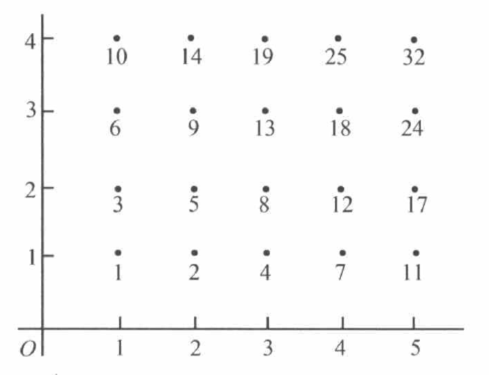
\includegraphics[width=6cm]{attachment/iShot_2023-08-04_15.19.06.png}
	\end{center}
	
	\underline{\textbf{证法二}}~~等价于证明$\mathbb{N}^n$是可数的.构造双射$\sigma : \mathbb{N}^n \to N, ~(\alpha _1,  \cdots , \alpha _n) \mapsto p_1^{\alpha _1} \cdots p_n^{\alpha _n}$.于是$\card \mathbb{N}^n = \card N = \card \mathbb{N}$.
\end{proof}

容易确定: 

\begin{proposition}
	$\card \mathbb{Z} = \card \mathbb{N} = \card \mathbb{Q} = \card \{ x: \exists n \in \mathbb{Z}_+, a_0,  \cdots , a_n \in \mathbb{Z}(a_0+a_1x+\cdots +a_nx^n=0) \}$.
\end{proposition}
\begin{remark}
	最后一个集合意思就是全体代数数构成的集合.
\end{remark}
\begin{proof}
	只证明最后一项.将$n$次整系数多项式的系数提取出来, 做双射于$\Z ^{n+1}$, 可以证明$n$次整系数多项式构成的集合是可数集. 进而所有整系数多项式构成的集合也是可数集. 
	
	利用代数基本定理可以完成后续证明. 
\end{proof}

虽然整数集、有理数集甚至代数数集都是可数的, 我们仍然能找到许多不可数集.

\begin{proposition}{}
	区间$(0, 1)$是不可数的.
\end{proposition}
\begin{proof}
	\underline{\textbf{证法一}}~~(Cantor对角线法) 设$(0, 1)$可数, 记$(0, 1)-\{ x/9: x \in \mathbb{Z},  1 \leq x \leq 8 \}=\{ a_1,  a_2,  \cdots , a_n , \cdots \}$, 并令$a_i$的十进制小数表示为$a_i=0.k_{i1}k_{i2}\cdots$.构作如下无限矩阵: 
	
	$$\begin{pmatrix}
 \color{red} k_{11} & k_{12} & k_{13} & \cdots & k_{1m} & \cdots \\
 k_{21} & \color{red} k_{22} & k_{23} & \cdots & k_{2m} & \cdots \\
 k_{31} & k_{32} & \color{red} k_{33} & \cdots & k_{3m} & \cdots \\
 \vdots & \vdots & \vdots & \color{red} \ddots & \vdots & \cdots \\
 k_{m1} & k_{m2} & k_{m3} & \cdots & \color{red} k_{mm} & \cdots \\
 \vdots & \vdots & \vdots & \vdots & \vdots & \color{red} \ddots
\end{pmatrix}.$$

	选取对角线上的数码$k_{11}, k_{22}, \cdots $.现在任取$k_j \neq k_{jj}$使得$1 \leq k_j \leq 8$.(假设不存在满足不等的$k_j$, 则$a_j$小数点后数码均相同, 必然为$\{ x/9: x \in \mathbb{Z},  1 \leq x \leq 8 \}$中某个元素, 矛盾).
	
	构造$a=0.k_1k_2k_3\cdots$, 由上面的构造可知$a$的十进制小数表示唯一, 又因为存在$m$使得$a=a_m$, 可得$k_m=k_{mm}$, 矛盾.
	
	\underline{\textbf{证法二}}~~之后我们会证明, 可数集一定是零测集(通俗地讲, 就是长度为$0$), 于是$\R$是不可数集. 
\end{proof}



\begin{corollary}{}
	实数集$\R$是不可数的.
\end{corollary}
\begin{remark}
	也可用闭区间套方法证明, 参阅后文. 
\end{remark}
\begin{proof}
	构造函数$f(x)=\tan \ssb{\pi x-\frac{\pi}{2}}$, 易知$f$为$(0, 1)$到$\R$的双射, 故$\card \R = \card (0, 1) > \card \mathbb{N}$.
\end{proof}

现在来看一些常用定理: 

\begin{lemma}{}
	任一无限集均存在可数子集.
\end{lemma}
\begin{proof}
	设无限集$X$, 取其中任意元素$x_0$放入集合$E$.接着在$X-\{ x_0 \}$中取任意元素$x_1$放入$E$.如此重复便得到一可数集$E \subseteq X$.
\end{proof}

\begin{theorem}{}
	无限集与至多可数集的并集与原无限集等势.
\end{theorem}
\begin{proof}
	有限集的情况显然; 考虑无限集$X$与可数集$Y=\{ y_1, y_2, \cdots \}$且$X \cap Y = \varnothing$.由上个引理可知$X$中存在一个可数集$E=\{ x_1, x_2, \cdots \}$.构造映射$f$使得$f(x_j)=x_{2j}, f(y_j)=x_{2j-1},  \forall j \in \mathbb{N}^*$和$f(x)=x, \forall x \in X-E$.容易验证$f$是$X \cup Y \to X$的双射.
\end{proof}

\begin{theorem}{}
	一个集合是无限集等且仅当其包含与自身等势的真子集.(这也被称作Dedekind无限)
\end{theorem}
\begin{proof}
	充分性: 设$X$存在真子集$E$与$X$等势, 假设$X$是有限集, 显然其不可能包含比自己基数大的集合, 矛盾.
	
	必要性: 任取$x \in X$, 可知$E: =X-\{x\}$满足$E \subset X$且$E$与$X$等势.
\end{proof}

从而我们可以证明: 

\begin{proposition}{}
	无理数集与实数集等势. 类似地有超越数(即不是代数数的实数)与实数集等势.
\end{proposition}

\begin{definition}{连续统}
	和实数集$\R$等势的集合称作\textit{连续统}(continuum). 连续统的基数称作\textit{连续基数}, 记作$\aleph _1$.
\end{definition}

一个著名的猜想: 连续统假设. 现在知道, 这个猜想不可能被ZFC公理系统证明或证伪.






\chapter{数列与函数的极限}

\section{数列的极限}

\subsection{数列极限的定义和性质}

\begin{definition}{序列}
	定义域为$\mathbb{N}$的映射称作\textit{序列}(sequence). 特别地, 值域为实数集的称作\textit{数列}(numerical sequence), 一般记作$\{ x_n \}$. 
\end{definition}

\begin{definition}{数列的极限}
	称数$A$为数列$\{ x_n \}$的\textit{极限}(limit), 如果对任意的$A$的邻域$N(A)$都存在$N$使得当$n \geq N$时$x_n \in N(A)$. 记为$$A = \lim_{n \to \infty} x_n ~~ \text{或} ~~ x_n \to A,~n \to \infty$$且称$\{ x_n \}$\textit{收敛}(convergent)于$A$. 若$\{ x_n \}$不存在极限, 则称其\textit{发散}(divergent). 
\end{definition}
\begin{remark}
	这里用邻域的写法只是方便理解“不断收缩至一个点”的过程. 等价的(且更为广泛的)写法是: $$\ssb{\lim_{n \to \infty} x_n = A} := \forall \varepsilon > 0 , \exists N \in \mathbb{N} (\forall n>N,|x_n-A|<\varepsilon ).$$
	这一定义也被称作“$\varepsilon -N$”定义.
\end{remark}

\begin{example}
	考虑如下数列在$n\to \infty$时是否存在极限并证明: $$x_n=\frac{1}{n},\qquad 1+\frac{(-1)^n}{n},\qquad \frac{1}{q^n}~(|q|>1),\qquad n^{(-1)^n}.$$
\end{example}
\begin{solution}
	前三个数列的极限存在,分别为$0,1,0$.最后一个数列极限不存在.
	
	(1)(2)对任意的$\varepsilon$,当$n>\lfloor \frac{1}{\varepsilon} \rfloor$时有$|\frac{1}{n} -0|<\varepsilon$和$|(1+\frac{(-1)^n}{n})-1|<\varepsilon$.
	
	(3)由引理\ref{lem:jxqlajimide}可知,对任意的$\varepsilon$都存在$N$使得$\frac{1}{|q|^N}<\varepsilon$,故当$n>N$时总有$|\frac{1}{a^n}-0|<\varepsilon$.
	
	(4)假设该数列存在极限$A$.当$A \neq 0$时,取$\varepsilon = \frac{|A|}{2}$可知当$n=2k+1 > \frac{2}{|A|}$时总有$|x_n-A|>\varepsilon$.当$a=0$时,取$\varepsilon =1$立得矛盾.
\end{solution}

数列的极限应当是良定义的.

\begin{proposition}{}
	收敛数列有且仅有一个极限.
\end{proposition}
\begin{proof}
	假设$\{ x_n \}$存在两个不同极限$A_1,A_2$, 取$\delta < \frac{1}{2}|A_1-A_2|$, 则存在$N_1,N_2$使得$x_n \in N_{\delta}(A_1),n > N_1$和$x_n \in N_{\delta}(A_2),n > N_2$. 然而当$n>\max \{ N_1,N_2 \}$时, $x_n \in N_{\delta}(A_1) \cap N_{\delta}(A_2) = \varnothing$, 矛盾. 
\end{proof}

将数列视作集合而定义数列的上(下)界、上(下)确界, 容易想到:

\begin{proposition}{}
	收敛数列必有界. 
\end{proposition}
\begin{proof}
	设$\{ x_n \}$极限为$A$. 令$\varepsilon = 1$可得当$n>N$时有$|x_n-A|<1$, 又因为$|x_n-A|>||x_n|-|A||$, 故$|x_n|<|A|-1$. 设$M=\max \{ x_1, \cdots ,x_N,|A|-1 \}$, 容易验证$M$为$\{ x_n \}$上界. 
\end{proof}

之前都是先猜测极限再给出证明, 利用数列极限的运算我们可以较为主动地算出极限. 

\begin{theorem}{数列极限的运算}
	设数列$\{ a_n \},\{ b_n \}$. 若$\lim_{n \to \infty} a_n=a,~\lim_{n \to \infty} b_n=b$, 则 \\
	(1)加减法$$\lim_{n \to \infty}{(a_n \pm b_n)} = a \pm b.$$
	(2)乘法$$\lim_{n \to \infty}{a_nb_n} = ab.$$
	(3)除法(当$b \neq 0$且$b_n \neq 0$时)$$\lim_{n \to \infty}{\frac{a_n}{b_n}} = \frac{a}{b}.$$
\end{theorem}
\begin{remark}
	利用上方性质容易推导:标量乘法(其中$c$为给定的实数)$$\lim_{n \to \infty}{ca_n}=ca.$$
	
\end{remark}
\begin{proof}
	(1)只需证明加法.任取$\varepsilon$,设存在$N_1,N_2$使得$|a_n-a|<\varepsilon /2,n>N_1$和$|b_n-b|<\varepsilon /2,n>N_2$,则当$n>\max \{ N_1,N_2 \}$时有$|a_n+b_n-(a+b)| \leq |a_n-a|+|b_n-b| < \varepsilon$.
	
	(2)先对$|a_nb_n-ab|$做一些放缩:$$|a_nb_n-ab| = |(a_n-a)b_n + a(b_n-b)| < |b_n||a_n-a| + |a||b_n-b|.$$
	设定$\{ b_n \}$的上界$M$,则进一步有$|a_nb_n-ab|<M|a_n-a| + |a||b_n-b|$.对任意$\varepsilon$,同上可知当$n$足够大时$|a_nb_n-ab|<\varepsilon$.
	
	(3)只需证明$\lim_{n\to \infty}(\frac{1}{b_n})=\frac{1}{b}$.考虑当$\lambda > |b_n-b| > ||b_n|-|b||$即$|b_n|>b-\lambda$且$b>\lambda$时有$$\left| \frac{1}{b_n} - \frac{1}{b} \right| = \frac{|b-b_n|}{|b||b_n|} < \frac{1}{|b(b-\lambda)|} \cdot |b-b_n|.$$
	同上可以证得对任意的$\varepsilon$都有$|\frac{1}{b_n}-\frac{1}{b} |<\varepsilon$.
\end{proof}

\subsection{数列极限的性质}

\begin{theorem}{夹逼定理}
	设三数列$\{ x_n \},\{ y_n \},\{ z_n \}$满足$x_n \leq y_n \leq z_n$对足够大的$n$总成立. 若$\{ x_n \}$与$\{ z_n \}$具有相同的极限, 则$\{ y_n \}$也具有相同的极限.
\end{theorem}
\begin{proof}
	记该极限值为$A$. 当$n$足够大时有$|x_n-A|<\varepsilon$和$|z_n-A|<\varepsilon$, 从而$A-\varepsilon < x_n \leq y_n \leq z_n < A+\varepsilon$, 即$|y_n-A|<\varepsilon$对足够大的$n$成立.
\end{proof}

\begin{theorem}{数列极限的保序性}
	对于两收敛数列$\{ x_n \},\{ y_n \}$,若$\lim_{n \to \infty} x_n < \lim_{n \to \infty} y_n$,则对足够大的$n$有$x_n<y_n$.
\end{theorem}
\begin{remark}
	取逆否命题立得,若$n$足够大时有$x_n \geq y_n$,则$\lim_{n \to \infty} x_n \geq \lim_{n \to \infty} y_n$.
\end{remark}
\begin{proof}
	选取两极限值$A,B$中间的某数$C$,当$n$足够大时有$|x_n-A|<C-A$和$|y_n-B|<B_C$,从而$x_n<C<y_n$对足够大的$n$成立.
\end{proof}

利用数列极限的运算和夹逼定理,我们可以处理很多数列极限(虽然有一些技术性较强).下面介绍一种求解未定式极限的方法,可以理解为离散版本的l'Hopital法则. 稍后会在习题里证明定理的情况一. 

\begin{theorem}{Stolz–Cesàro定理}
	设数列$\{ x_n \},\{ y_n \}$.那么$$\lim_{n\to \infty} \frac{x_n}{y_n} = \lim_{n\to \infty} \frac{x_{n+1}-x_n}{y_{n+1}-y_n}$$(假若极限存在)成立,如果满足以下两情况之一:
	\begin{itemize}
		\item ($\cdot / \infty$型)$\{ y_n \}$严格递增且发散(即认为极限为$+\infty$).
		\item ($0/0$型)$x_n,y_n \to 0$且$\{ y_n \}$严格单调.
	\end{itemize}
\end{theorem}

\newpage
\section{数列的敛散性}

\subsection{单调数列}

\begin{theorem}{单调有界定理}
	单调不减数列$\{ x_n \}$收敛于$\sup \{ x_n \}$当且仅当其有上界.
\end{theorem}
\begin{proof}
	只证明充分性:若$\{ x_n \}$存在上界,则其存在上确界$\sup \{ x_n \}$,意即对任意的$\varepsilon$都存在$N$使得$\sup \{x_n\}-\varepsilon < x_N \leq \sup \{ x_n \}$.取$n>N$可知$$\sup \{x_n\}-\varepsilon < x_N \leq a_n \leq \sup \{ x_n \}.$$
	这表明$\{ x_n \}$收敛于$\sup \{ x_n \}$.
\end{proof}

\begin{example}
	计算$\lim_{n\to \infty} \frac{n}{q^n}$,其中$q>1$.从而得到$\lim_{n\to \infty} \sqrt[n]{n}$.
\end{example}
\begin{solution}
	(1)定义$x_n=\frac{n}{q^n}$,则$x_{n+1}=\frac{n+1}{qn}x_n$.计算可得$$\lim_{n \to \infty} \frac{n+1}{qn} = \lim_{n \to \infty} \ssb{1+\frac{1}{n}} \cdot \lim_{n \to \infty} \frac{1}{q} = \frac{1}{q} < 1.$$
	于是当$n$足够大时$\{ x_n \}$单调递减,又显然$\{ x_n \}$有下界$0$,故其极限存在.由$$\lim_{n \to \infty} x_{n} = \lim_{n \to \infty} x_{n+1} = \lim_{n \to \infty} \frac{n+1}{qn} x_n = \frac{1}{q} \cdot \lim_{n \to \infty} x_n,$$可知该极限为$0$.
	
	(2)对给定的$\varepsilon > 0$,当$n$足够大时有$n<(1+\varepsilon)^n$,从而$\lim_{n\to \infty} \sqrt[n]{n} =1$.
\end{solution}

\begin{example}
	证明下列极限存在:$$\lim_{n\to \infty} \ssb{1+\frac{1}{n}}^n.$$
\end{example}
\begin{proof}
	\underline{\textbf{证法一}}~~定义$x_n=(1+\frac{1}{n})^n$. 由均值不等式有$$x_n = 1 \cdot \ssb{1+\frac{1}{n}} \cdots \ssb{1+\frac{1}{n}} < \ssb{\frac{1+n(1+\frac{1}{n})}{n+1}}^{n+1} = x_{n+1}. $$
	另一方面,由二项式定理, $$x_n = \sum_{i=0}^{n} \frac{1}{i!} \ssb{1-\frac{1}{n}} \cdots \ssb{1-\frac{i-1}{n}} < \sum_{i=0}^{n} \frac{1}{i!} < 1+1+\frac{1}{2}+\cdots + \frac{1}{2^{n-1}} = 3-\frac{1}{2^{n-1}}<3. $$
	由单调有界定理可知$\{ x_n \}$收敛. 
	
	\underline{\textbf{证法二}}~~定义$y_n=(1+\frac{1}{n})^{n+1}$, 由Bernoulli不等式可得$$\frac{y_n}{y_{n+1}} = \ssb{1+\frac{1}{n}}^n / \ssb{1+\frac{1}{n+1}}^{n+1} = \ssb{1+\frac{1}{(n+1)^2-1}}^{n+1} \cdot \frac{n+1}{n+2} > \ssb{1+\frac{n+1}{(n+1)^2-1}} \cdot \frac{n+1}{n+2} > 1. $$
	另外, $y_n>0$, 故$\{ y_n \}$极限存在. 
	
	亦容易验证$\{ x_n \}$与$\{ y_n \}$具有相同的极限.
\end{proof}

实际上,我们定义自然常数$e$为上述极限.在上个例子的证明中我们可以得到$$\ssb{1+\frac{1}{n}}^n < e < \ssb{1+\frac{1}{n}}^{n+1} ~~\Rightarrow ~~ \frac{1}{n+1} < \ln \frac{n+1}{n} < \frac{1}{n}.$$

\begin{example}
	证明下列极限存在:$$\lim_{n\to \infty} \ssb{ 1+\frac{1}{2}+\cdots + \frac{1}{n}-\ln n }.$$
\end{example}
\begin{proof}
	记$x_n=1+\frac{1}{2}+\cdots + \frac{1}{n}-\ln n$.计算可得$\{ x_n \}$单调递增且存在上界$1$.这里会用到上方的不等式.
\end{proof}

注意,调和级数发散,而调和级数(的部分和)与对数函数的差值收敛. 将该极限记作Euler常数$\gamma$.

\begin{theorem}{闭区间套定理} \label{thm:biqujmtc}
	设闭区间$I_n=[a_n,b_n]$,若$I_1 \supseteq I_2 \supseteq \cdots $,且$\lim_{n\to \infty} |a_n-b_n|=0$,则存在唯一的属于所有闭区间$c$. 
\end{theorem}
\begin{proof}
	显然$\{ a_n \},\{ b_n \}$均单调且有界,故存在极限.注意到$\lim_{n\to \infty} a_n = \lim_{n\to \infty} b_n$,记为$c$,即$\sup \{ a_n \} = \inf \{ b_n \} = c$,从而对任意$n$都有$a_n \leq c \leq b_n$,存在性即得证.
	
	现假设存在不同的$c'$亦满足$a_n \leq c' \leq b_n$对所有$n$都成立,那么$c' \leq \lim_{n\to \infty} b_n = \lim_{n\to \infty} a_n \leq c$,同理$c \leq c'$,即得$c=c'$,矛盾.
\end{proof}

\subsection{聚点与上下极限}

\begin{definition}{子列}
	设数列$\{ x_n \}$.若单调递增数列$\{ n_k \} \subseteq \mathbb{Z}$,则称$\{ x_n:n \in  \{ n_k \} \}$是$\{ x_n \}$的一个\textit{子列}(subsequence).
\end{definition}

\begin{proposition}{}
	设数列$\{ x_n \}$可以划分为一些子列$\{ x_{1_n} \},\{ x_{2_n} \},\cdots ,\{ x_{k_n} \}$. 则$x_n \to A$当且仅当对所有$j$, $x_{j_n} \to A$. 
\end{proposition}
\begin{proof}
	必要性: 任取$\varepsilon >0$, 对$n>N$有$|x_n-A|<\varepsilon$, 那么对任意一个子列, 归纳易得$j_n>n>N$, 此时总有$|x_{j_n}-A|<\varepsilon$.
	
	充分性: 对任意的$\varepsilon >0$, 设存在$N_1,\cdots ,N_k$满足当$n>N_j$时有$|x_{j_n}-A|<\varepsilon$, 则取$N=\max \{ N_1,\cdots ,N_k \}$可知当$n>N$时有$|x_n-A|<\varepsilon$.
\end{proof}

\begin{definition}{聚点}
	称$p$是集合$X$的\textit{聚点}(limit point), 如果任意$p$的邻域都包含$X$的一个无穷子集.
\end{definition}
\begin{remark}
	等价的说法是: 任意$p$的空心邻域与$X$的交集非空. 
\end{remark}

下面的看法非常有用:

\begin{proposition}{}
	数列的聚点就是某个子列的极限.
\end{proposition}
\begin{proof}
	一方面,设数列$\{ x_n \}$具有聚点$p$.对任意$k$,我们选取$|x_{n_k}-p|<\frac{1}{k}$,则由$p$为聚点可知存在$n_{k+1}>n_k$满足$|x_{n_{k+1}}-p|<\frac{1}{k+1}$.由于$\frac{1}{k} \to 0$,故对任意$\varepsilon >0$都存在足够大的$k$满足$|x_{n_k}-p||<\frac{1}{k}<\varepsilon$,即子列$\{ x_{n_k} \}$收敛于$p$.
	
	另一方面,设数列$\{ x_n \}$的某个子列$\{ x_{k_n} \}$收敛于$p$.对任意$N_{\delta}(p)$都存在$N$使得当$k_n>N$时有$x_{k_n} \in N_{\delta}(p)$,又$\{ x_{k_n} \}$是一个无穷数列,故$N_{\delta}(p)$包含$\{ x_n \}$的一个无穷子集.
\end{proof}

\begin{lemma}{Bolzano-Weierstrass引理}
	有界无限实数集$X$必有聚点.
\end{lemma}
\begin{proof}
	由$X$有界可知存在闭区间$I \supseteq X$.我们声明$I$中至少有一个元素是$X$的聚点,否则对任意$x \in I$都存在邻域$N(x)$不包含$X$中无限个元素.然而由于$\{ N(x):x \in I \}$构成$X$的开覆盖,由Henite-Borel定理可知存在一些邻域$\{ U(x_1),\cdots ,U(x_n) \}$亦能覆盖$X$,这时可以得到$X$中只包含有限个元素,与$X$是无限集矛盾.
\end{proof}

\begin{theorem}{Bolzano-Weierstrass定理}
	有界无限实数列必有收敛子列.
\end{theorem}
\begin{proof}
	\underline{\textbf{证法一}}~~如果数列$\{ x_n \}$的值域有限, 则存在无穷个$x' \in x_n$相等, 那么子列$\{ x' \}$为常数列, 从而收敛. 现在设$\{ x_n \}$值域无限, 由引理可知$\{ x_n \}$存在聚点, 所以存在某个子列, 其极限恰为该聚点.
	
	\underline{\textbf{证法二}}~~若$\{ x_n \}$单调,由单调收敛定理知其存在极限.若$\{ x_n \}$不单调,考虑这样的$N$:对所有的$n>N$都有$x_n<x_N$.若这样的$N$有无穷多个,取所有的$\{ x_N \}$即得单调递减;若这样的$N$只有有限个,则最后一个$x_N$之后存在单调递增的子列.
\end{proof}

如果认为$+\infty ,-\infty$也是实数的话(即所谓扩展实数集), 容易得到下方的命题:

\begin{proposition}{}
	实数数列包含收敛于实数或$\pm \infty$的子列.
\end{proposition}

\begin{definition}{上极限,下极限}
	设数列$\{ x_n \}$,定义$\liminf_{k\to \infty} x_k:=\lim_{n\to \infty} \inf_{k \geq n} x_k$为$\{ x_n \}$的\textit{下极限}(inferior limit).类似定义$\limsup_{k\to \infty} x_k$为$\{ x_n \}$的\textit{上极限}(superior limit).上极限和下极限可以为$\pm \infty$.
\end{definition}

记$i_n=\inf_{k\geq n}x_k$, $i=\lim_{n\to \infty} i_{n}$, 容易验证$\{ i_n \}$是单调不减的. 于是$$i=\lim_{n\to \infty} i_{n} \quad \Leftrightarrow \quad \forall \varepsilon >0, \exists N>0 (\forall n>N, i-i_n<\varepsilon) \quad \Leftrightarrow \quad \forall \varepsilon >0, \exists N>0 (\forall n>N, i-\varepsilon<x_n).$$
上极限也有类似的描述方法. 

在以下的论述中,我们认为\textit{部分极限}(partial limit)是聚点或者$\pm \infty$.

\begin{proposition}{}
	数列上下极限分别是其部分极限的最大、小元素.
\end{proposition}
\begin{proof}
	先来证明:有界数列的上下极限分别是其部分极限的最大、小元素.以下极限为例:
	
	定义$i_n=\inf_{k\geq n}x_k$,记$i=\lim_{n\to \infty} i_{n}$,自然有$i_n$单调不减趋于$i$.我们可以归纳地得到所有$k_n$满足$k_n<k_{n+1}$且$i_{k_n} \leq x_{k_n} < i_{k_n}+\frac{1}{n}$.由于$\lim_{n\to \infty} i_{k_n} = \lim_{n\to \infty} (i_{k_n}+\frac{1}{n} ) = i$,由夹逼定理得$\lim_{n\to \infty} x_{k_n}=i$,即下极限是某个部分极限.声明该部分极限为最小的:对于任意$\varepsilon >0$,足够大的$n$满足$i-\varepsilon < i_n \leq x_k$对所有$k \geq n$成立.由$\varepsilon$的任意性可知所有的部分极限至少为$i$.
	
	接着证明无界的情况.例如若无下界,即存在一个极限为$-\infty$的子列,容易得到$i=-\infty$,我们约定其为部分极限的最小元素.
\end{proof}

容易验证, 数列收敛当且仅当其只存在一个聚点. 由上方的命题马上得到: 数列收敛当且仅当其上下极限相等. 

\subsection{Cauchy收敛准则}

\begin{definition}{Cauchy列}
	一个数列$\{ x_n \}$被称作\textit{Cauchy列}(Cauchy sequence),如果对于任意的$\varepsilon >0$都存在自然数$N$使得$|x_m-x_n|<\varepsilon$对$m,n>N$恒成立.
\end{definition}

\begin{theorem}{Cauchy收敛准则}
	一个数列收敛当且仅当它是一个Cauchy列.
\end{theorem}
\begin{remark}
	将Cauchy收敛准则和单调收敛原理对比可以发现:前者是收敛的充要条件,而后者只是充分条件.
\end{remark}
\begin{proof}
	必要性:设数列$\{ x_n \}$收敛于$A$. 则对任意$\varepsilon >0$都存在足够大的$m$满足$|x_m-A|<\varepsilon ,|x_n-A|<\varepsilon$, 从而可得$|x_m-x_n|<|x_m-A|+|x_n-A|<2\varepsilon$对足够大的$m,n$成立. 
	
	充分性:容易证明Cauchy列$\{ x_n \}$有界. 由Bolzano-Weierstrass定理可知$\{ x_n \}$存在某个子列$\{ x_{n_k} \}$有极限$A$. 对任意$\varepsilon >0$, 当$n_k$足够大时有$|x_{n_k} - A|<\varepsilon$. 从而当$n$足够大时有$|x_n-A|<|x_n-x_{n_k}|+|x_{n_k}-A|<2\varepsilon$. 
\end{proof}

\subsection{实数完备性定理: 总结}

至此,我们按照$$\textit{确界原理} \Rightarrow \textit{单调收敛定理} \Rightarrow \textit{闭区间套定理} \Rightarrow \textit{Bolzano-Weierstrass定理} \Rightarrow \textit{Cauchy收敛准则}$$的路线证明了实数完备性定理中所有定理的正确性.是时候补上等价性的最后一块砖了:

\begin{proposition}{}
	Cauchy收敛准则可以推导确界原理.从而,实数完备性的7个定理互相等价.
\end{proposition}
\begin{remark}
	实际上还要加上Archimedes性质才能等价. 
\end{remark}
\begin{proof}
	设非空集合$X$存在上界,由Archimedes性质可知,对任意的$n$都存在唯一的整数$k_n$使得$q_n=\frac{k_n}{n}$是$X$的上界而$\frac{k_n-1}{n}$不是.我们断言$\{ q_n \}$是一个Cauchy列,从而其存在极限$q$.这里的$q$显然是$X$的上界,而对每个$n$都存在$x \in X$使得$x>q_n-\frac{1}{n}$,容易得到$q$就是$X$的上确界.
	
	断言的证明:对任意的$m,n$分别存在$x_m,x_n \in X$使得$q_m-\frac{1}{m} < x_m,q_n-\frac{1}{n} < x_n$,而$q_m \geq x_n,q_n \geq x_m$,所以$|q_m-q_n|<\max \{ \frac{1}{m},\frac{1}{n} \}$,易知断言成立.
\end{proof}

\newpage
\section*{补充习题} \label{sec:ex3.1}

\subsection*{A: Toeplitz变换与Stolz定理}

开胃菜: 设$\{ a_n \}$是实数序列, 定义算术平均值序列$\sigma _n = \frac{a_1+\cdots + a_n}{n}, n \in \mathbb{N}^{*}$. 
\vspace{1em}

\circled{A1}~~设$\lim_{n\to \infty} a_n=a$, 则$\lim_{n\to \infty} \sigma _n=a$. 
\vspace{1em}

定义无限非负下三角矩阵$T=(t_{nk})$为一个Toeplitz矩阵, 若其满足

1) 对任意$n \in \mathbb{N}^{*}$都有$\sum_{k=1}^{n} t_{nk}=1$; \qquad 2) 对任意$k \in \mathbb{N}^{*}$都有$\lim_{n\to \infty} t_{nk}=0$.

对于数列$\{ a_n \}$, 称$b_n=\sum_{k=1}^{n} t_{nk}a_k$构成的序列$\{ b_n \}$为其关于$T$的Toeplitz变换. (不严谨地, 即将$\{ a_n \},\{ b_n \}$竖写作向量$\alpha ,\beta$, 有$T\alpha = \beta$)

作为例子(提示), 我们注意到A1中$\{ \sigma _n \}$就是$\{ a_n \}$关于$$\begin{pmatrix}
 1 &  &  &  & \\
 \frac{1}{2}  & \frac{1}{2} &  &  & \\
 \vdots & \vdots & \ddots &  & \\
 \frac{1}{n}  & \frac{1}{n} & \cdots & \frac{1}{n} & \\
 \vdots & \vdots & \vdots & \vdots & \ddots
\end{pmatrix}$$的Toeplitz变换. 
\vspace{1em}

\circled{A2}~~(Silverman-Toeplitz) 若$\lim_{n\to \infty} a_n=a$, 则$\lim_{n\to \infty} b_n=a$. 
\vspace{1em}

\circled{A3}~~(Stolz-Cesáro) 设数列$\{ a_n \}$和$\{ b_n \}$, 其中$\{ b_n \}$严格递增, 且$\lim_{n\to \infty} b_n = \infty$. 那么$$\lim_{n\to \infty} \frac{a_n}{b_n} = \lim_{n\to \infty} \frac{a_n-a_{n-1}}{b_n-b_{n-1}}. $$
(前提是右侧极限存在且为实数)
\vspace{1em}

\subsection*{B: 数列的上下极限}

\circled{B1}~~证明, 数列$\{ x_n \}$上下极限的三种定义方式是等价的: (以下极限为例)

a) $\liminf_{k\to \infty} x_k:=\lim_{n\to \infty} \inf_{k \geq n} x_k$;\qquad b) $\liminf_{k\to \infty} x_k:= \min  \{\{ x_n \}\text{的聚点} \}$; 

c) $\liminf_{k\to \infty} x_k:= \sup \{ a\in \R \cup \{ -\infty \}: \forall \varepsilon >0, \exists N \in \mathbb{N}^{*} (\forall n>N, x_n>a-\varepsilon ) \}$
\vspace{1em}

\circled{B2}~~设数列$\{ a_n \}, \{ b_n \}$, 则其下极限是超可加的, 上极限是次可加的, 即
\begin{align*}
	\underline{\liminf_{n\to \infty} a_n + \liminf_{n\to \infty} b_n \leq \liminf_{n\to \infty} (a_n+b_n) }&\leq \liminf_{n\to \infty} a_n + \limsup_{n\to \infty} b_n \\
	&\leq \underline{\limsup_{n\to \infty} (a_n+b_n) \leq \limsup_{n\to \infty} a_n + \limsup_{n\to \infty} b_n}.
\end{align*}

特别地, $$\liminf_{n\to \infty} (a_n+b_n)  = \lim_{n\to \infty} a_n + \liminf_{n\to \infty} b_n , \qquad \limsup_{n\to \infty} (a_n+b_n)  = \lim_{n\to \infty} a_n + \limsup_{n\to \infty} b_n. $$

\circled{B3}-1~~设非负数列$\{ a_n \}, \{ b_n \}$, 类似于B2有如下结论: 
\begin{align*}
	\underline{\ssb{\liminf_{n\to \infty} a_n}\ssb{ \liminf_{n\to \infty} b_n} \leq \liminf_{n\to \infty} (a_nb_n) } &\leq \ssb{\liminf_{n\to \infty} a_n}\ssb{ \limsup_{n\to \infty} b_n} \\
	&\leq \underline{\limsup_{n\to \infty} (a_nb_n) \leq \ssb{\limsup_{n\to \infty} a_n}\ssb{ \limsup_{n\to \infty} b_n}}.
\end{align*}

\circled{B3}-2~~特别地, 对非负数列$\{ a_n \}$和任意数列$\{ b_n \}$都有$$\liminf_{n\to \infty} (a_nb_n) = \ssb{\lim_{n\to \infty} a_n} \ssb{\liminf_{n\to \infty} b_n}, \qquad \limsup_{n\to \infty} (a_nb_n) = \ssb{\lim_{n\to \infty} a_n} \ssb{\limsup_{n\to \infty} b_n}.$$

\circled{B4}~~设正数列$\{ a_n \}$, 则$$\liminf_{n\to \infty} \frac{a_{n+1}}{a_n} \leq \liminf_{n\to \infty} \sqrt[n]{a_n} \leq \limsup_{n\to \infty} \sqrt[n]{a_n} \leq \limsup_{n\to \infty} \frac{a_{n+1}}{a_n}. $$




\newpage
\section{数项级数}

\subsection{基本概念}

\begin{definition}{级数}
	\vspace{-2em}
	\begin{itemize}
		\item 设数列$\{ a_n \}$. 我们简记$a_1+a_2+\cdots +a_n + \cdots = \sum_{n=1}^{\infty} a_n$, 称之为\textit{级数}(series).
		\item 如果部分和数列$s_n=\sum_{k=1}^n a_n$的极限$s$存在, 则称该极限为级数的\textit{和}(sum), 记作$s=\sum_{n=1}^{\infty} a_n$,并称该级数\textit{收敛}(convergent), 否则\textit{发散}(divergent).
	\end{itemize}
\end{definition}

\begin{example}
	$(a)$~\textit{几何级数}$1+q+q^2+\cdots +q^n+\cdots$在$|q|<1$时收敛于$\frac{1-q^n}{1-q}$,而$|q|\geq 1$时发散.
	
	$(b)$~\textit{调和级数}$1+\frac{1}{2}+\frac{1}{3}+\cdots + \frac{1}{n} + \cdots$发散.
\end{example}

\begin{proposition}{}
	当级数中只有有限项改变时, 级数的敛散性不变.
\end{proposition}
\begin{remark}
	但级数的和有可能改变. 
\end{remark}
\begin{proof}
	对级数应用Cauchy收敛准则可得: 级数$\sum_{n=1}^{\infty} a_n$收敛当且仅当对任意的$\varepsilon >0$都存在足够大的$m \leq n$使得$|a_m + \cdots + a_n|<\varepsilon$. 从而上述命题显然.
\end{proof}

\begin{proposition}{}
	级数收敛的必要条件是其所有项构成的数列极限为$0$.
\end{proposition}
\begin{proof}
	设级数部分和$s_n \to s$,即对任意的$\varepsilon >0$都存在足够大的$n$使得$|s_n-s|<\varepsilon$,从而$a_n \to 0$.
\end{proof}

\begin{example}
	级数$1+(-1)+1+(-1)+\cdots +(-1)^{n+1}+\cdots$发散,然而将该级数中的一些项合并与交换位置,可以得到:
	$$(1-1)+(1-1)+\cdots ~~\textit{收敛于}~0, \qquad 1+(-1+1)+(-1+1)+\cdots ~~\textit{收敛于}~1,$$
	\begin{center}
		$1+1+(-1)+1+(-1)+\cdots \textit{收敛于}~2.$
	\end{center}
\end{example}

这个例子中意外出现的原因比较明显: 在对有限项进行交换、结合等操作时不会造成求和的改变, 然而无限操作可能会影响整个部分和序列. 

下面来看一个进行无穷次操作的例子:

\begin{example}
	已知调和级数的部分和可以按照如下方式估计:$s_n=\gamma + \ln n + o(1)$.对于交错调和级数$1-\frac{1}{2}+\frac{1}{3}-\frac{1}{4}+\cdots + \frac{(-1)^{n+1}}{n}+\cdots $,可以通过某些重排,使得新级数的和为任意实数.
\end{example}
\begin{proof}
	我们选取其中的偶数项,记$s_{n-}=-\sum_{k=1}^{n} \frac{1}{2n} = -\frac{1}{2}\gamma -\frac{1}{2}\ln n+o(1)$.那么奇数项的部分和$s_{n+}=s_n-s_{n-}=\ln 2+\frac{1}{2}\gamma + \frac{1}{2}\ln n + o(1)$.这两个部分和都是发散的.
	
	对任意实数$x$,声明以下算法:第$1$步,将所有奇数项依次放入新级数,直到这些数的和超过$x$;第$2$步,将所有偶数项依次放入新级数,直到所有的和低于$x$.
	
	其中,由于交错取出的部分和序列均发散,每一步必然都会超出$x$或低于$x$,意味着以上算法将会不断重复.注意到,在跨越$x$的瞬间,只能变化$\frac{1}{n}$,而$\frac{1}{n} \to 0$,所以最后的新级数和即为$x$.
\end{proof}

从这个例子里可以抽象出两个特点: 一个级数满足上述性质, 如果它的正项所成级数与负项所成级数均发散, 并且单独的每一项趋于$0$. 我们可以有如下定义: 

\begin{definition}{绝对收敛,条件收敛}
	\vspace{-2em}
	\begin{itemize}
		\item 称一个级数$\sum_{n=1}^{\infty} a_n$\textit{绝对收敛}(absolutely convergent), 如果$\sum_{n=1}^{\infty} a_n$和$\sum_{n=1}^{\infty} |a_n|$均收敛. 
		\item 反之,若$\sum_{n=1}^{\infty} a_n$收敛而$\sum_{n=1}^{\infty} |a_n|$发散,则称该级数\textit{条件收敛}(conditionally convergent). 
	\end{itemize}
\end{definition}
\begin{remark}
	可以将绝对收敛的条件简化为$\sum_{n=1}^{\infty} |a_n|$收敛.
\end{remark}

从而有:

\begin{theorem}{Riemann重排定理}
	对一个条件收敛的无穷级数, 可以给出一种重排方案, 使得新级数的和等于任意实数或$\pm \infty$. 
\end{theorem}

取逆否命题知, 无论如何重排级数和均不变的级数是绝对收敛的. 实际上, 这句话反过来亦成立. 

\begin{proposition}{}
	设级数$\sum_{n=1}^{\infty} a_n$绝对收敛, 则任意重排后的级数$\sum_{n=1}^{\infty} b_n$也收敛, 且$\sum_{n=1}^{\infty} a_n = \sum_{n=1}^{\infty} b_n$. 
\end{proposition}
\begin{proof}
	(1) 先证明, 若$\sum_{n=1}^{\infty} a_n$是非负项级数则命题成立. 实际上, 对任意$N$都存在$n>N$使得$$\sum_{k=1}^{N}b_k \leq \sum_{k=1}^{n}a_k \leq \sum_{k=1}^{\infty} a_k.$$
	于是$\sum_{n=1}^{\infty} b_n$收敛. 特别地, 令$N\to \infty$可知$\sum_{n=1}^{\infty} b_n \leq \sum_{n=1}^{\infty} a_n$. 同理可得$\sum_{n=1}^{\infty} a_n \leq \sum_{n=1}^{\infty} b_n$. 
	
	(2) 再证明原命题. 将$\sum_{n=1}^{\infty} a_n$拆成$\sum_{n=1}^{\infty} a_n^+ - \sum_{n=1}^{\infty} a_n^-$, 其中$a_n^+,a_n^- \geq 0$. 容易证明$\sum_{n=1}^{\infty} a_n^+$和$\sum_{n=1}^{\infty} a_n^-$都是收敛的. 同样地拆解$\sum_{n=1}^{\infty} b_n$. 
	
	由(1)可知$\sum_{n=1}^{\infty} a_n^+ = \sum_{n=1}^{\infty} b_n^+$, $\sum_{n=1}^{\infty} a_n^- = \sum_{n=1}^{\infty} b_n^-$, 那么$\sum_{n=1}^{\infty} b_n = \sum_{k=1}^{\infty} b_n^+ - \sum_{n=1}^{\infty} b_n^- = \sum_{k=1}^{\infty} a_n^+ - \sum_{n=1}^{\infty} a_n^- = \sum_{n=1}^{\infty} a_n$. 
\end{proof}

用同样的想法, 可以证明如下命题: 

\begin{proposition}{}
	设级数$\sum_{k=1}^{\infty} a_k$和$\sum_{k=1}^{\infty} b_k$绝对收敛, $\{ c_n \}$是$\{ a_ib_j \}$的一个重排, 则$\sum_{n=1}^{\infty} c_n$收敛且
	\begin{center}
		$\displaystyle \sum_{n=1}^{\infty} c_n = \left(\sum_{k=1}^{\infty} a_k \right)\left(\sum_{k=1}^{\infty} b_k \right).$
	\end{center}
\end{proposition}
\begin{proof}
	(1) 先证明, 若$\sum_{k=1}^{\infty} a_k$和$\sum_{k=1}^{\infty} b_k$均为非负项级数则命题成立. 
	
	容易证明$\sum_{n=1}^{\infty} c_n$的部分和有界, 从而收敛. 待定$\varepsilon _1,\varepsilon _2$, 则存在足够大的$n$使得$$|\sum_{k=1}^{n} a_k - \sum_{k=1}^{\infty} a_k| < \varepsilon _1, \quad |\sum_{k=1}^{n} b_k - \sum_{k=1}^{\infty} b_k| < \varepsilon _2.$$
	所以
	\begin{align*}
		& \big|(\sum_{k=1}^{n} a_k)(\sum_{k=1}^{n} b_k) -(\sum_{k=1}^{\infty} a_k)(\sum_{k=1}^{\infty} b_k)  \big| \\
		& \leq \big|(\sum_{k=1}^{n} a_k)(\sum_{k=1}^{n} b_k)-(\sum_{k=1}^{n} a_k)(\sum_{k=1}^{\infty} b_k)\big|+\big|(\sum_{k=1}^{n} a_k)(\sum_{k=1}^{\infty} b_k)-(\sum_{k=1}^{\infty} a_k)(\sum_{k=1}^{\infty} b_k)\big| \\
		& \leq \varepsilon _1 \big| \sum_{k=1}^{\infty} a_k \big| + \varepsilon _2 \big| \sum_{k=1}^{\infty} b_k \big|.
	\end{align*}
	通过恰当地选取$\varepsilon _1, \varepsilon _2$即可证明. 
	
	(2) 再证明原命题. 同上拆解$\sum_{k=1}^{\infty} a_k$和$\sum_{k=1}^{\infty} b_k$. 
	
	由于$c_n=a_ib_j=a_i^+b_j^+ + a_i^-b_j^- - (a_i^+b_j^- + a_i^-b_j^+)$, 实际上我们有
	\begin{align*}
		\sum_{n=1}^{\infty} c_n &= (\sum_{k=1}^{\infty} a_k^+)(\sum_{k=1}^{\infty} b_k^+) + (\sum_{k=1}^{\infty} a_k^-)(\sum_{k=1}^{\infty} b_k^-) - (\sum_{k=1}^{\infty} a_k^+)(\sum_{k=1}^{\infty} b_k^-) - (\sum_{k=1}^{\infty} a_k^-)(\sum_{k=1}^{\infty} b_k^+) \\
		&= (\sum_{k=1}^{\infty} a_k)(\sum_{k=1}^{\infty} b_k).
	\end{align*}
\end{proof}
\begin{remark}
	按照类似的思路, 可以进一步将命题推广到复数项级数. 
\end{remark}

\subsection{级数敛散性的判别法}

需要声明的是, 关于级数敛散性的判别方法非常多, 这里无法全部列举. 感兴趣的可以参考\href{https://en.wikipedia.org/wiki/Convergence_tests}{这个网页}\footnote{https://en.wikipedia.org/wiki/Convergence\_tests}. 

\begin{lemma}{}
	非负项级数收敛当且仅当部分和序列有上界.
\end{lemma}

\begin{proposition}{比较判别法}
	对于非负项级数$\sum_{n=1}^{\infty} a_n,\sum_{n=1}^{\infty} b_n$,若对足够大的$n$均有$a_n \leq b_n$,则$\sum_{n=1}^{\infty} b_n$收敛可推$\sum_{n=1}^{\infty} a_n$收敛.
\end{proposition}
\begin{proof}
	不妨设对所有的$n$都有$a_n \leq b_n$,则$A_n = \sum_{k=1}^{n} a_n \leq \sum_{k=1}^n b_n = B_n$.若$B_n \to B$,则$\{ B_n \}$存在上界$B$,从而$\{ A_n \}$亦有上界$B$,由引理可知$\sum_{n=1}^{\infty} a_n$收敛.
\end{proof}

\begin{example}
	由于$\frac{1}{n^2}<\frac{1}{n(n-1)}$,而$\sum_{n=1}^{\infty}\frac{1}{n(n-1)} = \lim_{n\to \infty} \sum_{k=1}^{n} \frac{1}{k(k+1)} = \lim_{n\to \infty} (1-\frac{1}{n+1})=1$,故$\sum_{n=1}^{\infty} \frac{1}{n^2}$收敛.(实际上它等于$\frac{\pi ^2}{6}$,不过暂时无法证明)
\end{example}

\begin{corollary}{比较判别法的极限形式}
	设非负项级数$\sum_{n=1}^{\infty} a_n,\sum_{n=1}^{\infty} b_n$, 记$\alpha=\lim_{n\to \infty} \frac{a_n}{b_n}$, 则有: 
	
	a) 当$0<\alpha <\infty$时, $\sum_{n=1}^{\infty} a_n$和$\sum_{n=1}^{\infty} b_n$敛散性相同. 
	
	b) 当$\alpha =0$时, 由$\sum_{n=1}^{\infty} b_n$收敛可推$\sum_{n=1}^{\infty} a_n$收敛. 
	
	c) 当$\alpha = \infty$时, 由$\sum_{n=1}^{\infty} b_n$发散可推$\sum_{n=1}^{\infty} a_n$发散. 
\end{corollary}
\begin{proof}
	a) 对充分大的$n$有$|\frac{a_n}{b_n}-\alpha |<\frac{\alpha}{2}$即$\frac{\alpha}{2} b_n<a_n<\frac{3\alpha}{2}a_n$, 故两级数敛散性相同. 
	
	b) 对充分大的$n$有$a_n<b_n$, 即得. 
	
	c) 对充分大的$n$有$a_n>b_n$, 即得. 
\end{proof}

\begin{example}
	求所有的$x \in \R$使得下述级数收敛: $$\sum_{n=1}^{\infty} \frac{n+\sin n}{\sqrt{n^3+\ln n +1}}. $$
\end{example}
\begin{solution}
	显然$\frac{n+\sin n}{\sqrt{n^3+\ln n +1}} / \frac{1}{\sqrt{n}} \to 1$, 由$\sum_{n=1}^{\infty} \frac{1}{\sqrt{n}}$发散可知原级数对任意$x \in \R$均发散. 
\end{solution}

\begin{corollary}{Weierstrass判别法}
	设级数$\sum_{n=1}^{\infty} a_n,\sum_{n=1}^{\infty} b_n$,若对足够大的$n$有$|a_n|<b_n$,则$\sum_{n=1}^{\infty} b_n$收敛可推$\sum_{n=1}^{\infty} a_n$绝对收敛.
\end{corollary}

\begin{proposition}{Cauchy判别法}
	设级数$\sum_{n=1}^{\infty} a_n$,记$\alpha = \limsup_{n\to \infty} \sqrt[n]{|a_n|}$.则有:
	
	a) 当$\alpha >1$时,级数$\sum_{n=1}^{\infty} a_n$发散;
	
	b) 当$\alpha <1$时,级数$\sum_{n=1}^{\infty} a_n$绝对收敛;
	
	c) 当$\alpha =1$时,级数$\sum_{n=1}^{\infty} a_n$可能发散或绝对收敛.
\end{proposition}
\begin{proof}
	a) 用反证法.假设级数收敛,则$a_n \to 0$.但由题知存在$\{ a_n \}$的子列$\{ a_{n_k} \}$使得$\lim_{k\to \infty} \sqrt[n_k]{|a_{n_k}|} = \alpha > 1$,由极限保序性知对足够大的$k$有$a_{n_k}>1$,矛盾.
	
	b) 构造级数$Q=\sum_{n=1}^{\infty} q^n$,其中$q$满足$\alpha < q <1$.熟知$Q$收敛,而对足够大的$n$有$\sqrt[n]{|a_n|}<q$即$|a_n|<q^n$,故原级数绝对收敛.
	
	c) 熟知$\sum_{n=1}^{\infty} \frac{1}{n}$和$\sum_{n=1}^{\infty} \frac{1}{n^2}$分别发散和绝对收敛,它们都满足c)的条件.
\end{proof}

\begin{example}
	求所有$x \in \R$使得下述级数收敛:$$\sum_{n=1}^{\infty} \ssb{2+(-1)^n}^n x^n.$$
\end{example}
\begin{solution}
	计算$\alpha = \limsup_{n\to \infty} \sqrt[n]{\ssb{2+(-1)^n}^n |x|^n}= |x|\limsup_{n\to \infty} (2+(-1)^n)=3|x|$.故当$|x|<\frac{1}{3}$时,原级数绝对收敛;当$|x|=\frac{1}{3}$时,注意到对所有的$n=2k$有$\ssb{2+(-1)^n}^n x^n = (3|x|)^{2k}=1$,原级数发散.
\end{solution}

\begin{proposition}{d’Alembert判别法}
	若对于级数$\sum_{n=1}^{\infty} a_n$, 极限$\lim_{n\to \infty}|\frac{a_{n+1}}{a_n} |=\alpha$存在, 则有:
	
	a) 当$\alpha >1$时,级数$\sum_{n=1}^{\infty} a_n$发散;
	
	b) 当$\alpha <1$时,级数$\sum_{n=1}^{\infty} a_n$绝对收敛;
	
	c) 当$\alpha =1$时,级数$\sum_{n=1}^{\infty} a_n$可能发散或绝对收敛.
\end{proposition}
\begin{proof}
	a) 对足够大的$n$有$|a_{n+1}|>|a_n|$,显然与$a_n\to 0$矛盾.
	
	b) 取$q$使得$\alpha < q <1$,则对足够大$n$有$|a_{n+1}|<q|a_n|<\cdots < q^n|a_1|$,构造级数$\sum_{n=0}^{\infty} |a_1|q^n$显然收敛,故原级数绝对收敛.
	
	c) 同上个命题中的例子.
\end{proof}

\begin{example}
	求所有的$x \in \R$使得下述级数收敛: 
	\begin{center}
		$\displaystyle \sum_{n=1}^{\infty} \frac{1}{n!}x^n.$
	\end{center}
\end{example}
\begin{solution}
	计算$\alpha = \lim_{n\to \infty}|\frac{a_{n+1}}{a_n} | = \lim_{n\to \infty} \frac{|x|}{n+1} = 0$,故原级数对所有实数$x$都是收敛的.
\end{solution}

类似于Cauchy判别法, d'Alembert也有上下极限的版本: 

\begin{corollary}{}
	设级数$\sum_{n=1}^{\infty} a_n$, 记$\limsup_{n\to \infty} |\frac{a_{n+1}}{a_n}|=L$, $\liminf_{n\to \infty} |\frac{a_{n+1}}{a_n}|=\ell$. 则有: 
	
	a) 当$1 < \ell < L$时, 级数$\sum_{n=1}^{\infty} a_n$发散. 
	
	b) 当$\ell < L < 1$时, 级数$\sum_{n=1}^{\infty} a_n$绝对收敛. 
	
	c) 当$\ell = 1$或$L =1$时, 级数$\sum_{n=1}^{\infty} a_n$可能发散或绝对收敛. 
\end{corollary}
\begin{proof}
	a) 构造$\alpha$使得$1<\alpha <\ell$, 则对足够大的$n$有$|\frac{a_{n+1}}{a_n}|>\alpha >1$, 于是原级数发散. 
	
	b) 构造$\alpha$使得$L<\alpha <1$, 则对足够大的$n$有$|\frac{a_{n+1}}{a_n}|<\alpha <1$, 于是原级数绝对收敛. 
\end{proof}

上一节的补充习题B4告诉我们, d'Alembert判别法的适用范围比Cauchy判别法更窄(但是一般更好用). 

\begin{proposition}{Cauchy}
	若非负数列$\{ a_n \}$单调不增,则级数$\sum_{n=1}^{\infty} a_n$收敛当且仅当级数$\sum_{k=0}^{\infty} 2^ka_{2^k}$收敛.
\end{proposition}
\begin{remark}
	这就是所谓“按$2^k$为长度分组放缩”的想法. 例如
	\begin{center}
		$\displaystyle \underline{1}+\underline{\frac{1}{2}}+\underline{\frac{1}{3}+\frac{1}{4}}+\underline{\frac{1}{5}+\frac{1}{6}+\frac{1}{7}+\frac{1}{8}}+ \cdots > 1+\frac{1}{2}+2 \cdot \frac{1}{4} + 4 \cdot \frac{1}{8}+\cdots \to +\infty .$
	\end{center}
\end{remark}
\begin{remark}
	该命题可以推广, 即将$2$替换为任何不小于$2$的整数. 证明是类似的. 
\end{remark}
\begin{proof}
	记$S_n=a_1+\cdots +a_n,T_n=a_1+2a_2+\cdots +2^na_{2^n}$,注意到$$a_2 \leq a_2 \leq a_1,\qquad 2a_4\leq a_3+a_4 \leq 2a_2,\qquad 4a_8 \leq a_5+a_6+a_7+a_8 \leq 4a_4 \cdots$$
	累加可得$\frac{1}{2}(T_{n+1}-a_1) \leq S_{2^{n+1}}-a_1 \leq T_n$.这说明$S_n,T_n$必然同时拥有上界,即敛散性等价.
\end{proof}

\begin{example}
	对于不同的$p$,讨论级数$\sum_{n=1}^{\infty} \frac{1}{n^p}$的敛散性.
\end{example}
\begin{solution}
	若$p\leq 0$,显然每一项都不小于$1$,级数发散;若$p>0$,计算$$\sum_{k=0}^{\infty} 2^k \frac{1}{(2^k)^p} = \sum_{k=0}^{\infty} \ssb{2^{1-p}}^k.$$
	该级数收敛等价于$2^{1-p}<1$即$p>1$,亦等价于原级数收敛.
\end{solution}

\subsection{振荡型级数}

直观来看, 若一个级数的通项总是在$0$附近振荡, 则求和之后大部分项都可以消去, 于是收敛. 一个特殊的例子是: 

\begin{proposition}{Leibniz级数}
	设正实数列$\{ a_n \}$递减趋于$0$, 则级数$\sum_{n=1}^{\infty} (-1)^{n-1}a_n$是收敛的. 
\end{proposition}
\begin{proof}
	由$\{ a_n \}$单调递减, 易知$S_{2n+2}-S_{2n}=a_{2n+1}-a_{2n+2} \geq 0$, 而$S_{2n+2} = a_1-(a_2-a_3)-\cdots -(a_{2n}-a_{2n+1})-a_{2n+2} \leq a_1$, 所以$\{ S_{2n} \}$有上界, 从而收敛, 记极限为$S$. 类似地可知$\{ S_{2n+1} \}$收敛, 且$S_{2n+1}=S_{2n}+a_{2n+1} \to S$. 于是$\{ S_n \}$收敛于$S$. 
\end{proof}

先给出以下引理: 

\begin{lemma}{Abel求和公式}
	给定实数列$\{ a_k \},\{ b_k \}$, 记$S_n$是$\{ a_k \}$的部分和. 则有
	\begin{center}
		$\displaystyle \sum_{k=1}^{n} a_kb_k = S_nb_n + \sum_{k=1}^{n-1}S_k(b_k-b_{k+1}). $
	\end{center}
\end{lemma}
\begin{proof}
	作换元$a_k=S_k-S_{k-1}$即得. 
\end{proof}
\begin{remark}
	之后可以将该公式推广为Riemann积分的分部积分公式: 
	\begin{center}
		$\displaystyle \int_{a}^{b} u(x)\dif v(x) = v(x)u(x) \bigg|_{a}^{b} - \int_{a}^{b} v(x) \dif u(x). $
	\end{center}
\end{remark}

一般地, 我们可以使用下列方法判断振荡型级数的敛散性. 

\begin{theorem}{Dirichlet判别法}
	给定实数列$\{ a_k \},\{ b_k \}$, 记$S_n$是$\{ a_k \}$的部分和. 若: 

	a) $\{ b_k \}$是单调(不一定严格)数列且$\lim_{k\to \infty} b_k = 0$;  \qquad b) $\{ S_n \}$有界. 
	
	\noindent
	则级数$\sum_{k=1}^{\infty} a_kb_k$收敛. 
\end{theorem}
\begin{remark}
	条件b)即是说$\{ a_k \}$是振荡的且相互抵消很多. 
\end{remark}
\begin{proof}
	不妨$\{ b_n \}$单调不减, 设$|S_n|<M$. 对任意$m>n$, 由Abel求和公式有$$\left| \sum_{k=n+1}^{m} a_kb_k \right| \leq |S_mb_m|+|S_nb_n|+\left| \sum_{k=n}^{m-1}S_k(b_k-b_{k+1}) \right| \leq M(-b_m-b_n + b_m-b_n) \to 0. $$
	于是由Cauchy收敛准则知$\sum_{k=1}^{\infty} a_kb_k$收敛. 
\end{proof}

\begin{corollary}{Abel判别法}
	给定实数列$\{ a_k \},\{ b_k \}$, 记$S_n$是$\{ a_k \}$的部分和. 若: 
	
	a) $\{ b_k \}$是单调(不一定严格)有界数列; \qquad b) $\sum_{k=1}^{\infty} a_k$收敛. 
	
	\noindent
	则级数$\sum_{k=1}^{\infty} a_kb_k$收敛. 
\end{corollary}
\begin{remark}
	这里的Abel判别法像是Dirichlet判别法的直接推论, 但是对于函数项级数来说, 这两个定理是需要分别证明的. 
\end{remark}
\begin{proof}
	记$b_k\to b$, 那么$$\sum_{k=1}^{n}a_kb_k = \sum_{k=1}^{n}a_k(b_k-b) + b\sum_{k=1}^{n}a_k.$$
	令$n \to \infty$即可. 
\end{proof}

\begin{example}
	求所有的$x \in \R$使得下述级数收敛: $$\sum_{n=1}^{\infty} \frac{\cos(nx)}{n}. $$
\end{example}
\begin{solution}
	令$a_n=\cos (nx)$, $b_n=1/n$. 当$x \notin 2\pi \Z$时, $\{ a_n \}$的部分和为$$|S_n| = \left| \frac{\sin ((n+\frac{1}{2})x) - \sin \frac{1}{2}x}{2\sin \frac{1}{2}x} \right| \leq \frac{1}{|\sin \frac{x}{2}|}. $$
	由Dirichlet判别法可知原级数收敛. 当$x \in 2\pi \Z$时, 显然原级数为调和级数, 所以发散. 
\end{solution}

\subsection{$e$的级数表示}

我们熟知定义为极限$\lim_{n\to \infty} \ssb{1+\frac{1}{n}}^n$的自然常数$e$有如下级数展开式:$$e=1+\frac{1}{1!}+\frac{1}{2!} + \cdots + \frac{1}{n!} + \cdots .$$
实际上,不用Taylor定理我们同样可以证明该展开式. 

\begin{proof}
	只需注意到: $$x_n = \ssb{1+\frac{1}{n}}^n = \sum_{k=0}^{n} C_n^k \frac{1}{n^k} = \sum_{k=0}^{n} \frac{1}{k!} \ssb{1-\frac{1}{n}} \ssb{1-\frac{2}{n}} \cdots \ssb{1-\frac{k-1}{n}} \leq \sum_{k=0}^{n} \frac{1}{k}, $$
	所以$e \leq \sum_{k=0}^{\infty} \frac{1}{k!}$. 另一方面, 熟知$\{ x_n \}$是单调递增的, 待定$n>m$, 则$$e \geq x_n \geq \sum_{k=0}^{m} \frac{1}{k!} \ssb{1-\frac{1}{n}} \ssb{1-\frac{2}{n}} \cdots \ssb{1-\frac{k-1}{n}}. $$
	其中, 先固定$m$令$n \to \infty$, 则$e \geq \sum_{k=0}^{m} \frac{1}{k!}$. 再令$m \to \infty$即得$e \geq \sum_{k=0}^{\infty} \frac{1}{k!}$. 
\end{proof}

我们来估计一下该展开式的误差:
$$e-s_n = \frac{1}{(n+1)!} + \cdots = \frac{1}{(n+1)!} \ssb{1+\frac{1}{n+2} + \frac{1}{(n+2)(n+3)} + \cdots} < \frac{1}{(n+1)!} \ssb{ 1+\frac{1}{n+2}+\frac{1}{(n+2)^2}+\cdots }$$
$$= \frac{1}{(n+1)!} \cdot \frac{1}{1-\frac{1}{n+2}} = \ssb{1-\frac{1}{(n+1)^2}} \frac{1}{n!n} < \frac{1}{n!n}.$$
实际上,可以借此写出更精确的估计式:$e=s_n+\frac{\theta _n}{n!n}$,其中$\theta _n \in (0,1)$.从而当假设$e=p/q$时可得$$\frac{p}{q} = \ssb{1+\frac{1}{1!} + \cdots + \frac{1}{q!}} + \frac{\theta _q}{q!q} \Rightarrow p(q-1)!-\ssb{q!+\frac{q!}{1!} + \cdots + \frac{q!}{q!}} = \frac{\theta _q}{q} \in \mathbb{Z}.$$
显然矛盾.即$e$是无理数.

\subsection{复数项级数与幂级数}

首先简要介绍复数项级数的相关概念和命题, 证明和实数项级数几乎相同. 
\begin{itemize}
	\item 定义复数项级数的和为部分和序列的极限, 其中复数列的极限定义为: 若$|z_n-z| \to 0$, 则称$z_n$收敛于$z$. 由第五章的内容可以证明Cauchy收敛准则对复数列(级数)也适用. 
	\item 当级数中只有有限项改变时, 级数的敛散性不变. 
	\item 级数收敛的必要条件是其所有项构成的数列极限为$0$. 
	\item 同样可以定义复数项级数的绝对收敛, 这一定义的最大用处就是通过实数项级数$\sum_{n=1}^{\infty} |a_n|$的收敛性判断原级数$\sum_{n=1}^{\infty} a_n$的收敛性. 
\end{itemize}

在初等函数中, 最便于处理的是多项式. 自然地, 我们希望找到一种将某些函数表示为类似多项式形式的方法. 不过考虑到类似$e^x$这种明显比任意幂函数增长速度都快的函数, 我们会考虑如下推广: 

\begin{definition}{幂级数}
	形如$\sum_{n=0}^{\infty} c_n(z-z_0)^n$的级数称为\textit{幂级数}(power series). 
\end{definition}
\begin{remark}
	一般会取$z_0=0$以求方便. 
\end{remark}

需要注意的是, 幂级数的和依赖于变量$z$. 我们要研究哪些$z$可以使得幂级数收敛. 根据Cauchy判别法, 首先有: 

\begin{theorem}{Cauchy-Hadamard收敛半径公式}
	设幂级数$\sum_{n=0}^{\infty} c_n(z-z_0)^n$. 记$$R = \left( \limsup_{n\to \infty} \sqrt[n]{|c_n|} \right)^{-1}, $$
	则级数对于所有$|z-z_0|<R$的$z$绝对收敛, 对所有$|z-z_0|>R$的$z$发散. 
\end{theorem}
\begin{proof}
	当$|z-z_0|<R$时, 由$$\limsup_{n\to \infty} \sqrt[n]{|c_n(z-z_0)^n|} = |z-z_0| \limsup_{n\to \infty} \sqrt[n]{|c_n|} = \frac{|z-z_0|}{R}, $$
	结合Cauchy判别法, 原命题是显然的. 
\end{proof}

\begin{corollary}{幂级数Abel第一定理}
	设幂级数$\sum_{n=0}^{\infty} c_n(z-z_0)^n$. 若该幂级数对$z^*$收敛, 则对所有满足$|z-z_0|<|z^*-z_0|$的$z$绝对收敛. 
\end{corollary}
\begin{remark}
	这个命题即是说, 使得幂级数收敛的$z$的集合一定是以$z_0$为中心, 以$R>0$为半径的圆. 称这里的$R$为幂级数的收敛半径. 
\end{remark}

由之前的练习题, 我们知道若$|\frac{c_{n+1}}{c_n} |$收敛, 则$\sqrt[n]{|c_n|}$亦收敛到同一值. 因此一般可以考察$|\frac{c_{n+1}}{c_n} |$的极限来确定收敛半径$R$. 




\newpage
\section*{补充习题} \label{sec:ex3.2}

\subsection*{A: 利用级数定义指数函数和三角函数}

定义指数函数${\rm exp} : \C \to \C, z \mapsto \sum_{k=0}^{\infty} \frac{z^k}{k!}$. 
\vspace{1em}

\circled{A1}-1~~证明$\rm exp$是定义良好的. 
\vspace{1em}

\circled{A1}-2~~用级数定义的指数函数$\rm \exp$满足: 对任意的$z_1,z_2 \in \C$, ${\rm exp}(z_1+z_2) = {\rm exp} (z_1) \cdot {\rm exp} (z_2)$. 
\vspace{1em}

于是我们可以定义三角函数: $$\cos z = \frac{e^{\ic z}+e^{-\ic z}}{2}= \sum_{k=0}^{\infty} \frac{(-1)^kx^{2k}}{(2k)!},\qquad \sin z = \frac{e^{\ic z} - e^{-\ic z}}{2\ic} = \sum_{k=0}^{\infty} \frac{(-1)^kx^{2k+1}}{(2k+1)!}. $$
自然地就有Euler公式: $e^{\ic z}=\cos z+\ic \sin z$. 之后我们会验证如此定义的三角函数与其几何定义等价. 现在先来验证其代数性质: 
\vspace{1em}

\circled{A2}-1~~对任意$z \in \C$, 都有$(\cos z)^2+(\sin z)^2=1$. 特别地有$|\sin z| \leq 1$和$|\cos z| \leq 1$. 

\circled{A2}-2~~三角函数的和差角公式: 对任意$x,y \in \C$, $$\cos(x+y) = \cos x \cos y - \sin x \sin y,\qquad \sin(x+y) = \sin x \cos y + \cos x \sin y.$$

\newpage
\section{函数的极限}

\subsection{基本概念}

\begin{definition}{函数的极限}
	设函数$f$在$\mathring{N}_{r}(a)$上有定义.称数$A$为$f$在$x\to a$时的\textit{极限}(limit),如果对$A$的任一邻域$N_{\varepsilon}(A)$,都存在$a$的一个去心邻域$\mathring{N}_{\delta}(a)$使得$f\ssb{\mathring{N}_{\delta}(a)} \subseteq N_{\varepsilon}(A)$.记为$$A = \lim_{x \to a} f(x) ~~ \text{或} ~~ f(x) \to A,~x \to a.$$
\end{definition}
\begin{remark}
	考察$f$在$a$处的极限时,无需$f$在$a$处有定义.
\end{remark}
\begin{remark}
	$\varepsilon - \delta$语言表述为如下形式:$$\forall \varepsilon >0, \exists \delta >0 \ssb{\forall x \in (a-\delta ,a+\delta) \setminus \{ a\},|f(x)-A|<\varepsilon}.$$
\end{remark}

\begin{example}
	求$f(x)=a_nx^n + \cdots + a_1x+a_0$在$x_0$处的极限.
\end{example}
\begin{solution}
	下证该极限值为$f(x_0)$.取$M=\max_{0 \leq i \leq n}|a_i|$,待定$\delta$使得$|x-x_0|<\delta <const$,则有:
	$$|f(x)-f(x_0)|\leq M(|x^n-x_0^n| + \cdots + |x-x_0|) \leq M\delta\sum_{i=1}^{n} \sum_{j=0}^{i-1} |x_0|^j |(x-x_0)+x_0|^{i-1-j}$$
	$$\leq M\delta\sum_{i=1}^{n} \sum_{j=0}^{i-1} |x_0|^j (const +|x_0|)^{i-1-j}.$$
	故只需取$\delta = \min \{ \varepsilon \cdot \ssb{M\sum_{i=1}^{n} \sum_{j=0}^{i-1} |x_0|^j (1 +|x_0|)^{i-1-j}}^{-1},1 \}$即可.
\end{solution}

\begin{example}
	$\sgn x$在$0$处不存在极限,而$|\sgn x|$在$0$处的极限是$1$.其中,定义$$\sgn x = \begin{cases}
		1,&x>0 \\ 0,&x=0 \\ -1,&x<0
	\end{cases}.$$
\end{example}
\begin{proof}
	a) 假设存在极限,该极限值必为$0,-1,1$其中一个.若为$0$,实际上任意的$\delta >0$都会使得对$x \in \mathring{N}_{\delta} (0)$,$f(x)=\pm 1$,显然矛盾;若为$1$($-1$同理),任意的$\delta >0$都会使得对$x \in N_{\delta}^{-}(0)$有$f(x)=-1$,显然矛盾.
	
	b) 超级显然.
\end{proof}

上个例子实际是在说: $\sgn x$在$0$处有单侧极限.

\begin{definition}{单侧极限}
	设函数$f$在$N_{r}^{-}(a)$上有定义.称数$A$为$f$在$x\to a$时的\textit{左极限}(left limit),如果对$A$的任一邻域$N_{\varepsilon}(A)$,都存在$a$的一个左邻域$N_{\delta}^{-}(a)$使得$f\ssb{N_{\delta}^{-}(a)} \subseteq N_{\varepsilon}(A)$.记为$$A = \lim_{x \to a^-} f(x) ~~ \text{或} ~~ f(x) \to A,~x \to a^{-}.$$
	右极限的定义类似.
\end{definition}

类似于数列, 我们有: 

\begin{proposition}{}
	设函数$f$在$\mathring{N}_{r}(a)$上有定义, 则$f(x)$在$a$处有极限$A$当且仅当此处的左右极限均等于$A$.
\end{proposition}

\begin{example}
	证明$\lim_{x\to 0} \frac{\sin x}{x}=1$.
\end{example}
\begin{solution}
	我们需要这样一个引理: 当$x\in (0,\frac{\pi}{2})$时有$\sin x < x < \tan x$.该引理实际上需要三角函数的幂级数(见上一小节的补充习题)形式证明.
	
	引理说, 当$x \in (0,\frac{\pi}{2})$时有$$0<1-\frac{\sin x}{x} < 1-\cos x = 2\sin^2 \frac{x}{2} < \frac{x^2}{2} < \frac{\pi}{4} x.$$
	故对任意的$\varepsilon >0$, 取$\delta = \min \{ \frac{\pi}{2},\frac{4\varepsilon}{\pi} \}$即可. 这说明$f$在$0$处的右极限为$1$. 由对称性立得左极限亦为$1$, 故极限为$1$. 
\end{solution}


我们可以将函数极限中$f(x)$的$x$视为一个数列$\{ x_n \}$并考虑数列$\{ f(\{ x_n \}) \}$是否存在极限. (更一般地,之后会考虑复合函数的极限)

\begin{theorem}{Heine归结原理}
	设函数$f$在空心邻域$\mathring{N}(a)$上有定义, 则$\lim_{x\to a} f(x)=A$当且仅当所有$\mathring{N}(a)$中趋于$a$的数列$\{ x_n \}$都满足$\lim_{n\to \infty} f(x_n) =A$.
\end{theorem}
\begin{proof}
	必要性由定义是显然的. 充分性: 用反证法. 假设$f$在$a$处的极限不为$A$, 则存在$N_{\varepsilon}(A)$使得对任意的正整数$n$, 存在$x_n \in N_{1/n}(a)$使得$f(x_n) \notin N_{\varepsilon}(A)$. 所有这样的$x_n$构成一个收敛于$a$的数列, 但不符合题目条件, 即得矛盾. 
\end{proof}

\begin{example}
	设Dirichlet函数$D(x)$满足: $$D(x) = \begin{cases}
		1,&x\in \mathbb{Q} \\ 0,& x \in \R \setminus \mathbb{Q}
	\end{cases}.$$
	求证: $D(x)$在所有实数点均不存在极限. 
\end{example}
\begin{proof}
	任取$a \in \R$.由引理3.1知存在一个有理数列$\{ p_n \}$和一个无理数列$\{ q_n \}$均收敛至$a$, 但是它们的极限分别为$1,0$, 由定理3.10立得原命题成立. 
\end{proof}

\subsection{函数极限的性质}

函数极限的诸多性质和数列是相同的, 这里只不过是重复罗列而已. 

\begin{proposition}{}
	设$f:E \to \R$, $a \in E$.
	
	a) $f$在$a$的某个邻域中为常值$A$, 则$\lim_{x\to a}f(x) = A$.
	
	b) $f$在$x\to a$时存在极限, 则$f$在$a$的某个邻域中有界.
	
	c) $f$在$x\to a$时的极限是唯一的.
\end{proposition}
\begin{proof}
	只证明c). 设$f$在$x\to a$时有两个不同极限$A_1, A_2$. 取$\varepsilon < \frac{1}{2} |A_1-A_2|$, 则$N_{\varepsilon}(A_1) \cap N_{\varepsilon}(A_2) = \varnothing$. 由定义可知存在$\delta _1,\delta _2$使得$f(N_{\delta _1}(a)) \subset N_{\varepsilon}(A_1), f(N_{\delta _2}(a)) \subset N_{\varepsilon}(A_2)$. 现在取$\delta = \min \{ \delta _1,\delta _2 \}$, 对所有$x\in N_{\delta}(a)$都应有$f(x) \in N_{\varepsilon}(A_1) \cap N_{\varepsilon}(A_2) = \varnothing$, 所以$N_{\delta}(a)=\varnothing$, 显然矛盾. 
\end{proof}

\begin{proposition}{函数极限的保序性}
	设$f,g$在$a$处存在极限.
	
	a) 若对所有在$a$的某个邻域中的$x$均有$f(x) \leq g(x)$, 则$\lim_{x \to a} f(x) \leq \lim_{x \to a} g(x) $.
	
	b) 若$\lim_{x \to a} f(x) < \lim_{x \to a} g(x) $, 则存在$a$的某个邻域使得其中的所有$x$都满足$f(x) < g(x)$. 
\end{proposition}

\begin{theorem}{函数极限的算术运算}
	设函数$f:E \to \R, g:E\to \R$且对$a\in E$有$\lim_{x\to a} f(x) = A, \lim_{x\to a} g(x) = B$.则有:  \\
	a) 加减法. $$\lim_{x\to a} (f\pm g)(x) = A\pm B.$$
	b) 乘法. $$\lim_{x\to a} (f\cdot g)(x) = A \cdot B.$$
	c) 除法.($B\neq 0$) $$\lim_{x\to a} \ssb{\frac{f}{g}}(x) = \frac{A}{B}.$$
\end{theorem}
\begin{proof}
	利用Heine定理可以将其转化为数列极限问题. 以a)为例, 任取一个包含于$E$而收敛于$a$的数列$\{ x_n \}$, 则$\lim_{x\to \infty} f(x_n) = A,\lim_{x\to \infty} g(x_n) = B$, 从而$\lim_{x\to \infty} (f+g)(x_n) = \lim_{x\to \infty} f(x_n)+g(x_n) = A+B$. 
	
	我们来考虑另一种证明方法. 记$e_i(x):E \to \R ,i=1,2$满足$\lim_{x\to a} e_i(x)=0$, 用定义可以证明$(e_1+e_2)(x) \to 0 ,(e_1 \cdot e_2) \to 0$. 注意到$\lim_{x\to a} f(x) = A \Leftrightarrow f(x) = A+e_1(x)$即可证明. 
\end{proof}

\begin{theorem}{函数极限的夹逼定理}
	设$f,g,h$在$\mathring{N}_r(a)$上有定义, 且满足$$f(x) \leq g(x) \leq h(x), \quad \forall x \in \mathring{N}_r(a),$$则$$\lim_{x\to a}f(x) = \lim_{x\to a}h(x) = A \quad \Rightarrow \quad \lim_{x\to a}g(x)=A.$$
\end{theorem}

\begin{example}
	用夹逼定理再次证明: $\lim_{x\to 0} \frac{\sin x}{x} = 1$.
\end{example}
\begin{proof}
	只考虑$x\in \ssb{0,\frac{\pi}{2}}$, $\cos x < \frac{\sin x}{x} < 1$. 下面证明$\lim_{x\to 0}\cos x=1$: 任取$\varepsilon >0$, 待定$\delta$使得$x \in (0,\delta)$, 那么$$1-\cos x = 2\sin ^2 \frac{x}{2} < \frac{x^2}{2}<\frac{\pi}{4}\delta .$$只需让$\delta = \frac{4\varepsilon}{\pi}$即可. 从而由夹逼定理知$f$在$0$处的右极限为$1$.其余同例3.14. 
\end{proof}



接着我们来做一件重要的事情: 利用函数极限理论定义指数函数、对数函数和幂函数. 

A) \textit{指数函数}(exponential function) $f(x)=a^x$. 不妨考虑$a>1$. 

A1) 在$\mathbb{N}$上归纳地定义函数$a^n$: $a^1:=a, a^{n+1}:=a^n \cdot a$, 接着在$\mathbb{Z}$上定义$a^n:=\begin{cases}
	a^n, &n\in \mathbb{N} \\ 1, &n=0 \\ \ssb{a^{-n}}^{-1}, &n<0
\end{cases}$. 用归纳法容易验证, 这样定义的指数函数$a^n$满足: ($x,y \in \mathbb{Z}_+,n>0$)$$a^{m+n}=a^m+a^n,\quad (x<y) \Leftrightarrow (x^n<y^n)  ~~\textit{从而} ~~ (x=y) \Leftrightarrow (x^n=y^n).$$

A2) 拓广到$\mathbb{Q}$上. 对于$n\in \mathbb{N},m\in \mathbb{Z}$, $a^{m/n}:= (a^{1/n})^m, a^{-1/n}:=(a^{1/n})^{-1}$. 利用A1)中的结论可以证明: ($r_1,r_2 \in \mathbb{Q}$) $$a^{m_1/n_1} \cdot a^{m_2/n_2} = a^{m_1/n_1+m_2/n_2},\quad (r_1<r_2) \Leftrightarrow (a^{r_1} < a^{r_2}).$$

A3) 现在考虑证明如下结论(实际上就是说$a^r$在$\mathbb{Q}$上连续): 给定$r_0 \in \mathbb{Q}$, 则对任意的$r \in \mathbb{Q}$都有: $$\lim_{r \to r_0} a^r = a^{r_0}.$$
\begin{proof}
	我们先证明对于$r \in \mathbb{Q}$有$\lim_{r\to 0} a^r = 1$. 选取$n \in \mathbb{N}$使得$|r|<\frac{1}{n}$, 那么$a^{-1/n} < a^r < a^{1/n}$. 由$a_n = a^{1/n} \to 1, n\to 0~$(这是因为显然极限存在且$\lim_{n\to \infty} a^{1/2n} = \lim_{n\to \infty} a^{1/n}$)可知$a^{-1/n} \to 1, n\to 0$. 由夹逼定理可证该命题成立. 
	
	回到原题, 任取$\varepsilon >0$, 待定$\delta$使得任意的$|r-r_0|<\delta$都有$|a^r-a^{r_0}|\leq |a^r-1|+a^{r_0}+1=\varepsilon$. 由上方结论知对于$\varepsilon _0 = \varepsilon - a^{r_0} -1$, 总是存在$\delta _0$使得所有的$|r|<\delta _0$都有$|a^r-1|<\varepsilon _0$, 即有$|a^r-a^{r_0}|<\varepsilon$对于$|r|<\delta _0$成立. 取$\delta = \delta _0+r_0$即可. 
\end{proof}

A4) 拓广至$\R$上. 对于$x \in \R$, 记$\displaystyle  s=\sup_{\mathbb{Q} \ni r < x} a^r, i=\inf_{\mathbb{Q} \ni r > x} a^r$. 下面证明$s=i$并将其定义为$a^x$. 

\begin{remark}
	这里实际会出现一个问题: 如此定义的$e^x$是否和幂级数形式定义的$e^x$相同? 要解决该问题, 需要用到性质A6)以及Taylor公式, 或者使用微分方程$y=y'$解的唯一性. 
\end{remark}

\begin{proof}
	任取$r_1<x<r_2$, 此时$a^{r_1} \leq s \leq i \leq a^{r_2}$, 从而$0\leq i-s \leq a^{r_2}-a^{r_1}$. 由A3)可知对任意的$\varepsilon >0$都存在$\delta$使得所有$r_2-r_1<\delta$都满足$a^{r_2-r_1} - 1<\varepsilon$, 则$i-s < s\varepsilon$. 这说明$i=s$. 
\end{proof}
同时容易说明, 如此定义的$a^x = \lim_{\mathbb{Q} \ni r \to x} a^r$. 

\vspace{0.5em}
A5) 现在证明一些与先前类似的性质: 
$$(x_1 < x_2) \Rightarrow (a^{x_1} < a^{x_2}), \qquad a^{x_1+x_2} = a^{x_1} \cdot a^{x_2}.$$

\begin{proof}
	a) 选取$(x_1,x_2)$上的两个有理数$r_1,r_2$满足$x_1<r_1<r_2<x_2$, 则$a^{x_1} = \inf_{\mathbb{Q} \ni r > x_1} a^r < a^{r_1} < a^{r_2} < \sup_{\mathbb{Q} \ni r < x_2}=a^{x_2}$.
	
	b) 待定$\varepsilon >0$, 则存在$\delta$使得对所有$|x_1-r_1|<\delta ,|x_2-r_2|<\delta$都有$|a^{r_1}-a^{x_1}|<\varepsilon ,|a^{r_2}-a^{x_2}|<\varepsilon$即$a^{r_1}-\varepsilon < a^{x_1} < a^{r_1} + \varepsilon , a^{r_2}-\varepsilon < a^{x_2} < a^{r_2} + \varepsilon$. 直接相乘可得$$a^{x_1} \cdot a^{x_2} > a^{r_1+r_2}+\varepsilon ^2 - \varepsilon (a^{r_1}+a^{r_2}) > a^{r_1+r_2}+\varepsilon ^2 - \varepsilon (a^{x_1+\delta}+a^{x_2+\delta}),$$
		$$a^{x_1} \cdot a^{x_2} < a^{r_1+r_2}+\varepsilon ^2 + \varepsilon (a^{r_1}+a^{r_2}) < a^{r_1+r_2}+\varepsilon ^2 + \varepsilon (a^{x_1+\delta}+a^{x_2+\delta}).$$
	待定$\varepsilon _0$, 存在$\delta _0$使得对任意$|x_1+x_2-r_1-r_2|<\delta _0$都有$|a^{r_1+r_2} - a^{x_1+x_2}|<\varepsilon _0$即$$-a^{r_1+r_2} + \varepsilon _0 < -a^{x_1+x_2} < -a^{r_1+r_2} - \varepsilon _0.$$
	两式相加, 可得$\varepsilon ^2+\varepsilon _0 - \varepsilon (a^{x_1+\delta}+a^{x_2+\delta}) < a^{x_1} \cdot a^{x_2} - a^{x_1+x_2} < \varepsilon ^2 -\varepsilon _0 + \varepsilon (a^{x_1+\delta}+a^{x_2+\delta})$. 取$\varepsilon _0 > -\varepsilon ^2 + \varepsilon (a^{x_1+\delta}+a^{x_2+\delta})$则$|a^{x_1} \cdot a^{x_2} - a^{x_1+x_2} |< 2\varepsilon ^2$. 由$\varepsilon$选取的任意性可知$a^{x_1} \cdot a^{x_2} = a^{x_1+x_2}$. 
\end{proof}

A6) $a^x$在$\R$上连续, 即对于给定的$x_0 \in \R$, 对任意的$x \in \R$有$\lim_{x \to x_0} a^x = a^{x_0}$. 证明同A3) .

A7) 结合介值定理容易得到$a^x$的值域为$\R _+$. 



\vspace{1em}
B) \textit{对数函数}(logarithmic function) $f(x)=\log_a{x}$. 从A5) 可以得到$a^x$是单射, 从而取其逆映射作为$f:\R _+ \to \R ,~x=a^y \mapsto y$.

B1) 证明对数函数是连续的. 即, 对于$x_0 \in \R$, 任意的$x \in \R$都有$\lim_{x \to x_0} \log_a{x} = \log_a{x_0}$. 

\begin{proof}
	以$a>1$为例. 任取$\varepsilon >0$. 易知$-\varepsilon < \log_a{x} - \log_a{x_0} < \varepsilon$等价于$x_0(a^{-\varepsilon}-1) < x-x_0 < x_0(a^{\varepsilon}-1)$, 即$|x-x_0|<|x_0| \cdot \min \{ 1-a^{-\varepsilon},a^{\varepsilon}-1 \} :=\delta$即可. 
\end{proof}

\vspace{1em}
C) \textit{幂函数}(power function) $f: \R _+ \to \R ,x \mapsto x^{\alpha}$. 实际上可以认为$x^{\alpha} = a^{\log_a{x^{\alpha}}}$. 


\subsection{一般化的极限定义}

在证明极限的性质时, 我们实际上只用了两条关于去心邻域的结论: 任意一个去心邻域不为空, 两个(相同点处的)去心邻域的交集包含(该点处的)去心邻域. 将这两条结论抽象出来, 便成为所谓基.

\begin{definition}{基}
	设集合$X$. 称$\mathcal{B} \subseteq \mathcal{P}(X)$为集合$X$中的\textit{基}(base), 如果: 
	
	a) $\forall B \in \mathcal{B} (B\neq \varnothing)$;
	
	b) $\forall B_1,B_2 \in \mathcal{B} ,\exists B \in \mathcal{B} (B \subseteq B_1 \cap B_2)$. 
\end{definition}

常用的基如下: 

\begin{table}[h]
	\centering
	\renewcommand\arraystretch{1.3}
	\begin{tabular}{cc}
		\toprule
		基的记号           & 其中的元素                    \\
		\midrule
		$x \to a$         & $\mathring{N}_{\delta}(a):=(a-\delta  , a)\cup (a,a+\delta )$, \textit{其中}$\delta >0$      \\
		$x \to \infty$ & $N(\infty) := \{ x\in \R : |x|>\delta \}$, \textit{其中}$\delta \in \R$ \\
		$E \ni x \to a$ & $\mathring{N}_E(a):=E \cap \mathring{N}_{\delta}(a)$          \\
		$E \ni x \to \infty$ & $N_E(\infty) := E \cap N(\infty)$ \\
		\bottomrule
	\end{tabular}
\end{table}

\begin{remark}
	第三、四种分别默认$a$是$E$的极限点、$E$无界. 
\end{remark}

结合单侧极限, 实际上我们可以得到6种极限过程. 

接下来定义基上的极限(a limit over a filter base). 

\begin{definition}{基上的极限}
	设$f:X \to \R$, $\mathcal{B}$是$X$上的基. 称$A$为函数$f$\textit{在基$\mathcal{B}$上的极限}, 如果对于$A \in \R$的任何邻域$N_{\varepsilon}(A)$都存在$B \in \mathcal{B}$使得$f(B) \subseteq N_{\varepsilon}(A)$. 记作$$\lim_{\mathcal{B}}f(x)=A.$$
	类似于$\varepsilon - \delta$的表述: $$\forall \varepsilon > 0, \exists B \in \mathcal{B}(\forall x \in B (|f(x)-A|<\varepsilon)).$$
\end{definition}

引入无穷邻域之后, 下面的说法亦是合理的: $$\ssb{\lim_{\mathcal{B}} f(x) = \infty }:=\forall \varepsilon > 0, \exists B \in \mathcal{B} (\forall x \in B (|f(x)|>\varepsilon)).$$

通过改变$|f(x)|>\varepsilon$, 可以得到4种极限值. 

前文已证明的所有关于函数极限的性质, 都可以应用在基上的极限上. 

\begin{example}
	证明: $$\lim_{x\to +\infty} \ssb{1+\frac{1}{x}}^x = e.$$
\end{example}
\begin{proof}
	容易证明$\lim_{x\to +\infty} \ssb{1+\frac{1}{\lfloor x \rfloor}}^{\lfloor x \rfloor} = e$. 进一步有$\lim_{x\to +\infty} \ssb{1+\frac{1}{\lfloor x \rfloor + 1}}^{\lfloor x \rfloor} = \lim_{x\to +\infty} \ssb{1+\frac{1}{\lfloor x \rfloor}}^{\lfloor x \rfloor + 1} = e$. 结合$\lfloor x \rfloor \leq x < \lfloor x \rfloor +1$, 由夹逼定理易证. 
\end{proof}

\subsection{函数极限的存在性}

称$$\omega (f;E):=\sup_{x_1,x_2 \in E} |f(x_1)-f(x_2)|$$为$f:X \to \R$在$E \subseteq X$上的\textit{振幅}(oscillation). 例如, $\omega (x^2;(-1,2))=4$. 

\begin{theorem}{函数极限的Cauchy准则} \label{pro:hjuucauchy}
	设函数$f:X \to \R$, $\mathcal{B}$是$X$上的基. $f$在$\mathcal{B}$上有极限当且仅当对任意$\varepsilon >0$存在$B \in \mathcal{B}$使得$\omega (f;B) < \varepsilon$. 
\end{theorem}
\begin{remark}
	等价的描述: 对任意的$\varepsilon > 0$, 存在$B \in \mathcal{B}$使得任意的$x_1,x_2 \in B$都有$|f(x_1)-f(x_2)|<\varepsilon$. 
\end{remark}
\begin{proof}
	必要性显然. 充分性: 
	
	\underline{\textbf{证法一}}~~依次取$\{ B_n \} \subseteq \mathcal{B}$使得$\omega (f;B_n)<1/n$, 在$B_n$中任取元素$x_n$. 取$x \in B_m \cap B_n$, 那么对任意$m,n$都有$$|f(x_n)-f(x_m)| \leq |f(x_n)-f(x)| + |f(x)-f(x_m)| < \frac{1}{n} + \frac{1}{m}. $$
	容易见得$\{ f(x_n) \}$是Cauchy列. 设其极限为$A$, 令$m\to \infty$可得$|f(x_n)-A| \leq 1/n$. 这就说明$f$在$\mathcal{B}$上有极限$A$. 
	
	\underline{\textbf{证法二}}~~设$i_B = \inf_{x \in B}f(x), s_B = \sup_{x \in B}f(x)$. 同上选取$\{ B_n \}$, 那么$[i_{B_1},s_{B_1}] \supseteq \cdots \supseteq [i_{B_n},s_{B_n}] \supseteq \cdots$构成一个闭区间套且区间长度$\to 0$, 则存在唯一的元素$A \in [i_{B_n},s_{B_n}], n\in \mathbb{N}^*$. 对于任意的$\varepsilon >0$, 可以选择$n$使得$|f(x)-A|<\varepsilon$, 其中$x \in B_n$. 
\end{proof}

\begin{theorem}{复合函数的极限}
	设集合$X,Y$, $\mathcal{B}_X, \mathcal{B}_Y$分别是在$X,Y$上的基. 映射$f:X \to Y, g:Y \to \R$. 若满足
	\begin{equation}
		\forall B_Y \in \mathcal{B}_Y, \exists B_X \in \mathcal{B}_X (f(B_X) \subseteq B_Y),\label{fuhehjuudejixm}
	\end{equation}
	且$g$在$\mathcal{B}_Y$上存在极限, 则$gf:X \to \R$在$\mathcal{B}_X$上存在极限$\lim_{\mathcal{B}_Y} g(y)$. 
\end{theorem}
\begin{proof}
	设$\lim_{\mathcal{B}_Y} g(y)=A$. 任取$A$的邻域$N_{\varepsilon} (A)$, 存在$B_Y \in \mathcal{B}_Y$使得$g(B_Y) \subseteq N_{\varepsilon} (A)$. 对于这样的$B_Y$, 再取$B_X \in \mathcal{B}_X$使得$f(B_X) \subseteq B_Y$. 进而$gf(B_X) \subseteq g(B_Y) \subseteq N_{\varepsilon} (A)$. 
\end{proof}

\begin{example}
	判断函数极限是否存在. 若存在, 则求之. $$1)~\lim_{x\to 0} \frac{\sin 7x}{7x}, \qquad 2)~\lim_{x \to 0} |\sgn (x\sin \frac{1}{x})|.$$
\end{example}
\begin{solution}
	1) 记$g(y)=\frac{\sin y}{y}, f(x)=7x$. 熟知$g(y) \to 1, y \to 0$. 另外, 任取$\mathring{N}_{\varepsilon}(0)$都, 只要取$\delta = \frac{\varepsilon}{7}$则有$f(\mathring{N}_{\delta}(0)) \subseteq \mathring{N}_{\varepsilon}(0)$. 从而$\lim_{x\to 0} \frac{\sin 7x}{7x} = \lim_{y\to 0} \frac{\sin y}{y} = 1$. 
	
	2) 记$g(y) = |\sgn y|, f(x) = x\sin \frac{1}{x}$. 注意到$g(y) \to 1, y \to 0$和$f(x) \to 0, x \to 0$. 但是$gf(x) \nrightarrow 1, x \to 0$, 因为在任意$N_{\delta} (0)$上, 都存在$x$使得$f(x)=0$, 进而$gf(x)=0$. 
\end{solution}
\begin{remark}
	实际上, 2)并不与复合函数极限的定理冲突. 问题的关键在于, 我们需要对任意的$\color{red} \mathring{N}_{\varepsilon} (0)$, 都存在$\mathring{N}_{\delta} (0)$使得$f(\mathring{N}_{\delta} (0)) \subseteq \mathring{N}_{\varepsilon} (0)$, 但是存在$x$使得$f(x)=0$. 
\end{remark}

每次都手动判断式\ref{fuhehjuudejixm}是否成立比较麻烦, 而且我们注意到其形式(以$\mathcal{B}_Y = (y \to y_0)$为例)和$\lim_{\mathcal{B}_X} f(x) = y_0$比较接近, 自然猜测能否加上一个条件使式\ref{fuhehjuudejixm}成立. 

以一般的基$x\to x_0$作为示范. 设$\lim_{x \to x_0} f(x) = y_0, \lim_{y \to y_0} g(y) = A$, 我们希望有$\lim_{x \to x_0} (gf)(x) = A$. 将这三个式子写作定义的形式: 

$$\forall \delta >0, \exists \sigma >0 \ssb{f(\mathring{N}_{\sigma} (x_0)) \subseteq N_{\delta} (y_0)},\qquad \forall \varepsilon >0, \exists \delta >0 \ssb{g(\mathring{N}_{\delta} (y_0)) \subseteq N_{\varepsilon} (A)},$$
$$\forall \varepsilon >0, \exists \sigma >0 \ssb{(gf)(\mathring{N}_{\sigma} (x_0)) \subseteq N_{\varepsilon} (A)}.$$ 
我们注意到, 若第一个式子中的$N_{\delta} (y_0)$能够变为空心的, 则由前两个式子立得第三个. 一种可行的\underline{充分条件}是: 在$x_0$的一个空心邻域$\mathring{N}_{r}(x_0)$中$f(x) \neq y_0$. 从而, 通过取$\sigma ' =\min \{\sigma , r\}$可以满足条件. 

\begin{example}
	证明: $$\lim_{x\to -\infty} \ssb{1+\frac{1}{x}}^x = e.$$
\end{example}
\begin{proof}
	我们已经证明过, $\lim_{x\to +\infty} \ssb{1+\frac{1}{x}}^x = e$. 那么$$\lim_{x\to -\infty} \ssb{1+\frac{1}{x}}^x = \lim_{t\to +\infty} \ssb{1-\frac{1}{t}}^{-t} = \lim_{t\to +\infty} \ssb{1+\frac{1}{t-1}}^{t} = \lim_{t\to +\infty} \ssb{1+\frac{1}{t-1}}^{t-1} = e. $$
\end{proof}

\begin{theorem}{单调函数的极限}{\label{thm:djdnhjuudejixm}}
	设单调不减函数$f:E \to \R$. 记$\R \cup \{+\infty \} \ni s = \sup E$, 那么$f$在$x \to s^-$时存在极限(如果右侧式子是实数)$$\lim_{x \to s^-} f(x) = \sup_{x \in E \cap (-\infty ,s)} f(x) .$$
\end{theorem}
\begin{proof}
	任取数列$\{ x_n \}$使得$x_n \to s$. 记$y_0 = \sup_{x \in E \cap (-\infty ,s)} f(x)$. 由上确界的定义, 任意的$f(x_n) \leq y_0$, 且对任意的$\varepsilon >0$都存在$x_0 < s$使得$0 \leq y_0-f(x_0) <\varepsilon$. 从而我们能找到$N$使得任意$n>N$都有$x_n>x_0$, 进而$f(x_n) \geq f(x_0) > y_0-\varepsilon$, 这就说明$f(x_n) \to y_0$, 进而说明原式成立. 
\end{proof}

\subsection{函数渐进行为的比较}

我们说$e^x$在足够大时比$x^2$增长速度快(实际上它比任意的多项式函数都快), 主要是认为$\lim_{x\to +\infty} \frac{e^x}{x^2} = +\infty$. 这告诉我们可以通过无穷小(大)的方式比较两个函数的增长速度. 一般地, 我们有: 

\begin{definition}{小$o$记号}
	设函数$f,g$满足$f(x) = \alpha (x) \cdot g(x)$在基$\mathcal{B}$上最终成立, 其中$\alpha (x)$是在$\mathcal{B}$上的无穷小函数(即其极限值为$0$), 那么称$f$是\textit{基$\mathcal{B}$上相对于$g$的无穷小}, 记作$f=o(g)$. 特别地, 上述$\alpha = o(1)$. 
\end{definition}

\begin{example}
	证明: $$1) \lim_{x \to +\infty} \frac{x^{\alpha}}{a^x}=0, \forall \alpha >0, a>1; \qquad 2) \lim_{x \to +\infty} \frac{\log_a x}{x^{\alpha}} = 0, \forall a>0, \alpha >0. $$
\end{example}
\begin{proof}
	只证明1), 2)是其显然推论. 不妨考虑$\alpha$为自然数, 则$$\lim_{x \to +\infty} \frac{x^{\alpha}}{a^x} =  \ssb{\lim_{x \to +\infty} \frac{x}{(\sqrt[\alpha]{a})^x} }^{\alpha}. $$
	而对于$q>1, \lim_{n\to \infty} \frac{n}{q^n} = 0$(例3.2), 通过用$$\frac{1}{q} \cdot\frac{\qz{x}}{q^{\qz{x}}} < \frac{x}{q^x} < q \cdot \frac{\qz{x}+1}{q^{\qz{x}+1}}$$控制立得原式成立. 
\end{proof}

类似地, 我们有更精确的: 

\begin{definition}{}
	设函数$f,g$满足$f(x) = \beta (x) \cdot g(x)$在基$\mathcal{B}$上最终成立, 其中$\beta (x)$在$\mathcal{B}$上极限值为$1$, 那么称$f$\textit{在基$\mathcal{B}$上等价于$g$}, 记作$f \sim g$. 
\end{definition}
\begin{remark}
	(1) 容易验证, 这确实是一种等价关系;
	
	(2) $f \sim g$等价于$f(x) = g(x) + o(g(x))$. 
\end{remark}

这种关于渐进行为的估计可以直接带入计算. 

\begin{example}
	(1) $\frac{x^2}{x^2+x} \to 1, x \to \infty$, 从而$x^2+x \sim x^2, x \to \infty$, 这意味着我们可以忽略相对无穷小. 
	
	(2) $\lim_{x \to 0} x\sin x = \lim_{x \to 0} x^2 \frac{\sin x}{x} = \lim_{x \to 0} x^2$. 这意味着可以在乘法中以等价函数替换. 
\end{example}

\begin{proposition}{常见的等价函数}
	在$x \to 0$时, 
	
	\begin{center}
		$\sin x \sim x \sim \tan x, \quad 1-\cos x \sim \dfrac{1}{2}x^2,\quad e^x-1 \sim x,\quad \ln (1+x) \sim x,\quad (1+x)^{\alpha}-1 \sim \alpha x $.
	\end{center}
\end{proposition}

\begin{definition}{大$O$记号}
	设函数$f,g$满足$f(x) = \gamma (x) \cdot g(x)$在基$\mathcal{B}$上最终成立, 其中$\gamma (x)$是在$\mathcal{B}$上的最终有界函数, 那么记$f=O(g)$. 特别地, 若$f=O(g)$且$g=O(f)$, 则称$f,g$\textit{在基$\mathcal{B}$上同阶}, 记作$f \asymp g$. 
\end{definition}
\begin{remark}
	(1) 该记号常用于表示算法复杂度; 
	
	(2) $f \asymp g$等价于存在$c_1,c_2 >0$使得$c_1|g(x)| \leq |f(x)| \leq c_2|g(x)|$在某个$B \in \mathcal{B}$中成立. 
\end{remark}

\begin{proposition}{}
	在给定的基上, 我们有
	
	\begin{center}
		1) $o(f)+o(f)=o(f)$; \quad 2) $o(f)+O(f)=O(f)$; \quad 3) $O(f)+O(f)=O(f)$; 
	\end{center}
	
	\begin{center}
		4) $f \cdot o(g) = o(f \cdot g), f \cdot O(g) = O(f \cdot g)$.
	\end{center}
\end{proposition}

\begin{example}
	计算$$\lim_{x \to +\infty} (\sqrt{x^2+x}-x).$$
\end{example}
\begin{solution}
	$$\lim_{x \to +\infty} (\sqrt{x^2+x}-x) = \lim_{x \to +\infty} x(\sqrt{1+\frac{1}{x}}-1) = \lim_{x \to +\infty} x(\frac{1}{2} \cdot \frac{1}{x} + o(\frac{1}{x})) = \lim_{x \to +\infty} (\frac{1}{2} +o(1)) = \frac{1}{2}. $$
\end{solution}

由Taylor展开式, 我们可以得到一些估计, 如
$$e^x = 1 + \frac{1}{1!}x + \cdots + \frac{1}{n!} x^n + O(x^{n+1}), x\to 0,$$
$$\cos x = 1-\frac{1}{2!} x^2 + \cdots + \frac{(-1)^k}{2k}x^{2k} + O(x^{2k+2}),x\to 0,$$
$$\ln (1+x) = x - \frac{1}{2}x^2 + \cdots + \frac{(-1)^{n-1}}{n} x^n + O(x^{n+1}), x \to 0, $$
$$(1+x)^{\alpha} = 1 + \frac{\alpha}{1!}x + \cdots \frac{\alpha \cdots (\alpha -n+1)}{n!} x^n + O(x^{n+1}), x \to 0.$$

另外, 注意到$O(x^{m+1})=x^{m+1} \cdot O(1) = x^m \cdot o(1) = o(x^m), x\to 0$. 这样上面的估计式就变成了带Peano余项的Taylor展开式. 

\begin{example}
	计算$$\lim_{x \to \infty} x^2 \ssb{  \sqrt[7]{\frac{x^3+x}{x^3+1}} - \cos \frac{1}{x}  }. $$
\end{example}
\begin{solution}
	当$x \to \infty$, 注意到
	$$\cos \frac{1}{x} = 1- \frac{1}{2x^2} + O\ssb{\frac{1}{x^4}},$$
	\begin{align*}
		\frac{x^3+x}{x^3+1} &= \ssb{1+\frac{1}{x^2}} \ssb{1+\frac{1}{x^3}}^{-1} = \ssb{1+\frac{1}{x^2}} \ssb{1-\frac{1}{x^3}+O\ssb{\frac{1}{x^6}}} \\
		&= 1 + \frac{x^3-x^2-1}{x^5} + O\ssb{\frac{x^2+1}{x^8}} = 1 + \frac{1}{x^2} + O\ssb{\frac{1}{x^3}}. 
	\end{align*}
	从而
	$$\sqrt[7]{\frac{x^3+x}{x^3+1}} = \ssb{1 + \frac{1}{x^2} + O\ssb{\frac{1}{x^3}}}^{1/7} = 1+ \frac{1}{7x^2} + O\ssb{\frac{1}{x^{3}}}.$$
	那么
	$$\text{原式}~ = \lim_{x \to \infty} x^2 \ssb{  \frac{9}{14} \cdot \frac{1}{x^2} + O\ssb{\frac{1}{x^{3}}} } = \frac{9}{14}. $$
\end{solution}

\newpage
\section*{一些习题 ~~\small 对应原书3.2习题} \label{sec:ex3.3}

\subsection*{A: Cauchy函数方程}

\circled{A1}~~证明: 存在唯一的函数$f: \R \to \R $满足: $$f(1)=a , \qquad \forall x,y \in \R , f(x)+ f(y) = f(x+y),\qquad \textit{$f(x)$在$\R$上单调递增}.$$

\circled{A2}~~证明: 存在唯一的函数$f: \R \to \R $满足: $$f(1)=a ~(a>0,a \neq 1), \qquad \forall x,y \in \R , f(x)\cdot f(y) = f(x+y),\qquad \forall x_0 \in \R, \lim_{x \to x_0} f(x)=f(x_0).$$

\subsection*{B: 数项级数与渐进行为比较}

\circled{B1}~~设正项级数$\sum_{n=1}^{\infty} a_n, \sum_{n=1}^{\infty} b_n$, 且当$n\to \infty$时$a_n \sim b_n$, 则这两个级数敛散性相同. 以此证明, $\sum_{n=1}^{\infty} \sin (1/n^p)$在$p>1$时收敛. 
\vspace{1em}

\circled{B2}-1~~若对任意$n \in \mathbb{N}^*$都有$a_n \geq a_{n+1}>0$且级数$\sum_{n=1}^{\infty} a_n$收敛, 则当$n\to \infty$时$a_n=o(1/n)$. 
\vspace{1em}

\circled{B2}-2~~若$b_n=o(1/n)$, 总存在数列$a_n$使得级数$\sum_{n=1}^{\infty} a_n$收敛且当$n\to \infty$时$b_n=o(a_n)$. 
\vspace{1em}

\circled{B3}-1~~若正项级数$\sum_{n=1}^{\infty} a_n$收敛, 那么级数$\sum_{n=1}^{\infty} A_n$亦收敛, 并且当$n\to \infty$时$a_n=o(A_n)$. 其中$$A_n=\sqrt{\sum_{k=n}^{\infty} a_k} - \sqrt{\sum_{k=n+1}^{\infty} a_k}.$$

\circled{B3}-2~~若正项级数$\sum_{n=1}^{\infty} a_n$收敛, 那么级数$\sum_{n=2}^{\infty} A_n$亦收敛, 并且当$n\to \infty$时$A_n=o(a_n)$. 其中$$A_n=\sqrt{\sum_{k=1}^{n} a_k} - \sqrt{\sum_{k=1}^{n-1} a_k}.$$

\circled{B4}-1~~若$\frac{b_n}{b_{n+1}}=1+\beta _n$对所有$n \in \mathbb{N}^*$成立, 且级数$\sum_{n=1}^{\infty} \beta _n$绝对收敛, 则$\lim_{n\to \infty} b_n$存在. 
\vspace{1em}

\circled{B4}-2~~若$\frac{a_n}{a_{n+1}}=1+\frac{p}{n} +\alpha _n$对所有$n \in \mathbb{N}^*$成立, 且级数$\sum_{n=1}^{\infty} \alpha _n$绝对收敛, 则当$n\to \infty$时$a_n \sim c/n^p$. 
\vspace{1em}

\circled{B4}-3~~(Gauss判别法) 若数列$\{ a_n \}$满足$\frac{a_n}{a_{n+1}}=1+\frac{p}{n} +\alpha _n$对所有$n \in \mathbb{N}^*$成立, 且级数$\sum_{n=1}^{\infty} \alpha _n$绝对收敛, 那么$\sum_{n=1}^{\infty} a_n$在$p>1$时绝对收敛, 反之发散. 
\vspace{1em}

\circled{B5}~~证明对任意正项数列$\{ a_n \}$都有{\color{blue}最优}估计
\begin{center}
	$\displaystyle \limsup_{n\to \infty} \left(\frac{1+a_{n+1}}{a_n} \right)^n \geq e.$
\end{center}


\subsection*{C: 无限乘积}

给定(复数)数列$\{ a_n \}$, 其中$a_n \neq 0$对任意的$n$成立. 令$P_n = \prod_{k=1}^{n} a_n$, 若$\{ P_n \}$的极限存在且不为$0$, 则称无限乘积$\prod_{n \geq 1}a_n$收敛且其值为$\lim_{n \to \infty} P_n$. 
\vspace{1em}

\circled{C1}~~(Cauchy判别准则) $\prod_{n \geq 1}a_n$收敛当且仅当对任意的$\varepsilon >0$, 存在$N$使得任意的$n \geq N$和任意的$p \geq 0$有$$|a_n \cdot \cdots \cdot a_{n+p}-1|<\varepsilon .$$

\circled{C2}~~设$\{ a_n \}$是正实数序列, 则无限乘积$\prod_{n \geq 1} (1+a_n)$收敛当且仅当级数$\sum_{n\geq 1}a_n$收敛. 特别地, 对于复数列$\{ b_n \}$, 若$\sum_{n\geq 1}b_n$绝对收敛, 则$\prod_{n \geq 1} (1+|b_n|)$收敛, 进而$\prod_{n \geq 1} (1+b_n)$收敛. 
\vspace{1em}

\circled{C3}~~计算: $$\prod_{n=1}^{\infty} \ssb{1+x^{2^{n-1}}},\qquad \prod_{n=1}^{\infty} \cos \frac{x}{2^n}.$$

\circled{C4}-1~~设$\mathcal{P}$是所有素数构成的集合. 对于$s>1$, $\zeta$-函数$$\zeta (s) = \sum_{n=1}^{\infty} \frac{1}{n^s}$$
是良好定义的, 并且$$\zeta (s) = \prod_{p \in \mathcal{P}} \frac{1}{1-p^{-s}}. $$

\circled{C4}-2~~利用按$2^k$为长度分组放缩的方式, 可以得到$\zeta (s)$的下界估计: $$\zeta (s) \geq \sum_{k=1}^{\infty} \frac{1}{2^{ks}} \times 2^{k-1} = \frac{1/2}{1-\frac{1}{2^{s-1}}}.$$
从而当$s \to 1$时$\zeta (s) \to \infty$. 借此证明: $\mathcal{P}$是无限集合. 



















\chapter{连续函数}

\section{函数的逐点连续和间断}

\subsection{基本概念}

类似于函数的极限, 函数的连续性有两种等价的定义: 

\begin{definition}{函数的连续性}
	设$f:E \to \R$, 若$E \ni a$是$E$的一个聚点, 我们称$f$在$x_0$点处\textit{连续}(continuous), 如果$\lim_{E \ni x \to a} f(x) = f(x_0)$. 等价地有: 
	
	-~~对于任意$\varepsilon >0$, 存在$\delta >0$使得$f(\mathring{N}_{\delta} (x_0) \cap E) \subseteq N_{\varepsilon} (f(x_0))$; 
	
	-~~对任意的数列$\{ x_n \} \subseteq E$, 若$\lim_{n \to \infty} x_n = x_0$, 则$\lim_{n \to \infty} f(x_n) = f(x_0)$. 
	
	\noindent
	特别地, 对于区间$(i,s] \subseteq E$, 若$\lim_{x \to s^-} f(x) = f(s)$, 称$f$在$s$处左连续. 另一侧亦然. 
\end{definition}
\begin{remark}
	若将定义中的$x_0$拓广到$E$中的任意点, 按照第一种等价说法, 显然$x_0$为孤立点时$f$在$x_0$处连续. 此时, 考虑以所有$x_0$的邻域(与$E$的交集)构成的基$\mathcal{B}_{x_0}$, 仍然有$\lim_{\mathcal{B}_{x_0}} f(x) = f(x_0)$. 
\end{remark}
\begin{remark}
	显然$f$只有在开区间$(i,s)$上才可能做到逐点连续. 我们约定$f$在区间$(i,s]$上逐点连续当且仅当$f$在$(i,s)$上连续且在$s$处左连续. 
\end{remark}

关于第二种等价形式, 一种直观的写法是: $\lim_{x \to \infty} f(x_n) = f(\lim_{x \to \infty}x_n)$. 更加一般地, 将$\{ x_n \}$换成极限为$x_0$的函数也成立. 

\begin{proposition}{连续函数的复合运算}
	设$f:E\to \R$在$E \ni x_0$处连续, $g:N(t_0) \to E$, 且$\lim_{t \to t_0} g(t)=x_0$, 则
	\begin{center}
		$\displaystyle \lim_{t \to t_0} f(g(t)) = f\left(\lim_{t \to t_0} g(t) \right) = f(x_0). $
	\end{center}
\end{proposition}
\begin{proof}
	对任意极限为$t_0$的数列$\{ t_n \}$, $g(t_n) \to x_0$. 从而$\lim_{n\to \infty} f(g(t_n)) = f(\lim_{n\to \infty}g(t_n)) = f(x_0)$. 
\end{proof}

函数极限的Cauchy收敛准则依然适用: $f$在$a$连续当且仅当对任意$\varepsilon >0$, 存在$a$的邻域$N_{\delta} (a)$使得$\omega (f;N_{\delta} (a))<\varepsilon$. 特别地, 定义$\omega (f;a)= \lim_{\delta \to 0^+} \omega (f;N_{\delta} (a))$, 上式告诉我们$\omega (f;a)=0$, 即$f$在$a$处的振幅为$0$. 

这里给出一个有趣的事实: 我们知道$\omega (f;I)$可以写成$\sup_{x \in I} f(I) - \inf_{x \in I} f(I)$的形式, 那么$f$在$a$处连续当且仅当$$\lim_{\delta \to 0^+} \left( \sup_{x \in N_{\delta}(x_0)} f(x) \right)= \lim_{\delta \to 0^+} \left( \inf_{x \in N_{\delta}(x_0)} f(x) \right).$$
如果将上式中的邻域换成空心的, 这就分别是函数的上下极限(虽然我们没有讲过). 这时就要添加一个条件: 两侧极限都等于$f(x_0)$, 才能与上式等价. 

虽然连续是一个局部概念, 我们仍然愿意称$f$在$E$上连续当且仅当其在$E$的每个点上都连续(或是先前注释中所说的单侧连续的情况), 这就是逐点连续的概念. 记$C(E)$为$E$上连续函数的全体. 

实际上, 初等函数都是连续的: 为此, 我们需要证明基本初等函数的连续性, 连续函数的四则运算(显然)和复合运算. 

\begin{example}
	用$e^x$的幂级数定义, 证明$e^x$是$\R$上的连续函数. 
\end{example}
\begin{proof}
	待定$\delta >0$, 令$|x - x_0|<\delta$, 那么$$|e^x-e^{x_0}| \leq e^{x_0} \sum_{k=1}^{\infty} \frac{|x-x_0|^k}{k!} < e^{x_0} \sum_{k=1}^{\infty} \frac{\delta ^k}{k!} \leq \delta e^{x_0} \sum_{k=1}^{\infty} \frac{\delta ^{k-1}}{(k-1)!} = \delta e^{x_0+\delta}. $$
	所以我们让$\delta = \min (\frac{\varepsilon}{e^{x_0+1}}, 1)$即可得上式$<\varepsilon$. 
\end{proof}
\begin{remark}
	实际上, 利用上一章的指数函数构造可以直接证明$a^x$是$\R$上的连续函数. 
\end{remark}

\begin{example}
	证明$\sin x$是$\R$上的连续函数. 
\end{example}
\begin{proof}
	待定$\delta$, 令$|x-x_0|<\delta$, 那么$$|\sin x - \sin x_0| = 2\big| \cos \frac{x+x_0}{2} \sin \frac{x-x_0}{2} \big| \leq |x-x_0| < \delta .$$
	取$\delta = \varepsilon$即得. 
\end{proof}

\begin{example}
	定义Thomae函数如下: $$T(x) = \begin{cases}
 \frac{1}{q}  & \textit{ 若 } x=\frac{p}{q} \textit{ 且 } p\in \mathbb{Z}^*, q \in \mathbb{N}^*, \gcd(p,q)=1  \\
 0 & \textit{ 若 } x \in \R - \mathbb{Q} \cup \{ 0 \}
\end{cases}. $$
证明: $T$在有理数上不连续, 在无理数上连续. 
\end{example}
\begin{proof}
	只要证明, 对于给定的实数$x$, 若$\frac{p_n}{q_n} \to x$, 则$\frac{1}{q_n} \to 0$. 待定$\delta >0$使得$|\frac{p_n}{q_n} - x|<\delta$对足够大$n$成立, 我们有$$\frac{1}{|q_n|} < \frac{\min \{ |x-\delta|,|x+\delta| \}}{|p_n|} \leq \min \{ |x-\delta|,|x+\delta| \}.$$
	令$\delta = |x-\varepsilon |$即得. 
\end{proof}

函数的连续性有助于我们进行极限的计算. 

\begin{example}
	求极限: $$\lim_{x\to 0} \frac{\ln (1+x)}{x}, \qquad \lim_{x\to 0} \frac{e^x-1}{x},\qquad \lim_{x\to 0} \frac{(1+x)^{\alpha}-1}{x}~(\alpha \neq 0). $$
\end{example}
\begin{solution}
	(1) 令$y=1/x$, 则$x \to 0$时$y \to \infty$. 那么, $$\lim_{x\to 0} \frac{\ln (1+x)}{x} = \lim_{x\to 0} \ln (1+x)^{1/x} = \lim_{y\to \infty} \ln \ssb{1+\frac{1}{y}}^y = \ln e = 1.$$
	
	(2) 这是(1)的显然推论. 
	
	(3) 由(1),(2)直接有$$\lim_{x\to 0} \frac{(1+x)^{\alpha}-1}{x} = \lim_{x\to 0} \frac{e^{\alpha \ln (1+x)}-1}{\alpha \ln (1+x)} \cdot \frac{\alpha \ln (1+x)}{x} = \alpha .$$
\end{solution}


\subsection{函数的间断点}

我们称$a \in E$是$f: E \to \R$的\textit{间断点}(point of discontinuity), 如果$f$在$a$处不连续. 下面对其进行分类: 

\begin{definition}{函数的间断点}
	设$f: E \to \R$, $a \in E$是$f$的间断点. 
	\begin{itemize}
		\item 若极限$$\lim_{E \ni x \to a^-}f(x)=:f(a^-), \qquad \lim_{E \ni x \to a^+}f(x)=:f(a^+)$$都存在且至少有一个不等于$f(a)$, 称$a$为$f$的\textit{第一类间断点}(discontinuity of first kind); 
		\item 若上述两个极限至少一个不存在, 称$a$为$f$的\textit{第二类间断点}(discontinuity of second kind). 
	\end{itemize}
\end{definition}

称$a$为$f$的\textit{可去间断点}(removable discontinuity), 若存在$\tilde{f} \in C(E)$使得$\tilde{f} |_{E-a} = f |_{E-a}$. 显然, $a$为可去间断点当且仅当$\lim_{E \ni x \to a}f(x)$存在且不为$f(a)$: 此时我们只要将$f(a)$换成$\lim_{E \ni x \to a}f(x)$即可. 于是可以对第一类间断点进行进一步分类: 若$f(a^-) = f(a^+)$, $a$就是所谓可去间断点; 若不然, 称$a$是$f$的\textit{跳跃间断点}(jump discontinuity), 并称$|f(a^-) - f(a^+)|$为$f$在$a$处的\textit{跃度}(jump). 

\begin{lemma}{}\label{lem:djdnhjuuzoyzjixm}
	$I$是区间, $f:I \to \R$是$I$上的单调函数, 则对任意$x_0 \in I$, $f$在$x_0$处的左右极限均存在. 特别地, 设$f$单调不减, 那么
	\begin{center}
		$\displaystyle \lim_{x \to x_0^-} f(x) = \sup_{x \in (-\infty,x_0) \cap I} f(x),\qquad \lim_{x \to x_0^+} f(x) = \inf_{x \in (x_0,+\infty) \cap I} f(x).$
	\end{center}
\end{lemma}
\begin{proof}
	这是定理\ref{thm:djdnhjuudejixm}的直接推论. 
\end{proof}

下方关于间断点的定理实际是在说: $f$在$I$中的大多数点上连续. 

\begin{theorem}{Froda}
	$I$是区间, $f:I \to \R$是$I$上的单调函数. 记$f$在$I$上间断点的集合为$D(f)$, 则$D(f)$是至多可数的. 
\end{theorem}
\begin{proof}
	不妨考虑$f$单调不减, 由引理可知对$x_0 \in D(f)$有$\lim_{x \to x_0^-} f(x) < \lim_{x \to x_0^+} f(x)$. 因此, $x_0$确定了一个开区间$I_{x_0}=(\lim_{x \to x_0^-} f(x) , \lim_{x \to x_0^+} f(x))$. 我们在$I_{x_0}$中选取一个有理数$q_{x_0}$, 下面证明映射$q_{\bigcdot}$是单射, 也就是说对$x_1,x_2 \in D(f)$, $I_{x_1} \cap I_{x_2} = \varnothing$: 不妨设$x_1<x_2$. 由引理可知$\lim_{x \to x_1^+} f(x) \leq \lim_{x \to x_2^-} f(x)$, 而$I_{x_1},I_{x_2}$均为开区间, 所以它们不交. 
	
	既然$q_{\bigcdot}$是单射, 那么$D(f)$是至多可数的. 
\end{proof}

下方的命题能促进对这一方法的进一步理解. 

\begin{proposition}{($\R$上的)反函数定理}
	设$f \in C([a,b])$且严格单调递增, 那么$f$是$[a,b] \to [f(a),f(b)]$的双射且其逆映射$f^{-1}:[f(a),f(b)] \to [a,b]$是连续且严格单调递增的. 
\end{proposition}
\begin{remark}
	稍微变化一下即可证明, 如果$f$在开区间上连续且存在逆映射$f^{-1}$, 则$f^{-1}$也是连续的. 这是在说$f$是$\R$到$\R$的同胚只需要$f$是双射和$f$连续两个条件. 
\end{remark}
\begin{proof}
	容易证明$f^{-1}$是双射且严格单调递增. 下面证明其是连续的. 
	
	用反证法. 假设$f(x_0)=y_0 \in [f(a),f(b)]$是$f^{-1}$的一个间断点, 由引理\ref{lem:djdnhjuuzoyzjixm}知存在一个开区间$I_{y_0}=(x_1,x_2)$, 其中$x_1=\sup_{z<y_0}f^{-1}(z),x_2=\inf_{z>y_0}f^{-1}(z)$, 使得$y_0 \in I_{y_0}$. 显然$x_1 \leq x_0 \leq x_2$. 但对于$y<y_0$均有$f^{-1}(y)<x_1$, 对$y>y_0$均有$f^{-1}(y)>x_2$, 意味着$(x_1,x_2)-\{ x_0 \} \nsubseteq [a,b]$, 矛盾. 
\end{proof}





\newpage
\section{闭区间上连续函数的性质}

\begin{theorem}{Bolzano-Cauchy中值定理}
	设$f:[a,b] \to \R$是连续函数. 若$f(a) \cdot f(b) <0$, 则存在$c \in (a,b)$使得$f(c)=0$. 特别地, 若$f(a) \neq f(b)$, 则对任意$y \in [f(a),f(b)]$, 存在$c \in (a,b)$使得$f(c)=y$. 
\end{theorem}
\begin{remark}
	我们可以将$[a,b]$拓广到所谓“连通的”集合上. 
\end{remark}
\begin{proof}
	\underline{\textbf{证法一}}~~令$I_0=[a,b]$, 不妨假设$f(\frac{a+b}{2}) \neq 0$, 若$f(\frac{a+b}{2}) \cdot f(a)<0$则取$I_1=[a,\frac{a+b}{2}]$, 反之则取$I_1=[\frac{a+b}{2},b]$. 类似地进行构造, 我们最后得到闭区间套$I_0 \supseteq \cdots \supseteq I_n \supseteq \cdots$且$|I_n|\to 0,n \to \infty$. 从而, 存在唯一的$c \in \bigcap_{n\geq 0}I_n$. 若$f(c) \neq 0$, 不妨设其为正, 在函数连续性的定义中选择$\varepsilon = \frac{f(c)}{2}$, 容易说明存在$c$的一个邻域使得$f$在上面为正, 取更小的邻域即得矛盾. 
	
	\underline{\textbf{证法二}}~~同上构造闭区间套, 我们取$I_n$的左右端点构成数列$\{ x_n \}$和$\{ y_n \}$, 利用函数的连续性可得$\lim_{n\to \infty} x_n = f(c) \leq 0$, $\lim_{n\to \infty} y_n = f(c) \geq 0$, 故$f(c)=0$. 
\end{proof}

利用中值定理, 我们可以证明压缩映射原理在$\R$上的特殊情况: 

\begin{proposition}{($\R$上的)压缩映射原理}
	设$f:\R \to \R$是压缩映射, 即存在常数$0 < c < 1$使得对任意$x,y \in \R$都有$|f(x)-f(y)| \leq c|x-y|$. 那么, $f$必有唯一的不动点, 即存在唯一的$x_0 \in \R$使得$f(x_0)=x_0$. 
\end{proposition}
\begin{proof}
	令$F(x) = f(x) - x$, 任取$x<y$可得$F(x)-F(y) = (f(x)-f(y)) - (x-y) \geq (1-c)(y-x) >0$, 从而$F(x)$在$\R$上严格单调递减. 
	
	任取$M>0$, 由于$f(x) \leq f(0)+cx$, 只要取$x > \frac{M+f(0)}{1-c}$就有$f(x)-x<-M$, 从而说明$F(x) \to -\infty ,x \to +\infty$, 同理可得$F(x) \to +\infty ,x \to -\infty$. 又显然$f$连续, 所以$F$连续, 从而$F$在$\R$上存在唯一零点. 
\end{proof}

再做一个相关的练习: 

\begin{proposition}{}
	设$f \in C([a,b])$, 则$f$是单射当且仅当$f$在$[a,b]$上严格单调. 
\end{proposition}
\begin{proof}
	充分性显然. 必要性: 不妨$f(a)<f(b)$. 假设$a \leq x_1 < x_2 \leq b$满足$f(b) \geq f(x_1) \geq f(x_2) \geq f(a)$, 那么$[f(a),f(x_1)] = f([a,x_1]), [f(x_2),f(b)] = f([x_2,b])$, 从而存在$z_1 \in [a,x_1],z_2 \in [x_2,b]$使得$f(z_1)=f(z_2) \in [f(x_2),f(x_1)]$, 与单射性矛盾. 
\end{proof}

\begin{theorem}{Weierstrass最大值定理}
	设$f \in C([a,b])$, 那么$f$有界, 且存在$x_1,x_2 \in [a,b]$使得$f(x_1) = \inf_{x \in [a,b]} f(x), f(x_2) = \sup_{x \in [a,b]}f(x)$. 
\end{theorem}
\begin{remark}
	我们可以将$[a,b]$拓广到所谓“紧的”集合上. 
\end{remark}
\begin{proof}
	(1) \underline{\textbf{证法一}}~~用反证法. 假设存在数列$\{ x_n \} \subseteq I$使得$f(x_n) \to \infty$. 通过选取$\{ x_n \}$的子列我们不妨让$x_n \to x$, 显然$x \in I$, 所以$f(x_n) \to f(x)$, 矛盾. 
	
	\underline{\textbf{证法二}}~~显然对任意$x_0 \in I$, 存在$x_0$的一个邻域$N(x_0)$使得$f$在$N(x_0)$上有界. 由于$\bigcup_{x \in I} N(x)$构成$I$的一个开覆盖, 可取其中的有限个, 设为$N(x_1), \cdots ,N(x_n)$, 而$f$在这些邻域上均有界, 故在$[a,b]$上亦有界. 
	
	(2) \underline{\textbf{证法一}}~~以上确界为例. 设$M=\sup_{x \in I}f(x)$, 假设$M-f(x)$在$I$上处处不为零, 但我们注意到其可以无限接近零, 那么连续函数$\frac{1}{M-f(x)}$是无界的, 与(1)矛盾. 
	
	\underline{\textbf{证法二}}~~由上确界的定义可知, 对任意的$n$都存在$x_n \in I$使得$M-\frac{1}{n} < f(x_n) \leq M$, 通过选取$\{x_n\}$的子列我们不妨让$x_n \to x \in I$, 从而在上式的两侧取极限得$f(x)=M$. 
	
	在证明中, 请注意子列的极限在$I$中是由于数列极限对不严格不等号的保序性. 
\end{proof}

下面介绍所谓一致连续性. 

\begin{definition}{函数的一致连续性}
	设$f:E \to \R$, 称$f$在$E$上\textit{一致连续}(uniformly continuous), 如果对任意$\varepsilon >0$都存在$\delta >0$使得对任意$x,y \in E$, 只要$|x-y|<\delta$就有$|f(x)-f(y)|<\varepsilon$. 
\end{definition}
\begin{remark}
	有些书上将一致连续性的定义缩小到区间上, 这样做是合理的, 因为可以证明: 若$f$在有限个区间上分别一致连续, 则在它们的并集上也一致连续, 具体参考定理4.4. 我们接下来也会专注于某个区间上的函数的一致连续性. 
\end{remark}

\begin{example}
	证明$f(x)=\frac{1}{x}$在$(0,+\infty)$上并非一致连续, 而在$[c ,+\infty ), c >0$上一致连续. 
\end{example}
\begin{proof}
	(1) 假设存在$\delta >0$符合要求, 任取$\varepsilon >0$, 由于$$\varepsilon > |\frac{1}{x}-\frac{1}{y}| = \frac{|x-y|}{xy},$$
	所以$\delta <xy\varepsilon$. 由$x,y$选取的任意性可知$\delta =0$, 矛盾. 
	
	(2) 取$\delta = c^2\varepsilon$即可. 
\end{proof}

这个例子很清晰地展示了一致连续性的要求: 不能出现增长率无穷大的情况. 实际上这种(充分的)判别方法就是Lipschitz方法: 

\begin{proposition}{Lipschitz}
	设区间$I$, $f \in C(I)$. 若存在常数$L$使得对任意$x,y \in I$都有$|f(x)-f(y)| \leq L|x-y|$, 那么$f$一致连续. 
\end{proposition}
\begin{remark}
	若函数$f$满足命题中的条件, 我们称其为\textit{Lipschitz连续的}, 不难发现该条件比一致连续更强. (反例如定义在$[0,+\infty )$上的函数$\sqrt{\bigcdot}$)
\end{remark}

\begin{example}
	证明$f(x)=x\cos \frac{1}{x}$在$[\delta ,+\infty)$上一致连续, 其中$\delta$是任意正数. 
\end{example}
\begin{proof}
	由$f'(x) = \cos \frac{1}{x} + \frac{1}{x} \sin \frac{1}{x} = \sqrt{\frac{x^2+1}{x^2}} \sin (\frac{1}{x}+\varphi)$可知$|f'(x)| \leq \sqrt{1+\frac{1}{\delta ^2}}, \delta \leq x$, 从而(由Lagrange中值定理)可知$f$在$[\delta ,+\infty )$上有一个Lipschitz常数$\sqrt{1+\frac{1}{\delta ^2}}$, 进而$f$在$[\delta ,+\infty )$上一致连续. 
\end{proof}

我们也可以选择用数列极限来刻画(区间上的)一致连续性: 

\begin{proposition}{}
	设$f:I \to \R$, 其中$I$是区间. $f$在$I$上一致连续当且仅当对任意数列$\{ x_n \},\{ y_n \} \subseteq I$, 只要$x_n- y_n \to 0$, 就有$\lim_{n\to \infty} (f(x_n)-f(y_n))=0$. 
\end{proposition}
\begin{proof}
	必要性是显然的. 充分性: 假设$f$在$I$上并非一致连续, 则存在$\varepsilon >0$使得对任意$n$都存在$x_n,y_n$使得$|x_n-y_n|<\frac{1}{n}, |f(x_n)-f(y_n)| \geq \varepsilon$, 即说明$f(x_n) - f(y_n) \nrightarrow 0$, 矛盾. 
\end{proof}

\begin{example}
	证明$f(x)=x^2$在$[0,+\infty)$上并非一致连续. 
\end{example}
\begin{proof}
	选取$x_n=n+\frac{1}{n},y_n=n$, 那么$x_n-y_n \to 0$, 但是$f(x_n)-f(y_n)=2+\frac{1}{n^2} \to 2$, 故$f$在$[0,+\infty)$上并非一致连续. 
\end{proof}

这个例子指出: 在某个区间上无界(当然只能是开区间)的逐点连续函数不一定一致连续. 反过来, 就是所谓Cantor-Heine定理: 

\begin{theorem}{Cantor-Heine的一致连续性定理}
	若$f \in C([a,b])$, 则$f$一致连续. 
\end{theorem}
\begin{remark}
	类似于上一个定理, 我们可以将$[a,b]$拓广到所谓“紧的”集合上. 
\end{remark}
\begin{proof}
	\underline{\textbf{证法一}}~~任取$\varepsilon >0$, 显然对任意$x_0 \in I$, 存在$x_0$的一个邻域$N_{\delta(x_0)}(x_0)$使得$f$在$N(x_0)$上的振幅$\omega (f;N_{\delta(x_0)}(x_0)) <\varepsilon$. 由于$\bigcup_{x \in I} N_{\delta(x_0)}(x_0)$构成$I$的一个开覆盖, 可取其中的有限个使得它们仍然构成一个开覆盖, 设为$N_{\delta (x_1)}(x_1), \cdots ,N_{\delta (x_n)}(x_n)$. 我们选取$\delta _0 = \frac{1}{2}\min \{ \delta (x_1),\cdots ,\delta (x_n) \}$, 考虑$|x-y|<\delta _0$, 设$x \in N_{\delta (x_{\ell})}(x_{\ell})$, 则$|y-x_{\ell}| < |x-y|+|x-x_{\ell}|<\delta (x_{\ell})$, 所以$x,y \in N_{\delta (x_{\ell})}(x_{\ell})$, 立得$|f(x)-f(y)|<\varepsilon$. 
	
	\underline{\textbf{证法二}}~~设若不然, 则存在$\varepsilon >0$使得对任意$n >0$, 存在$|x_n-y_n|<1/n$且$|f(x_n)-f(y_n)| \geq \varepsilon$. 通过选取$\{ x_n \}$的子列, 不妨设其极限为$x \in I$, 进而显然有$y_n \to x$. 由于$f$在$x$处连续, 可知$\lim_{n\to \infty} f(x_n) = \lim_{n\to \infty} f(y_n) = x$, 得到矛盾. 
\end{proof}

对于开区间我们也有一致连续的充要条件, $f(x)=\frac{1}{x}$的例子就是一个印证. 

\begin{proposition}{} \label{pro:kdqujmuhyivilmxu}
	设$f \in C((a,b))$, 其中$a,b$可以为$\infty$. 则$f$一致连续当且仅当$f(a^+),f(b^-)$存在(且有限). 
\end{proposition}
\begin{proof}
	必要性: 任取$\varepsilon >0$则存在$\delta >0$使得任意的$|x-y|<\delta$都有$|f(x)-f(y)|<\delta$, 那么对$|x-a|<\delta /2, |y-a|<\delta /2$都有$|f(x)-f(y)|<\delta$, 这说明$f(a^+)$存在. 另一侧是类似的. 
	
	充分性: 只需要将$f$补为$[a,b]$上的连续函数$$F(x)=\begin{cases}
 f(x), & a<x<b \\
 f(a^+) & x=a \\
 f(b^-) & x=b
\end{cases}.$$
\end{proof}

\begin{example}
	证明$f(x)=x\cos \frac{1}{x}$在$(0,+\infty)$上一致连续. 
\end{example}
\begin{proof}
	注意到$f(0^+)=0$, 对任意正数$\delta$就有$f$在$(0,\delta ]$上一致连续. 结合上面的例子即可得到结论. 
\end{proof}

最后介绍一个刻画一致连续性的优雅命题: 

\begin{proposition}{}
	设$f:E \to \R$, 其中$E$是长度有限的区间, 则$f$在$E$上一致连续当且仅当对所有Cauchy列$\{ x_n \} \subseteq E$, $\{ f(x_n) \}$仍然是Cauchy列. 
\end{proposition}
\begin{proof}
	必要性显然. 充分性: 假设$f$并非一致连续, 即存在$\varepsilon >0$使任意$\delta >0$都存在$|x-y|<\delta \Rightarrow |f(x)-f(y)| \geq \varepsilon$. 特别地, 取$\delta = 1/n$, 构造数列$\{ x_n \},\{ y_n \}$使得$|x_n-y_n|<1/n$. 由于$E$有界, $\{ x_n \}$和$\{ y_n \}$都存在收敛子列, 将两个收敛子列的点交错排序得到Cauchy列$\{ z_n \}$, 但是$\{ f(z_n) \}$不是Cauchy列, 矛盾. 
\end{proof}

关于一致连续函数的运算, 设$f,g$分别在区间$I$上一致连续, 显然有$f+g$在$I$上一致连续. 由于乘法需要用到有界性来约束, 自然会考虑: 

\begin{proposition}{}
	设$f,g$在有限区间$I$上一致连续, 则$f \cdot g$在$I$上一致连续. 
\end{proposition}
\begin{proof}
	问题的关键是在于证明: 若$f$在$I$上一致连续, 则有界. 当$I$是闭区间时结论显然; 当$I$有至少一边是开的时, 利用命题\ref{pro:kdqujmuhyivilmxu}的方法将其补全为闭区间上的函数, 由于$f$在$I$两端的极限均为实数, 这样的补全是合理的, 从而证明了结论. 
\end{proof}

\newpage
\section*{一些习题 ~~\small 对应原书4.2习题} \label{sec:ex4.1}

\subsection*{A: 用多项式逼近有界函数}

设$f,g :X \to \R$, 记$d(f,g) = \sup_{x \in X} | f(x)-g(x) |$表示$f,g$的距离(这其实就是函数之间的一致度量). 
\vspace{1em}

\circled{A1}~~设$f,g \in C([a,b])$, 则存在$x_0 \in [a,b]$使得$d(f,g) = |f(x_0)-g(x_0)|$. 
\vspace{1em}

设$P_n(x)$是不超过$n$次的多项式, 有界函数$f:[a,b] \to \R$. 记$E_n(f)= \inf_{P_n} d(f,P_n)$. 若$d(f,P_n) = E_n(f)$, 则称$P_n$为$f$的$n$次最佳逼近多项式. 下面出现的$f,P_n(x)$均遵循该定义. 
\vspace{1em}

\circled{A2}-1~~零次最佳逼近多项式存在. 

\circled{A2}-2~~当$P_n$是固定的多项式时, 存在$\lambda _0$使得$d(f,\lambda _0P_n) = \inf_{\lambda \in \R} d(f,\lambda P_n)$. 

\circled{A2}-3~~若$n$次最佳逼近多项式存在, 则$n+1$次最佳逼近多项式也存在. 

\vspace{1em}
这样我们就证明了对任意$n$, $f$的$n$此最佳逼近多项式存在. 特别地, 归纳过程给出了具体构造方法. 
\vspace{1em}

\circled{A3}~~(Vallée Poussin) 如果在闭区间$[a,b]$上有$n+2$个点$x_0 <\cdots <x_{n+1}$, 使得量$\sgn \big( (f(x_i)-P(x_i))(-1)^i \big)$在$i=0,\cdots ,n+1$时为常数, 则$E_n(f) \geq \min_{0 \leq i \leq n+1} |f(x_i)-P_n(x_i)|$. 
\vspace{1em}

称$n+2$个点$x_0 < \cdots < x_{n+1}$为Chebyshev交错点, 如果$f(x_i)-P_n(x_i) = (-1)^i \cdot d(f,P_n) \cdot \sigma$, 其中$\sigma$为等于$\pm 1$的常量. 

\vspace{1em}
\circled{A4}-1~~(Chebyshev) 若$P_n(x)$是$f \in C([a,b])$的$n$次最佳逼近多项式, 则在闭区间$[a,b]$上可以求出至少$n+2$个Chebyshev交错点. {\color{blue}该命题的证明需要用到很多引理, 没有做的必要, 后文可以直接使用. }

\circled{A4}-2~~求$f(x)=x^2$在$[0,1]$上的$1$次最佳逼近多项式, 并以此构造反例说明当$f$不连续时上述命题不一定成立. 

\circled{A4}-3~~若在$[a,b]$上可以求出至少$n+2$个Chebyshev交错点, 则$P_n(x)$是$f \in C([a,b])${\color{blue}唯一}的$n$次最佳逼近多项式. 

\vspace{1em}
我们定义Chebyshev多项式$T_n(x)=\cos (n \arccos x)$. 简单验证可知$T_n(x)$是首项系数为$2^{n-1}$的$n$次多项式. $\{ T_n \}$的前几项分别为: $T_1(x)=x, T_2(x)=2x^2-1, T_3(x)=4x^3-3x, T_4(x)=8x^4-8x^2+1$. 
\vspace{1em}

\circled{A5}~~在$x^n$的系数为$1$的多项式中, 多项式$T_n(x)/2^{n-1}$是$f(x)=0, -1 \leq x \leq 1$的最佳逼近多项式. 









\newpage
\section{度量空间及其完备化}

\subsection{度量空间的基本概念}

\begin{axiom}{度量空间}
	设集合$X$. 若存在$d:X \times X \to \R _{\geq 0}$满足: 
	
	a) 正定性: 对任意$x,y \in X$, $d(x,y)\geq 0$且取等号当且仅当$x=y$; 
	
	b) 可交换性: 对任意$x,y \in X$, $d(x,y)=d(y,x)$; 
	
	c) 三角不等式: 对任意$x,y,z \in X$, $d(x,z) \leq d(x,y)+d(y,z)$. 
	
	\noindent
	则称$(X,d)$是一个\textit{度量空间}(metric space), $d$是该度量空间上的\textit{距离函数}(metric function). 
\end{axiom}
\begin{remark}
	需要注意, 度量空间都是建立在$\R$上的. 
\end{remark}

例如, $\R ^n$上可以定义三种距离函数: $$d_1(x,y) := \sum_{j=1}^n |x_j-y_j|,\qquad d_n(x,y) := \sqrt[n]{\sum_{j=1}^n |x_j-y_j|^n},\qquad d_{\infty}(x,y) := \sup_{1 \leq j \leq n}|x_j-y_j|. $$
由基本的代数不等式技巧可以验证它们确实是距离函数. 

接着我们定义度量空间$(X,d)$的\textit{子空间}$(Y,d_Y)$, 如果$Y \subseteq X$并且$d_Y = d|_{Y \times Y}$. 

\begin{definition}{度量空间中的极限}
	设点列$\{ x_n \}$, 若存在$x \in X$使得对任意的$\varepsilon >0$都存在正整数$N$, 使得对任意正整数$n\geq N$都有$d(x_n,x)<\varepsilon$, 就称$\{ x_n \}$的\textit{极限}(limit)是$x$. 
\end{definition}
\begin{remark}
	$\R$上数列极限的绝大多数性质都可以用同样的方法在度量空间中得到证明, 因此后文直接假设这些性质已经证过了. 
\end{remark}

我们可以在同一个集合$X$上定义不同的距离函数$d_1,d_2$. 称$d_1,d_2$是等价的, 如果存在正的常数$c_1,c_2$使得$$\forall x,y \in X, c_1d_1(x,y) \leq d_2(x,y) \leq c_2d_1(x,y).$$
容易证明, $x_n \stackrel{d_1}{\longrightarrow} x$和$x_n \stackrel{d_2}{\longrightarrow} x$是等价的. 因此只需考虑一种(好算)的距离即可. 

我们称$\{ x_n \}$为一个\textit{Cauchy列}, 如果对任意的$\varepsilon >0$, 都存在$N$使得任意$m,n \geq N$都有$d(x_m,x_n)$. 有关度量空间很重要的一个主题是, 其是否是\textit{完备}的, 这里我们定义\textit{完备}就是指所有Cauchy列都收敛. 

类似于$\mathbb{Q}$在$\R$中的稠密性, 对于度量空间$(X,d)$和$Y \subseteq X$, 称$Y$在$X$中\textit{稠密}(dense), 如果对任意$x \in X, \varepsilon >0$都存在$y \in Y$使得$d(y,x) < \varepsilon$. 

\begin{axiom}{赋范向量空间}
	设$V$是$\R$(或者$\C$)上的向量空间. 若存在$\| \bigcdot \|:V \to \R _{\geq 0}$满足: 
	
	a) 齐次性: 对任意$x \in V, \lambda \in \R$, $\| \lambda x \|=|\lambda | \| x \|$; 
	
	b) 非退化性: 对任意$x \in V$, $\| x \|=0$当且仅当$x=0$; 
	
	c) 三角不等式: 对任意$x,y \in V$, $\| x+y \| \leq \| x \|+\| y \|$. 
	
	\noindent
	则称$(V,\| \bigcdot \| )$是一个\textit{赋范向量空间}(normed vector space), $\| \bigcdot \|$是该空间上的\textit{范数}(norm). 
\end{axiom}
\begin{remark}
	如果不加解释, 我们通过定义$(V,d(x,y)=\| x-y \|)$将赋范向量空间看作度量空间. 
\end{remark}

例如, $\R ^n$上可以定义三种范数: $$\| x \|_1 := \sum_{j=1}^n |x_j|,\qquad \| x \|_n := \sqrt[n]{\sum_{j=1}^n |x_j|^n},\qquad \| x \|_{\infty} := \sup_{1 \leq j \leq n}|x_j|. $$

同样地可以定义赋范向量空间上的等价范数. 事实上, 对于有限维赋范向量空间, 上面所有的范数都是等价的. 我们会在后面证明这个命题. 

如果一个赋范向量空间是完备的, 我们通常称其为Banach空间. 

赋范向量空间较于一般的度量空间的优势在于: 它对于加法和标量乘法是封闭的. 也就是说我们会有显然的性质$\lim_{n\to \infty} (x_n+y_n) = \lim_{n\to \infty} x_n + \lim_{n\to \infty} y_n$和$\lim_{n\to \infty} \lambda x_n = \lambda \lim_{n\to \infty} x_n$. 特别地, 考虑矩阵的空间$(\R ^{n\times n},\| \bigcdot \|)$, 其中$$\| A \| := \sup_{1 \leq i,j \leq n} |A_{ij}|,$$
我们希望得到$\lim_{n\to \infty} (x_n \cdot y_n) = \lim_{n\to \infty} x_n \cdot \lim_{n\to \infty} y_n$. 
\begin{proof}
	问题的关键在于, 在$\R$上$|xy|=|x||y|$, 而在矩阵空间中这一点未必成立. 不过我们可以有$$\| A \cdot B \| = \sup_{1 \leq i,j \leq n} |\sum_{k=1}^{n}A_{ik}B_{kj}| \leq \sum_{k=1}^n (\sup_{1 \leq i,j \leq n} |A_{ij}|)(\sup_{1 \leq i,j \leq n} |B_{ij}|) = n\| A \| \| B \|,$$
	也就是说存在一个常数$C$使得$\| x\cdot y \| \leq C\| x \| \| y \|$. 于是我们有$$d(x_n \cdot y_n,x \cdot y) \leq \| (x_n-x)y_n \| 
		+ \| x(y_n-y) \| \leq C(\| x_n-x \| \| y_n \| 
		+ \| x \| \| y_n-y \|),$$
	接下来的控制就是熟知的了. 
\end{proof}

\subsection{度量空间的完备化}

下面进行一项有趣的操作: 将任何一个度量空间$(X,d)$完备化. 直观上来讲, 我们希望$(X,d)$的完备化空间$(\overline{X},\overline{d})$是最小的. 以$\mathbb{Q}$为例, 我们可以将其认作$\tilde{\mathbb{Q}}=\{ (x,0):x \in \mathbb{Q} \}$, 并将$\R$认作$\tilde{\R}=\{ (x,0):x \in \R \}$. 注意到$\tilde{\mathbb{Q}}$在$\tilde{\R}$中稠密, 但在$\R ^2$中不稠密. 因此我们可以通过稠密性来确定这一最小性:

\begin{definition}{完备化空间}
	设度量空间$(X,d)$是$(\overline{X},\overline{d})$的子空间, 称其是$(X,d)$的\textit{完备化空间}(completion), 如果$X$在$\overline{X}$中稠密. 
\end{definition}

当然要证明度量空间的完备化空间是唯一的, 或者至少在某种等价条件下是唯一的. 这种等价条件就是所谓等距: 

\begin{definition}{等距的度量空间}
	称$(X_1,d_1)$与$(X_2,d_2)$\textit{等距}(isometric), 如果存在\textit{等距映射}(isometry)$f:X_1 \to X_2$满足: 
	
	a) $f$是双射; \qquad b) 对任意的$x,y \in X_1$都有$d_2(f(x),f(y))=d_1(x,y)$. 
\end{definition}

\begin{proposition}{}
	若$(X_1,d_1),(X_2,d_2)$均为$(X,d)$的完备化空间, 则它们是等距的. 
\end{proposition}
\begin{proof}
	如下构造等距映射$f$: 若$x \in X$则$f(x) = x$; 若$x_1 \in X_1-X$, 由$X$在$X_1$中稠密可知存在$\{ z_n \} \subseteq X$使得$z_n \stackrel{d_1}{\longrightarrow} x_1$, 因此$\{ z_n \}$在$d_1$下是Cauchy列. 由于在$X$上$d,d_1,d_2$是一样的, 所以$\{ z_n \}$在$d_2$下也是Cauchy列, 记$z_n \stackrel{d_1}{\longrightarrow} x_2$, 并令$f(x_1)=x_2$. 显然$f$是单射, 并且将这个过程反过来就得到$f$是满射. 
	
	下面证明$f$是等距映射: 对于$x,x'$, 选择$\{ z_n \},\{ z'_n \} \subseteq X$使得它们在$d_1$下极限分别为$x,x'$. 注意到$$|d_1(z_n,z'_n)-d_1(x,x')| \leq d_1(z_n,x) + d_1(z'_n,x'),$$
	因此$$d_1(x,x') = \lim_{n\to \infty} d_1(z_n,z'_n) = \lim_{n\to \infty} d_2(z_n,z'_n) = d_2(f(x),f(x')).$$
\end{proof}

现在我们考虑构造完备化空间的一般方法. 特别地, 从上方命题的证明中可以猜到$\overline{X}$应该与Cauchy列有关. 

\begin{definition}{度量空间的完备化}
	设度量空间$(X,d)$, 下面定义其完备化空间$(\overline{X},\overline{d})$. 
	
	\begin{itemize}
		\item 令$\mathcal{C} = \{ \{ x_n \} \subseteq X: \textit{$\{ x_n \}$是Cauchy列} \}$, 定义$\mathcal{C}$上的等价关系$\sim$: $$\{ x_n \} \sim \{ y_n \} \quad \Leftrightarrow \quad \lim_{n\to \infty} d(x_n,y_n)=0.$$
		取$\overline{X} = \mathcal{C} / \sim$. 
		\item 定义$\overline{X}$上的距离函数$\overline{d}$: $$\overline{d} : \overline{X}^2 \to \R,\quad ([\{ x_n \}], [\{ y_n \}]) \mapsto \lim_{n\to \infty} d(x_n,y_n). $$
	\end{itemize}
\end{definition}
\begin{remark}
	关于距离函数$\overline{d}$良定义性的验证分为两部分: $\lim_{n\to \infty} d(x_n,y_n)$总是存在且与代表元选取无关. 
	
	(1) 注意到$$|d(x_n,y_n) - d(x_m,y_m)| \leq |d(x_n,y_n)-d(x_m,y_n)|+|d(x_m,y_n)-d(x_m,y_m)| \leq d(x_n,x_m)+d(y_n,y_m), $$
	容易得到$d(x_n,y_n)$是Cauchy列, 所以收敛. 
	
	(2) 若$\{ x'_n \} \sim \{ x_n \}, \{ y'_n \} \sim \{ y_n \}$, 由于$$|d(x_n,y_n) - d(x'_n,y'_n)| \leq |d(x_n,y_n) - d(x'_n,y_n)| + |d(x'_n,y_n) - d(x'_n,y'_n)| \leq d(x_n,x'_n) + d(y_n,y'_n), $$
	可得$\lim_{n\to \infty} d(x_n,y_n) = \lim_{n\to \infty} d(x'_n,y'_n)$. 
\end{remark}

验证$\overline{d}$是距离函数比较容易. 

现在, 我们思考怎样将$X$视作$\overline{X}$的子空间. 具体来说, 我们定义嵌入映射$$\iota : X \to \overline{X},\quad x \mapsto [\{ x_n=x \}]. $$
容易验证, 若$x\neq y$则$\iota (x) \neq \iota (y)$, 从而$\iota$是单射, 符合嵌入映射的要求. 另一方面, $\iota$是等距映射, 即$\overline{d} (\iota (x),\iota (y)) = d(x,y)$. 从而, 我们可以证明$X$在$\overline{X}$中稠密: 对于$[\{ x_n \}] \in \overline{X}$, 和任意的$\varepsilon >0$, 存在$N$使得任意$n>N$有$d(x_n,x_N)<\varepsilon$, 从而$\overline{d} (\iota (x_N),[\{ x_n \}]) < \varepsilon$. 

最后, 我们说明$(\overline{X}, \overline{d})$是完备的. 基本的思路类似于定理\ref{pro:hjuucauchy}的证法一, 即我们需要从Cauchy序列中构造出一个极限来. 

\begin{proof}
	设$\overline{x}^{(n)} \in \overline{X}$, 则对每个$\overline{x}^{(n)}$都存在$x_n \in X$使得$\overline{d}(\overline{x}^{(n)},\iota (x_n))<1/n$. 容易验证$\{ x_n \}$是Cauchy列, 因为对$m \neq n$有$$d(x_m,x_n) \leq \overline{d} (\iota (x_m), \overline{x}^{(m)}) + \overline{d} (\overline{x}^{(m)}, \overline{x}^{(n)}) + \overline{d} (\overline{x}^{(n)}, \iota (x_n)) \leq \frac{1}{m} + \frac{1}{n} + \overline{d} (\overline{x}^{(m)}, \overline{x}^{(n)}). $$
	设$\overline{x} = [\{ x_n \}]$. 下面说明, $\{ \overline{x}^{(n)} \}$的极限为$\overline{x}$. 其实只需计算$$\overline{d} (\overline{x}^{(n)} , \overline{x}) \leq \overline{d}(\overline{x}^{(n)},\iota (x_n)) + \overline{d}(\iota (x_n),\overline{x}) < \frac{1}{n} + \lim_{m\to \infty} d(x_n,x_m). $$
\end{proof}

需要注意的是, 度量空间的完备化针对距离函数来说是唯一的, 但我们可以选择不同的距离函数构造完备化空间. 例如, 利用Euclid度量$d(x-y)=|x-y|$将$\mathbb{Q}$完备化得到$\R$, 而利用$p$进绝对值$d_p(x,y) = p^{-v_p(x-y)}$将$\mathbb{Q}$完备化得到的不是$\R$. 

\subsection{压缩映射原理}

我们在连续函数一节已经证明过$\R$上的压缩映射原理, 可惜当时的做法无法推广到一般的度量空间上(没有序结构, 介值定理当然无从谈起). 下面用更一般的方法证明. 

\begin{theorem}{压缩映射原理}
	设$(X,d)$是完备的度量空间, $f:X \to X$是压缩映射, 即存在常数$0 < c < 1$使得对任意$x,y \in X$都有$d(f(x),f(y)) \leq cd(x,y)$. 那么, $f$必有唯一的不动点, 即存在唯一的$x_0 \in X$使得$f(x_0)=x_0$. 
\end{theorem}
\begin{proof}
	任取$x \in X$, 设$x_n=f^n(x)$. 对任意的$n,p$有
	\begin{align*}
		d(x_n,x_{n+p}) &= d(f^n(x),f^{n+p}(x)) \leq c^nd(x,f^p(x)) \leq c^n( d(x,f(x))+\cdots + d(f^{p-1}(x),f^p(x)) ) \\
		&\leq c^n(1+\cdots + c^{p-1}) d(x,f(x)) \leq \frac{c^n}{1-c} d(x,f(x)). 
	\end{align*}
	令$n\to \infty$可知$\{ x_n \}$是Cauchy列. 因为$(X,d)$是完备的, 记$x_0 = \lim_{n\to \infty} x_n$. 
	
	下证$f(x_0)=x_0$. 实际上, 任取$\varepsilon >0$, 存在$n$使得$d(x_n,x_0)<\varepsilon$且$d(x_n,x_{n+1})<\varepsilon$, 从而$$d(f(x_0),x_0) \leq d(f(x_0),x_{n+1}) + d(x_{n+1},x_n) + d(x_n,x_0) \leq (c+2)\varepsilon .$$
	因此$f(x_0)=x_0$. 
	
	最后说明不动点是唯一的. 若不然, 设$x'_0 \neq x_0$而$f(x'_0)=x'_0$, 则$0 \leq d(x_0,x'_0) = d(f(x_0),f(x'_0)) \leq cd(x_0,x'_0) \leq d(x_0,x'_0)$, 注意到等号取得当且仅当$d(x_0,x'_0)=0$, 矛盾. 
\end{proof}
\begin{remark}
	利用度量空间上连续函数的性质, 可以简化第二步的证明. 
\end{remark}




\newpage
\section{拓扑空间的基本概念}

\subsection{$\R$上的通常拓扑}

我们先将邻域的概念延拓一下并使用新的记号: 度量空间$(X,d)$上, 所谓以$x_0$为圆心, $\varepsilon$为半径的开球$B(x_0,\varepsilon)$, 定义为$\{ x \in X:d(x,x_0)<\varepsilon \}$. 

\begin{definition}{$\R$上的开集}
	设$U \subseteq \R$, 称$U$是$\R$上的一个\textit{开集}(open set), 若对任意$x \in U$都存在$\varepsilon >0$使得$B(x,\varepsilon) \subseteq U$. 
\end{definition}
\begin{remark}
	等价地, 让$x$遍历$U$可以得到开集的另一个定义: $U=\bigcup_{\alpha \in A} I_{\alpha}$, 其中$I_{\alpha}$是开区间, $A$是指标集. 
\end{remark}

一些开集的例子是: $\R$, $\varnothing$, 任意开区间, 任意开区间的并集. 一般地, 我们有如下的命题: 

\begin{proposition}{$\R$上开集的性质}
	设$\tau$表示$\R$上开集的全体. 
	\begin{itemize}
		\item $\R \in \tau$, $\varnothing \in \tau$; 
		\item $\bigcup_{\alpha \in A} U_{\alpha} \in \tau$, 其中$U_{\alpha}$是开集, $A$是指标集; 
		\item $\bigcap_{1 \leq i \leq n} U_i \in \tau$, 其中$U_i(i=1,\cdots ,n)$是开集. 
	\end{itemize}
\end{proposition}
\begin{remark}
	容易举出无限个开集的交集不是开集的例子: 设$I_n=(1-1/n,1+1/n)$, 则$\bigcap_{n\geq 1}I_n = \{ 1 \}$. 
\end{remark}
\begin{proof}
	前两条是显然的. 第三条: 任取$x \in \bigcap_{1 \leq i \leq n} U_i$, 对每个$i$都存在开区间$I_i \subseteq U_i$使得$x \in I_i$, 从而$x \in \bigcap_{1 \leq i \leq n} I_i \subseteq \bigcap_{1 \leq i \leq n} U_i$. 
\end{proof}

关于开集, 很自然地会有如下想法: 

\begin{proposition}{}
	设$U \subseteq \R$是开集, 则可将$U$拆分为可数个两两不交的开区间的并. 
\end{proposition}
\begin{remark}
	这是$\R$上的特殊性质, 无法推广. 
\end{remark}
\begin{proof}
	问题的关键是在于: 对每个$x \in U$需要找到一个最大的包含$x$的开区间$I_x$, 那么对于$x, y\in U$, 要么$I_x = I_y$, 要么$I_x \cap I_y = \varnothing$(否则, 存在$z \in I_x \cap I_y$, 所以$I_z = I_x = I_y$), 从而类似于Froda定理可以得到结论. 
	
	\underline{\textbf{证法一}}~~对于$x \in U$, 按如下方式构造$I_x$: 取最大的$\varepsilon \in \R \cup \{ +\infty \}$使得$X_0 = B(x,\varepsilon) \subseteq U$. 递归地定义$X_{n+1} = \bigcup_{x' \in X_n} B(x',\varepsilon _{x'})$, 其中$\varepsilon _{x'}$都是最大的. 最后令$I_x = \bigcup_{n \geq 0}X_n$. 
	
	由构造过程显然$I_x$是开区间, 现在证明它是最大的. 对于任意包含$x$的开区间$I$, 记$I=(a,b)$. 
	
	当$a,b$均有限时, $\varepsilon '_x = \min \{ x-a,b-x \}$是使得$B(x,\varepsilon '_x)$成立的最大值. 现在, 递归地定义$x_{n+1} = \varepsilon '_{x_n}$, 不妨设$x<\frac{a+b}{2}$, 那么在有限次递归后必然有$x_N \geq \frac{a+b}{2}$, 进而$\bigcup_{n=0}^{N} B(x_n, \varepsilon '_{x_n}) = I$. 注意所有的$\varepsilon '_{x_n}$不超过$I_x$构造中$x_n$对应的$\varepsilon$, 因此$I \subseteq I_x$. 
	
	当$a,b$中至少一个是无穷时, 令$U'=U-I$, 则转化为有限的情况. 
	
	注意, 在说明$\min \{ x-a,b-x \}$是最大可能值时, 我们实际上隐含地用了确界的定义和开区间的上下确界就是其端点这一事实. 
	
\begin{figure}[H]
	\centering
	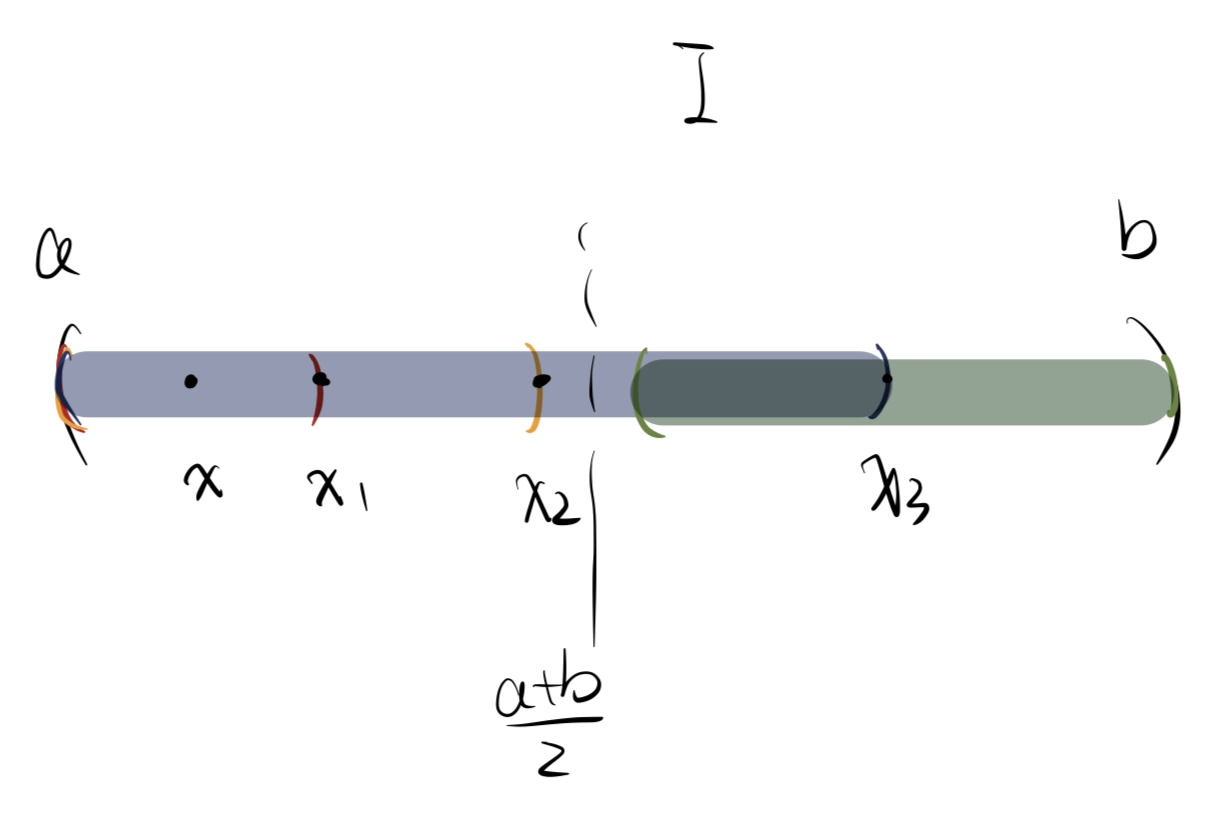
\includegraphics[width=7cm]{attachment/IMG_3538.jpg}
	\caption{\underline{\textbf{证法一}}的示意图, 手绘勿喷}
\end{figure}
	
	\underline{\textbf{证法二}}~~记$\mathcal{E}_x = \{ E \subseteq U: x \in E,E\textit{是开区间} \}$, 令$I_x = \bigcup_{E \in \mathcal{E}_x} E$. 下面证明$I_x \in \mathcal{E}_x$, 从而它就是包含$x$的最大开区间. 
	
	任取$x_1,x_2 \in I_x$, 不妨$x_1<x_2$. 由于存在分别包含$x_1,x_2$的开区间$E_{x_1}, E_{x_2}$, 所以$x_1,x_2 \in E_{x_1} \cup E_{x_2}$. 另一方面, 由于$x \in E_{x_1} \cap E_{x_2}$, $E_{x_1} \cup E_{x_2} \in \mathcal{E}_x$, 进一步$(x_1,x_2) \in \mathcal{E}_x$. 
	
	现在, 记$a = \inf I_x,b = \sup I_x$, 其中$a,b$可以是无穷. 那么对任意$c \in (a,b)$都存在$x_1,x_2$使得$a \leq x_1 < c < x_2 \leq b$, 从而$(a,b) \subseteq I_x \subseteq [a,b]$. 又$I_x$是开集, 可知$I_x = (a,b)$. 
\end{proof}

与开集相对应的概念是所谓闭集. 

\begin{definition}{$\R$上的闭集}
	设$U \subseteq \R$, 称$U$是$\R$上的一个\textit{闭集}(closed set), 如果$\R - U$是开集. 
\end{definition}

一些闭集的例子是: $\R$, $\varnothing$, 任意闭区间, 任意闭区间的交集. 对开集的命题取补集即可得到: 

\begin{proposition}{$\R$上闭集的性质}
	\vspace{-2em}
	\begin{itemize}
		\item $\R,\varnothing$是闭集; 
		\item $\bigcap_{\alpha \in A} U_{\alpha}$是闭集, 其中$U_{\alpha}$是闭集, $A$是指标集; 
		\item $\bigcup_{1 \leq i \leq n} U_i$是闭集, 其中$U_i(i=1,\cdots ,n)$是闭集. 
	\end{itemize}
\end{proposition}
\begin{remark}
	容易举出无限个闭集的并集是开集的例子: 设$I_n = [1+1/n,2-1/n]$, 则$\bigcup_{n\geq 1} I_n = (1,2)$. 
\end{remark}

关于闭集, 一个重要性质是: 

\begin{proposition}{}
	设$U \subseteq \R$, 则$U$是闭集当且仅当$U$的所有聚点都在$U$中. 
\end{proposition}
\begin{proof}
	“$\Rightarrow$”: 设$U$是闭集, 任取$U$的聚点$x$. 假设$x \notin U$, 那么$x \in \R - U$, 从而存在$\varepsilon$使得$x \in B(x,\varepsilon) \subseteq \R - U$, 矛盾. 
	
	“$\Leftarrow$”: 设$U$的任意聚点都在$U$中. 假设$\R - U$不是开集, 即存在$x \notin U$使得任意包含$x$的开球$B(x) \nsubseteq \R - U$即$B(x) \cap U \neq \varnothing$. 选取$x_n \in B(x,1/n) \cap U$可知$x_n \to x$, 矛盾. 
\end{proof}

现在我们给出一个重磅结论: 

\begin{theorem}{($\R$上)连续函数的拓扑表示}
	对于$f:\R \to \R$, $f$是连续函数当且仅当开集的原像是开集, 即对任意的$U\in \tau$, $f^{-1}(U) \in \tau$. 
\end{theorem}
\begin{remark}
	通过取补集的方法, 在此定理的基础上, 我们亦可以证明$f$是连续函数当且仅当闭集的原像是闭集. 
\end{remark}
\begin{proof}
	“$\Rightarrow$”: 任取$x_0 \in f^{-1}(U)$, 记$y_0=f(x_0)$, 存在$\varepsilon$使得对任意$y \in B(y_0,\varepsilon)$都有$y \in U$. 由于$f$连续, 对$\varepsilon$存在$\delta >0$使得对任意$x \in B(x_0,\delta)$都有$|f(x)-y_0|<\varepsilon$, 进而$f(x) \in U$, 说明$x \in f^{-1}(U)$. 
	
	“$\Leftarrow$”: 任取$x_0$, 记$y_0=f(x_0)$, 对任意的$\varepsilon >0$, $f^{-1}(B(y_0, \varepsilon))$是开集, 从而存在$\delta >0$使得$B(x_0,\delta) \subseteq f^{-1}(B(y_0, \varepsilon))$, 这就是说$f(B(x_0,\delta)) \subseteq B(y_0, \varepsilon)$. 
\end{proof}

\begin{figure}[H]
	\centering
	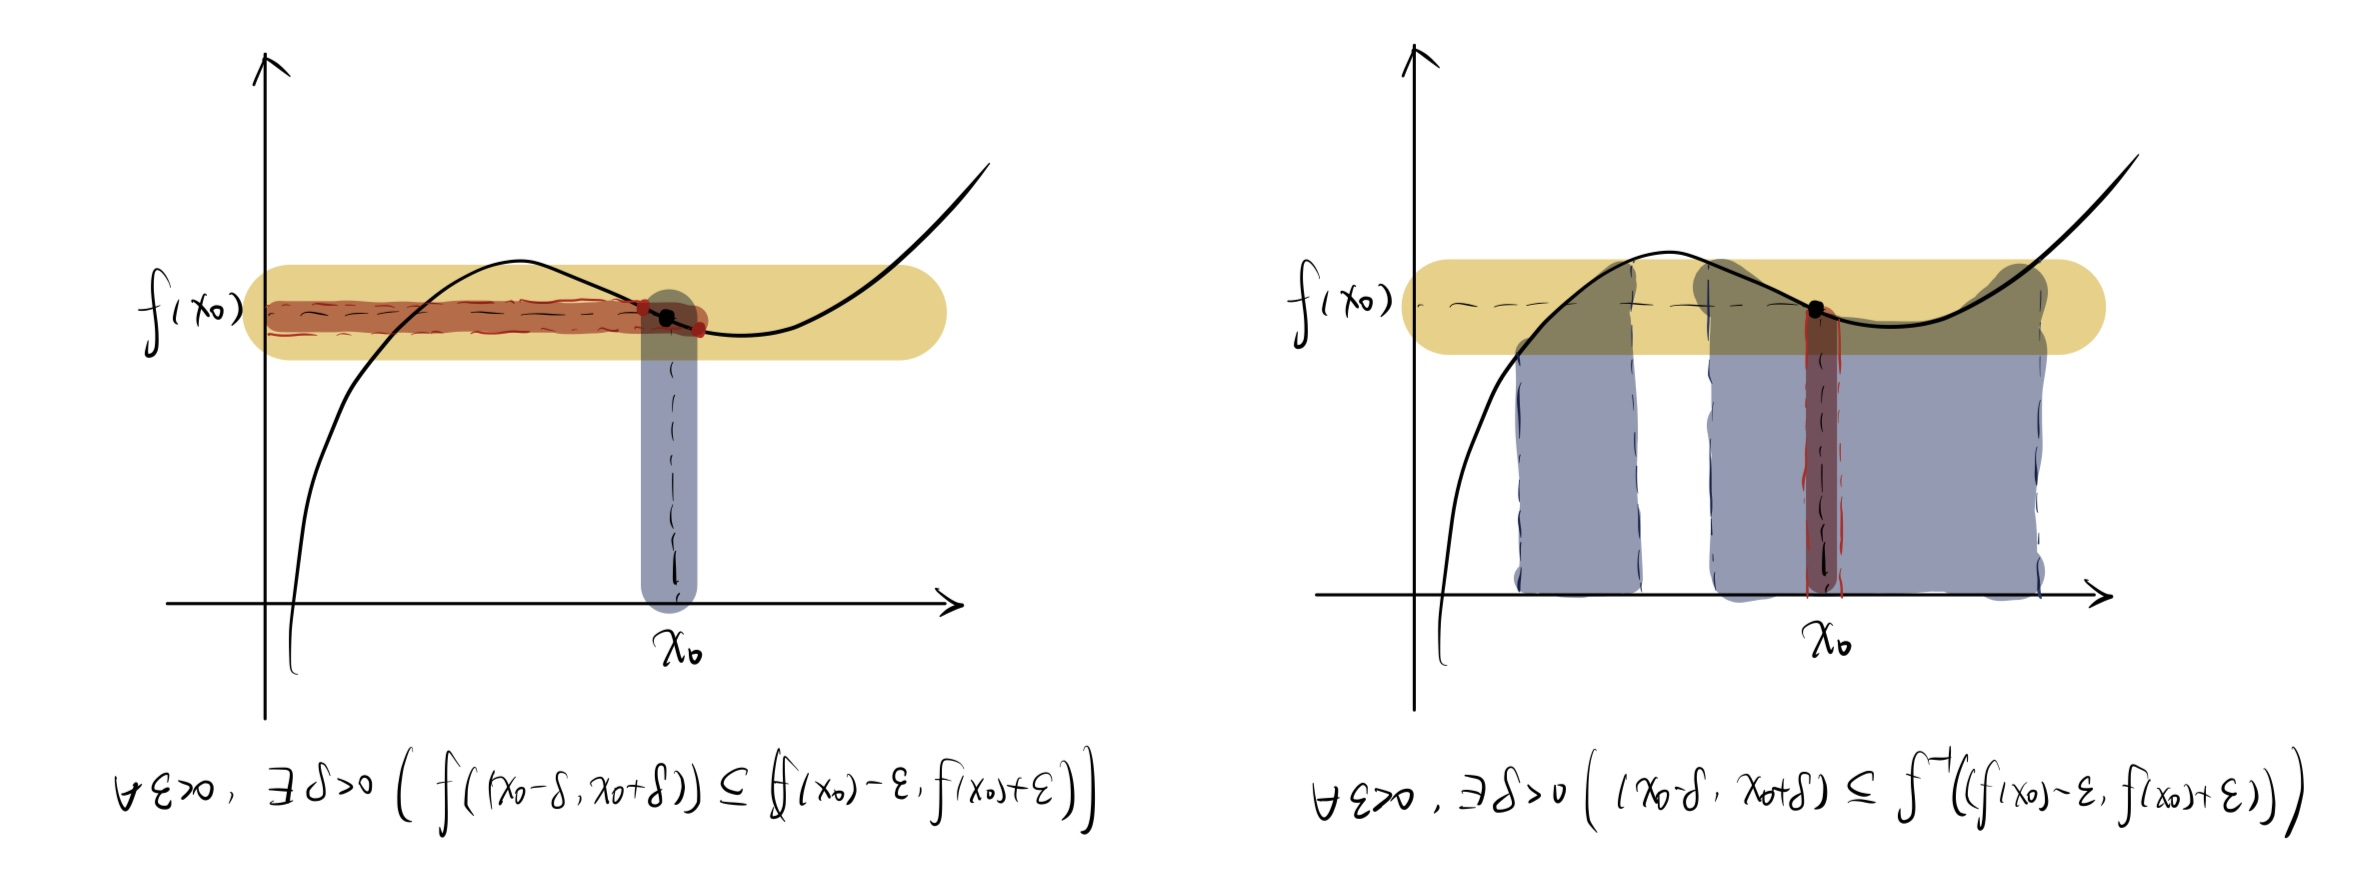
\includegraphics[width=16cm]{attachment/IMG_3539.jpg}
	\caption{两种刻画函数连续性方式的示意图, 手绘勿喷}
\end{figure}

\subsection{拓扑空间}

将开集及其性质抽象出来, 就构成一般的拓扑空间的定义. 

\begin{axiom}{拓扑空间}
	设$X$为非空集合, 称$\tau \in \mathcal{P}(X)$是$X$上的一个\textit{拓扑}(topology), 如果: 
	\begin{itemize}
		\item $X \in \tau$, $\varnothing \in \tau$; 
		\item $\bigcup_{\alpha \in A} U_{\alpha} \in \tau$, 其中$U_{\alpha} \in \tau$, $A$是指标集; 
		\item $\bigcap_{1 \leq i \leq n} U_i \in \tau$, 其中$U_i \in \tau(i=1,\cdots ,n)$. 
	\end{itemize}
	接着, 称$(X,\tau)$是一个\textit{拓扑空间}(topological space), 称$\tau$中的集合为\textit{开集}(open set), 称$U \subseteq X$为\textit{闭集}(closed set)如果$X - U$是开集. 
\end{axiom}

\begin{example}
	设非空集合$X$, 那么
	\begin{itemize}
		\item $\tau = \{ \varnothing ,X\}$称为$X$上的平凡拓扑, 这是$X$上最小的拓扑. 
		\item $\tau = \mathcal{P}(X)$称为$X$上的离散拓扑, 这是$X$上最大的拓扑. 
	\end{itemize}
\end{example}

\begin{definition}{子空间拓扑}
	设拓扑空间$(X,\tau)$, $Y \subseteq X$, 定义$Y$上的拓扑
	\begin{center}
		$\tau _Y := \{ Y \cap U:U \in \tau \}. $
	\end{center}
\end{definition}

类似于$\R$, 我们可以由度量自然地引出拓扑. 

\begin{proposition}{}
	设度量空间$(X,d)$, 称$U \subseteq X$是开集, 如果对任意$x \in U$都存在$\varepsilon >0$使得$B(x,\varepsilon) \subseteq U$. 那么, 由$(X,d)$上开集构成的集合是$X$上的一个拓扑. 
\end{proposition}

\begin{example}
	设非空集合$X$. 
	\begin{itemize}
		\item 拓扑空间不一定都由度量引出, 例如上面例子中的平凡拓扑. 
		\item 定义$d(x,y)= \begin{cases}
 0 &  x=y \\
 1 &  x\neq y
\end{cases}$, 则$d$引出了$X$上的离散拓扑. 
	\end{itemize}
\end{example}
\begin{proof}
	(1) 否则所有开球都要是$X$, 说明$X$上任意两点的距离可以足够小, 进而任意两点间的距离都为$0$, 不满足正定性要求. 
	
	(2) 我们先验证$d$是一个合理的距离函数, 关键在于三角不等式: 设若不然, 即存在$x,y,z \in X$使得$d(x,z)>d(x,y)+d(y,z)$, 那么必然有$d(x,z)=1,d(x,y)=d(y,z)=0$, 矛盾. 
	
	接下来证明其引出离散拓扑, 只要说明对任意$x \in X$, $\{ x \}$是开集. 注意到$\{ x \}=B(x,1/2)$即可. 
\end{proof}

现在来看看一般拓扑空间$(X,\tau)$上和开集和闭集有关的(几何的)概念. 

之前提到过, 在定义$\R$上点列的极限时, 邻域$N_{\varepsilon}(x)$的半径其实不影响最终的敛散性. 另一方面, 拓扑空间上也有可能不存在度量. 因此, 现在有必要将其一般化. 

\begin{definition}{邻域}
	设$x \in X$, 称$A \subseteq X$是$x$的一个\textit{邻域}(neighbourhood), 如果$x \in A \in \tau$. 
\end{definition}

\begin{definition}{导集, 闭包}
	设$A \subseteq X$. 
	\begin{itemize}
		\item 称$x$是$A$的一个\textit{极限点}(limited point), 如果对$x$的任意邻域$U$都有$(U \cap A) - \{ x \} = \varnothing$. 进一步, 称$A$的所有极限点组成的集合为$A$的\textit{导集}(derived set), 记作$A'$. 
		\item 称$x$是$A$的一个\textit{闭包点}(closure point), 如果对$x$的任意邻域$U$都有$U \cap A = \varnothing$. 进一步, 称$A$的所有闭包点组成的集合为$A$的\textit{闭包}(closure), 记作$\overline{A}$. 
	\end{itemize}
\end{definition}
\begin{remark}
	之前在实数章节所定义的聚点, 对应到拓扑空间上就是极限点. 
\end{remark}

容易证明, $A$是闭集当且仅当$A=\overline{A}$(即$A$是闭集当且仅当极限点都在$A$中). 另外, 若$X$在$Y$中稠密, 等价地是说$\overline{X}=Y$. 

\begin{definition}{内部, 外部, 边界}
	设$A \subseteq X$. 
	\begin{itemize}
		\item 称$x$为$A$的\textit{内点}(interior point), 如果存在$x$的一个邻域是$A$的子集. 进一步, 称$A$的所有内点组成的集合为$A$的\textit{内部}(interior), 记作$\Int A$. 
		\item 称$x$为$A$的\textit{外点}(exterior point), 如果$x$是$X-A$的内点. 进一步, 称$A$的所有外点组成的集合为$A$的\textit{外部}(exterior), 记作$\Ext A$. 
		\item 称$x$为$A$的\textit{边界点}(boundary point), 如果$x$既不是$A$的内点也不是$A$的外点. 进一步, 称$A$的所有边界点组成的集合为$A$的\textit{边界}(boundary), 记作$\partial A$. 
	\end{itemize}
\end{definition}

容易证明, $A$是开集当且仅当$A= \Int A$(即$A$是开集当且仅当对任意$x \in A$都存在$U(x) \subseteq A$). 另外, $\overline{A} = \Int A \cup \partial A$(这一点并不显然). 



\newpage
\section{函数列的逐点收敛与一致收敛}

在本节开头必须声明, 函数列的一致收敛性通常会用来研究积分算子, 微分算子, 极限算子与极限算子间的换序问题, 这里只会研究第三种, 其余部分内容会在函数项级数那里补上. 这样安排的目的主要在于为下一章做知识上的铺垫. (顺便还能证明度量空间$\big( C([a,b]),\| \bigcdot \|_{\infty} \big)$的完备性)

\subsection{基本概念}

可以给函数列定义两种收敛方式. 

\begin{definition}{函数列的收敛}
	设度量空间$(X,d)$, $\{ f_n :X \supseteq E \to \R \}_{n\geq 1}$是函数的序列, $f:E \to \R$. 
	\begin{itemize}
		\item 称$f_n$在$E$上\textit{逐点收敛}(pointwisely convergent)到$f$, 记作$f_n \to f,n\to \infty$, 如果对任意的$x \in E$, 数列$f_n(x) \to f(x),n \to \infty$. 
		\item 称$f_n$在$E$上\textit{一致收敛}(uniformly convergent)到$f$, 记作$f_n \rightrightarrows f,n\to \infty$, 如果对任意$\varepsilon >0$都存在$N$使得当$n>N$时对任意$x \in E$都有$|f_n(x)-f(x)|<\varepsilon$. 
	\end{itemize}
\end{definition}
\begin{remark}
	可以注意到, 函数列的极限就像是数列的极限, 我们之后还会将$\mathbb{N} \ni n \to \infty$换成其它基来考虑函数族的收敛性. 
\end{remark}

\begin{example}
	设$f_n(x)=\frac{1}{nx}$, 则在$(0,1)$上$f_n(x)$逐点收敛到$0$, 但并非一致收敛到$0$. 
\end{example}
\begin{proof}
	假设$f_n \rightrightarrows 0$, 即对任意$\varepsilon >0$都存在$N$使得$n>N$时对任意$x \in (0,1)$都有$\frac{1}{nx}<\varepsilon$, 那么$x > \frac{1}{N\varepsilon}$, 显然不可能. 
\end{proof}

\begin{figure}[H]
	\centering
	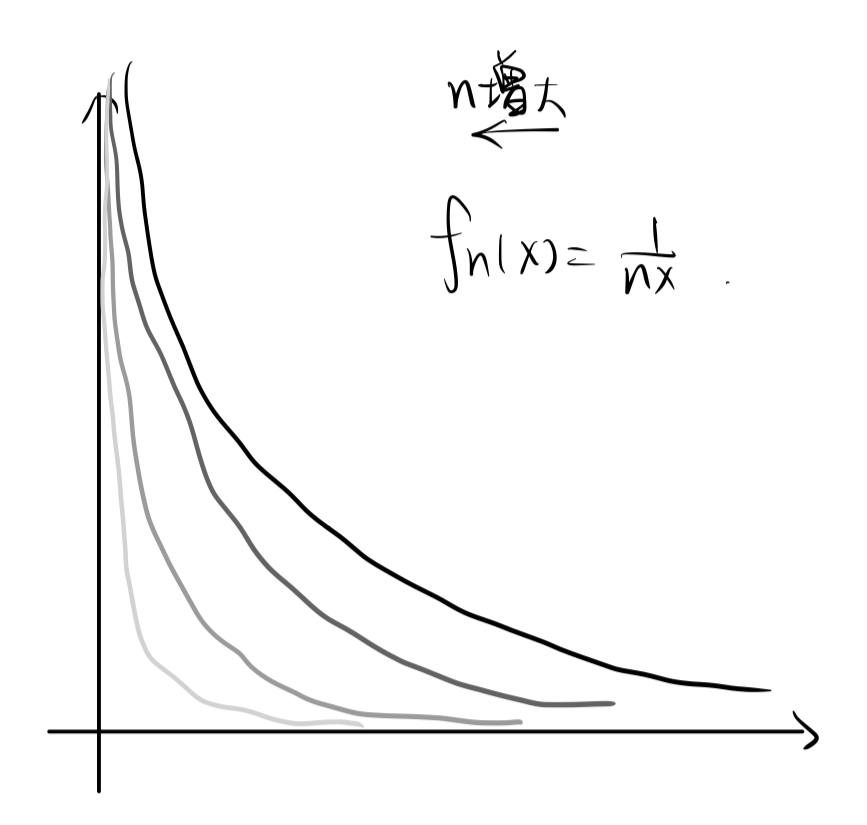
\includegraphics[width=6cm]{attachment/IMG_3545.jpg}
	\caption{$f_n(x)=\frac{1}{nx}$收敛情况的示意图, 手绘勿喷}
\end{figure}

在几何上来看, 若$f_n \rightrightarrows f$, 则对任意$\varepsilon >0$, 对足够大的$n$, $y=f_n(x)$的图像应当完全落在$y=f(x)-\varepsilon$到$y=f(x)+\varepsilon$之间. 

\begin{proposition}{}
	设$E$上的函数列$\{ f_n \}$, 则以下说法等价: 
	
	1) $f_n \rightrightarrows f$;\qquad 2) $\displaystyle \lim_{n\to \infty} \sup_{x \in E}|f_n(x) - f(x)|=0$;\qquad 3) 对任意$\{ x_n \}\subseteq E$都有$f_n(x_n)-f(x_n) \to 0$. 
\end{proposition}
\begin{proof}
	$1) \Rightarrow 2)$和$2) \Rightarrow 3)$都是显然的. 下面证明$3) \Rightarrow 1)$. 
	
	假设$f_n$并非一致收敛于$f$, 即存在$\varepsilon >0$使得有无穷多个$n$满足存在$x_n \in E$使得$|f_n(x_n)-f(x_n)| \geq \varepsilon$, 这就与$3)$矛盾. 
\end{proof}

\begin{example}
	设$f_n(x)=\frac{nx}{1+n^2x^2}$, 则在$(0,+\infty)$上$f_n$并非一致收敛, 在$[\delta ,+\infty )$上一致收敛. 
\end{example}
\begin{proof}
	(1) 显然$f_n \to 0$. 选取$x_n=\frac{1}{n}$, 则$|f_n(\frac{1}{n})-f(\frac{1}{n})| = \frac{1}{2}$, 故$f_n$在$(0,+\infty)$上并非一致收敛. 
	
	(2) 考虑$f_n(x) < \frac{1}{nx} \leq \frac{1}{n\delta}$, 因此$\sup _{x \in [\delta ,+\infty )} |f_n(x)-f(x)| \leq \frac{1}{n\delta}$, 显见其极限为$0$, 因此$f_n$在$[\delta ,+\infty )$上一致收敛到$0$. 
\end{proof}

“在$(0,+\infty)$上并非一致收敛(连续), 而在$[\delta ,+\infty )$上一致收敛(连续)”这种话我们已经见过几次了. 实际上, 我们称$\{ f_n \}$在开集$I$上\textit{内闭一致收敛}(inner closed uniformly convergent), 如果对$I$的任何闭子集$\{ f_n \}$都是一致收敛的. 后面, 我们会见到这一定义的作用. 

类比数列极限, 我们有: 

\begin{theorem}{函数列的Cauchy收敛准则} \label{thm:hjuulpcauchy}
	设$E$上的函数列$\{ f_n \}$, 则$\{ f_n \}$在$E$上一致收敛当且仅当对任意$\varepsilon >0$都存在$N$, 使得对任意$m,n > N$和任意$x \in E$都有$|f_n(x)-f_m(x)|<\varepsilon$. 
\end{theorem}
\begin{proof}
	必要性是显然的. 充分性: 由数列的Cauchy收敛准则可知$\{ f_n \}$在$E$上逐点收敛, 设极限函数为$f$, 在上式中令$m\to \infty$即得$$\forall \varepsilon >0, \exists N \big(\forall n>N,x \in E,  |f_n(x)-f(x)|\leq \varepsilon \big).$$
	这就是说$f_n \rightrightarrows f$. 
\end{proof}

\subsection{极限函数的连续性}

\begin{theorem}{极限函数的连续性} \label{jixmhjuudelmxuxk}
	设$E$上的函数列$\{ f_n \}$, 若对所有$n$都有$f_n$在$E$上连续, 且$f_n \rightrightarrows f$, 则$f$在$E$上连续. 即是说, 
	\begin{center}
		$\displaystyle \lim_{x \to x_0} \lim_{n \to \infty} f_n(x) = \lim_{n\to \infty} \lim_{x \to x_0} f_n(x) , \quad \forall x_0 \in E. $
	\end{center}
\end{theorem}
\begin{remark}
	结合上面的Cauchy收敛准则, 实际上我们可以得到: 由连续函数构成的函数项级数若收敛, 则极限函数连续. 这是构造连续函数的一种重要方式. 
\end{remark}
\begin{proof}
	由一致收敛性, 对任意$\varepsilon >0$, 都存在$N$使得$n>N$时对任意$x \in E$有$|f_n(x)-f(x)|<\frac{\varepsilon}{3}$; 对于$x_0 \in E$, 由$f_n$的连续性可知, 对上方的$\varepsilon$, 存在$\delta$使得当$x \in E \cap B(x_0,\delta)$时$|f_n(x)-f_n(x_0)|<\frac{\varepsilon}{3}$. 
	
	因此, 对$n>N$和$x \in E \cap B(x_0,\delta)$, 我们有$$|f(x)-f(x_0)| \leq |f(x)-f_n(x)|+|f_n(x)-f_n(x_0)| + |f_n(x_0)-f(x_0)| < \frac{\varepsilon}{3} + \frac{\varepsilon}{3} + \frac{\varepsilon}{3} = \varepsilon .$$
	这就是说$f$在$E$上连续. 
\end{proof}

该定理的一个直接推论是: 

\begin{corollary}{}
	若定义在开集$I$上的连续函数列$\{ f_n \}$内闭一致收敛于$f$, 则$f$在$I$上连续. 
\end{corollary}
\begin{proof}
	对任意$x_0 \in I$, 存在$\delta$使得闭球$\{ x:d(x,x_0)\leq \delta \} \subseteq I$, 因此$f$在$x_0$处连续. 
\end{proof}

更一般地: 

\begin{theorem}{Moore-Osgood}
	设$E$上的函数列$\{ f_n \}$, $x_0$是$E$的极限点, 若$\lim_{x \to x_0} f_n(x)$都存在, 记为$a_n$, 且$f_n \rightrightarrows f$, 则$\{ a_n \}$收敛并且$$\lim_{x \to x_0} f(x) = \lim_{n \to \infty} a_n.$$
\end{theorem}
\begin{proof}
	只证明$\{ a_n \}$收敛, 剩下操作和上个定理是几乎一样的. 
	
	由一致收敛性, 对任意$\varepsilon >0$, 存在$N$使得对任意$m,n >N$都有$|f_m(x)-f_n(x)|<\varepsilon$. 在上式中令$x \to x_0$即得$|a_m-a_n|\leq \varepsilon$, 从而$\{ a_n \}$收敛. 
\end{proof}

在阐述下面的定理之前, 我们要将$\R$上闭区间的紧性推广到度量空间上的紧集. 至于紧集有何作用, 我们会在下一章介绍. 

\begin{definition}{开覆盖, 紧集}
	设度量空间$(X,d)$, $S \subseteq X$. 
	\begin{itemize}
		\item 称集合族$\mathcal{U} = \{ U_{\alpha} \}_{\alpha \in A}$为$S$的一个\textit{开覆盖}(open cover), 如果$S \subseteq \bigcup_{\alpha \in A} U_{\alpha}$. 
		\item 承上述定义, 设指标集$A' \subseteq A$, 称$\mathcal{U}$的子集$\mathcal{U}'= \{ U_{\alpha} \}_{\alpha \in A'}$是$U$的\textit{子覆盖}(subcover), 如果$S \subseteq \bigcup_{\alpha \in A'} U_{\alpha}$. 
		\item 称$S$是\textit{紧集}(compact set), 如果$S$的任意开覆盖都存在一个有限子覆盖. 
	\end{itemize}
\end{definition}

\begin{theorem}{Dini}
	设紧集$E$上的函数列$\{ f_n \}$. 若满足: 
	
	1) 极限函数$f$存在且在$E$上连续;\qquad 2) 对每个$n$, $f_n$在$E$上连续;
	
	3) 对任意$x \in E$, $f_n(x)$单调不减收敛到$f(x)$. 
	
	\noindent
	则$f_n \rightrightarrows f$. 
\end{theorem}
\begin{remark}
	单调不增情况是一样的. 
\end{remark}
\begin{proof}
	任意取$\varepsilon >0$. 对$x_0 \in E$, 存在$N(x_0)$使得对$n>N(x_0)$有$0 \leq f(x)-f_{n}(x_0) < \varepsilon$. 由$f,f_n$的连续性可知存在$\delta (x_0)$使得对任意$x \in B(x_0,\delta (x_0))$都有$0 \leq f(x)-f_{n} < \varepsilon$. 
	
	当$x_k$取遍$E$时, $\bigcup_{k\geq 0}B(x_k,\delta (x_k))$构成$E$的开覆盖, 因此存在$K$使得(不妨)$\bigcup_{k=0}^{K}B(x_k,\delta (x_k)) \supseteq E$. 现在取$N_\varepsilon = \max \{ N(x_0),\cdots ,N(x_K) \}$, 那么当$n>N_\varepsilon$时, 对任意$x \in E$都有$0 \leq f(x) - f_n(x) < \varepsilon$. 
\end{proof}


\subsection{相关问题}

\circled{A}~~度量空间$\big( C([a,b]),\| \bigcdot \|_{\infty} \big)$的完备性: 

在以下讨论中, 我们定义函数的一致范数$$\| \bigcdot \|_{\infty} : C([a,b]) \to \R _{\geq 0}, \quad f \mapsto \sup_{x \in [a,b]}|f(x)|. $$
由于$|f(x)|$是$[a,b]$上的连续函数, 可知其有界, 说明$\sup_{x \in [a,b]}|f(x)|$存在, 即$\| f \|$是良定义的. 

\begin{theorem}{}
	$\big( C([a,b]),\| \bigcdot \|_{\infty} \big)$是完备的赋范向量空间. 
\end{theorem}
\begin{proof}
	这是定理\ref{thm:hjuulpcauchy}和定理\ref{jixmhjuudelmxuxk}的直接结论. 
\end{proof}

\circled{B}~~平面填充曲线: 这里以Peano曲线为例. 

记$I=[0,1],E=I^2$. 按如下方式构造一条曲线$f:I \to E$. 先将$E$九等分, 画出每个小格子的对角线, 记该曲线为$f_1$; 再将小格子视作$I$, 重复九等分的构造, 记新的曲线为$f_2$. 如此递归, 得到连续映射$f_n:I \to E$. 

\begin{figure}[H]
	\centering
	\begin{minipage}[t]{0.3\textwidth}
		\centering
		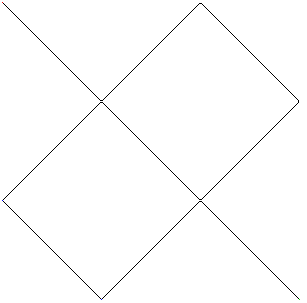
\includegraphics[width=3cm]{attachment/Peano_1.png}
	\end{minipage}
	$\longrightarrow$
	\begin{minipage}[t]{0.3\textwidth}
		\centering
		
\includegraphics[width=3cm]{attachment/Peano_2.png}
	\end{minipage}
	\caption{Peano曲线构造示意图, 图源Wikipedia}
\end{figure}

现在来验证$\{ f_n \}$存在极限$f$. 实际上, 取$N>0$, 对任意的$m,n \geq N$和任意$x \in I$, $f_n(x)$和$f_m(x)$在同一个边长为$3^{-N}$的格子里, 也即$|f_n(x)-f_m(x)| \leq \sqrt{2} \cdot 3^{-N}$. 由Cauchy收敛准则不难得到$f_n \rightrightarrows f$. 特别地, $f$是连续映射. 

Peano曲线$f$可以“填满”区域$E$: 实际上, 对任意$p \in E$, 存在$x$使得$p$和$f_n(x)$的距离不超过$\sqrt{2} \cdot 3^{-n}$, 由$f$的定义可知$f(I)$在$E$中稠密. 另外, 由于$I$是紧集, 故$f(I)$也是紧集, 从而是有界闭集, 结合稠密性可得$f(I)=E$. 


























\chapter{收敛性和连续性的一般化}

在第四章研究函数的连续性时, 我们已经“顺带”定义好了度量空间, 甚至定义了($\R$上)开集, 闭集, 连续映射等拓扑概念. 但是, 有一些微妙的事情我们还没有处理. 例如, 我们说闭区间上连续函数的性质可以推广到所谓“连通的”或者“紧的”集合上; 另外, 我们好奇拓扑空间的具体性质. 这些事情统统可以归在点集拓扑学里, 也就是本章会(部分地)研究的对象. 

事实上本章的内容应该对应Zorich的第七章和第九章. 这样安排的原因主要在于, 连续函数(映射)自然会牵涉到很多拓扑的内容, 紧接着第四章讲拓扑有助于贯通理解这两个概念的关系(而且拓扑和后面的内容没有必要的先后关系). 

本章的核心内容如下表所示. 

\begin{table}[h]
	\small 
	\centering
	\renewcommand\arraystretch{1.4}
	\begin{tabular}{|l|l|p{2cm}|l|p{2cm}|}
	\hline
\multicolumn{1}{|l|}{{ 分类}}       & { 性质}                    & { $\R ^n$或有限维赋范向量空间} & { (一般的)度量空间} & (一般的)拓扑空间        \\ \hline
{ }                             & { 邻域}                    & { 与度量相关}                                          & { 与度量相关}     & 与度量无关            \\ 
\multirow{-2}{*}{{ 度量相关}}       & { 有界性}                   & { 有}                                              & { 有}         & 无                \\ \hline
{ }                             & { 点列极限的性质}               & { 极限唯一; 点列有界}                                      & { 极限唯一; 点列有界} & Hausdorff空间中极限唯一 \\
{ }                             & { 点列极限线性运算法则}            & { 有}                                              & { 无}         & 无                \\
\multirow{-3}{*}{{ 点列的极限}}      & { 点列极限按分量收敛性质}           & { 有}                                              & { /}         & /                \\ \hline
{ }                             & { Cauchy收敛准则}            & { 有(利用上一条证明)}                                     & { 对应完备性}     & 无                \\
{ }                             & { 闭区间套定理}             & { {闭集套定理}}                                        & { 闭球套定理, 紧集套定理} & 紧集套定理            \\
{ }                             & { Bolzano-Weierstrass定理} & { 有}                                              & { 对应列紧性}     & 对应列紧性            \\ 
\multirow{-4}{*}{{ 实数完备性定理的推广}} & { Heine-Borel定理}         & { 有}                                              & { 对应紧致性}     & 对应紧致性            \\ \hline
{ }                             & { 函数极限的性质}             & { 极限唯一; 最终有界}                                              & { 极限唯一; 最终有界}         & /                \\ 
{ }                             & { Heine归结原理}             & { 有}                                              & { 有}         & /                \\ 
{ }                             & { 函数极限运算法则}              & { 有}                                              & { 有}         & /                \\
{ }                             & { 函数的Cauchy收敛准则}         & { 有}                                              & { 有}         & /                \\
{ }                             & { Cantor-Heine的一致连续性定理}  & { 有}                                              & { 如果定义域是紧集}  & /                \\
\multirow{-5}{*}{{ 函数/映射的极限}}   & Weierstrass最大值定理                             & 有                                                                     & 无                                & /  \\ \hline              
\end{tabular}
\caption{$\R ^n$, 度量空间, 拓扑空间有关收敛性和连续性的性质对比}
\end{table}

\section{$\R ^n$上的点列极限与连续映射}

在$\R ^n$中, 我们定义开球(邻域)$B(x_0,\varepsilon)$为$\{ x \in X:d(x,x_0)<\varepsilon \}$, 其中$d$是由范数$\| (x^1,\cdots ,x^n) \| = \sqrt{(x^1)^2+\cdots (x^n)^2}$引出的度量. 称点列$\{ x_k \}$是有界的, 如果存在$M>0$使得对任意$k$都有$\| x_k \|<M$. 

\subsection{点列的极限}

\begin{definition}{点列的极限}
	称点$l \in \R ^n$为点列$\{ x_k \}$的\textit{极限}(limit), 如果对任意的$l$的邻域$B(l,\varepsilon)$都存在$N$使得当$k \geq N$时$x_k \in B(l,\varepsilon)$. 记为$$l = \lim_{k \to \infty} x_k ~~ \text{或} ~~ x_k \to l,~k \to \infty$$且称$\{ x_k \}$\textit{收敛}(convergent)于$l$. 
\end{definition}

\begin{proposition}{点列极限的性质}
	(1) 收敛点列存在唯一的极限. \qquad (2) 收敛点列必有界. \\
	(3) 点列收敛于一点当且仅当其所有子列都收敛于同一点. 
\end{proposition}

\begin{proposition}{点列极限线性运算法则}
	设$\R ^n$中收敛点列$\{ x_k \},\{ y_k \}$, 收敛的实数列$\{ l_n \}$, 则
	
	(1) $\lim_{k\to \infty} (x_k+y_k) = \lim_{k\to \infty} x_k + \lim_{k\to \infty} y_k$. 
	
	(2) $\lim_{k\to \infty} (l_kx_k) = \lim_{k\to \infty} l_k \lim_{k\to \infty} x_k$. 
\end{proposition}

由于$\R ^n$上没有序结构, 夹逼定理, 保序性等性质无法推广. 

\begin{lemma}{点列极限按分量收敛}
	设$\R ^n$中的点列$x_k = (x^1_k, \cdots ,x_k^n)$和点$l=(l^1,\cdots ,l^n)$, 则$$\lim_{k\to \infty} x_k = l \Longleftrightarrow \lim_{k\to \infty} x^i_k = l^i,~~i=1,\cdots ,n. $$
\end{lemma}
\begin{proof}
	利用下方不等式控制即可$$\max_{1 \leq i \leq n} |x^i_k-l^i| \leq \| x_k-l \| \leq \sum_{i=1}^{n} |x^i_k-l^i|. $$
\end{proof}

\subsection{实数完备性定理的推广}

\begin{definition}{Cauchy列}
	一个点列$\{ x_k \}$被称作\textit{Cauchy列}(Cauchy sequence),如果对于任意的$\varepsilon >0$都存在自然数$N$使得$\| x_k-x_p \|<\varepsilon$对$k,p>N$恒成立.
\end{definition}

\begin{theorem}{$\R ^n$中的Cauchy收敛准则}
	一个点列收敛当且仅当它是一个Cauchy列.
\end{theorem}
\begin{remark}
	这说明$\R ^n$是Banach空间. 
\end{remark}
\begin{proof}
	必要性显然. 充分性: 由于不等式$|x^i_k - x^i_p| \leq \| x_k - x_p \|(i=1,\cdots ,n)$, 可知$\{ x^1_k \},\cdots ,\{ x^n_k \}$都是Cauchy列, 由实数列的Cauchy收敛准则知它们都收敛, 从而$\lim_{k\to \infty} x_k = (\lim_{k\to \infty} x^1_k,\cdots , \lim_{k\to \infty} x^n_k)$. 
\end{proof}

我们定义集合$X \subseteq \R ^n$的直径如下: $$\diam X := \sup_{x,y \in X} \| x-y \|. $$

\begin{theorem}{闭集套定理}
	设$\R ^n$中的非空闭集列$\{ F_k \}$. 若$F_1 \supseteq \cdots \supseteq F_k \supseteq \cdots$且$\lim_{k\to \infty} \diam F_k=0$, 则存在唯一的$c \in \R ^n$使得$c \in \bigcap_{k\geq 1} F_k$. 
\end{theorem}
\begin{proof}
	存在性: 在每个$F_k$中取点$x_k$, 从而$\{ x_N,x_{N+1},\cdots \} \subseteq F_N$, 所以$\| x_{k}-x_p \| \leq \diam F_N \to 0, N\to \infty$对所有$k,p >N$成立. 进一步, $\{ x_k \}$是Cauchy列, 设其极限为$c$, 由于所有$F_k$都是闭集, 可知$c \in F_k,k\geq 1$. 
	
	唯一性: 假设存在$c_1,c_2 \in \bigcap_{k\geq 1} F_k$, 可知$\| c_1-c_2 \| \leq \diam F_k \to 0, k\to \infty$, 从而$c_1=c_2$. 
\end{proof}

\begin{theorem}{Bolzano-Weierstrass}
	$\R ^n$中的有界点列一定有收敛子列. 
\end{theorem}
\begin{proof}
	设点列$\{ x_k \}$有界, 则每个坐标组成的数列$\{ x^i_k \}$均有界. 归纳地操作: 在第$i+1$个数列中按照下标$m_{{i,k}}$选出有界数列, 再在其中选取收敛子列$\{ x^{i+1}_{m_{i+1,k}} \}$. 从而$\{ x_{m_{n,k}} \}$是$\{ x_k \}$的收敛子列. 
\end{proof}

\begin{theorem}{Heine-Borel}
	设$X \subseteq \R ^n$, 若$X$是有界闭集, 则任意$X$的开覆盖都存在有限子覆盖. 
\end{theorem}
\begin{proof}
	我们将证明留到拓扑不变量一节说明. 
\end{proof}

\subsection{多元函数的重极限}

对于一般定义的向量值函数$f:\R ^n \supseteq X \to \R ^n$, 我们可以将其分解为$f=(f^1,\cdots ,f^m)$, 因此只需研究值域为$\R$的函数, 称为多元函数. 

\begin{definition}{多元函数的重极限}
	设$f: \R ^n \supseteq X \to \R$, $\mathcal{B}$是$X$上的基. 称$l$为函数$f$\textit{在基$\mathcal{B}$上的极限}, 如果对于$l \in \R$的任何邻域$B(l,\varepsilon)$都存在$B \in \mathcal{B}$使得$f(B) \subseteq B(l,\varepsilon)$. 记作
	\begin{center}
		$\displaystyle \lim_{\mathcal{B}}f(x)=l.$
	\end{center}
\end{definition}

\begin{proposition}{多元函数极限的性质}
	(1) 收敛的多元函数存在唯一的极限. \qquad (2) 在$\mathcal{B}$上收敛的多元函数在$\mathcal{B}$上最终有界. 
\end{proposition}

只要证明Heine归结原理, 剩下的函数极限性质都能自然推出. 

\begin{theorem}{多元函数的Heine归结原理}
	设$f: \R ^n \supseteq X \to \R$, $x_0$是$X$的一个极限点, 则$\lim_{x\to \x_0}f(x)=l$当且仅当对于任意收敛于$x_0$的点列$\{ x_k \} \in X$都有$\lim_{k\to \infty} f(x_k)=l$. 
\end{theorem}
\begin{proof}
	必要性由定义是显然的. 充分性: 用反证法. 假设$f$在$x_0$处的极限不为$l$, 则存在$B(l,\varepsilon)$使得对任意的正整数$k$, 存在$x_k \in B(x_0,1/k)$使得$f(x_k) \notin B(l,\varepsilon)$. 所有这样的$x_k$构成一个收敛于$x_0$的数列, 但不符合题目条件, 即得矛盾. 
\end{proof}

利用Heine归结原理, 容易说明$f(x,y)$分别对$x,y$连续不一定能得到$f$对$(x,y)$连续. (至于何时是一定能得到的, 我们会在下一小节给出)

\begin{example}
	设函数$f(x,y) = \begin{cases}
 \frac{xy}{x^2+y^2} &  (x,y) \neq (0,0) \\
 0 &  (x,y) = (0,0)
\end{cases}$. 显然$f$对两个变量分别连续, 说明$f$对$(x,y)$不连续. 
\end{example}
\begin{proof}
	考虑收敛到$(0,0)$的点列$\{ \frac{1}{k}(1,\lambda) \}$, 但是$f(\frac{1}{k}(1,\lambda)) \to \frac{\lambda}{1+\lambda ^2} \neq 0$, 说明$f$在$(0,0)$处不连续. 或者, 注意到对$f(a,a) \equiv \frac{1}{2}, a \neq 0$. 
\end{proof}

\begin{theorem}{多元函数极限的算术运算}
	设函数$f:\R ^n \supseteq X \to \R, g:X \to \R$, $\mathcal{B}$是$X$上的基. 记$\lim_{\mathcal{B}} f(x) = A, \lim_{\mathcal{B}} g(x) = B$. 
	
	a) 加减法. $\lim_{\mathcal{B}} (f\pm g)(x) = A\pm B.$
	
	b) 乘法. $\lim_{\mathcal{B}} (f\cdot g)(x) = A \cdot B.$
	
	c) 除法, 其中$B\neq 0$. $\lim_{\mathcal{B}} \ssb{\frac{f}{g}}(x) = \frac{A}{B}.$
\end{theorem}

\begin{theorem}{多元函数极限的Cauchy收敛准则}
	设函数$f:\R ^n \supseteq X \to \R$, $\mathcal{B}$是$X$上的基, 则$f$在$\mathcal{B}$上存在极限当且仅当对任意$\varepsilon >0$都存在$B \in \mathcal{B}$使得任意$x,y \in B$有$|f(x)-f(y)|<\varepsilon$. 
\end{theorem}

\begin{theorem}{多元函数复合的极限}
	设一元函数$f$和$n$元函数$g$, 若$\lim_{y\to y_0} f(y)=l, \lim_{x \to x_0}g(x) = y_0$且存在$r$使得$0 \notin g(B(x_0,r))$, 则$\lim_{x \to x_0} f(g(x)) = l$. 
\end{theorem}
\begin{remark}
	这个定理不用基的形式写是为了直观考虑, 实际上对任意基都是成立的. 
\end{remark}

\subsection{多元函数的累次极限}

相对于重极限, 多元函数的累次极限将每个变量逐个取极限而不是同时取极限. 容易发现, 我们只需要研究二元函数的累次极限就足够了. 

正如上一小节例题所述, 累次极限不一定等于重极限. 而且, 不同次序的累次极限也不一定相等. 一般地, 我们有如下的两个条件: 

\begin{proposition}{}
	设二元函数$f:\R ^2 \supseteq X \to \R$, $(x_0,y_0)$是$X$的一个极限点. 若$x \to x_0$时$f(x,y)$一致收敛, $y \to y_0$时$f(x,y)$逐点收敛, 则$$\lim_{y\to y_0} \lim_{x \to x_0} f(x,y) = \lim_{x\to x_0} \lim_{y \to y_0} f(x,y). $$
\end{proposition}
\begin{proof}
	这是Moore-Osgood定理(函数族版本)的直接推论. 
\end{proof}

\begin{proposition}{}
	设二元函数$f:\R ^2 \supseteq X \to \R$, $(x_0,y_0)$是$X$的一个极限点. 若重极限$\lim_{(x,y) \to (x_0,y_0)} f(x,y)$存在, 且对所有$y \neq y_0$, $\lim_{x \to x_0} f(x,y)$存在, 那么$$\lim_{y\to y_0} \lim_{x \to x_0} f(x,y) = \lim_{(x,y) \to (x_0,y_0)} f(x,y).$$
\end{proposition}
\begin{remark}
	反过来就得到重极限不存在的充分条件: 若两种累次极限均存在且不相等, 则重极限一定不存在. 
\end{remark}
\begin{proof}
	由重极限存在可知, 对于任意$\varepsilon >0$, 存在$\delta >0$使得只要$|x-x_0|<\delta,|y-y_0|<\delta$就有$|f(x,y)-l|<\varepsilon$. 对于满足$|y-y_0|<\delta$的$y$, 记$\varphi (y) = \lim_{x \to x_0} f(x,y), y \in (y_0-\delta ,y_0) \cup (y_0,y_0 + \delta)$, 那么在上面的不等式中令$x \to x_0$就有$|\varphi (y) - l | \leq \varepsilon$, 说明$\lim_{y \to y_0} \varphi (y) = l$. 
\end{proof}

以上两条命题说明, 在研究累次极限换序问题时, 应该优先考虑重极限是否存在, 若存在则看单次极限是否逐点收敛, 若不存在则看单次极限是一致收敛还是逐点收敛. 

\begin{example}
	分别计算下列二元函数在$(x,y) \to (0,0)$时的累次极限和二重极限: $$1)~~f(x,y) = xy,\qquad 2)~~f(x,y) = (x+y)\sin \frac{1}{x} \sin \frac{1}{y},\qquad 3)~~f(x,y) = \begin{cases} x+y\sin \frac{1}{x} & x\neq 0 \\ 0 & x=0 \end{cases}, $$
	$$4)~~f(x,y) = \begin{cases} \frac{xy}{x^2+y^2} &  (x,y) \neq (0,0) \\ 0 &  (x,y) = (0,0) \end{cases},\qquad 5)~~f(x,y)=\frac{x-y}{x+y},\qquad 6)~~f(x,y)=\frac{x}{y}. $$
\end{example}

\subsection{多元函数的连续性}

\begin{definition}{多元函数的连续性}
	设$f:\R ^n \supseteq X \to \R$, 若$X \ni x_0$是$X$的一个极限点, 我们称$f$在$x_0$点处\textit{连续}(continuous), 如果$\lim_{X \ni x \to x_0} f(x) = f(x_0)$. 等价地有: 
	\begin{itemize}
		\item 对于任意$\varepsilon >0$, 存在$\delta >0$使得$f(B(x_0,\delta) - \{ x_0 \}) \subseteq B(f(x_0),\varepsilon)$; 
		\item 对任意的点列$\{ x_n \}$, 若$\lim_{n \to \infty} x_n = x_0$, 则$\lim_{n \to \infty} f(x_n) = f(x_0)$. 
	\end{itemize}
\end{definition}
\begin{remark}
	和一元函数连续性的定义类似, 有些书将定义扩大到了$X$的所有点, 而我们可以验证在第一种等价说法下$f$在孤立点处总是连续的. 
\end{remark}

多元函数连续性的基本性质可以由其极限性质直接得到, 请读者参考一元函数连续性章节, 这里不再一一罗列. 

\begin{example}
	设投影算子$\pi _i :\R ^n \to \R ,(x^1,\cdots ,x^n) \mapsto x^i,i=1,\cdots ,n$, 则$\pi _i$在$\R ^n$上连续. 
\end{example}
\begin{proof}
	利用不等式$|f(x)-f(y)|=|x^i - y^i| \leq \| x-y \|$控制即可. 
\end{proof}

类似于上一小节的Moore-Osgood定理, 我们有: 

\begin{proposition}{}
	设$f:\R ^2 \supseteq X \to \R$. 若$f$在$X$上对$x,y$分别连续, 且满足下列两个条件之一, 则$f$在$X$上连续. 
	
	1)~~$f$对某个变量一致连续;\qquad 2)~~$f$对某个变量单调. 
\end{proposition}
\begin{proof}
	(1) 不妨$f$对$x$一致连续. 对任意$\varepsilon _1>0$, 存在$\delta _1 >0$, 对任意$y$, 当$|x_1-x_2|<\delta _1$时$|f(x_1,y)-f(x_2,y)|<\varepsilon _1$; 对任意$\varepsilon _2>0$和任意$x$, 存在$\delta _2 >0$, 当$|y_1-y_2|<\delta _2$时$|f(x,y_1)-f(x,y_2)|<\varepsilon _2$. 所以, 当$\| (x,y)-(x_0,y_0) \|<\min \{ \delta _1,\delta _2 \}$时, $$|f(x,y)-f(x_0,y_0)| \leq |f(x,y)-f(x_0,y)| + |f(x_0,y)-f(x_0,y_0)| < \varepsilon _1 + \varepsilon _2. $$
	
	(2) 不妨$f$对$x$单调. 反过来说, 若能找到控制$|\Delta x| < \delta _0$, 有
	\begin{align*}
		|f(x+\Delta x,y+\Delta y)-f(x,y)| &\leq |f(x+\Delta x,y+\Delta y) - f(x+\Delta x,y)| + |f(x+\Delta x,y) - f(x,y)|  \\
		&\leq \max \{ |f(x \pm \delta _0 , y+\Delta y) - f(x \pm \delta _0 , y)| + |f(x \pm \delta _0 , y) - f(x,y)| \}.
	\end{align*}
	实际上, 重复(1)的过程, 我们令$\delta _0 = \min \{ \delta _1,\delta _2 \}$即可. 细节留给不放心的读者自行验证. 
\end{proof}

由于$\R ^n$是度量空间, 函数连续的拓扑表示自然是成立的. 

\subsection{有界闭集上连续函数的性质}

我们可以定义多元函数的一致连续. 

\begin{definition}{多元函数的一致连续性}
	设$f:\R ^n \supseteq X \to \R$, 称$f$在$X$上\textit{一致连续}(uniformly continuous), 如果对任意$\varepsilon >0$都存在$\delta >0$使得对任意$x,y \in X$, 只要$\| x-y \|<\delta$就有$|f(x)-f(y)|<\varepsilon$. 
\end{definition}

\begin{theorem}{Cantor-Heine的一致连续性定理}
	设$f:\R ^n \supseteq X \to \R$. 若$X$是有界闭集, 则$f$在$X$上连续. 
\end{theorem}
\begin{proof}
	重复一元函数对应定理中利用Bolzano-Weierstrass证明的部分即可. 
\end{proof}

\begin{theorem}{Weierstrass最大值定理}
	设$f:\R ^n \supseteq X \to \R$. 若$X$是有界闭集, 则$f$在$X$上有界且能取到极值. 
\end{theorem}
\begin{proof}
	重复一元函数对应定理中利用Bolzano-Weierstrass证明的部分即可. 
\end{proof}

现在来补上之前缺少的一个证明: 

\begin{proposition}{}
	$n$维向量空间$V$上的所有范数都等价. 
\end{proposition}
\begin{proof}
	取$V$的一组基$v_1,\cdots ,v_n$. 设$x=(x^1,\cdots ,x^n)$, 定义$\| x \| = \sqrt{\sum_{j=1}^{n} (x^j)^2}$. 设另一个范数$N(\bigcdot )$, 下证$N(\bigcdot )$和$\| \bigcdot \|$等价. 
	
	先证明$N$是范数$\| \bigcdot \|$下的连续函数. 任取$x=(x^1,\cdots ,x^n),y=(y^1,\cdots ,y^n)$. 由范数的三角不等式可知$|N(x)-N(y)| \leq N(x-y)$, 从而
	\begin{align*}
		|N(x)-N(y)| &\leq N(x-y) = N\left( \sum_{j=1}^{n} (x^j-y^j)v_j \right) \leq \sum_{j=1}^{n} (x^j-y^j)N(v_j) \\
		&\leq \sqrt{\sum_{j=1}^{n} (x^i-y^i)^2} \cdot \sqrt{\sum_{j=1}^{n} (N(v_j))^2} = C\| x-y \|. 
	\end{align*}
	
	接着, 考虑$V$中的欧氏单位球面$S=\{ x \in V:\| x \|=1 \}$, 显然$S$是有界闭集, 从而$N$在$S$上可以取到最大值$M$和最小值$m(>0)$. 对任意非零的$x \in V$有$\frac{x}{\| x \|} \in S$, 所以$m \leq N(\frac{x}{\| x \|}) \leq M$, 这就是说$m\| x \| \leq N(x) \leq M\| x \|$. 
\end{proof}


\newpage
\section{度量空间上的点列极限与连续映射}

这里我们讨论一般度量空间$(X,d)$, 因此极限算子的线性运算性质就没有了. 除此之外, $(X,d)$和$\R ^n$很多性质是相同的(但是证明方法不同). 

此处我们定义开球$B(x_0,\varepsilon) = \{ x\in X:d(x,x_0)<\varepsilon \}$. 定义集合$E$的直径$\diam E := \sup_{x,y \in E}d(x,y)$. 称集合$E$有界, 若$\diam E \in \R$. 

\subsection{点列的极限}

\begin{definition}{点列的极限}
	称点$l \in X$为点列$\{ x_k \}$的\textit{极限}(limit), 如果对任意的$l$的邻域$B(l,\varepsilon)$都存在$N$使得当$k \geq N$时$x_k \in B(l,\varepsilon)$. 记为$$l = \lim_{k \to \infty} x_k ~~ \text{或} ~~ x_k \to l,~k \to \infty$$且称$\{ x_k \}$\textit{收敛}(convergent)于$l$. 
\end{definition}

\begin{proposition}{点列极限的性质}
	(1) 收敛点列存在唯一的极限. \qquad (2) 收敛点列必有界. \\
	(3) 点列收敛于一点当且仅当其所有子列都收敛于同一点. 
\end{proposition}

\subsection{实数完备性定理的推广}

在$(X,d)$中, 完备性定理都变成了拓扑性质的定义(或推论), 我们会在拓扑不变量一节中深入研究和有界闭性, 紧性, 列紧性的相关内容, 这里只看一个和完备性相关的定理. 

在下面的定理中, 定义闭球为$\tilde{B}(x_0,\varepsilon):=\{ x:d(x,x_0)\leq \varepsilon \}$. 

\begin{theorem}{闭球套定理}
	设度量空间$(X,d)$, 闭球套$\tilde{B}(x_1,r_1) \supseteq \cdots \supseteq \tilde{B}(x_n,r_n) \supseteq \cdots$. 若$r_n \to 0,n\to \infty$, 则$(X,d)$完备当且仅当存在唯一的同时属于每个闭球的点. 
\end{theorem}
\begin{proof}
	(1) 必要性. 设$(X,d)$完备, 先证明球心点列$\{ x_n \}$是Cauchy列: 实际上, 由$r_n \to 0,n\to \infty$可知对任意$\varepsilon >0$存在$N$使得对任意$n >N$都有$r_n<\frac{\varepsilon}{2}$, 从而对任意$m,n>N$, $x_m,x_n \in \tilde{B}(x_N,r_N)$, 那么$$d(x_m,x_n) \leq d(x_m,x_N)+d(x_N,x_n) < \frac{\varepsilon}{2} + \frac{\varepsilon}{2} = \varepsilon .$$
	于是$\{ x_n \}$存在极限$x \in X$. 另一方面, 任意取定$N$, 则对任意$n>N$都有$x_n \in \tilde{B}(x_N,r_N)$. 取$n$使得$d(x_N,x_n) \neq r_N$(存在这样的$n$, 否则显然$r_n \nrightarrow 0$, 矛盾), 由$x_n \to x$可知存在$M$使得当$m>M$时$d(x_m,x)<r_N-d(x_N,x_n)$. 注意到若$n_1>n_2$则$d(x_N,x_{n_1}) \leq d(x_N,x_{n_2})$, 因此只要令$m>\max \{ M,n \}$就有$d(x_m,x)<r_N-d(x_N,x_n)<r_N-d(x_N,x_m)$, 从而$$d(x,x_N) \leq d(x,x_m) + d(x_m,x_N) < r_N. $$
	这说明对任意$N$都有$x \in \tilde{B}(x_N,r_N)$. 
	
	(2) 充分性: 设$\{ x_n \}$是Cauchy列, 则对任意$k$, 存在$N_k$使得对任意$m,n>N_k$有$d(x_n,x_m)<a_k$, 这里$\{ a_k \}$是待定的单减数列, 因此不妨让$\{ N_k \}$是单增数列. 构造$\tilde{B}(x_{N_k},b_k)$, 任取$x \in \tilde{B}(x_{N_{k+1}},b_{k+1})$可知$$d(x,x_{N_k}) \leq d(x,x_{N_{k+1}}) + d(x_{N_{k+1}}, x_{N_{k}}) < a_{k+1}+a_k < 2a_k. $$
	因此只需取$a_k=\frac{1}{2^{k+1}}, b_k = \frac{1}{2^k}$就能保证$\tilde{B}(x_{N_k},b_k)$可以构成闭球套. 
	
	由假设可知, 存在唯一的$x \in \bigcap_{k\geq 1} \tilde{B}(x_{N_k},b_k)$. 由于$d(x,x_{N_k})<a_k\to 0$, $\{ x_n \}$的一个子列$\{ x_{N_k} \}$收敛于$x$, 从而$x_n \to x, n\to \infty$. 
\end{proof}

\subsection{映射的极限与连续性}

\begin{definition}{映射的极限}
	设$f: X \supseteq E \to Y$, $\mathcal{B}$是$E$上的基. 称点$l$为映射$f$\textit{在基$\mathcal{B}$上的极限}, 如果对于$l \in Y$的任何邻域$B(l,\varepsilon)$都存在$B \in \mathcal{B}$使得$f(B) \subseteq B(l,\varepsilon)$. 记作
	\begin{center}
		$\displaystyle \lim_{\mathcal{B}}f(x)=l.$
	\end{center}
\end{definition}

\begin{proposition}{映射极限的性质}
	(1) 收敛的映射存在唯一的极限. \qquad (2) 在$\mathcal{B}$上收敛的映射在$\mathcal{B}$上最终有界. 
\end{proposition}

容易证明, Heine归结原理对于度量空间上的映射也是成立的, 因此可得映射极限的算术运算规则和Cauchy收敛准则. 另外由定义还可以直接得到复合映射的极限(和连续性)定理. 

\begin{definition}{极限的连续性}
	设$f:X \supseteq E \to Y$, 若$E \ni x_0$是$E$的一个极限点, 我们称$f$在$x_0$点处\textit{连续}(continuous), 如果$\lim_{E \ni x \to x_0} f(x) = f(x_0)$. 等价地有: 
	\begin{itemize}
		\item 对于任意$\varepsilon >0$, 存在$\delta >0$使得$f(B(x_0,\delta) - \{ x_0 \}) \subseteq B(f(x_0),\varepsilon)$; 
		\item 对任意的点列$\{ x_n \}$, 若$\lim_{n \to \infty} x_n = x_0$, 则$\lim_{n \to \infty} f(x_n) = f(x_0)$. 
	\end{itemize}
\end{definition}

关于有界闭集上连续映射的性质, 因为有界闭性既不能得到紧性也不能得到列紧性, 因此\textit{Cantor-Heine的一致连续性定理}和\textit{Weierstrass最大值定理}都无从谈起(但分别在紧集和列紧集上是适用的). 



\newpage
\section{拓扑空间上的点列极限与连续映射}

\subsection{拓扑空间中点列的收敛性}

\begin{definition}{点列的极限}
	称点$l \in X$和点列$\{ x_k \}$. 如果对任意的$l$的邻域$U(l)$都存在$N$使得当$k \geq N$时$x_k \in U(l)$. 称$\{ x_k \}$\textit{收敛}(convergent)于$l$. 
\end{definition}

需要注意的是, 由于拓扑空间中邻域的概念和度量无关, 我们不能直接得到点列极限唯一这一命题. 但如果人为地加上限制条件就可以: 

\begin{axiom}{Hausdorff空间}
	设拓扑空间$(X,\tau)$, 称$X$是一个\textit{Hausdorff空间}(Hausdorff space), 如果对任意$x_1,x_2 \in X$都存在邻域$U(x_1),U(x_2)$使得$U(x_1) \cap U(x_2) = \varnothing$. 
\end{axiom}

由刚才的观察直接可以得到: 

\begin{proposition}{}
	在Hausdorff空间中收敛点列存在唯一极限. 
\end{proposition}

显然度量空间都是Hausdorff空间(这是我们的思想来源). 

Hausdorff空间还有一些值得研究的性质(包括相关的分离性公理), 但对于数分的学习没有太大帮助, 就不提了. 

\subsection{拓扑空间之间的连续映射}

\begin{definition}{拓扑空间之间的连续映射}
	设拓扑空间$(X,\tau _X),(Y,\tau _Y)$, 称$f: X \to Y$是\textit{连续映射}(continuous mapping), 如果对任意$U \in \tau _Y$, $f^{-1}(U) \in \tau _X$. 
\end{definition}

\begin{proposition}{}
	设拓扑空间$(X,\tau _X),(Y,\tau _Y)$, 则$f:X \to Y$是连续映射当且仅当对任意$x \in X$, 任取$f(x)$的邻域$U_Y(f(x))$都存在$x$的邻域$U_X(x)$使得$f(U_X(x)) \subseteq U_Y(f(x))$. 
\end{proposition}

类似地, 深入研究拓扑空间之间的连续映射是点集拓扑学的任务, 我们暂时略去. 


\newpage
\section{拓扑不变量}

先定义同胚的概念: 

\begin{definition}{同胚}
	设拓扑空间$(X,\tau _X),(Y,\tau _Y)$. 称$f:X \to Y$是$X$到$Y$的一个\textit{同胚}(homeomorphism), 如果: 
	
	1) $f$是双射;\qquad 2) $f$是连续映射;\qquad 3) $f^{-1}$是连续映射. 
	
	\noindent
	此时称$X,Y$是\textit{同胚的}(homeomorphous). 
\end{definition}

在$\R$上我们已经证明, 由前两条要求可以得到第三条. 

拓扑空间之间的同胚类似于向量空间之间的\textit{同构}, 后者也要求存在向量空间之间的双射$f$且$f,f^{-1}$都是线性映射. 

接着我们给出拓扑不变量的概念: 

\begin{definition}{拓扑不变量}
	称拓扑空间的性质为\textit{拓扑不变量}(topological invariant), 如果它在同胚下保持不变. 
\end{definition}

\subsection{紧集, 列紧集与有界闭集}

回顾$\R$上闭区间$I$所拥有的良好性质: 连续函数$f$在$I$上有界且能取到极值, 而且$f$在$I$上一致连续. 在上述定理的证明中, 我们都用到了\textit{$I$中的数列存在子列使得其极限也在$I$中}这一事实, 即是说$I$是闭集. 另一方面, 在后者中, 由于利用有限覆盖定理也能完成证明, 我们会猜想是否闭集都能满足有限覆盖定理. 实际上, 这就是所谓紧性的一般化. 

本小节的核心任务是下面的表格: 

\begin{table}[h]
	\centering
	\renewcommand\arraystretch{1.5}
	\begin{tabular}{|c|c|}
\hline
$\R^n$或有限维赋范向量空间 & 有界+闭集$\Longleftrightarrow$紧集$\Longleftrightarrow$列紧集 \\ \hline
度量空间             & 有界+闭集$\Longleftarrow$紧集$\Longleftrightarrow$列紧集      \\ \hline
\end{tabular}
\end{table}

先来定义两种拓扑不变量: 

\begin{definition}{开覆盖, 紧集}
	设拓扑空间$(X,\tau)$, $E \subseteq X$. 
	\begin{itemize}
		\item 称集合族$\mathcal{U} = \{ U_{\alpha} \}_{\alpha \in A}$为$E$的一个\textit{开覆盖}(open cover), 如果$E \subseteq \bigcup_{\alpha \in A} U_{\alpha}$. 
		\item 承上述定义, 设指标集$A' \subseteq A$, 称$\mathcal{U}$的子集$\mathcal{U}'= \{ U_{\alpha} \}_{\alpha \in A'}$是$U$的\textit{子覆盖}(subcover), 如果$E \subseteq \bigcup_{\alpha \in A'} U_{\alpha}$. 
		\item 称$E$是\textit{紧集}(compact set), 如果$E$的任意开覆盖都存在一个有限子覆盖. 
	\end{itemize}
\end{definition}

当然要验证紧性是拓扑不变量. 注意这里只要求$f$是连续映射, 并不要求是同胚. 

\begin{proposition}{}
	设拓扑空间$(X,\tau _X),(Y,\tau _Y)$, $f:X \to Y$是连续映射, 若$E \subseteq X$是紧集, 则$f(E) \subseteq Y$也是紧集. 
\end{proposition}
\begin{proof}
	设$f(E)$的开覆盖$\{ U_{\alpha} \}_{\alpha \in A}$, 那么$\{ f^{-1}(U_{\alpha}) \}_{\alpha \in A}$是$E$的开覆盖. 取其有限子覆盖$\{ f^{-1}(U_{\alpha}) \}_{\alpha \in A'}$, 容易见得$\{ U_{\alpha} \}_{\alpha \in A'}$是$f(E)$的一个有限覆盖. 
\end{proof}

\begin{definition}{列紧集}
	设拓扑空间$(X,\tau)$. 称$X$是\textit{列紧的}(sequentially compact), 如果任意点列$\{ x_n \} \subseteq X$都存在收敛到某个点的子列. 称$E \subseteq X$是\textit{列紧集}(sequentially compact set), 如果在$E$上存在$X$的子空间拓扑且$E$是列紧的. 
\end{definition}
\begin{remark}
	注意若一个集合是列紧集蕴含该集合是闭集. 
\end{remark}

容易验证, 列紧性是拓扑不变量. 

我们先来看紧性和列紧性的关系. 这里的证明思路是: $$\textit{列紧性} \quad \Longrightarrow \quad \textit{Lebesgue数引理} \quad \stackrel{\textit{定理\ref{thm:zilpjbxkdgjxyujbxk}}}{\Longrightarrow} \quad \textit{紧性},\qquad \textit{紧性} \quad \stackrel{\textit{定理\ref{thm:zilpjbxkdgjxyujbxk}}}{\Longrightarrow} \quad \textit{列紧性}. $$

\begin{theorem}{Lebesgue数引理}
	设度量空间$(X,d)$, $E \subseteq X$是列紧的, $\mathcal{U}=\{ U_{\alpha} \}_{\alpha \in A}$是$E$的开覆盖. 存在$\mathcal{U}$的\textit{Lebesgue数}$\delta >0$, 使得对任意的$x \in E$, 存在$\alpha \in A$使得$\varnothing \neq B(x,\delta) \cap E \subseteq U_{\alpha}$. 
\end{theorem}
\begin{proof}
	设若不然, 则对每个$\delta = \frac{1}{n}$都存在$x_n \in E$使得对任意$\alpha \in A$, $B(x_n,\frac{1}{n}) \nsubseteq U_{\alpha}$. 由列紧性, 不妨让$\{ x_n \}$收敛于$x \in E$. 取$\alpha$使得$x \in U_{\alpha}$, 则存在$B(x,r) \subseteq U_{\alpha}$, 这与上方式子矛盾. 
\end{proof}

\begin{theorem}{} \label{thm:zilpjbxkdgjxyujbxk}
	设度量空间$(X,d)$, $E \subseteq X$. 则$E$是列紧集当且仅当$E$是紧集. 
\end{theorem}
\begin{proof}
	(1) 充分性: 设$\{ x_n \} \subseteq E$, 只要证明存在$x \in E$使得$x$的任意邻域都包含$\{ x_n \}$的无穷多项. 假设不成立, 则对任意$x \in E$, 存在$r(x)>0$使得$B(x,r(x))$只包含$\{ x_n \}$的有限项. 取开覆盖$\mathcal{U} = \{ B(x,r(x)):x \in E \}$, 则其存在有限子覆盖$\mathcal{U}'$, 但是$\mathcal{U}'$只能覆盖$\{ x_n \}$中的有限项, 这就矛盾了. 
	
	(2) 必要性: 设$E$的开覆盖$\mathcal{U}=\{ U_{\alpha} \}_{\alpha \in A}$, 取$\mathcal{U}$的一个Lebesgue数$\delta >0$. 归纳地构造$\{ x_n \}$: 任取$x_0 \in E$, 则存在$U_0 \supseteq B(x_0,\delta)$. 选取$x_{n+1} \in X-\bigcup_{0 \leq k \leq n}B(x_k,\delta)$(这里不妨设$\bigcup_{0 \leq k \leq n}B(x_k,\delta)$不是开覆盖), 存在$U_{n+1} \supseteq B(x_{n+1},\delta)$. 这样的归纳会在有限步内停止, 否则存在$\{ x_n \} \subseteq E$使得任意两点的距离大于$\delta$. 
\end{proof}

接着来看紧集和有界闭集的关系. 证明思路如下: $$\textit{(一般度量空间上)紧集} \quad \stackrel{\textit{定理\ref{thm:jbjiketvdeyzjpbiji}}}{\Longrightarrow} \quad \textit{有界$+$闭集}, $$
$$\textit{($\R ^n$上)有界$+$闭集} \quad \stackrel{\textit{Bolzano-Weierstrass定理}}{\Longrightarrow} \quad \textit{列紧集} \quad \Longrightarrow \quad \textit{紧集}. $$

\begin{proposition}{}
	设Hausdorff空间$X$, $E \subseteq X$是紧集, 则$E$是闭集. 
\end{proposition}
\begin{proof}
	任取$x \in X-E$, 下证存在$U(x)$使得$U(x) \cap E = \varnothing$. 对任意$y \in E$, 存在$U_y(y)$和$U_y(x)$使得$U_y(y) \cap U_y(x) = \varnothing$, 从而构造$E$的开覆盖$\mathcal{U} = \{ U_y(y):y \in E \}$. 取$\mathcal{U}$的有限子覆盖, 设为$\{ U(y_1),\cdots ,U(y_n) \}$, 令$U(x) = \bigcap_{1 \leq k \leq n} U(y_k)$, 显然$U(x) \cap \big( \bigcup_{1 \leq k \leq n} U(y_k) \big) = \varnothing$, 从而$U(x) \cap E = \varnothing$. 
\end{proof}

\begin{theorem}{} \label{thm:jbjiketvdeyzjpbiji}
	设度量空间$(X,d)$, $E \subseteq X$是紧集, 则$E$是有界闭集. 
\end{theorem}
\begin{proof}
	由于度量空间都是Hausdorff空间, 由上个命题可知$E$是闭集. 另外, 构造$E$的开覆盖$\mathcal{U}= \{ B(x,\delta):x \in E \}$, 其中$\delta >0$是常数. 取$\mathcal{U}$的有限子覆盖, 由于每个$B(x,\delta)$都有界, 可知它们的有限并也有界, 从而说明$E$有界. 
\end{proof}

虽然在度量空间和更一般的拓扑空间上, 闭集并不一定是紧集, 但将其限制在紧集里就可以判定: 

\begin{proposition}{}
	紧集的闭子集是紧集. 
\end{proposition}
\begin{proof}
	设紧集$K$, 闭子集$E$. 取$E$的开覆盖$\mathcal{U}$, 注意到$\mathcal{U} \cup (K-E)$是$K$的一个开覆盖, 取其有限子覆盖$\mathcal{U}'$, 显然$\mathcal{U}$也是$E$的有限覆盖. 
\end{proof}

\subsection{紧性的进一步研究}

\begin{theorem}{紧集套定理}
	设Hausdorff空间$X$, $K_1 \supseteq \cdots \supseteq K_n \supseteq \cdots$是$X$中的非空紧集套, 则$\bigcap_{n\geq 1}K_n$非空. 
\end{theorem}
\begin{remark}
	由该定理直接可以得到: 设$X$是度量空间, 若$\diam K_n \to 0$, 则存在唯一点$x \in \bigcap_{n\geq 1}K_n$. 
\end{remark}
\begin{proof}
	设$G_i=K_1-K_i$, 假设$\bigcap_{n\geq 1}K_n = \varnothing$, 那么$\{ G_i \}_{i\geq 1}$是$K_1$的一个开覆盖. 取一个有限覆盖, 注意到$G_1 \subseteq \cdots \subseteq G_n \subseteq \cdots$, 则存在$n$使得$K_1 \subseteq G_n = K_1-K_n$, 矛盾. 
\end{proof}

\begin{corollary}{}
	紧的度量空间是完备的. 
\end{corollary}
\begin{proof}
	设紧的度量空间$(X,d)$. 对于Cauchy列$\{ x_n \}$, 记$E_n=\{ x_k:k \geq n \}$, 那么$\diam E_n \to 0$, 进而$\diam \overline{E_n} = \diam E_n \to 0$. 又$\overline{E_n}$都是紧的, 可知存在唯一的$x \in \bigcap_{n \geq 1} \overline{E_n}$, 从而由$d(x,x_n)<\diam \overline{E_n}$可知$x_n \to x$. 
\end{proof}
\begin{remark}
	另一种更显然的证法只需利用以下事实: $X$是列紧的, 而Cauchy列只要子列收敛就收敛. 
\end{remark}

\begin{theorem}{Cantor-Heine的一致连续性定理}
	设度量空间$(X,d_X),(Y,d_Y)$, $f:X \to Y$是连续映射. 若$X$是紧的, 则$f$在$X$上一致连续. 
\end{theorem}
\begin{proof}
	利用列紧性即可. 
\end{proof}

\begin{theorem}{}
	设度量空间$(X,d_X),(Y,d_Y)$, $f:X \to Y$是连续映射. 若$X$是紧的, 则$f$在$Y$上有界. 
\end{theorem}
\begin{proof}
	利用列紧性即可. 
\end{proof}

\begin{theorem}{Weierstrass最大值定理}
	设度量空间$(X,d)$, $f:X \to \R$是连续映射. 若$X$是紧的, 则$f$在$\R$上有界且可以取到最值. 
\end{theorem}
\begin{proof}
	利用列紧性即可. 
\end{proof}

\subsection{连通性}

前面提到过, 对于拓扑空间$(X,\tau)$, $X$中既是开集又是闭集的集合至少包括$\varnothing$和$X$. 直观来看, 只有刚好延伸至$X$的边界(或无限延伸, 若$X$是无限集)并且内部没有洞的子集$E \neq \varnothing$才能同时是开集和闭集. 另一方面, 若$E \subseteq X$可以被划分为$U \cup V$, 则$E$满足内部没有洞这一特征必须要求$U,V$不同时是开集, 否则$U$或$V$的边界就不在$E$里. 

由此引出了拓扑空间连通性的两种定义: 

\begin{definition}{连通集}
	设拓扑空间$(X,\tau)$. 称$X$是\textit{连通的}(connected), 若对$X$的任意划分$\{ U,V \}$, $U,V$不同时是开集. 称$E \subseteq X$是\textit{连通集}(connected set), 如果$E$上存在$X$的子空间拓扑且$E$是连通的. 
\end{definition}

容易验证, 连通性是拓扑不变量. 

\begin{proposition}{}
	设拓扑空间$(X,\tau)$. 则$X$是连通的当且仅当$X$的开闭子集只有$X$和$\varnothing$. 
\end{proposition}
\begin{proof}
	充分性: 设若不然, 即存在$X$的划分$\{ U,V \}$使得$U,V$均为开集, 这就是说$U$是开闭子集. 
	
	必要性: 假设存在非平凡的开闭子集$U$, 那么$\{ U,U^c \}$构成$X$的划分但都是开集. 
\end{proof}

在$\R$上连通的子集只有区间, 或者可以用下列命题描述: 

\begin{proposition}{}
	非空集合$E \subseteq \R$是连通集当且仅当对任意$x,y \in E$, 只要$z$满足$x<z<y$就有$z \in E$. 
\end{proposition}
\begin{proof}
	(1) 必要性: 设若不然, 即对于连通集$E$, 存在$x,y \in E$满足$x<z<y$且$z \notin E$. 取$E$中的开集$U=E \cap (-\infty ,z), V=E \cap (z,+\infty)$, 那么$x \in U,y \in V$且$E=U \cup V$, 这说明$E$不是连通的, 矛盾. 
	
	(2) 充分性: 设$E$满足对任意$x,y \in E$都有$[x,y] \subseteq E$. 假设$E$不连通, 即存在非平凡开闭子集$U$. 取$x \in U, y \in U^c$, 不妨$x<y$, 那么$[x,y] \subseteq E$. 取$[x,y]$中点, 若属于$U$则记为$x_1$, 同时记$y_1=y$, 反之亦然. 由此归纳地构造$\{ x_n \} \subseteq U, \{ y_n \} \subseteq U^c$. 由闭区间套定理, 存在唯一的$z \in  \bigcap_{n\geq 1} [x_n,y_n]$且$x_n \to z,y_n \to z$. 由$U,U^c$是闭集可知$z \in U, z \in U^c$, 矛盾. 
\end{proof}

在连续函数一章我们实际上有两个关于连通性的结论: Bolzano-Cauchy中值定理, 连续映射将区间映射到区间(这是前者的直接推论). 它们可以推广: 

\begin{theorem}{}
	设拓扑空间$(X,\tau _X),(Y,\tau _Y)$, $f:X\to Y$是连续映射. 若$X$是连通的, 则$f(X)$也是连通的. 
\end{theorem}
\begin{proof}
	设若不然, 即存在$f(X)$的非平凡开闭子集$U$. 由$f$连续可知$f^{-1}(U)$和$f^{-1}(U^c)$都是开集. 但是$\{ f^{-1}(U), f^{-1}(U^c) \}$显然构成$X$的划分, 矛盾. 
\end{proof}

\begin{theorem}{}
	设连续函数$f:\R ^n \supseteq E \to \R$. 若$E$是连通集, 则对于任意$y \in [f(a),f(b)]$(其中$a,b \in E$)都存在$c \in E$使得$y=f(c)$. 
\end{theorem}
\begin{proof}
	由上述命题可知$f(E)$是区间, 从而$y \in [f(a),f(b)] \subseteq f(E)$, 即是说存在$c \in E$使得$y=f(c)$. 
\end{proof}

\subsection{Cantor集}

\begin{definition}{Cantor集}
	递归地定义序列$\{ C_n \}$: 令$$C_0 = [0,1], C_{n+1} = \frac{1}{3}(C_n \cup (2+C_n)).$$
	称$\mathcal{C} = \bigcap_{n \geq 0} C_n$为\textit{Cantor集}(Cantor set). 
\end{definition}

\begin{figure}[H]
	\centering
	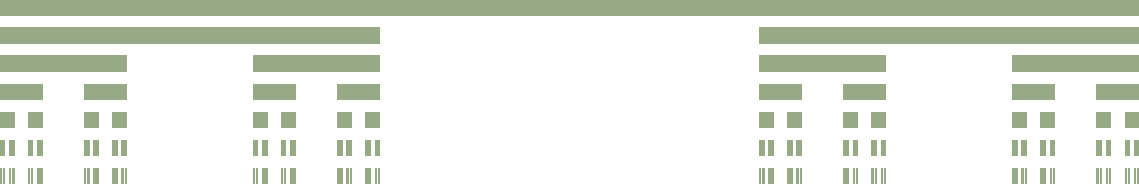
\includegraphics[width=16cm]{./attachment/cantor_set.pdf}
	\caption{Cantor集构造过程的示意图, 图源Wikipedia}
\end{figure}

Cantor集的构造过程用开集描述就是: 在第$n$次操作去掉(为了好写, 下面的开区间是包含已经去掉的部分的)$$I_n^1 = \big( \frac{1}{3^n},\frac{2}{3^n} \big), \quad  \cdots ,\quad I_n^k = \big( \frac{3k-2}{3^n},\frac{3k-1}{3^n} \big),\quad  \cdots , \quad I_n^{3^{n-1}} = \big( \frac{3^n-2}{3^n},\frac{3^n-1}{3^n} \big). $$

在分析Cantor集的性质之前, 需要定义: 

\begin{definition}{零测集}
	称一个集合$E \subseteq \R$是\textit{零测集}(null set), 如果对任意$\varepsilon >0$都存在至多可数个开区间组成的开覆盖$\{ I_n \}_{n \geq 1}$使得$\sum_{n=0}^{\infty} |I_n|<\varepsilon$. 
\end{definition}
\begin{remark}
	零测集的概念在Riemann积分部分还要使用. 
\end{remark}

无处稠密集的定义如同字面: 称$E$在$X$中无处稠密, 若对任意$x \in X$都存在邻域$U(x)$与$E$无交. 

\begin{proposition}{Cantor集的性质}
	Cantor集: 
	
	1) 是有限闭集(从而是紧集, 列紧集);\qquad 2) 是无处稠密集;
	
	3) 没有孤立点(这样的闭集称作完备集);\qquad 4) 是不可数集;\qquad 5) 是零测集. 
\end{proposition}
\begin{proof}
	(2) 对任意$x \in [0,1]$, 显然存在足够大的$n,k$使得$x \in I_n^k$. 
	
	(3) 对任意$x \in \mathcal{C}$, 设$N$满足对任意$n>N$, $x \in C_N$. 特别地对每个$n$取$I_n$是包含$x$的闭区间, 再从$I_n$任取$x_n \neq x$, 那么$x_n \to x$. 
	
	(4) \underline{\textbf{证法一}}~~(直观但不够严谨) 利用三进制来描述Cantor集的构造就是: 第$n$次操作去掉开区间$$I_n^k =  (0.a_1\cdots a_{n-1}1, 0.a_1\cdots a_{n-1}2),$$其中$0.a_1\cdots a_{n-1}=\frac{k}{3^{n-1}}$, $k$遍历$1,\cdots ,3^{n-1}$. 这就是说, $\mathcal{C} = \{ x:x\textit{的三进制表示中只有$0$或$2$} \}$. 将$\mathcal{C}$中的数的$2$全部变成$1$, 即得$\mathcal{C}$与$[0,1]$等势. 
	
	\underline{\textbf{证法二}}~~假设$\mathcal{C}$可数, 记$\mathcal{C} = \{ x_1,\cdots ,x_n,\cdots \}$. 下面归纳构造开区间列$\{ I_n \}$: 取$I_1 \subseteq [0,1]$使得$x_1 \in I_1$. 取$I_{n+1}$满足$$\overline{I_{n+1}} \subseteq I_n,\qquad x_n \notin \overline{I_{n+1}},\qquad I_{n+1} \cap \mathcal{C} \neq \varnothing .$$
	其中$I_{n+1} \cap \mathcal{C} \neq \varnothing$是由(3)保证的. 定义$K_n = \overline{I_n} \cap \mathcal{C}$, 则有紧集套$K_1 \supseteq \cdots \supseteq K_n \supseteq \cdots$, 于是$\cap_{n \geq 1}K_n \neq \varnothing$. 但是这与$x_n \notin K_{n+1}$矛盾. 
	
	(5) 任何一个$C_n$都能够覆盖$\mathcal{C}$, 而$|C_n| = 2^n \cdot \frac{1}{3^n} = \big( \frac{2}{3} \big)^n \to 0$, 因此$\mathcal{C}$是零测集. 
\end{proof}
\begin{remark}
	使用无限小数做证明的缺点在于: 例如$1/3$的三进制表示可以为$0.022\cdots$, 也可以为$0.1$, 我们需要人为约定只应用第一种情况. 
\end{remark}
\begin{remark}
	后面我们会证明, 可数集一定是零测集, 于是Cantor集成为了反面不成立的例子. 
\end{remark}











\chapter{一元函数微分学}

\section{导数与微分}

\subsection{导数的概念与计算}

导数的概念高中已经学过, 这里只是快速回顾(和严格化): 

\begin{definition}{导数}
	设$f:E \to \R$, $f$在$x_0$附近有定义. 称$f$在$x_0$处\textit{可导}(derivable), 如果下列极限存在(且有限): 
	$$\lim_{\Delta x \to 0} \frac{f(x_0+\Delta x) - f(x_0)}{\Delta x}, $$
	并记$f$在$x_0$的\textit{导数}(derivative)为该极限值. 
\end{definition}
\begin{remark}
	若$f$在$x_0$处可导, 显然$f$在$x_0$处连续. (反之则不一定! 如$f(x)=|x|$在$x=0$处连续但不可导)
\end{remark}
\begin{remark}
	$f$在$x_0$处的导数有以下主流记号: $$f'(x_0),\quad \frac{\dif }{\dif x} f(x) \big|_{x=x_0},\quad \dot{f}(x_0). $$
	第一种比较常见; 第二种将导数和微分联系起来(但现在我们暂且将其看做算子), 并提示我们考虑$f$的逐点导数; 第三种在物理学中常见. 
\end{remark}
\begin{remark}
	若$f$在$E$上逐点可导, 则称$f':E \to \R ,x \to f'(x)$为其导(函)数. 若$f'$连续, 则称$f$($1$-阶)连续可导, 并记所有这样的函数组成集合$C^1(E)$. 
\end{remark}
\begin{remark}
	若$f'$仍然在$E$上可导, 我们可以求出$f$的二阶导数$f''$, 以此类推. 一般地, 记$f$的$n$阶导数为$f^{(n)}$或$\frac{\dif ^n f}{\dif x^n}$. 另外, 若$f^{(n)}$是连续的, 则称$f$是$n$-阶连续可导的, 记所有这样的函数组成集合$C^{n}(E)$. 
\end{remark}
\begin{remark}
	当然可以定义所谓单侧导数, 并注意到$f$在$x_0$处可导当且仅当左导数$f'_-(x_0)$等于右导数$f'_+(x_0)$. 
\end{remark}
\begin{remark}
	当然可以定义导数为无穷的情况, 但我们不认为这是可导. 
\end{remark}

注意到, 若$f$在$x_0$处可导, 则$f$在局部可以写成以下形式: $$f(x_0+\Delta x) = f(x_0) + f'(x_0) \Delta x + o(\Delta x),\quad \Delta x \to 0. $$
该式子实际上就引入了微分的概念(见下一小节). 

\begin{proposition}{导数的四则运算}
	设$f,g$在$x$处可导. 则: 
	\begin{itemize}
		\item $f \pm g$在$x$处可导, 且$(f \pm g)'(x) = f'(x) \pm g'(x)$. 
		\item $f \cdot g$在$x$处可导, 且$(f\cdot g)'(x)=f'(x)g(x)+f(x)g'(x)$.
		\item (若$g \not\equiv 0$)$\frac{f}{g}$在$x$处可导, 且$\displaystyle \big( \frac{f}{g} \big)'(x) = \frac{f'(x)g(x)-f(x)g'(x)}{(g(x))^2}$. 
	\end{itemize}
\end{proposition}
\begin{proof}
	读者应当在中学就完成了这些公式的证明. 
\end{proof}

\begin{proposition}{Leibniz公式}
	设$f,g$在$x$处存在$n$次导数, 则
	\begin{center}
		$\displaystyle (f \cdot g)^{(n)}(x) = \sum_{k=0}^{n} \binom{n}{k} f^{(k)}(x)g^{(n-k)}(x)$. 
	\end{center}
\end{proposition}
\begin{proof}
	用归纳法和基本的组合数知识可以证明. 
\end{proof}

\begin{theorem}{复合函数的导数(链式法则)}
	设$f$在$x_0$处可导, $g$在$f(x_0)$处可导, 则$g\circ f$在$x_0$处可导, 且
	\begin{center}
		$(g\circ f)'(x_0)=g'(f(x_0))f'(x_0)$. 
	\end{center}
\end{theorem}
\begin{remark}
	复合函数的$n$次导数也有公式, 就是所谓Faà di Bruno公式. 
\end{remark}
\begin{proof}
	由之前的公式, 可知$$f(x_0+h)=f(x_0)+f'(x_0)h+o(h),\qquad g(f(x_0)+\ell )=g(f(x_0))+g'(f(x_0))\ell +o(\ell ).$$
	于是
	\begin{align*}
		\frac{g(f(x_0+h))-g(f(x_0))}{h} &= \frac{g( f(x_0)+f'(x_0)h+o(h) ) - g(f(x_0))}{h} \\
		&= \frac{g'(f(x_0)) \cdot (f'(x_0)h+o(h)) + o(f'(x_0)h+o(h))}{h} \\
		&= g'(f(x_0)) \cdot \left(f'(x_0) + \frac{o(h)}{h} \right) + o\left( f'(x_0)+\frac{o(h)}{h} \right) \\
		&\to g'(f(x_0))f'(x_0),\quad h \to 0. 
	\end{align*}
	其中, 我们令$\ell = f'(x_0)h+o(h)$, 显然当$h\to 0$时$\ell \to 0$, 因此上方的代换是合理的. 
\end{proof}
\begin{remark}
	如果直接用导数的定义式计算, 可能会出现$f(x)-f(x_0)$出现在分母上且为$0$的情况. 
\end{remark}

链式法则这个名字源自于上方定理的Leibniz记号表示: $$\frac{\dif z}{\dif x} = \frac{\dif z}{\dif y} \cdot \frac{\dif y}{\dif x}. $$
其中$z=g \circ f, y=f$. 我们不应将这个式子视作是简单的消元. 

\begin{theorem}{反函数的导数} \label{thm:fjhjuudedcuu}
	设$f$在区间$I$上连续且可逆. 若$f$在$x_0$处可导且$f'(x_0) \neq 0$, 则$f^{-1}$在$y_0=f(x_0)$处可导, 且有$$(f^{-1})'(y_0)=\frac{1}{f'(f^{-1}(y_0))}. $$
\end{theorem}
\begin{remark}
	一个小提醒: 若函数在一点连续, 其反函数不一定在该点对应的函数值处连续. (构造反例并不简单)
\end{remark}
\begin{proof}
	由$f$连续且可逆, 不妨设$f$单调递增, 那么$f^{-1}$单调递增且连续. 设$f(x_0)=y_0$, 则对于$y_0$的某个邻域$N_{\varepsilon}(y_0)$, 若$f^{-1}N_{\varepsilon}(y_0) = (x_0-\delta _1,x_0+\delta _2)$, 则当$y$从左至右遍历$N_{\varepsilon}(y_0)$时, $f^{-1}(y)$恰好从左至右遍历$(x_0-\delta _1,x_0+\delta _2)$. 特别地, $y \to y_0$等价于$x \to x_0$. 于是$$\lim_{y \to y_0} \frac{f^{-1}(y)-f^{-1}(y_0)}{y-y_0} = \lim_{y \to y_0} \left( \frac{f(x)-f(x_0)}{x-x_0} \right)^{-1} = \left( \lim_{x \to x_0}  \frac{f(x)-f(x_0)}{x-x_0} \right)^{-1} = \frac{1}{f'(x_0)}. $$
	其中, 第二个等号用到了上方“方向一致的一一对应”的想法. 
\end{proof}

现在来计算一些函数的导数: 

\begin{example}
	求$f(x)=e^x$的导数. 
\end{example}
\begin{solution}
	前面证明过, $\lim_{x \to 0} \frac{e^x-1}{x} = 1$. 于是$$\lim_{\Delta x \to 0} \frac{e^{x_0+\Delta x} - e^{x_0}}{\Delta x} = e^{x_0} \lim_{\Delta x \to 0} \frac{e^{\Delta x}-1}{\Delta x} = e^{x_0}. $$
	即$f'(x)=e^x$. 
\end{solution}

\begin{example}
	求$f(x) = \ln x$的导数. 
\end{example}
\begin{solution}
	一方面, 由反函数导数定理可以直接得到$f'(x)=\frac{1}{x}$. 另一方面, 亦可以注意到$$\lim_{\Delta x \to 0} \frac{\ln (x_0+\Delta x) - \ln x_0}{\Delta x} = \lim_{\Delta x \to 0} \frac{\ln \left( (1+\frac{\Delta x}{x_0})^{\frac{x_0}{\Delta x}} \right)}{x_0} = \frac{\ln \left(\lim_{\Delta x \to 0}  (1+\frac{\Delta x}{x_0})^{\frac{x_0}{\Delta x}} \right)}{x_0} = \frac{1}{x_0}. $$
\end{solution}

\begin{example}
	求$f(x)= \sin x$的导数. 
\end{example}
\begin{solution}
	注意到$$\lim_{\Delta x \to 0} \frac{\sin (x_0+\Delta x) - \sin x_0}{\Delta x} = \lim_{\Delta x \to 0} \frac{2\cos (x_0+\frac{\Delta x}{2}) \sin \frac{\Delta x}{2}}{\Delta x} = \cos \left( \lim_{\Delta x \to 0}\left( x_0+\frac{\Delta x}{2} \right) \right) \cdot \lim_{\Delta x \to 0} \frac{\sin \frac{\Delta x}{2}}{\frac{\Delta x}{2}} = \cos x_0. $$
\end{solution}

\begin{example}
	定义\textit{双曲正弦函数}$\sinh x:= \frac{1}{2}(e^x-e^{-x})$, \textit{双曲余弦函数}$\cosh x := \frac{1}{2}(e^x+e^{-x})$. 不难验证$\sinh$是单增的奇函数, $\cosh$是恒正的偶函数. 另外双曲函数具有和三角函数类似的性质, 如$\cosh ^2x - \sinh ^2x = 1$. 
	
	计算$\sinh x$和$\arsinh y$的导数. 
\end{example}
\begin{solution}
	易见$(\sinh x)'=\frac{1}{2}(e^x+e^{-x})=\cosh x$. 另外, 计算可得$\arsinh y = \ln (y+\sqrt{1+y^2})$. 于是$$(\arsinh y)' = \frac{1}{y+\sqrt{1+y^2}} \cdot \left( 1+\frac{y}{\sqrt{1+y^2}} \right) = \frac{1}{\sqrt{1+y^2}}. $$
\end{solution}
\begin{remark}
	我们注意到利用$e^x$的表示形式很容易求出$\arsinh$的导数. 类似地, $\sin x = \frac{1}{2}(e^{\ic x} - e^{-\ic x})$. 这启发我们研究复数域$\C$(或者说$\R ^2$)上函数的导数. 
\end{remark}

现在给出一张常见函数的导数表: 

\begin{figure}[H]
	\centering
	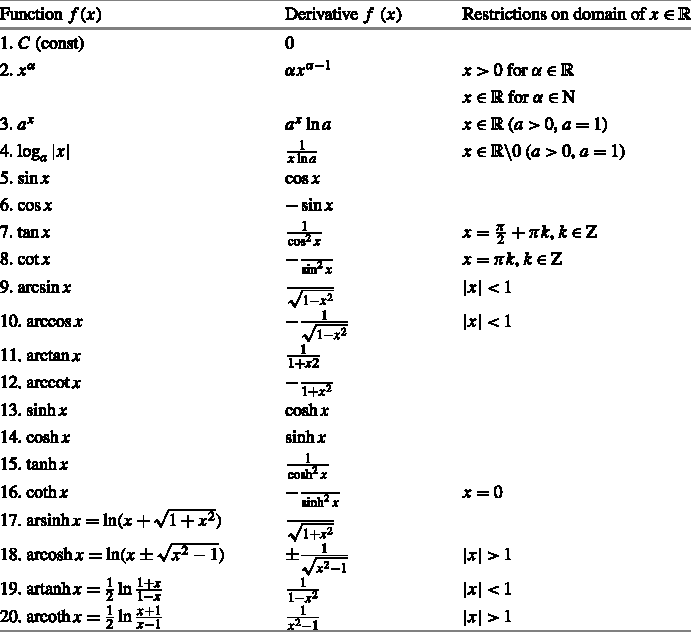
\includegraphics[width=13.5cm]{attachment/常见函数的导数.pdf}
	\caption{常见函数的导数表, 图源Zorich Table 5.1}
\end{figure}

\subsection{微分的概念}

上一节我们提到了这样一个公式: $$\Delta f(x) = f(x_0+\Delta x) - f(x_0) = f'(x_0) \Delta x + o(\Delta x),\quad \Delta x \to 0. $$
也就是说, 我们找到了一个线性函数$f'(x_0)\Delta x$来近似$\Delta f(x)$, 并且误差是关于$\Delta x$的无穷小量. 这样就产生了一个问题: 系数是$f'(x_0)$的线性函数的近似程度是否是最佳的? 我们会在后面给出解答. 

\begin{definition}{微分}
	设$f$在$x_0$附近有定义, 若存在$\lambda \in \R$使得$$f(x_0+\Delta x)-f(x_0) = \lambda \Delta x+o(\Delta x),\quad \Delta x \to 0,$$
	则称$f$在$x_0$处\textit{可微}(differentiable), 线性函数$\lambda \Delta x$为$f$在$x_0$处的\textit{微分}(differential), 记作$\dif f(x_0)$. 
\end{definition}

由上方的公式可知, 若$f$在$x_0$处可导, 则一定可微, 且系数$\lambda = f'(x_0)$. 反过来, 若$f$在$x_0$处可微, 在定义式的两边除以$\Delta x$并令$\Delta x \to 0$, 即得$f'(x_0) = \lambda$, 特别地$f$在$x_0$处可导. 

我们知道对于线性函数$f(x)=x$, 其微分恰好为$\Delta x$, 因此可以用记号$\dif x$代替$\Delta x$. 于是就有

\begin{proposition}{一元函数导数与微分的关系}
	一元函数$f$在$x_0$处可微当且仅当$f$在$x_0$处可导, 且
	\begin{center}
		$\dif f(x_0) = f'(x_0) \dif x. $
	\end{center}
\end{proposition}

该命题说明了记号$f'(x_0) = \frac{\dif f}{\dif x} \big|_{x=x_0}$的实际意义. 另外, 结合链式法则, 我们可以得到$$\dif g(f(x)) = g'(f(x)) f'(x)\dif x = g'(f(x)) \dif f(x). $$
该公式会在不定积分一节经常使用. 

从几何的观点来看, 在寻找一条曲线的切线时, 我们希望将切线定义为割线的极限位置, 而微分看起来就是这条切线(的某条平行线). 用形式化的语言写出来就是下方的定理: 

\begin{theorem}{微分最佳逼近定理}
	设$f$在$x_0$处可微, $\ell$是$f$在$x_0$处的\textit{切线}(tangent line), 定义为$\ell (x) = f(x_0)+f'(x_0)(x-x_0). $ \\
	则对于任意不等于$\ell (x)$的一次多项式$L(x)$都存在$\delta >0$, 使得对任意$x \in \mathring{N}_{\delta}(x_0)$都有
		$$|f(x)-\ell (x)| < |f(x)-L(x)|.$$
\end{theorem}
\begin{proof}
	当$L(x_0) \neq f(x_0)$时, 注意到$$\lim_{x \to x_0} |f(x) - L(x)| = |f(x_0)-L(x_0)|>0=\lim_{x\to x_0}|f(x)-\ell (x)|.$$
	由极限保序性知原命题成立. 
	
	当$L(x_0) = f(x_0)$时, 记$L(x)=f(x_0)+k(x-x_0)$, 那么$$\frac{|f(x)-\ell (x)|}{|f(x)-L(x)|} = \frac{o(x-x_0)}{(f'(x_0)-k)(x-x_0)+o(x-x_0)} \to 0,\quad x \to x_0. $$
	立得原命题成立. 
\end{proof}

\begin{figure}[H]
	\centering
	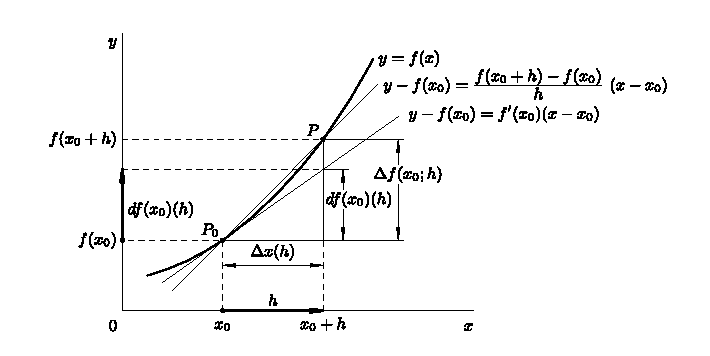
\includegraphics[width=12cm]{./attachment/differential_of_a_function.pdf}
	\caption{函数的割线, 切线, 微分等概念的示意图, 图源Zorich Fig. 5.3}
\end{figure}

利用微分形式, 可以较为方便地做计算. 

\begin{example}
	有些时候我们会遇到一些不便于写成显式表达式的函数, 例如椭圆方程$\displaystyle \frac{x^2}{a^2}+\frac{y^2}{b^2}=1$. 这时一般有两种表达方式: 隐式方程(即上式)或参数方程$\begin{cases}
	x=a\cos \theta \\ y=b\sin \theta
\end{cases},\theta \in [0,2\pi )$. 那么可以按如下方式求导: 
$$1)\quad 0 = \frac{\dif}{\dif x} 1 = \frac{\dif}{\dif x} \frac{x^2}{a^2} + \frac{\dif}{\dif x} \frac{y^2}{b^2} = \frac{2x}{a^2} + \frac{1}{b^2} \cdot \frac{\dif y^2}{\dif y} \cdot \frac{\dif y}{\dif x} = \frac{2x}{a^2} + \frac{2y}{b^2} \cdot y'\qquad \Leftrightarrow \qquad y' = -\frac{b^2x}{a^2y}. $$
并且注意到这样求出来的导数并不需要将椭圆拆成两半(以此保证函数良定义), 只需要将对应的横纵坐标代入. 
$$2)\quad y' = \frac{\dif y}{\dif x} = \frac{\dif y}{\dif \theta} \cdot \left( \frac{\dif x}{\dif \theta} \right)^{-1} = -\frac{b}{a} \cdot \frac{1}{\tan \theta} = -\frac{b^2x}{a^2y}. $$
当然最后一步代换不是必要的(因为一般写参数方程就是为了统一自变量). 
\end{example}

\begin{example}
	设$f$在$x$处存在$2$阶导数. 那么
	\begin{center}
		$\dif ^2 f(x) := \dif (\dif (f(x))) = \dif (f'(x) \dif x) = (f'(x) \dif x)' \dif x = f''(x) (\dif x)^2 =: f''(x) \dif x^2. $
	\end{center}
	注意在第4个等号处, $\dif x=\Delta x$是关于$x$的常数, 因此可以直接提出来. 这说明了高阶导数记号的意义. 
\end{example}



\newpage
\section{微分学的中值定理}

\subsection{函数的导数与其局部性质}

为了得到后面的重要定理, 我们先来研究导数所引出的函数局部性质: 

\begin{lemma}{}
	设开区间$I \subseteq \R$, $f:I \to \R$在$x_0$处可导且$f'(x_0)>0$. 那么存在$x_0$的邻域$N_{\delta}(x_0)$使得$f(x)-f(x_0)$在$x_0+\delta>x>x_0$时恒正, 在$x_0-\delta<x<x_0$时恒负. 
\end{lemma}
\begin{proof}
	易知存在$\delta$使得对任意$x\in N_{\delta}(x_0)$, $$\left| \frac{f(x)-f(x_0)}{x-x_0}-f'(x_0) \right| < \frac{1}{2}f'(x_0) \quad \Rightarrow \quad \frac{f(x)-f(x_0)}{x-x_0} > \frac{1}{2}f'(x_0) >0.$$
	即$f(x)-f(x_0)$与$x-x_0$同号. 
\end{proof}

\begin{proposition}{}
	设开区间$I\subseteq \R$, $f:I \to \R$在$I$上可导且对任意$x \in I$, $f'(x)>0$, 则$f$在$I$上严格单调递增. 
\end{proposition}
\begin{remark}
	该命题的不足之处在于: 若$f'(x) \geq 0$, 我们并不能说明$f$是单调不减函数. 这一结论将利用中值定理证明. 
\end{remark}

在下方的定理中, 局部极大(极小)值的定义为: 若存在邻域$N_{\delta}(x_0)$使得$f(x_0)$是$f$在$N_{\delta}(x_0)$上的最大(小)值, 则称$f(x_0)$为局部极大(极小)值. 

\begin{lemma}{Fermat引理}
	设$f:E \to \R$在$x_0$处可导, 则$f$在$x_0$处取得局部极值的必要条件是$f'(x_0)=0$. 
\end{lemma}
\begin{proof}
	设若不然, 不妨$f'(x_0)>0$, 则在$x_0$的某个邻域中对$x>x_0$总有$f(x)>f(x_0)$, 故$f(x_0)$不是局部极大值, 同理也不是局部极小值. 
\end{proof}

一般地, 称使得$f'(x_0)=0$的点$x_0$为$f$的\textit{驻点}(stationary point). 后面会看到, 通过计算$f''(x_0)$可以判断一个驻点$x_0$是否是极值点以及$f(x_0)$是极大值还是极小值. 

\subsection{Lagrange中值定理}

回顾\textit{无穷小增量公式}: $$f(x+h)-f(x)=f'(x)h+o(h),\quad h \to 0.$$
我们可以发现, 当$h \to 0$时, 上述公式实际上在用某点处的导数和定义域长度$h$的乘积描述$f$在初末位置取值的差. 那么能否将$h \to 0$的情况推广? 即让$f:[a,b] \to \R$, 是否存在$\xi \in [a,b]$使得$f(b)-f(a)=f'(\xi) (b-a)$? 我们从一个必要的情况出发考虑, 并将其作为引理. 

\begin{theorem}{Rolle中值定理}
	设$f$在$[a,b]$上连续, 在$(a,b)$上可导. 若$f(a)=f(b)$, 则存在$\xi \in (a,b)$使得$f'(\xi )=0$. 
\end{theorem}
\begin{proof}
	由$f$在$[a,b]$上连续可知$f$可取得最大值$M$和最小值$m$. 若$M=m$则$f'(x) \equiv 0$; 若$M>m$, 不妨$M>f(a)=f(b)$, 则存在$\xi$使得$f(\xi)=M$即$f'(\xi) = 0$. 
\end{proof}

\begin{theorem}{Lagrange中值定理}
	设$f$在$[a,b]$上连续, 在$(a,b)$上可导. 则存在$\xi \in (a,b)$使得$f'(\xi) = \dfrac{f(b)-f(a)}{b-a}$. 
\end{theorem}
\begin{remark}
	等价且好用的说法是: 存在$\theta \in (0,1)$使得$f'(a+\theta h)=\frac{f(a+h)-f(a)}{h}$, 其中$h=b-a$. 
\end{remark}
\begin{proof}
	构造函数$F(x)=f(x)-\frac{f(b)-f(a)}{b-a}(x-a)$, 则$F(a)=F(b)=f(a)$, 所以存在$\xi \in (a,b)$使得$F'(\xi)=0$, 也就是$f'(\xi) = \frac{f(b)-f(a)}{b-a}$. 
\end{proof}

\begin{figure}[H]
	\centering
	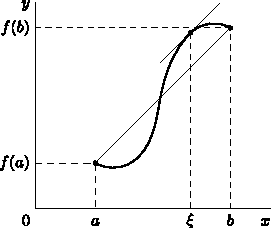
\includegraphics[width=6cm]{./attachment/Lagrange中值定理.pdf}
	\caption{Lagrange中值定理示意图, 图源Zorich Fig. 5.9}
\end{figure}

需要注意的是, 上面两个定理无法推广到向量值函数. 例如, 令$\bb{r}:[0,2\pi] \to \R ^2,t \mapsto (\cos t,\sin t)$, 可知$\bb{r}(0)=\bb{r}(2\pi)$但是$\bb{r}'(t) = (-\sin t,\cos t) \neq \bb{0}, t \in [0,2\pi]$. 

不过, 这个例子的物理意义是某物体以角速度$\omega =1$沿单位圆作匀速圆周运动. 而根据物理知识, 我们知道位移大小不会超过速度的最大值与时间的乘积, 即$|\bb{r}(b)-\bb{r}(a)| \leq |b-a| \cdot \sup_{t\in [a,b]} |\bb{r}'(t)|$. 这个增量估计公式将在多元微积分学中出现. 

\begin{corollary}{}
	设$f$在$[a,b]$上连续, 在$(a,b)$上可导. 则$f$在$[a,b]$上为常值函数当且仅当在$(a,b)$上$f'(x)=0$. 
\end{corollary}
\begin{remark}
	在定义不定积分时需要用到该命题. 
\end{remark}
\begin{proof}
	必要性显然. 充分性: 对任意$a \leq x_1 < x_2 \leq b$, 可知存在$\xi \in (x_1,x_2)$使得$f'(\xi) = \frac{f(x_2)-f(x_1)}{x_2-x_1} \equiv 0$, 因此$f$在$[a,b]$上为常值函数. 
\end{proof}

\begin{corollary}{}
	设$f$在$[a,b]$上连续, 在$(a,b)$上可导. 则$f$单调不减当且仅当$f'(x) \geq 0$. 
\end{corollary}
\begin{proof}
	必要性显然. 充分性: 若不然, 则存在$a \leq x_1 < x_2 \leq b$使得$f(x_1) > f(x_2)$, 由Lagrange中值定理可知存在$\xi \in (x_1,x_2)$使得$f'(\xi) = \frac{f(x_2)-f(x_1)}{x_2-x_1} <0$, 矛盾. 
\end{proof}

\subsection{导函数的性质}

为了得到导函数的中值定理, 我们当然希望(连续)函数的导函数一定连续, 但下方的例子指出这不一定成立. 

\begin{example}
	设$f(x) = \begin{cases}
		x^2\sin \frac{1}{x} & x \neq 0 \\ 0 & x=0
	\end{cases}$, 证明$f'(x)$在$0$处不连续. 
\end{example}
\begin{proof}
	当$x \neq 0$时, $f'(x) = 2x\sin \frac{1}{x}-\cos \frac{1}{x}$. 当$x = 0$时, $f'(x) = \lim_{h \to 0} \frac{h^2\sin \frac{1}{h}}{h} = 0$. 但是只需取$x_n = \frac{1}{2n\pi}, y_n = \frac{1}{(2n+1)\pi}$即有$x_n \to 0,y_n \to 0$且$f'(x_n) \to -1, f'(y_n) \to 1$, 这就是说$f'(x), x \neq 0$在$0$处不存在极限. 
\end{proof}

继续研究上方的例子. 笔者最初的证明思路是证明$f'(x), x \neq 0$在$0$处即使存在极限也不是$0$(这当然是对的, 例如只取上方的$x_n$就能说明). 不过, 更一般地我们会思考, 导函数如果不连续, 其间断点是否能是第一类间断点? 

答案是否定的. 

\begin{lemma}{}
	设$f$在$[a,b]$上连续, 在$(a,b)$上可导. 若$f'$在$a$处的右极限存在(且有限), 则$f$在$a$处的右导数存在且$f'_+(a)=f'(a+)$. 
\end{lemma}
\begin{proof}
	对任意$0<h<b-a$, 由Lagrange中值定理可知存在$\theta \in (0,1)$使得$f'(a+\theta h) = \frac{f(a+h)-f(a)}{h}$. 令$h \to 0^+$即可. 
\end{proof}

\begin{proposition}{}
	设$f$在$(a,b)$上可导. 则$f'$不存在第一类间断点. 
\end{proposition}
\begin{proof}
	假设存在$a<x_0 <b$使得$f'(x_0-)$和$f'(x_0+)$均存在. 那么$f'_-(x_0)$和$f'_+(x_0)$均存在, 但是由$f$在$x_0$可导, $f'(x_0-)=f'_-(x_0)=f'_+(x_0)=f'(x_0+)$, 故$f'$在$x_0$一定连续. 
\end{proof}

现在我们来研究导函数的中值定理: 

\begin{theorem}{Darboux}
	设$f$在$[a,b]$上可导, $f'(a)<f'(b)$, 则对任意$c \in (f'(a),f'(b))$存在$\xi \in (a,b)$使得$f'(\xi) = c$. 
\end{theorem}
\begin{proof}
	令$F(x)=f(x)-cx$, 则$F'(a)<0<F'(b)$, 因此$F$不是单调函数, 从而存在$a < x_1 < x_2 < b$使得$F(x_1)=F(x_2)$, 由Rolle中值定理可得存在$\xi \in (x_1,x_2)$使得$F'(\xi)=f'(\xi)-c=0$. 
\end{proof}



\subsection{Cauchy中值定理}

前文提到, Lagrange中值定理不好推广到向量值函数, 但是我们可以考虑换一种形式. 设曲线的参数方程$\begin{cases}
	x=x(t) \\ y=y(t)
\end{cases},a \leq t \leq b$. 若$x,y$在$[a,b]$上连续, 在$(a,b)$上可导, 在曲线上是否存在平行于过两端点$(x(a),y(a)),(x(b),y(b))$的直线? 利用前文提到的参数式求导方法, 我们实际在找$\xi \in (a,b)$使得$$\frac{y'(\xi)}{x'(\xi)} = \frac{y(b)-y(a)}{x(b)-x(a)}. $$

\begin{theorem}{Cauchy中值定理}
	设$f,g$在$[a,b]$上连续, 在$(a,b)$上可导. 若对任意$x \in (a,b)$, $g'(x) \neq 0$, 则存在$\xi \in (a,b)$使得$$\frac{f'(\xi)}{g'(\xi)} = \frac{f(b)-f(a)}{g(b)-g(a)}. $$
\end{theorem}
\begin{remark}
	虽然Cauchy中值定理的几何意义很好, 它一般的用途(刻意考察该定理的题目以外)只是证明l’Hôpital法则. 
\end{remark}
\begin{remark}
	这个式子是定义良好的: 由Lagrange中值定理, 存在$c \in (a,b)$使得$g(b)-g(a) = g'(c)(b-a) \neq 0$, 因此$g(b) \neq g(a)$. 
\end{remark}
\begin{proof}
	\underline{\textbf{证法一}}~~令$$h(x)=\frac{f(b)-f(a)}{g(b)-g(a)}(g(x)-g(a))-(f(x)-f(a)), $$
	由于$h(a)=h(b)=0$, 由Rolle中值定理可知存在$\xi \in (a,b)$使得$$0=h'(\xi)=\frac{f(b)-f(a)}{g(b)-g(a)} g'(\xi) - f'(\xi) \quad \Leftrightarrow \quad \frac{f'(\xi)}{g'(\xi)} = \frac{f(b)-f(a)}{g(b)-g(a)}. $$
	
	\underline{\textbf{证法二}}~~由于$g'(x) \neq 0$, $g'(x)$应当不变号(否则由Darboux定理, 存在$c$使得$g'(c)=0$), 即$g$是$[a,b] \to [g(a),g(b)]$的连续双射. 考虑$f \circ g^{-1}:[g(a),g(b)] \to \R$, 对该函数应用Lagrange中值定理可知, 存在$\xi \in (g(a),g(b))$使得$$\frac{fg^{-1}(g(a))-fg^{-1}(g(b))}{g(a)-g(b)} = (fg^{-1})'(\xi) \quad \Leftrightarrow \quad \frac{f(b)-f(a)}{g(b)-g(a)} = \frac{f'(g^{-1}(\xi))}{g'(g^{-1}(\xi))}.$$
	其中$g^{-1}(\xi) \in (a,b)$, 为命题所求. 
\end{proof}

\subsection{中值定理的应用}

这一小节我们来看几个用到了中值定理的命题. 

\circled{A}~~反函数定理(逆映射定理)是多元微分学中的重要内容, 但在$\R$上我们能以非常轻松的方式证明. 

\begin{theorem}{反函数定理($C^1$版本)}
	设开区间$I \subseteq \R$, $f \in C^1(I)$, 且$f'(x_0) \neq 0$. 则$f$在$x_0$的一个邻域上是$C^1$-同胚, 即$$f|_{N_{\delta}(x_0)}:N_{\delta}(x_0) \to f(N_{\delta}(x_0)) = (f(x_0)-\varepsilon _1,f(x_0)+\varepsilon _1)$$
	是双射且其逆$f|_{N_{\delta}(x_0)}^{-1} \in C^1(I)$. 
\end{theorem}
\begin{proof}
	不妨$f'(x_0)>0$, 由$f'$连续可知存在$\delta$使得$f'$在$N_{\delta}(x_0)$上的取值恒正, 即$f$在$N_{\delta}(x_0)$上严格递增. 由定理\ref{thm:fjhjuudedcuu}可知$f$在$N_{\delta}(x_0)$可逆且其逆$f^{-1}$可微. 另外由$(f^{-1})'(y)=\frac{1}{f'(f^{-1}(y))}$可知$f^{-1}$是连续函数的复合, 即$f^{-1}$连续. 
\end{proof}

\begin{corollary}{反函数定理($C^{\infty}$版本)}
	承上述定理要求, 但是令$f \in C^{\infty}(I)$即$f$是光滑的, 则$f^{-1}$也是光滑的. 
\end{corollary}
\begin{proof}
	利用Faà di Bruno公式和$(f^{-1})'(y)=\frac{1}{f'(f^{-1}(y))}$即可. (但是计算很复杂)
\end{proof}

\circled{B}~~处处连续但处处不可导的函数: 此类函数有很多不同的构造, 这里只介绍最初版本的Weierstrass函数. 

定义(先承认三角函数的性质)$$f(x)=\sum_{n=0}^{\infty} a^n\cos (b^n\pi x). $$
其中$0<a<1$, $b$是正的奇数, $ab>M$($M$是待定的较大的数). 容易证明$\sum_{n=1}^{\infty} \| a^n\cos (b^n\pi x) \|_{\infty} \leq \sum_{n=1}^{\infty}a^n$, 从而原级数(绝对)收敛, 那么$f$连续. 

\begin{figure}[H]
	\centering
	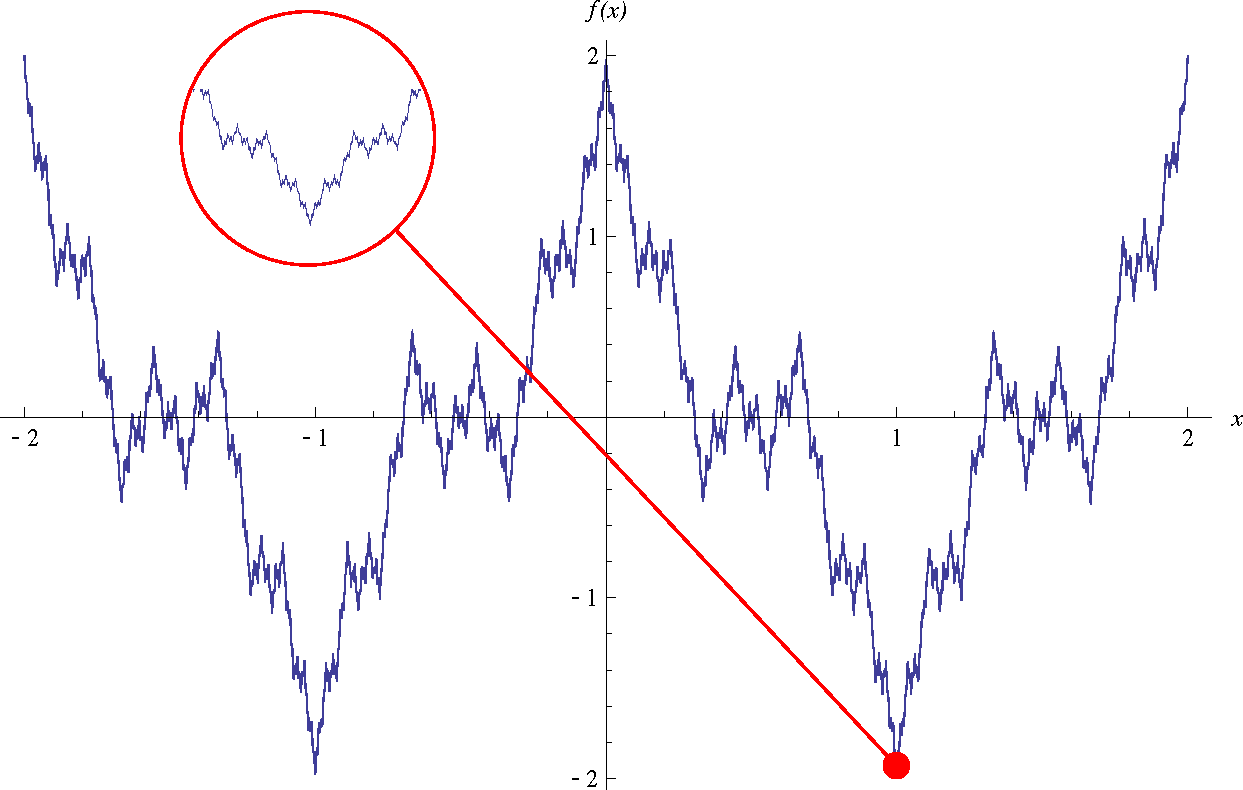
\includegraphics[width=10cm]{attachment/WeierstrassFunction.pdf}
	\caption{Weierstrass函数示意图, 图源Wikipedia}
\end{figure}

我们考虑证明$f$在任意一点不存在导数, 也就是让任意点处的斜率为无穷大. 固定$x$, 首先计算$$\frac{f(x+h)-f(x)}{h} = \sum_{n=0}^{\infty} a^n \frac{\cos (b^n\pi (x+h)) - \cos (b^n\pi x)}{h} = \sum_{n=0}^{m-1}(\cdots) + \sum_{n=m}^{\infty}(\cdots).$$
希望得到$$\left| \frac{f(x+h)-f(x)}{h} \right| \geq \left| \sum_{n=m}^{\infty}(\cdots) \right| - \left| \sum_{n=0}^{m-1}(\cdots) \right| > (\cdots ) \to +\infty .$$
因此需要估计(绝对值下)前一部分的上界和后一部分的下界. 先利用中值定理估计前一部分: 
\begin{align*}
	\left| \sum_{n=0}^{m-1}(\cdots) \right| &\leq \pi \sum_{n=0}^{m-1} (ab)^n \left| \frac{\cos (b^n\pi (x+h)) - \cos (b^n\pi x)}{b^n \pi h} \right| = \pi \sum_{n=0}^{m-1} (ab)^n |\sin (b^n\pi (x+\theta _n h))| \\ 
	&\leq \pi \sum_{n=0}^{m-1} (ab)^n = \pi \frac{(ab)^m-1}{ab-1}. 
\end{align*}
接下来, 令$b^mx=\alpha _m+\beta _m$, 其中$\alpha _m$是整数而$-1/2 \leq \beta _m < 1/2$. 于是$$\cos (b^n\pi x) = \cos (b^{n-m}\pi (\alpha _m + \beta _m)) = \cos (b^{n-m}\pi \alpha _m)\cos (b^{n-m}\pi \beta _m) = (-1)^{\alpha _m} \cos (b^{n-m}\pi \beta _m), $$
$$\cos (b^n\pi (x+h)) = \cos \left( b^{n-m}\pi(\alpha _m + \beta _m + b^mh) \right). $$
为了尽量化简, 可以令$b^mh=1-\beta _m$, 于是$\cos (b^n\pi (x+h)) = (-1)^{\alpha _m+1}$. 进而$$\left| \sum_{n=m}^{\infty}(\cdots) \right| = \frac{1}{|h|} \sum_{n=m}^{\infty} a^n(1+\cos (b^{n-m}\pi \beta _m)) > \frac{1}{h}a^m(1+\cos (\pi \beta _m)) > \frac{a^m}{h} > \frac{2}{3}(ab)^m. $$
其中关于$h$的放缩是因为$h = \frac{1-\beta _m}{b^m} \in [\frac{1}{2b^m},\frac{3}{2b^m}]$. 于是我们有$$\left| \frac{f(x+h)-f(x)}{h} \right| > (ab)^m \left( \frac{2}{3}-\frac{\pi}{ab-1} \right).$$
当$ab>1+\frac{3}{2}\pi$时右侧为正, 令$m \to \infty$(同时$h \to 0$)即得$f$在$x$处导数不存在. 


\circled{C}~~$\pi$的定义与三角函数的周期: 

在之前的补充习题中我们用幂级数定义了三角函数$$\cos z = \frac{e^{\ic z}+e^{-\ic z}}{2}= \sum_{k=0}^{\infty} \frac{(-1)^kx^{2k}}{(2k)!},\qquad \sin z = \frac{e^{\ic z} - e^{-\ic z}}{2\ic} = \sum_{k=0}^{\infty} \frac{(-1)^kx^{2k+1}}{(2k+1)!}, $$
并且顺带证明了三角函数的和角公式. 但是对三角函数至关重要的$\pi$值仍然没有定义. 现在用分析的方法定义$\pi$: 

首先, 通过求导容易证明$\sin x$在$(0,\delta)$上单调递增, $\cos x$在$(0,\delta)$上单调递减, 其中$\delta$是某个比较小的正数. 特别地, 由对称性, 易知$\cos x$在$x=0$处取得极大值$1$. 

接着我们要证明存在$\alpha >0$使得$\cos x$在$(0,\alpha)$上单调递减且$\cos \alpha =0$(同时$\sin \alpha =1$, 注意符号!), 另一方面存在$\beta >0$使得$\sin x$在$(\alpha ,\beta)$上单调递减且$\sin \beta =0$(同时$\cos \beta = -1$), 然后将$\beta$定义为$\pi$. 

\begin{proof}
	以第一条为例. 考虑使得$\cos x$在$(0,\alpha)$为正的最大的$\alpha$, 存在性由下方推理保证: 假设$\cos x$在$(0,+\infty)$均为正, 则$(\sin x)' = \cos x>0$, 即$\sin x$在$(0,+\infty)$单调递增, 从而存在极限$l>0$. 但是$(\cos x)' = -\sin x \searrow -l$, 这与$\cos x$有下界矛盾. 
	
	既然$\alpha \in \R$, 由$\cos x$的连续性可得$\cos \alpha=0$, 进而$\sin \alpha =1$(否则$\sin x$不会在$(0,\delta)$单调递增). 
\end{proof}

现在来考虑三角函数的周期. 令$S(x)=-\sin (x+\pi), C(x)=-\cos (x+\pi)$, 那么$S'(x) = -\cos (x+\pi) = C(x)$, $C'(x) = \sin (x+\pi) = -S(x)$, $S(0)=0, C(0)=1$. 令$f(x)=\begin{pmatrix}
	\sin x \\ \cos x
\end{pmatrix}$, $F(x) = \begin{pmatrix}
	S(x) \\ C(x)
\end{pmatrix}$. 我们不加证明地认为方程$$\begin{cases}
	f'(x)=Jf(x) \\ f(0)=I
\end{cases},\quad J=\begin{pmatrix}
		0 & 1 \\ -1 & 0
	\end{pmatrix}, I=\begin{pmatrix}
		0 \\ 1
	\end{pmatrix}$$存在唯一解(后面会证明), 于是$F(x) \equiv f(x)$. 这就是说$$-\sin (x+\pi) = \sin x,\qquad -\cos (x+\pi) = \cos x. $$
进而$\sin x$和$\cos x$的最小正周期都是$2\pi$. 

\subsection{l’Hôpital法则}

相信读者在高中已经熟悉了l’Hôpital法则的使用, 现在我们给出严格证明. 实际上, l’Hôpital法则包括$$x \to a^+, \quad x\to a^-, \quad x \to a, \quad x \to +\infty , \quad x \to - \infty , \quad x \to \infty$$
六种极限过程和$$f(x),g(x) \to 0,\qquad g(x) \to \infty$$
两种极限情况的各种组合情况. 我们只需要证明$x \to a^+$下两种极限情况, 立即可以推出剩下的情况. 

\begin{theorem}{$0/0$型l’Hôpital法则}
	设$f,g$在$(a,b)$上可导, 且对任意$x \in (a,b)$, $g'(x) \neq 0$. 若
	
	\begin{center}
		$\displaystyle \lim_{x \to a^+} f(x) = 0, \lim_{x \to a^+} g(x) = 0, $
	\end{center}
	
	\noindent
	且极限$\lim_{x \to a^+} \frac{f'(x)}{g'(x)}$存在, 则极限$\lim_{x \to a^+} \frac{f(x)}{g(x)}$也存在, 而且有
	
	\begin{center}
		$\displaystyle \lim_{x \to a^+} \frac{f(x)}{g(x)} = \lim_{x \to a^+} \frac{f'(x)}{g'(x)}. $
	\end{center}
\end{theorem}
\begin{proof}
	不妨令$f(a)=g(a)=0$, 从而$f,g$在$[a,b)$上连续. 对任意$x \in (a,b)$, 取$h \in (0,x-a)$, 由Cauchy中值定理可知存在$\theta \in (0,1)$使得$$\frac{f'(a+\theta h)}{g'(a+\theta h)} = \frac{f(x)-f(a)}{g(x)-g(a)} = \frac{f(x)}{g(x)}. $$
	在上式中令$x \to a^+$, 则$h \to 0^+$, 那么$$\lim_{x \to a^+} \frac{f'(x)}{g'(x)} = \lim_{h \to 0^+} \frac{f'(a+\theta h)}{g'(a+\theta h)} = \lim_{x \to a^+} \frac{f(x)}{g(x)}. $$
\end{proof}

\begin{theorem}{$\bigcdot/\infty$型l’Hôpital法则}
	设$f,g$在$(a,b)$上可导, 且对任意$x \in (a,b)$, $g'(x) \neq 0$. 若
	
	\begin{center}
		$\lim_{x \to a^+} g(x) = \infty, $
	\end{center}
	
	\noindent
	且极限$\lim_{x \to a^+} \frac{f'(x)}{g'(x)}$存在, 则极限$\lim_{x \to a^+} \frac{f(x)}{g(x)}$也存在, 而且有
	
	\begin{center}
		$\displaystyle \lim_{x \to a^+} \frac{f(x)}{g(x)} = \lim_{x \to a^+} \frac{f'(x)}{g'(x)}. $
	\end{center}
\end{theorem}
\begin{remark}
	尽管这里的适用范围是$\bigcdot/\infty$, 但是当$\bigcdot$有限时显然极限值为$0$, 因此$\infty/\infty$型才是常用的说法. 
\end{remark}
\begin{proof}
	只需证明$$\liminf_{x\to a^+} \frac{f'(x)}{g'(x)} \leq \liminf_{x\to a^+} \frac{f(x)}{g(x)} \leq \limsup_{x\to a^+} \frac{f(x)}{g(x)} \leq \limsup_{x\to a^+} \frac{f'(x)}{g'(x)}.$$
	
	以右侧为例. 记$s = \limsup_{x\to a^+} \frac{f'(x)}{g'(x)}$. 任取$s_1>s$, 存在$\delta$使得任意$x \in (a,a+\delta)$有$\frac{f'(x)}{g'(x)} <s_1$. 另外, 对任意$x \in (a,a+\delta)$, 由Cauchy中值定理可知, 存在$\xi \in (x,a+\delta)$使得$$\frac{f(x)-f(a+\delta)}{g(x)-g(a+\delta)} = \frac{f'(\xi)}{g'(\xi)} <s_1. $$
	这就是说$$\frac{f(x)}{g(x)} < s_1\left( 1-\frac{g(a+\delta)}{g(x)} \right) + \frac{f(a+\delta)}{g(x)} \to s_1,\quad x \to a^+.$$
	由$s_1$选取的任意性, $\lim_{x \to a^+} \frac{f(x)}{g(x)} \leq s$. 
\end{proof}
\begin{remark}
	该证明与之前Stolz定理的证明几乎相同. 
\end{remark}

\newpage
\section*{一些习题 ~~\small 对应原书5.2,5.3习题} \label{sec:ex6.1}

\subsection*{A: 中值定理的应用}

归纳地定义$f$在$x_0$处的$k$阶有限差: $$\Delta f(x_0;h_1) := f(x_0+h_1)-f(x_0), \qquad \Delta ^kf(x_0;h_1,\cdots ,h_k) := \Delta ^{k-1} (\Delta f(x;h_k)) (x_0;h_1,\cdots ,h_k). $$

\circled{A1}-1~~设$f \in C^{n-1}([a,b])$, 且在$(a,b)$上存在$n$阶导数. 设$x_0+h_1,\cdots ,x_0+h_1+\cdots +h_n$均包含于$[a,b]$, 那么存在包含这些点的最小闭区间内的点$\xi$使得$$\Delta ^n f(x_0;h_1,\cdots ,h_n) = f^{(n)}(\xi) h_1\cdots h_n. $$

\circled{A1}-2~~特别地, 记$\Delta ^nf(x_0;h^n) := \Delta ^nf(x_0;h,\cdots ,h)$. 若$f^{(n)}(x_0)$存在, 则$$f^{(n)}(x_0) = \lim_{h \to 0} \frac{\Delta ^n f(x_0;h^n)}{h^n}. $$

\circled{A1}-3~~函数$f(x)=\begin{cases}
	x^3\sin \frac{1}{x} & x\neq 0 \\ 0 & x = 0
\end{cases}$满足$\displaystyle \lim_{h\to 0} \frac{\Delta ^2 f(0;h^2)}{h^2}$存在但$f^{(2)}(0)$不存在. 
\vspace{1em}

设$f \in C^n((-1,1))$, $\sup_{x\in (-1,1)} |f(x)| \leq 1$. 记$m_k(I) = \inf_{x \in I} |f^{(k)}(x)|$. 
\vspace{1em}

\circled{A2}-1~~若将$I$依次分为区间$I_1,I_2,I_3$, 则$$m_k(I) \leq \frac{1}{|I_2|} (m_{k-1}(I_1) + m_{k-1}(I_3)). $$

\circled{A2}-2~~记$\lambda = |I|$, 则$$m_k(I) \leq \frac{2^{\frac{k(k+1)}{2}} k^k}{\lambda ^k}. $$

\circled{A2}-3~~存在只与$n$有关的$\alpha _n$, 使得若$|f'(0)| \geq \alpha _n$, 则$f^{(n)}(x)$在$(-1,1)$上有至少$n-1$个不同的零点. 








\newpage
\section{Taylor公式}

\subsection{带Peano余项的Taylor公式}

回顾无穷小增量公式$$f(x)=f(x_0)+f'(x_0)(x-x_0)+o(x-x_0),\quad x \to x_0.$$
现在我们希望将右侧的误差进一步缩小, 也即寻找常数$a_0,a_1,a_2$使得$$f(x) = a_0 + a_1(x-x_0) + a_2(x-x_0)^2 +o((x-x_0)^2),\quad x \to x_0. $$
由于$f$在$x_0$处连续, 可知$f(x_0)=a_0$. 进一步有$$\frac{f(x)-f(x_0)}{x-x_0} = a_1 + a_2(x-x_0) + o(x-x_0),\quad x \to x_0\quad \Leftrightarrow \quad f'(x_0)=a_1. $$
最后, 计算可得$$\frac{f(x)-f(x_0)-f'(x_0)(x-x_0)}{(x-x_0)^2} = a_2 + o(1), \quad x \to x_0 \quad \Leftrightarrow \quad a_2 = \frac{1}{2} \lim_{x \to x_0} \frac{f'(x)-f'(x_0)}{x-x_0} = \frac{1}{2}f''(x_0).$$
其中“$\Rightarrow$”方向使用了l’Hôpital法则, “$\Leftarrow$”方向是直接验证. 利用数学归纳法可以将这个想法推广: 

\begin{theorem}{带Peano余项的Taylor公式}
	设$f$在$x_0$附近有定义, 且在$x_0$处存在$n$阶导数. 则当$x \to x_0$时, $$f(x)=f(x_0)+\frac{1}{1!}f'(x_0)(x-x_0) + \cdots \frac{1}{n!}f^{(n)}(x_0)(x-x_0)^n + o((x-x_0)^n). $$
\end{theorem}
\begin{remark}
	最后的余项也可写作$O((x-x_0)^{n+1})$, 原因之前解释过. 
\end{remark}
\begin{remark}
	一般记$P_n(f,x_0;x)=f(x_0) + \cdots + \frac{1}{n!}f^{(n)}(x_0)(x-x_0)^n$为$f$在$x_0$处的$n$次Taylor多项式. 
\end{remark}
\begin{proof}
	归纳证明. 当$n=1$时显然. 假设当$n=k$时成立, 计算可得$$P'_{k+1}(f,x_0;x) = f'(x_0)+\frac{1}{1!}f''(x_0)(x-x_0) + \cdots + \frac{1}{k!}f^{(k+1)}(x_0)(x-x_0)^k = P_k(f',x_0;x).$$
	结合l’Hôpital法则, 我们有$$\lim_{x \to x_0} \frac{f(x)-P_{k+1}(f,x_0;x)}{(x-x_0)^{k+1}} = \frac{1}{k+1} \lim_{x \to x_0} \frac{f'(x)-P_k(f',x_0;x)}{(x-x_0)^k}=0.$$
	这就是说, $f(x)=P_{k+1}(f,x_0;x)+o((x-x_0)^{k+1})$. 
\end{proof}

为了让Taylor展开式尽可能简单, 我们习惯于令$x_0=0$, 得到的展开式称作\textit{Maclaurin展开式}. 现在来求一些函数的Maclaurin展开式(本质上就是求高阶导数): 

\begin{example}
	求$f(x)=\sin x$的Maclaurin展开式. 
\end{example}
\begin{solution}
	熟知$$\sin ^{(4k)} (x) = \sin x,\quad \sin ^{(4k+1)} (x) = \cos x,\quad \sin ^{(4k+2)} (x) = -\sin x,\quad \sin ^{(4k+3)} (x) = -\cos x. $$
	于是$f^{(2\ell )}(0)=0,f^{(2\ell +1)}(0)=(-1)^{\ell}$. 那么$$\sin x = x-\frac{1}{3!} x^3 + \cdots + \frac{(-1)^n}{(2n+1)!}x^{2n+1} + o(x^{2n+2}),\quad x\to 0.$$
\end{solution}

\begin{example}
	求$f(x)=\arctan x$的Maclaurin展开式. 
\end{example}
\begin{solution}
	由$f'(x)=(1+x^2)^{-1}$, 可知$(1+x^2)f'(x)=1$. 对两边求$k$阶导, 由Leibniz公式我们有$$(1+x^2)f^{(k+1)}(x) + 2kxf^{(k)}(x) + k(k-1)f^{(k-1)}(x)=0. $$
	令$x=0$, 即得递推关系$f^{(k+1)}(x)=-k(k-1)f^{k-1}(x)$. 于是$$\arctan x = x-\frac{1}{3}x^3+\cdots \frac{(-1)^n}{2n+1}x^{2n+1} + o(x^{2n+2}),\quad x\to 0. $$
\end{solution}

用类似的方法, 不难求得以下函数的Maclaurin展开式: 
\begin{itemize}
	\item $\displaystyle e^x = 1 + \frac{1}{1!}x + \cdots + \frac{1}{n!} x^n + o(x^{n}),\quad x\to 0.$
	\item $\displaystyle \ln (1+x) = x - \frac{1}{2}x^2 + \cdots + \frac{(-1)^{n-1}}{n} x^n + o(x^{n}),\quad x \to 0. $
	\item $\displaystyle (1+x)^{\alpha} = 1 + \frac{\alpha}{1!}x + \cdots \frac{\alpha \cdots (\alpha -n+1)}{n!} x^n + o(x^{n}),\quad x \to 0.$
	\item $\displaystyle \sin x = x-\frac{1}{3!} x^3 + \cdots + \frac{(-1)^n}{(2n+1)!}x^{2n+1} + o(x^{2n+2}),\quad x\to 0.$
	\item $\displaystyle \cos x = 1-\frac{1}{2!} x^2 + \cdots + \frac{(-1)^n}{(2n)!}x^{2n} + o(x^{2n+1}),\quad x\to 0.$
	\item $\displaystyle \arctan x = x-\frac{1}{3}x^3+\cdots \frac{(-1)^n}{2n+1}x^{2n+1} + o(x^{2n+2}),\quad x\to 0.$
	\item $\displaystyle \sinh x = x+\frac{1}{3!} x^3 + \cdots + \frac{1}{(2n+1)!}x^{2n+1} + o(x^{2n+2}),\quad x\to 0.$
	\item $\displaystyle \cosh x = 1+\frac{1}{2!} x^2 + \cdots + \frac{1}{(2n)!}x^{2n} + o(x^{2n+1}),\quad x\to 0.$
	\item $\displaystyle \artanh x = x+\frac{1}{3}x^3+\cdots \frac{1}{2n+1}x^{2n+1} + o(x^{2n+2}),\quad x\to 0. $
\end{itemize}

若要计算$\tan x$的Taylor展开, 我们需要Bernoulli数, 但这就是组合数学研究的对象了. 

另外, 我们观察到, 如$\sin x,\cos x,e^x$等函数的Maclaurin展开式和其幂级数形式非常类似(之后会介绍原因). 但是需要注意, 不能想当然地认为Maclaurin展开式直接可以推广为幂级数, 我们本质上还是在研究函数在一点处的性质. 反例如: 

\begin{example}
	设$f(x)=\begin{cases}
		e^{-\frac{1}{x^2}} & x \neq 0 \\ 0 & x = 0
	\end{cases}$. 则$f(x)=o(x^n)$对任意$n>0$成立. 
\end{example}
\begin{proof}
	计算可得$$f'(0)=\lim_{x \to 0} \frac{e^{-\frac{1}{x^2}}}{x} = 0,\quad f'(x)=\frac{2}{x^3}e^{-\frac{1}{x^2}},x \neq 0.$$
	通过猜测结合归纳法, 可以证明$$f^{(n)}(0) = 0,\quad f^{(n)}(x) = P_n(x)e^{-\frac{1}{x^2}},x \neq 0.$$
	其中$P_n(x)$满足如下递推关系: $P_0(x)=1,P_n(x)=\frac{2}{x^3}P_{n-1}(x)+P'_{n-1}(x)$. 
\end{proof}

这个例子同时能说明, 单纯提高Taylor多项式的次数不一定减小逼近误差. 

类似于微分最佳逼近定理, 我们有: 

\begin{theorem}{Taylor多项式最佳逼近定理}
	设$f$在$x_0$处存在$n$阶导数, 则对任意不等于$P_n(f,x_0;x)$且次数不超过$n$的多项式$P$, 均存在$\delta >0$使得对任意$x \in \mathring{N}_{\delta}(x_0)$都有$$|f(x)-P_n(f,x_0;x)| < |f(x)-P|.$$
\end{theorem}
\begin{proof}
	略. (提示: 对$P$应用Taylor展开)
\end{proof}

局部的Taylor公式通常用来求极限, 例如: 

\begin{example}
	求极限: $$\lim_{x\to 0} \frac{xe^x - \sin x -x^2}{\sin ^3 x}. $$
\end{example}
\begin{solution}
	首先将分母上的$\sin x$替换为$x$. 根据$\sin x = x - \frac{1}{3} x^3 + o(x^4)$和$e^x = 1+x+\frac{1}{2}x^2+o(x^3)$可知$$\textit{原式} = \lim_{x\to 0} \frac{1}{x^3}\left( x+x^2+\frac{1}{2}x^3 - x + \frac{1}{3}x^3 - x^2 +o(x^4) \right) = \frac{5}{6}. $$
\end{solution}


\subsection{对Taylor公式余项的定量研究}

之前介绍的带Peano余项的Taylor公式其实并没有真正给出余项$f(x)-P_n(f,x_0;x)$的值, 只是给出了余项的一个最终上界$(x-x_0)^{n+1}$. 类似于从无穷小增量公式到中值定理, 我们希望找到某个具体值$\xi$来描述余项. 

先从简单的情况写起: 设$f$具有待定的性质. $\varphi$在$[x_0,x]$上连续, 在$(x_0,x)$上可导且导数不为$0$. 首先由Cauchy中值定理, 存在$\xi \in (x_0,x)$使得
\begin{equation}
	\frac{f(x)-f(x_0)}{\varphi (x)-\varphi (x_0)} = \frac{f'(\xi)}{\varphi '(\xi)} \quad \Leftrightarrow \quad f(x) = P_0(f,x_0;x) + \frac{\varphi (x)-\varphi (x_0)}{\varphi '(\xi)} f'(\xi). \label{eq:taylor0}
\end{equation}

进一步, 我们希望右边仍然存在一个$P_1(f,x_0;x)$. 考虑令$F(t)=f(x)-(f(t)+f'(t)(x-t))$, 从而$F(x)-F(x_0)$恰好等于$f(x)-P_1(f,x_0;x)$. 现在, 对$F(t),\varphi (t)$应用Cauchy中值定理可知, 存在$\xi \in (x_0,x)$使得
\begin{equation}
	\frac{F(x)-F(x_0)}{\varphi (x)-\varphi (x_0)} = \frac{F'(\xi)}{\varphi '(\xi)} \quad \Leftrightarrow \quad f(x) = P_1(f,x_0;x) + \frac{\varphi (x) - \varphi (x_0)}{\varphi '(\xi)} f''(\xi)(x-\xi). \label{eq:taylor1}
\end{equation}

根据式\ref{eq:taylor0}和\ref{eq:taylor1}可以猜测下方定理的形式: 

\begin{theorem}{带定量余项的Taylor公式}
	设$f$在$(x_0,x)$上存在$n+1$阶导数, 在$[x_0,x]$上$n$-阶连续可导. 则对于在$[x_0,x]$上连续, 在$(x_0,x)$上可导且导数不为$0$的函数$\varphi$, 存在$\xi \in (x_0,x)$使得
	\begin{center}
		$\displaystyle f(x)=P_n(f,x_0;x) + \frac{\varphi (x) - \varphi (x_0)}{\varphi '(\xi) n!} f^{(n+1)}(\xi) (x-\xi )^n. $
	\end{center}
\end{theorem}
\begin{remark}
	将条件改为$(x,x_0)$和$[x,x_0]$也成立. 
\end{remark}
\begin{proof}
	构造函数$F(t)=f(x)-P_n(f,t;x)$. 显见$F$在$[x_0,x]$连续, 在$(x_0,x)$可导, 且$F'(t) = -\frac{f^{(n+1)}(t)}{n!}(x-t)^n$. 对$F(t),\varphi (t)$应用Cauchy中值定理, 则存在$\xi \in (x_0,x)$使得$$\frac{F(x)-F(x_0)}{\varphi (x)-\varphi (x_0)} = \frac{F'(\xi)}{\varphi '(\xi)}\quad \Leftrightarrow \quad \frac{P_n(f,x_0;x)}{\varphi (x)-\varphi (x_0)} = -\frac{f^{(n+1)}(\xi)}{\varphi '(\xi) n!}(x-\xi)^n. $$
\end{proof}

由这个定理, 马上可以得到两个常用推论: 

\begin{corollary}{带Lagrange余项的Taylor公式}
	设$f$在$(x_0,x)$上存在$n+1$阶导数, 在$[x_0,x]$上$n$-阶连续可导. 则存在$\xi \in (x_0,x)$使得
	\begin{center}
		$\displaystyle f(x)=P_n(f,x_0;x)+\frac{f^{(n+1)}(\xi)}{(n+1)!} (x-x_0)^{n+1}. $
	\end{center}
\end{corollary}
\begin{proof}
	令$\varphi (t) = (x-t)^{n+1}$即可. 
\end{proof}

\begin{corollary}{带Cauchy余项的Taylor公式}
	设$f$在$(x_0,x)$上存在$n+1$阶导数, 在$[x_0,x]$上$n$-阶连续可导. 则存在$\xi \in (x_0,x)$使得
	\begin{center}
		$\displaystyle f(x)=P_n(f,x_0;x)+\frac{f^{(n+1)}(\xi)}{n!} (x-\xi)^n(x-x_0). $
	\end{center}
\end{corollary}
\begin{proof}
	令$\varphi (t) = x-t$即可. 
\end{proof}

实际上, 令$\varphi (t) = (x-t)^p$可以得到更一般的结果, 称作\textit{带Schlömilch余项的Taylor公式}. 

可以利用带Lagrange/Cauchy余项的Taylor公式估计(在$0$处Taylor多项式的)误差. 我们注意到两种公式得到的误差分别为$$\frac{f^{(n+1)}(\theta x)}{(n+1)!} x^{n+1},\qquad \frac{f^{(n+1)}(\theta x)}{n!}(1-\theta)^n x^{n+1}.$$
其中$\theta \in (0,1)$. 

\subsection{Taylor级数}

\begin{theorem}{}
	设Taylor公式的余项$R_n(x):=f(x)-P_n(f,x_0;x)$. 若$R_n(x)$在$[a,b]$上逐点收敛到$0$, 则$f$在$[a,b]$上存在\textit{Taylor级数}展开式$$f(x) = \sum_{n=0}^{\infty} \frac{f^{(n)}(x_0)}{n!} (x-x_0)^n.$$
	特别地, 若$R_n(x)$一致收敛, 则Taylor级数也一致收敛. 
\end{theorem}
\begin{proof}
	显然. 
\end{proof}

\begin{example}
	证明以$e=\lim_{n\to \infty} (1+\frac{1}{n})^n$方式定义的指数函数$e^x$在$\R$上具有幂级数形式$$e^x = \sum_{n=0}^{\infty} \frac{x^n}{n!}. $$
\end{example}
\begin{proof}
	之前我们证明过$\lim_{x \to 0} \frac{e^x-1}{x}=1$, 进而得到了$(e^x)'=e^x$, 于是幂级数的部分和就是$P_n(e^x,0;x)$. 另一方面, 利用Lagrange余项, 当$|x|<M$时, 我们有$$|R_n(x)| = \left| \frac{e^{\theta x}}{(n+1)!} x^{n+1} \right| < \frac{e^M}{(n+1)!}M^{n+1} \to 0,\quad n \to \infty .$$
	因此对任意$M>0$, $e^x$在$[-M,M]$上具有上述幂级数形式. 令$M \to +\infty$即证. 
\end{proof}

\begin{example}
	证明以几何的方法定义出的正弦函数$\sin x$在任意有界闭区间上一致收敛于下列幂级数$$\sin x = \sum_{n=0}^{\infty} (-1)^n \frac{x^{2n+1}}{(2n+1)!}.$$
\end{example}
\begin{proof}
	同上, 利用Lagrange余项, 对于$|x|<M$, 只需证明$\sup_{x \in [-M,M]} |R_n(x)| \to 0$. 计算可得: $$\sup_{x \in [-M,M]} |R_{2n+1}(x)| = \sup_{x \in [-M,M]} \left| \frac{(-1)^{n+1}\sin \theta x}{(2n+2)!} x^{2n+2} \right| \leq \frac{M^{2n+2}}{(2n+2)!} \to 0.$$
\end{proof}

\begin{example}
	证明以$e=\lim_{n\to \infty} (1+\frac{1}{n})^n$方式定义的对数函数$\ln (1+x)$在$(-1,1]$上具有幂级数形式$$\ln (1+x) = \sum_{n=1}^{\infty} \frac{(-1)^{n+1}x^n}{n}. $$
\end{example}
\begin{proof}
	熟知$(\ln (1+x))^{(n)} = \frac{(-1)^{n-1}(n-1)!}{(1+x)^n}$, 从而Lagrange余项和Cauchy余项分别为$$R_n(x) = \frac{(-1)^n}{(1+\theta x)^{n+1}} \cdot \frac{(\theta x)^{n+1}}{n+1},\qquad R_n(x) = \frac{(-1)^n}{(1+\theta x)^{n+1}} (1-\theta)^nx^{n+1}. $$
	当$x \in (0,1]$时, 由Lagrange余项, $$|R_n(x)| = \frac{1}{n+1} \left( \frac{\tehta x}{1+\theta x} \right)^{n+1} \leq \frac{1}{n+1} \to 0.$$
	当$x \in (-1,1)$时, 由Cauchy余项, $$|R_n(x)| = \frac{|x|^{n+1}}{|1+\theta x|} \left( \frac{1-\theta }{1+\theta x} \right)^n \leq \frac{|x|^{n+1}}{1-|x|} \to 0.$$
\end{proof}

\begin{example}
	证明$(1+x)^{\alpha}$在$(-1,1)$上具有幂级数形式$$(1+x)^{\alpha} = \sum_{n=0}^{\infty} \frac{\alpha (\alpha -1) \cdots (\alpha -n+1)}{n!} x^n. $$
\end{example}
\begin{proof}
	熟知$((1+x)^{\alpha})^{(n)} = \alpha (\alpha -1) \cdots (\alpha -n+1)(1+x)^{\alpha -n}$. 利用Cauchy余项, 
	\begin{align*}
		|R_n(x)| &= \left| \frac{\alpha (\alpha -1) \cdots (\alpha -n)(1+\theta x)^{\alpha -n-1}}{n!} (1-\theta)^n x^{n+1} \right| \\
		&= \left| \alpha \left( \frac{\alpha}{1}-1 \right) \cdots \left( \frac{\alpha}{n}-1 \right) (1+\theta x^{n+1})^{\alpha -1} x^{n+1} \right| \cdot \left| \frac{1-\theta}{1+\theta x} \right|^n \\
		&\leq \left| \alpha \left( \frac{\alpha}{1}-1 \right) \cdots \left( \frac{\alpha}{n}-1 \right) (1+\theta x^{n+1})^{\alpha -1} x^{n+1} \right| = \alpha x (1+\theta x^{n+1})^{\alpha -1} \prod_{k=1}^{n} \left| \frac{\alpha}{k}-1  \right||x|
	\end{align*}
	注意到当$k$足够大时, $|\frac{\alpha}{k}-1||x|<|x|<1$, 因此令$n\to \infty$即得$R_n(x) \to 0$. 
\end{proof}


\newpage
\section*{一些习题 ~~\small 对应原书5.3习题} \label{sec:ex6.2}

\subsection*{A: 利用Taylor公式进行估计}

\circled{A1}~~求$a,b$使得$f(x) = \cos x - \dfrac{1+ax^2}{1+bx^2}$在$x \to 0$时是尽量高阶的无穷小量. 
\vspace{1em}

\circled{A2}~~求$\displaystyle \lim_{x \to \infty} x\left( \frac{1}{e} - \left( \frac{x}{x+1} \right)^x \right)$. 
\vspace{1em}

设$f$在$I$上存在二阶导函数, 记$M_0=\sup_{x \in I}|f(x)|,M_1=\sup_{x \in I}|f'(x)|,M_2=\sup_{x \in I}|f''(x)|$. 
\vspace{1em}

\circled{A3}-1~~若$I=[-a,a]$, 则$$|f'(x)| \leq \frac{M_0}{a} + \frac{x^2+a^2}{2a}M_2. $$

\circled{A3}-2~~对任意区间$I$, 有$$M_1 \leq \begin{cases}
	2\sqrt{M_0M_2} & \textit{若} |I| \geq 2\sqrt{\frac{M_0}{M_2}} \\ \sqrt{2M_0M_2} & \textit{若} I=\R
\end{cases}. $$
且其中的$2$与$\sqrt{2}$是最佳常数. 
\vspace{1em}

\circled{A3}-3~~若$f$在$I$上存在$p$阶导函数, 且$M_0$和$M_p = \sup_{x \in \R} |f^{(p)}(x)|$有限, 则对任意$k=1,\cdots ,p$, $$M_k := \sup_{x \in \R} |f^{(k)}(x)| \leq 2^{ \frac{k(p-k)}{2} } M_0^{ 1-\frac{k}{p} } M_p^{\frac{k}{p}}. $$


\circled{A4}~~若$f$在$x_0$处$n+1$次可导, 且$f^{(n+1)}(x_0) \neq 0$, 则$n-1$次的Lagrange余项$$R_{n-1}(x_0) = \frac{f^{(n)}(x_0+\theta (x-x_0))}{n!} (x-x_0)^n$$
中, $\theta \to \frac{1}{n+1}$, $x \to x_0$. 
\vspace{1em}

设$f$在区间$I$上存在$n$阶导数. 
\vspace{1em}

\circled{A5}-1~~若$f$在$I$上有$n+1$个零点, 则存在$\xi \in I$使得$f^{(n)}(\xi) = 0$. 
\vspace{1em}

设$I$中的点$x_1<\cdots <x_p$. 由代数的知识, 容易证明存在唯一的$n-1$次多项式$L(x)$满足$f(x_i)=L(x_i), i=1,\cdots ,p$, 称之为Lagrange插值多项式. 
\vspace{1em}

\circled{A5}-2~~对任意$x \in I$, 存在$\xi \in I$使得$$f(x)-L(x) = \frac{(x-x_1)\cdots (x-x_n)}{n!}f^{(n)}(\xi). $$

设$n_1,\cdots ,n_p \in \N$满足$n_1+\cdots +n_p=n$. 
\vspace{1em}

\circled{A5}-3~~若对任意$k\leq n_i-1$有$f^{(k)}(x_i)=0, i=1,\cdots ,p$, 则存在$\xi \in [x_1,x_p]$使得$f^{(n-1)}(\xi) = 0$. 
\vspace{1em}

由代数的知识, 同样可得存在唯一的$n-1$次多项式$H(x)$满足$f^{(k)}(x_i)=H^{(k)}(x_i), i=1,\cdots ,p$, 称之为Hermite插值多项式. 
\vspace{1em}

\circled{A5}-4~~对任意$x \in I$, 存在包含$x$和$x_i,i=1,\cdots ,p$的最小闭区间内的点$\xi$使得$$f(x) - H(x) = \frac{(x-x_1)^{n_1} \cdots (x-x_p)^{n_p}}{n!} f^{(n)}(\xi). $$


\newpage
\section{用微分学方法研究函数}

\subsection{函数的单调性与极值}

在之前我们已经证明过函数的导数与其单调性的关系, 总结如下: 设$f$在$[a,b]$上连续, 在$(a,b)$上可导. 若$f'(x)>0$, 则$f$严格单调递增, 但反过来不一定成立, 只能得到$f'(x)\geq 0$(如$f(x)=x^3$); $f'(x) \geq 0$等价于$f$单调不减; $f'(x) \equiv 0$等价于$f(x) \equiv {\rm const}$. 

由Fermat引理, 我们知道函数在某点取得极值的必要条件, 现在通过研究该点左右的导数值得到充分条件: 

\begin{proposition}{}
	设$f$在$x_0$的一个邻域$N(x_0)$内有定义, 在$x_0$处连续, 在$\mathring{N}(x_0)$内可导, 若: 
	\begin{itemize}
		\item $(\forall x \in \mathring{N}^-(x_0), f'(x)<0) \wedge (\forall x \in \mathring{N}^+(x_0), f'(x)<0)$, 则$f$在$x_0$无极值. 
		\item $(\forall x \in \mathring{N}^-(x_0), f'(x)<0) \wedge (\forall x \in \mathring{N}^+(x_0), f'(x)>0)$, 则$f$在$x_0$有严格极小值. 
	\end{itemize}
\end{proposition}
\begin{remark}
	该命题并没有要求$f$在$x_0$处可导. 例如$f(x)=|x|$在$0$处取得极小值, 不能用Fermat引理判定, 但是可以用该命题判定. 
\end{remark}
\begin{proof}
	以第二个为例. 可知$f$在$\mathring{N}^-(x_0)$严格单调递减, 在$\mathring{N}^+(x_0)$严格单调递增. 又$f$在$x_0$处连续, 那么对任意$\{ x_n \} \subseteq \mathring{N}^-(x_0),\{ y_n \} \subseteq \mathring{N}^+(x_0)$, 若$x_n \nearrow x_0, y_n \searrow x_0$, 则$f(x_n) \searrow f(x_0), f(y_n) \nearrow f(x_0)$, 这就是说$f(x_0)$是严格极小值. 
\end{proof}

特别地, 若$f$还在$x_0$处可导, 则$f$在$x_0$处取得极值当且仅当$f'(x)$在$x_0$处改变符号. 

不过上方命题仍然不是充要条件: 

\begin{example}
	设函数$f(x) = \begin{cases}
		2x^2+x^2\sin \frac{1}{x} & x \neq 0 \\ 0 & x=0
	\end{cases}$, 则$f$在$0$处有极小值, 但是对任意$\delta >0$, $f|_{(-\delta,\delta)}$不是单调函数. 
\end{example}
\begin{proof}
	显然有$f(x) \geq x^2 \geq 0$, 且取得等号当且仅当$x=0$, 因此$f(0)$是最小值(特别地是局部极小值). 但是$f'(x) = 4x+2x\sin \frac{1}{x}-\cos \frac{1}{x}$在任意的$(0,\delta)$上不保持符号不变. 
\end{proof}

可以用高阶导数来具体地判断驻点的情况. 

\begin{proposition}{}
	设$f$在$x_0$的一个邻域$N(x_0)$内有定义, 在$x_0$处存在$n$阶导数, 且$f'(x_0) = \cdots = f^{(n-1)}(x_0) = 0$, $f^{(n)}(x_0) \neq 0$. 当$n$为奇数时, $f$在$x_0$无极值; 当$n$为偶数时, $f$在$x_0$有极值, 特别地当$f^{(n)}(x_0)>0$时为严格极小值, $f^{(n)}(x_0)<0$时为严格极大值. 
\end{proposition}
\begin{proof}
	由局部Taylor公式, $$f(x)-f(x_0) = \frac{1}{n!} f^{(n)}(x_0)(x-x_0)^n+o((x-x_0)^n) = \left( \frac{1}{n!} f^{(n)}(x_0) + \alpha (x) \right)(x-x_0)^n. $$
	其中$\alpha (x) \to 0,x \to x_0$. 当$x$足够接近$x_0$时, $\frac{1}{n!} f^{(n)}(x_0) + \alpha (x)$的符号与$f^{(n)}(x_0)$相同. 因此, 当$n$为奇数时, $f(x)-f(x_0)$变号, 故不存在极值; 当$n$为偶数时, $f(x)-f(x_0)$与$f^{(n)}(x_0)$的符号相同. 
\end{proof}

\subsection{函数的凸性}

\begin{definition}{凸函数}
	设$f:E \to \R$, 其中$E$是区间. 称$f$在$E$上是\textit{凸的}(convex)(或称\textit{下凸的}), 如果对任意$x,y \in I$和$t \in [0,1]$, 有$$f(tx+(1-t)y) \leq tf(x)+(1-t)f(y). $$
	类似地, 称$f$在$E$上是\textit{凹的}(concave)(或称\textit{上凸的}), 如果上方的不等式反向. 
\end{definition}
\begin{remark}
	特别地, 若不等号为严格的, 称$f$是严格凸/凹的. 
\end{remark}

从几何的观点看, 凸函数图像上的任意两点的连线都在函数图像的上方. 

\begin{figure}[H]
	\centering
	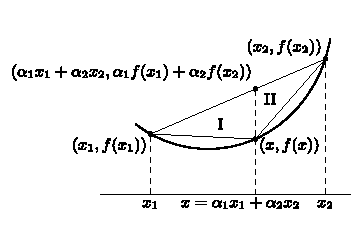
\includegraphics[width=8cm]{attachment/凸函数.pdf}
	\caption{凸函数示意图, 图源Zorich Fig. 5.11}
\end{figure}

凸函数的定义可以推广: 

\begin{theorem}{Jensen不等式}
	设$f:E \to \R$是凸函数, 其中$E$是区间. 则对任意$x_1,\cdots ,x_n \in E$和任意的$t_1,\cdots ,t_n \in [0,1]$, 如果$t_1+\cdots +t_n=1$, 则有
	\begin{center}
		$f(t_1x_1+\cdots +t_nx_n) \leq t_1f(x_1) + \cdots + t_nf(x_n). $
	\end{center}
\end{theorem}
\begin{proof}
	归纳即可. 
\end{proof}

\begin{proposition}{凸函数的等价条件}
	下列命题是等价的: 
	\begin{itemize}
		\item $f$在区间$E$上是凸函数. 
		\item 对于任意的$x,y,z \in E$, 若$x<y<z$, 则
		\begin{equation}
			\frac{f(y)-f(x)}{y-x} \leq \frac{f(z)-f(x)}{z-x} \leq \frac{f(z)-f(y)}{z-y}. \label{eq:凸函数等价定义}
		\end{equation}
		特别地, 若$f$是严格凸函数, 则上式中的不等号全部是严格的. 
		\item 集合$C=\{ (x,y):x\in E,y \geq f(x) \}$是凸集. 
	\end{itemize}
\end{proposition}
\begin{remark}
	若对任意$x,y \in C$和$t \in [0,1]$, $tx+(1-t)y \in C$, 则称$C$是凸集, 即是说$x,y$的连线仍在$C$中. 
\end{remark}
\begin{proof}
	(1) 若$f$是凸函数, 令$t=\frac{y-z}{x-z}$, 则$$f(y) = f(tx+(1-t)z) \leq tf(x)+(1-t)f(z) = \frac{y-z}{x-z}f(x) + \frac{x-y}{x-z}f(z).$$
	简单计算可知上式与式\ref{eq:凸函数等价定义}等价. 另一方面, 若式\ref{eq:凸函数等价定义}成立, 由$x,y,z$选取的任意性可知$f$是凸函数. 
\end{proof}

设$f$在$E$上可导. 我们注意到, 在式\ref{eq:凸函数等价定义}中令$y \to x$和$y \to z$, 有$$f'(x) \leq \frac{f(z)-f(x)}{z-x} \leq f'(z). $$
于是凸函数$f$的导数是单调不减的. 特别地, 若$f$是严格凸函数, 由Lagrange中值定理, 存在$x<\xi _1 < y < \xi _2 < z$使得$$f'(x) \leq f'(\xi _1) = \frac{f(y)-f(x)}{y-x} < \frac{f(z)-f(y)}{z-y} = f'(\xi _2) \leq f'(z).$$
于是$f$的导数是严格单调递增的. 

反过来, 用类似的方法可以证明, 若$f$的导数单调不减(严格单调递增), 则$f$是(严格)凸函数. 也就是说: 

\begin{proposition}{}
	设$E$是区间, $f:E \to \R$可导, 则$f$是(严格)凸函数当且仅当$f'$在$E$上单调不减(严格单调递增). 
\end{proposition}
\begin{remark}
	这个命题并不要求$f$存在二阶导数. 
\end{remark}

下面的命题说明, 就算没有$f$可导的假设, 凸性本身也可以诱导出分析的性质. 

\begin{proposition}{}
	设$E$是区间, $f:E \to \R$, 那么
	\begin{itemize}
		\item 对任意$x_0 \in \Int E$, $f$在$x_0$处的左右导数均存在(进而$f\in C(\Int E)$), 且$f'_-(x_0) \leq f'_+(x_0)$.
		\item 对任意$x,y \in \Int E$, 若$x<y$, 则
		\begin{center}
			$\displaystyle f'_-(x) \leq f'_+(x) \leq  \frac{f(y)-f(x)}{y-x} \leq f'_-(y) \leq f'_+(y).$
		\end{center}
	\end{itemize}
\end{proposition}
\begin{proof}
	(1) 由式\ref{eq:凸函数等价定义}可知对于$h_1,h_2>0$, $$\frac{f(x_0)-f(x_0-h_1)}{h_1} \leq \frac{f(x_0+h_2)-f(x_0)}{h_2}.$$
	特别地两侧分别关于$h_1,h_2$单调不减. 于是当$h_1 \to 0^-,h_2 \to 0^+$时, 两侧极限均存在, 且$f'_-(x_0) \leq f'_+(x_0)$. 
	
	(2) 同(1)可得$$\frac{f(x+h)-f(x)}{h} \leq \frac{f(y)-f(x)}{y-x}, $$
	在左侧令$h \to 0^+$, 即得$f'_+(x) \leq \frac{f(y)-f(x)}{y-x}$, 另一侧同理. 
\end{proof}

于是定义在闭区间上的凸函数只能在端点处不连续. 

另外, 既然$f$在每个点都存在左右导数, 我们可以研究左右切线: 

\begin{proposition}{}
	设$E$是区间, $f:E \to \R$是凸函数, $x_0 \in \Int E$, $\ell _k$表示过点$(x_0,f(x_0))$且斜率为$k$的直线. 则: 
	\begin{itemize}
		\item $f$的图像在$\ell _{f'_+(x_0)}$和$\ell _{f'_-(x_0)}$上方或重合. 
		\item $\ell _k$在$f$的图像之下或重合当且仅当$f'_-(x_0) \leq k \leq f'_+(x_0)$. 
	\end{itemize}
\end{proposition}
\begin{proof}
	(1) 以右极限情况为例, 只要证明对任意$x\neq x_0,x \in E$有$f(x) \geq f'_+(x_0)(x-x_0)+f(x_0)$, 当$x>x_0$时等价于$\frac{f(x)-f(x_0)}{x-x_0} \geq f'_+(x_0)$, 而这就是上方的命题. 当$x<x_0$时同理. 
	
	(2) 充分性显然. 必要性: 即当$x>x_0$时, $\frac{f(x)-f(x_0)}{x-x_0} \geq k$, 令$x \to x_0$即得$f'_+(x_0) \geq k$, 另一侧同理. 
\end{proof}

\begin{figure}[H]
	\centering
	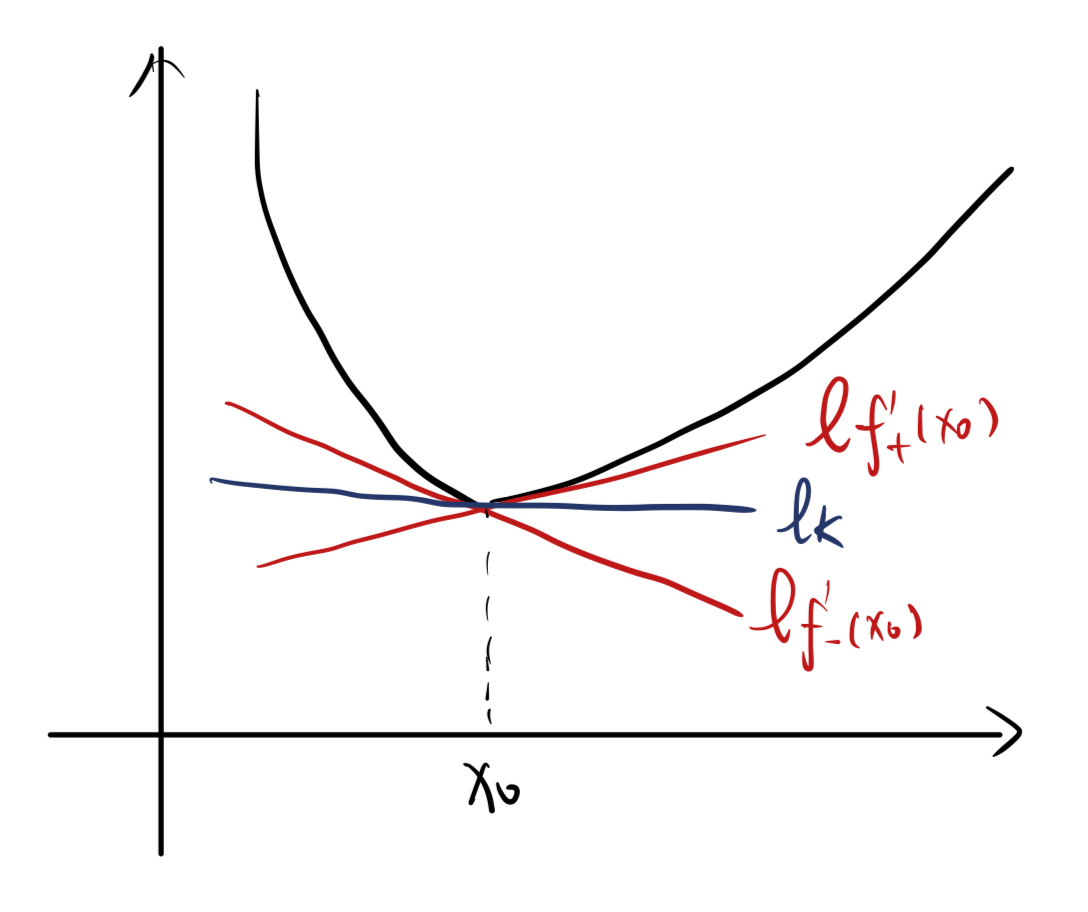
\includegraphics[width=6cm]{attachment/IMG_3552.jpg}
	\caption{凸函数的左右切线, 手绘勿喷}
\end{figure}

\newpage
\section*{一些习题 ~~\small 对应原书5.4习题} \label{sec:ex6.3}

\subsection*{A: 凸函数有关习题}

\circled{A1}~~设$f\in C((0,1))$, 且对任意$x_1,x_2 \in (0,1)$有$$f\left(\frac{x_1+x_2}{2} \right) \leq \frac{f(x_1)+f(x_2)}{2}$$
成立. 证明: $f$在$(0,1)$上是凸函数. 
\vspace{1em}

\circled{A2}-1~~若凸函数$f:\R \to \R$有界, 则它是常函数. 

\circled{A2}-2~~若凸函数$f:\R \to \R$满足$\lim_{x \to -\infty} \frac{f(x)}{x} = \lim_{x \to +\infty} \frac{f(x)}{x} =0$, 则它是常函数. 

\circled{A2}-3~~对于定义在$(a,+\infty)$上的任何凸函数$f$, 值$\frac{f(x)}{x}$在$x \to +\infty$时存在(广义)极限. 

\subsection*{B: 常用不等式的离散形式}

\circled{B1}~~(Young不等式) 设实数$a,b>0$和$p,q>1$, 满足$\frac{1}{p} + \frac{1}{q} =1$, 则有$$ab \leq \frac{a^p}{p} + \frac{b^q}{q},\qquad \textit{取等} \Leftrightarrow a^p=b^q.$$

\circled{B2}~~(Hölder不等式) 设实数$a_i,b_i>0$, 且$\frac{1}{p}+\frac{1}{q}=1$. 则当$p > 1$时有$$\sum_{k=1}^{n}(a_kb_k) \leq \left( \sum_{k=1}^{n} a_k^p \right)^{\frac{1}{p}} \left( \sum_{k=1}^{n} b_k^q \right)^{\frac{1}{q}},\qquad \textit{取等}\Leftrightarrow a_i^{p}=\lambda b_i^q. $$
当$0<p<1$时上述不等式反向. 取$p=q=2$, 即得Cauchy-Schwarz不等式. 
\vspace{1em}

\circled{B3}~~(Kantorovich不等式) 设实数$a_i,\lambda _i>0$, 且$\sum_{i=1}^{n}a_i=1$. 若$\lambda _i \in [m,M]$, 则有$$\left( \sum_{k=1}^{n} \lambda _k a_k \right) \left( \sum_{k=1}^{n} \frac{a_k}{\lambda _k} \right) \leq \frac{(m+M)^2}{4mM}.$$

\circled{B4}~~(Minkowski不等式) 设实数$a_i,b_i>0$. 当$p \geq 1$时有$$\left( \sum_{k=1}^{n} (a_k+b_k)^p \right)^{\frac{1}{p}} \leq \left( \sum_{k=1}^{n} a_k^p \right)^{\frac{1}{p}} + \left( \sum_{k=1}^{n} b_k^p \right)^{\frac{1}{p}},\qquad \textit{取等}\Leftrightarrow a_i=\lambda b_i.$$
当$0<p<1$时上述不等式反向. 

\newpage
\section{原函数与不定积分}

\begin{definition}{原函数}
	设$F$在区间$I$上可导. 称$F$为$f$在$I$上的一个\textit{原函数}(primitive function), 若$(F|_I)' = f|_I$. 
\end{definition}

由之前的命题, 不难证明$f(x)$在$I$上的所有原函数都是形如$F(x)+C$的形式. 于是可以定义:

\begin{definition}{不定积分}
	设$f$存在区间$I$上的原函数$F$, 则定义$f(x)$在$I$上的\textit{不定积分}(indefinite integration)为$$\int f(x) \dif x := \{ F(x)+C:C \in \R \}.$$
	亦可简写为$\int f(x) \dif x = F(x)+C$. 
\end{definition}

容易求得如下不定积分公式: 

\begin{figure}[H]
	\centering
	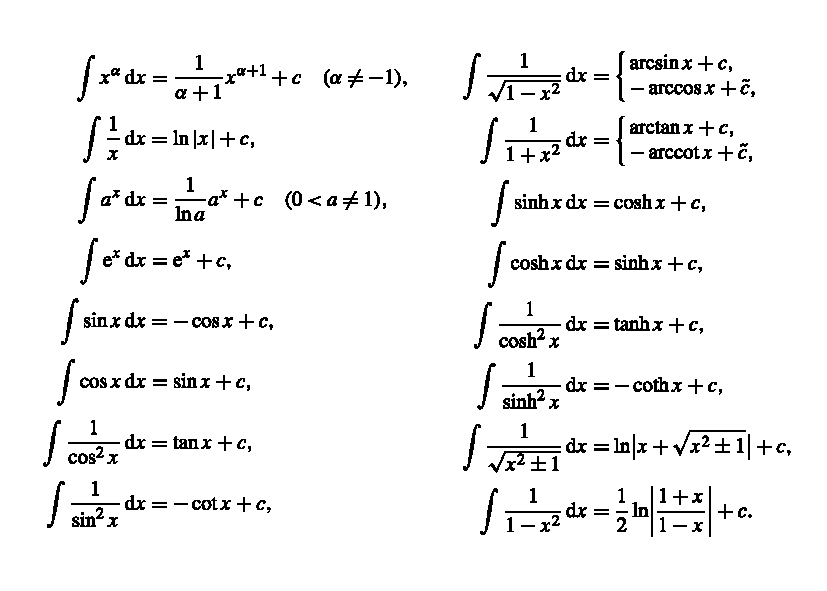
\includegraphics[width=14cm]{attachment/不定积分表.pdf}
	\caption{不定积分公式, 图源Zorich}
\end{figure}

利用微分的定义和性质, 还可以知道: 

\begin{proposition}{不定积分的简单性质}
	设$f$在区间$I$上的一个原函数$F$. 则: 
	\begin{itemize}
		\item $\displaystyle \dif \int f(x) \dif x = f(x) \dif x$. 
		\item $\displaystyle \int \dif F(x) = F(x) + C$. 
		\item $\displaystyle \int (\lambda f(x)+ \mu g(x)) \dif x = \lambda \int f(x) \dif x + \mu \int g(x) \dif x$. 
	\end{itemize}
\end{proposition}

下面介绍一些计算不定积分的公式和方法. 

\circled{A}~~换元积分法. 之前证明了$\dif v(u(x)) = v'(u(x)) \dif u(x)$. 在两侧同时求不定积分得$$\int \dif v(u(x)) = \int v'(u(x)) \dif u(x) \quad \Leftrightarrow \quad \int v'(u(x)) \dif u(x) = v(u(x)). $$

\begin{example}
	计算如下不定积分: $$1) \int \frac{x\dif x}{1+x^2};\qquad 2) \int \frac{\dif x}{\sin x}. $$
\end{example}
\begin{solution}
	(1) $$\int \frac{x\dif x}{1+x^2} = \frac{1}{2} \int \frac{\dif (1+x^2)}{1+x^2} = \frac{1}{2}\ln (1+x^2) +C.$$
	
	(2) $$\int \frac{\dif x}{\sin x} = \int \frac{\dif \frac{x}{2}}{\sin \frac{x}{2} \cos \frac{x}{2}} = \int \frac{\dif t}{\tan t \cos ^2 t} = \int \frac{\dif \tan t}{\tan t} = \ln \left| \tan \frac{x}{2} \right| + C.$$
\end{solution}

\circled{B}~~分部积分法: 之前证明了$\dif u(x)v(x) = (\dif u(x)) v(x) + u(x) (\dif v(x))$. 在两侧同时求不定积分得$$u(x)v(x) = \int v(x) \dif u(x) + \int u(x) \dif v(x). $$

\begin{example}
	计算如下不定积分: $$1) \int \ln x \dif x;\qquad 2) \int x^2e^x \dif x. $$
\end{example}
\begin{solution}
	(1) $$\int \ln x \dif x = x\ln x - \int e^{\ln x}\dif \ln x = x\ln x - x + C.$$
	
	(2) \begin{align*}
		\int x^2e^x \dif x &= \int x^2 \dif e^x = x^2e^x - \int e^x \dif x^2 = x^2e^x - 2\int xe^x \dif x \\
		&= x^2e^x - 2\int x \dif e^x = x^2e^x - 2\left( xe^x-\int e^x \dif x \right) = (x^2-2x+2)e^x + C. 
	\end{align*}
\end{solution}

\begin{example}
	计算如下不定积分: $$1) \int \cos (\ln x) \dif x;\qquad 2) \int \sin (\ln x) \dif x.$$
\end{example}
\begin{solution}
	计算可知$$\int \cos (\ln x) \dif x = \int x \dif \sin (\ln x) = x\sin (\ln x) - \int \sin (\ln x) \dif x,$$
	$$\int \sin (\ln x) \dif x = -\int x \dif \cos (\ln x) = -x\cos (\ln x) + \int \cos (\ln x) \dif x.$$
	于是$$\int \cos (\ln x) \dif x = \frac{1}{2}x(\sin (\ln x)+ \cos (\ln x)) +C,$$
	$$\int \sin (\ln x) \dif x = \frac{1}{2}x(\sin (\ln x)- \cos (\ln x)) +C.$$
\end{solution}

\circled{C}~~有理函数的不定积分. 我们熟知一个有理函数$\frac{P(x)}{Q(x)}$总是可以(在$\R$上)分解为一些形如$$\frac{1}{(x-a)^k},\qquad \frac{px+q}{(x^2+bx+c)^k}$$
的式子(其中$b^2<4c$)的线性组合. 于是只需要分别将两类式子的不定积分求出来: 
$$\int \frac{\dif x}{(x-a)^k} = \begin{cases}
	\frac{1}{-k+1}(x-a)^{-k+1}+C & k\neq 1 \\ \ln |x-a| + C & k=1
\end{cases}.$$
对于第二类, 令$u=x+\frac{b}{2}, a^2=c-\frac{b^2}{4}$, 于是$$\int \frac{px+q}{(x^2+bx+c)^k} \dif x = p \int \frac{u}{(u^2+a^2)^k} \dif u + \left(q-\frac{bp}{2} \right) \int \frac{\dif u}{(u^2+a^2)^k}.$$
其中$$\int \frac{u}{(u^2+a^2)^k} \dif u = \frac{1}{2} \int \frac{\dif (u^2+a^2)}{(u^2+a^2)^k} = \begin{cases}
	\frac{1}{2(1-k)}(u^2+a^2)^{1-k} & k\neq 1 \\ \frac{1}{2}\ln (u^2+a^2)
\end{cases}, $$
$$I_k = \int \frac{\dif u}{(u^2+a^2)^k} = \frac{u}{(u^2+a^2)^k} + 2k \int \frac{u^2}{(u^2+a^2)^{k+1}} \dif u = \frac{u}{(u^2+a^2)^k} + 2kI_k - 2ka^2I_{k+1}.$$
这样, 结合$$I_1 = \int \frac{\dif u}{u^2+a^2} = \frac{1}{a} \int \frac{\dif \frac{u}{a}}{1+(\frac{u}{a})^2} = \frac{1}{a} \arctan \frac{u}{a} + C,$$
我们就可以求出最终结果. 

\begin{example}
	计算如下不定积分: $$\int \frac{\dif x}{1+x^3}. $$
\end{example}
\begin{solution}
	注意到$1+x^3$的根为$-1,\frac{1+\sqrt{3}\ic}{2},\frac{1-\sqrt{3}\ic}{2}$, 于是不难求出$$\frac{1}{1+x^3} = \frac{\frac{1}{3}}{1+x} + \frac{-\frac{1}{3}x+\frac{2}{3}}{1-x+x^2}. $$
	现在开始计算: $$\int \frac{\dif x}{x+1} = \ln |x+1| + C,$$
	$$\int \frac{x-2}{x^2-x+1} \dif x = \int \frac{u-\frac{3}{2}}{u^2+\frac{3}{4}} \dif u = \frac{1}{2} \ln \left|u^2+\frac{3}{4} \right| -\sqrt{3} \arctan \left( \frac{2u}{\sqrt{3}} \right) + C.$$
	其中$u=x-\frac{1}{2}$. 所以$$\int \frac{\dif x}{1+x^3} = \frac{1}{3} \ln |x+1| - \frac{1}{6} \ln |x^2-x+1| + \frac{\sqrt{3}}{3}\arctan \left( \frac{2\sqrt{3}}{3}x-\frac{\sqrt{3}}{3} \right)+C.$$
\end{solution}

\circled{D}~~可有理化函数的不定积分. 

1. 设$R(u,v)=\frac{P(u,v)}{Q(u,v)}$. 为了将类似$R(\cos x,\sin x)$的式子变为关于$t$的有理函数, 我们可以利用如下换元: 
$$t=\tan \frac{x}{2},\qquad \int R(\cos x,\sin x) \dif x = \int R\left( \frac{1-t^2}{2t},\frac{2t}{1+t^2} \right) \frac{2\dif t}{1+t^2}, $$
$$t=\tan x,\qquad \int R(\cos ^2 x,\sin ^2 x) \dif x = \int R\left( \frac{1}{1+t^2},\frac{t^2}{1+t^2} \right) \frac{\dif t}{1+t^2}. $$
当然, 具体例题中常常使用其他三角变形公式和积分的换元公式来化简. 

\begin{example}
	计算如下不定积分: $$\int \frac{\dif x}{(\sin x + \cos x)^2}. $$
\end{example}
\begin{solution}
	\underline{\textbf{解法一}}~~令$t=\tan \frac{x}{2}$, 于是$$\int \frac{\dif x}{(\sin x + \cos x)^2} = \int \frac{\frac{2}{1+t^2}}{\left( \frac{2t}{1+t^2} + \frac{1-t^2}{1+t^2} \right)^2} \dif t = 2\int \frac{1+t^2}{(t^2-2t-1)^2} \dif t. $$
	之后利用有理函数的积分方法即可. 
	
	\underline{\textbf{解法二}}~~直接计算可得$$\int \frac{\dif x}{(\sin x + \cos x)^2} = \int \frac{\dif x}{\cos ^2x (1+\tan x)^2} = \int \frac{\dif \tan x}{(1+\tan x)^2} = -\frac{1}{1+\tan x}+C.$$
\end{solution}

2. 同上定义$R(u,v)$. 我们可做如下第二类化简: $$R\left( x,\sqrt[n]{\frac{ax+b}{cx+d}} \right) = R\left( \frac{dt^n-b}{-ct^n+a},t \right). $$
具体计算过于麻烦, 这里就不举例了. 

3. 同上定义$R(u,v)$. 考虑$R(x,\sqrt{ax^2+bx+c})$的情况. 实际上通过配方, 只需考虑如下三种简单形式: $$\int R(t,\sqrt{t^2+1}) \dif t, \qquad \int R(t,\sqrt{t^2-1}) \dif t, \qquad \int R(t,\sqrt{1-t^2}) \dif t. $$
Euler提出了针对这三种形式的代换: $$\sqrt{t^2+1}=tu\pm 1,t-u;\qquad \sqrt{t^2-1}=u(t\pm 1),t-u;\qquad \sqrt{1-t^2}=u(1\pm t),tu\pm 1. $$
右侧的式子都是可以取其相反数的. 当然另一种思路是利用三角/双曲换元. 
\begin{remark}
	考虑$R(x,\sqrt{P(x)})$的原函数, 其中$P(x)$是次数$n>2$的多项式. Abel和Liouville证明了这样的不定积分一般不能表示为初等函数. 我们称该积分在$n=3,4$时为\textit{椭圆积分}, 在$n>4$时为\textit{超椭圆积分}. 
\end{remark}

\begin{example}
	计算如下不定积分: $$\int \frac{\dif x}{x+\sqrt{x^2+2x+2}}. $$
\end{example}
\begin{solution}
	化简可得$$\int \frac{\dif x}{x+\sqrt{x^2+2x+2}} = \int \frac{\dif t}{t-1+\sqrt{t^2+1}}. $$
	其中$t=x+1$. 令$\sqrt{t^2+1}=u-t$, 于是$t=\frac{u^2-1}{2u}$, 进而$$\textit{原式} = \frac{1}{2} \int \frac{1+\frac{1}{u^2}}{u-1} \dif u = \int \frac{\dif u}{u-1} - \frac{1}{2} \int \frac{\dif u}{u^2} - \frac{1}{2} \int \frac{\dif u}{u} = \ln |u-1| - \frac{1}{2}\ln |u| + \frac{1}{2u} +C.$$
	其中$u=x+1+\sqrt{x^2+2x+2}$. 
\end{solution}


\newpage
\section*{一些习题 ~~\small 对应原书5.7习题} \label{sec:ex6.4}

\subsection*{A: 有理函数的积分}

设$\frac{P(x)}{Q(x)}$是有理真分式. 多项式$q(x)$的根与$Q(x)$的根相同且都是一重根. 记$Q_1(x)=\frac{Q(x)}{q(x)}$. 
\vspace{1em}

\circled{A1}-1~~证明Ostrogradskiy公式: $$\int \frac{P(x)}{Q(x)} \dif x = \frac{P_1(x)}{Q_1(x)} + \int \frac{p(x)}{q(x)} \dif x.$$
其中$\int \frac{p(x)}{q(x)}$是超越函数. $\frac{P_1(x)}{Q_1(x)}$称作原积分的有理部分. 
\vspace{1em}

\circled{A1}-2~~证明: 即使不知道多项式$Q(x)$的根, 也可以用代数方法求出$q(x),Q_1(x)$, 然后通过待定系数法求出$p(x),P_1(x)$. 因此, 即使不计算整个原函数, 也可以求出其有理部分. 
\vspace{1em}

\circled{A1}-3~~设$P(x)=2x^6+3x^5+6x^4+6x^3+10x^2+3x+2$, $Q(x)=x^7+3x^6+5x^5+7x^4+7x^3+5x^2+3x+1$. 求出$\int \frac{P(x)}{Q(x)} \dif x$的有理部分. 
\vspace{1em}

设待求的原函数为$\int R(\cos x,\sin x) \dif x$. 其中$R(u,v)$是有理函数. 
\vspace{1em}

\circled{A2}-1~~若$R(-u,v)=R(u,v)$, 则$R(u,v)$的形式为$R_1(u^2,v)$. 

\circled{A2}-2~~若$R(-u,v)=-R(u,v)$, 则$R(u,v)=uR_2(u^2,v)$, 进而代换$t=\sin x$可使积分有理化. 

\circled{A2}-3~~若$R(-u,-v)=R(u,v)$, 则$R(u,v)=R_3(\frac{u}{v} ,v^2)$, 进而代换$t=\tan x$可使积分有理化. 
\vspace{1em}

设待求的原函数为$\int R(x,\sqrt{ax^2+bx+c}) \dif x$. 

\circled{A3}-1~~用以下Euler代换可将其化为有理函数的积分: $$t=\sqrt{ax^2+bx+c}\pm \sqrt{a}x;\qquad t=\sqrt{\frac{a(x-x_1)}{x-x_2}}. $$
其中$x_1,x_2$是$ax^2+bx+c=0$的两根. 

\circled{A3}-2~~设$(x_0,y_0)$在曲线$y^2=ax^2+bx+c$上, 过该点的直线$\ell$交曲线于$(x,y)$, $t$是$\ell$的斜率. 指出这与Euler代换的联系. 

\circled{A3}-3~~若一条曲线$y(x)$由代数方程$P(x,y)=0$给出, 且它的参数方程$x=x(t),y=y(t)$均为有理函数, 则称其为\textit{有理曲线}. 证明: $\int R(x,y(x))$可化为有理函数积分. 

\circled{A4}-1~~求证: 微分二项式的积分$\int x^m(a+bx^n)^p \dif x$(其中$m,n,p \in \Q$)可以化为积分$$\int (a+bt)^pt^q \dif t~~(\textit{其中}p,q \in \Q).$$

\circled{A4}-2~~该积分可以表示为初等函数的一个充分条件是在$p,q,p+q$中有整数. (注: Chebyshev证明了这也是必要条件)



\subsection*{B: 椭圆积分}

\circled{B}-1~~设有理函数$R(u,v)$, $P$是三次或四次多项式, 则函数$R(x,\sqrt{P(x)})$可以化为$$R_1(t, \sqrt{at^4+bt^3+ct^2+dt+e}),$$其中$a \neq 0$. 
\vspace{1em}

\circled{B}-2~~设四次多项式$a(x^2+p_1x+q_1)(x^2+p_2x+q_2)$, 其可以通过代换$x=\frac{\alpha t+\beta}{\gamma t+1}$化为$$\dfrac{(M_1+N_1t^2)(M_2+N_2t^2)}{(\gamma t+1)^{4}} .$$
进而, 函数$R(x,\sqrt{ax^4+bx^3+cx^2+dx+e})$通过代换$x=\frac{\alpha t+\beta}{\gamma t+1}$化为$R_1(t,\sqrt{A(1+m_1t^2)(1+m_2t^2)})$. 
\vspace{1em}

\circled{B}-3~~任何函数$R(x,\sqrt{y})$都可以化为$R_1(x,y)+\frac{R_2(x^2,y)}{\sqrt{y}}+\frac{R_3(x^2,y)}{\sqrt{y}}x$的形式. 
\vspace{1em}

\circled{B}-4~~任何形如$\int R(x,\sqrt{P(x)}) \dif x$的积分, 其中$P(x)$是四次多项式, 在精确到相差初等函数时可化为积分$$\int \frac{r(t^2) \dif t}{\sqrt{A(1+m_1t^2)(1+m_2t^2)}} ,$$
其中$r(t)$是有理函数, $A=\pm 1$. 
\vspace{1em}

Í其中$0<k<1$, $\tilde{r}$是有理函数. 
\vspace{1em}

\circled{B}-6~~设$$I_n=\int \frac{x^{2n} \dif x}{\sqrt{(1-x^2)(1-k^2x^2)}},\qquad J_n = \int \frac{\dif x}{(x^2-a)^m\sqrt{(1-x^2)(1-k^2x^2)}}.$$
证明, $I_n$可用$I_0,I_1$表示, $J_n$可用$I_0,I_1,J_1$表示. 
\vspace{1em}

\circled{B}-7~~任何形如$\int R(x,\sqrt{P(x)}) \dif x$的积分, 其中$P(x)$是四次多项式, 在精确到相差初等函数时可化为以下三个标准椭圆积分: $$\int \frac{\dif x}{\sqrt{(1-x^2)(1-k^2x^2)}} ,\qquad \int \frac{x^2\dif x}{\sqrt{(1-x^2)(1-k^2x^2)}},\qquad \int \frac{\dif x}{(1+hx^2)\sqrt{(1-x^2)(1-k^2x^2)}},$$
其中$0<k<1$. 用$F(k,\varphi)$来表示使得$F(k,0)=0$的第一类椭圆积分, 用$E(k,\varphi)$来表示使得$E(k,0)=0$的第二类椭圆积分. 
\vspace{1em}







\newpage
\section{微分学的应用}

\subsection{对复数和幂级数的进一步研究}

我们知道多项式函数具有非常好的分析性质(即处处光滑), 那么作为其推广形式的幂级数是否存在同样的性质? 

\begin{theorem}{}
	设幂级数$f(z)=\sum_{k=0}^{\infty} c_k(z-z_0)^k$. 则$f(z)$在其收敛圆内处处光滑, 特别地$$1)~f^{(n)}(z) = \sum_{k=0}^{\infty} \frac{\dif ^n}{\dif z^n} (c_k(z-z_0)^k),\qquad 2)~c_k=\frac{f^{(k)}(z_0)}{k!}.$$
\end{theorem}
\begin{proof}
	只需证明1), 那么2)是自然的. 首先由Cauchy-Hadamard公式可知该式的收敛半径与$f(z)$相同, 记为$R$. 通过换元, 不妨设$z_0=0$. 利用归纳法, 只要证明$f'(z)=\sum_{k=1}^{\infty}c_kkz^{k-1}=:\varphi (z)$. 
	
	我们取$z_1,z_2$, 计算$$\left| \frac{f(z_1)-f(z_2)}{z_1-z_2} - \varphi (z) \right| = \left| \sum_{k=1}^{\infty} c_k(z_1^{k-1}+ z_1^{k-2}z_2 + \cdots + z_1z_2^{k-2} + z_2^{k-1}) - \sum_{k=1}^{\infty} c_kkz^{k-1} \right|.$$
	由于上面两个级数均收敛(将$|z_1|$放缩为$R$立得), 取$N$使得它们与前$N$项之和的差能被$\varepsilon$控制住, 即$$\left| \frac{f(z_1)-f(z_2)}{z_1-z_2} - \varphi (z) \right| \leq 2\varepsilon + \left| \sum_{k=1}^{N} c_k(z_1^{k-1} + \cdots + z_2^{k-1} - kz^{k-1}) \right|.$$
	令$z_1,z_2 \to z$, 则显然上述不等式右侧趋于$0$, 即得原命题成立. 
\end{proof}

一般地, 若函数$f(z)$在$z_0$的某个邻域内可以表示为幂级数的形式, 则称$f(z)$在$z_0$\textit{解析}. 由上面的定理可知, 此时$f$在$z_0$处光滑. (实际上可以证明, 若$f$在$z_0$附近可微, 则在$z_0$解析)

\begin{theorem}{代数基本定理}
	每个$n$次复系数多项式$p(z)=c_0+\cdots +c_nz^n$在$\C$中都有根. 
\end{theorem}
\begin{remark}
	进一步, 容易说明: $p(z)$在$\C$上恰有$n$个根. 
\end{remark}
\begin{proof}
	由于$p$连续, 存在点$z_0$使得$|p(z_0)|=\inf_{z \in \C}|p(z)|$. 下面证明$p(z_0)=0$: 设若不然, 考虑多项式$q(z)=\frac{p(z+z_0)}{p(z_0)}$, 那么$q(0)=1$, $1= |q(0)|=\inf_{z \in \C} |q(z)|$. 记$q(z)=1+a_kz^k+\cdots +a_nz^n$, 其中$a_k \neq 0$. 令$a_k=re^{\ic \theta}$, $\beta ^k = \rho ^k e^{\ic (\pi-\theta)}$, 那么当$\rho$足够小时, $$|q(\beta)| \leq |1+a_k\beta ^k| + (|a_{k+1}\beta ^{k+1}| + \cdots + |a_n\beta ^n|) = 1-\rho ^k(r-\rho |a_{k+1}|-\cdots -\rho ^{n-k}|a_n|) <1.$$
	这与$|q(z)| \geq 1$矛盾! 
\end{proof}

\subsection{简单的常微分方程}

\begin{definition}{常微分方程}
	设关于$x$的函数$y$, $y$存在$n$阶导数, 则称系统$$f\left( x,\frac{\dif ^n y}{\dif x^n},\cdots ,\frac{\dif y}{\dif x},y \right)=0$$
	为一个\textit{常微分方程}(ordinary differential equation), 其中$y$称为该方程的解. 
\end{definition}

下面介绍一些简单的常微分方程及其解法. 

\circled{A}~~变量分离方程. 

\begin{example}
	(有空气阻力的自由落体) 质量为$m$的小物块从静止开始自由落体, 设其受到的空气阻力$f$与速度$v$成正比, 求$v$关于时间$t$的表达式. 
\end{example}
\begin{solution}
	由Newton第二定律, $$m \frac{\dif v}{\dif t} =mg-kv \quad \Leftrightarrow \quad \frac{\dif v}{g-\frac{k}{m} v} = \dif t.$$
	两边同时积分得, $$-\frac{m}{k} \ln \left(g-\frac{k}{m}v \right)+C=t.$$
	即$v=\frac{m}{k}(g-e^{-\frac{k}{m}t+C_1})$. 特别地$t=0$时$v=\frac{m}{k}(g-e^{C_1}))=0$, 从而解得$C_1=\ln g$. 所以
	\begin{center}
		$\displaystyle v = \frac{mg}{k}(1-e^{-\frac{k}{m}t}).$
	\end{center}
\end{solution}

\begin{example}
	(简谐振动) 质量为$m$的小物块从平衡位置$x=0$以速度$v_0$开始振动, 始终受到一个指向平衡位置的力$F=-kx$, 这里的位移$x$定义为平衡位置到当前位置的矢量. 求位移$x$关于时间$t$的表达式. 
\end{example}
\begin{solution}
	由Newton第二定律, $$m \frac{\dif ^2x}{\dif t^2} = -kx \quad \Leftrightarrow \quad m \frac{\dif v}{\dif x} \frac{\dif x}{\dif t} = -kx \quad \Leftrightarrow \quad mv\dif v=-kx\dif x.$$
	两侧(定)积分, 有$\frac{1}{2}mv^2-\frac{1}{2}mv_0^2 = -\frac{1}{2}kx^2$, 即$$\frac{\dif x}{\dif t} = \sqrt{v_0^2-\frac{k}{m}x^2} \quad \Leftrightarrow \quad \frac{\dif x}{\sqrt{v_0^2-\frac{k}{m}x^2}} = \dif t.$$
	两侧积分, 有$\arcsin (\sqrt{\frac{k}{m}} \frac{x}{v_0}) = \sqrt{\frac{k}{m}} t+C$, 容易求得$$x = v_0\sqrt{\frac{m}{k}}\sin \left( \sqrt{\frac{k}{m}}t \right).$$
\end{solution}

\circled{B}~~一阶线性方程, 即形如$y' + p(x)y=q(x)$的微分方程. 记$\int p = P, \int q = Q$. 

当$q(x)=0$时, 即齐次情况, 容易求得$y=Ce^{-P(x)}$. 当$q(x)$不恒等于$0$时, 希望找到类似$(\mu (x) y)'=q(x)\mu (x)$的形式(这是所谓恰当方程的形式), 即只需$\frac{\mu '(x)}{\mu (x)} = p(x)$, 可得$\mu (x) = e^{P(x)}$. 由此有$$y=e^{-P(x)}\left( \int e^{P(x)}q(x) \dif x + C \right).$$
我们也可以用所谓常数变易法求解该方程, 即待定$y=C(x)e^{-P(x)}$之后代回计算. 

\circled{C}~~高阶常系数齐次线性方程, 即形如$y^{(n)}+a_1y^{(n-1)} + \cdots + a_{n-1}y'+a_ny=0$的微分方程. 

令$y_1=y,\cdots ,y_n=y^{(n-1)}$, $y=(y_1,\cdots ,y_n)$, 上述式子就等价于求解$$\frac{\dif y}{\dif x} = Ay,\qquad A=\begin{pmatrix}
  & 1 &  &  &   \\
  &  & 1 &  &   \\
  &  &  & \ddots    & \\
  &  &  &    & 1\\
 -a_n & -a_{n-1} & -a_{n-2} & \cdots  & -a_1
\end{pmatrix}.$$
熟知$A$的特征多项式为$\lambda ^n+a_1\lambda ^{n-1} + \cdots + a_{n-1}\lambda +a_n=0$, 记$A$的特征值为$\lambda _1,\cdots ,\lambda _t$, 对应代数重数$n_1,\cdots ,n_t$. 则$$e^{\lambda _ix},\quad xe^{\lambda _ix}, \quad \cdots \quad x^{n_i-1}e^{\lambda _ix},\qquad i=1,\cdots ,t$$
构成该方程的一个基本解组(证明略). 

\begin{example}
	(阻尼振动) 质量为$m$的小物块从平衡位置$x=0$以速度$v_0$开始振动, 始终受到一个指向平衡位置的动力$F=-kx$和一个与运动方向相反的阻力$f=-r v$. 求位移$x$关于时间$t$的表达式. 
\end{example}
\begin{solution}
	由Newton第二定律, $mx''+rx'+kx=0$, 对应特征方程$m\lambda ^2+r\lambda +k=0$. 
	
	当$\Delta = r^2-4mk>0$时, 设两个实特征值为$\lambda _1,\lambda _2$, 则$$x=C_1e^{\lambda _1t}+C_2e^{\lambda _2t}.$$
	
	当$\Delta = r^2-4mk=0$时, 有$2$-重特征值$-\frac{r}{2m}$, 则$$x=(C_1+C_2t)e^{-\frac{r}{2m}t}.$$
	
	当$\Delta = r^2-4mk<0$时, 两个复特征值为$\lambda_{1,2}=\frac{-r\pm \ic \sqrt{-\Delta}}{2m}$, 因此$$x=e^{-\frac{r}{2m}t}\left( C_1\cos \left( \frac{\sqrt{-\Delta}}{2m}t \right)+C_2\sin \left( \frac{\sqrt{-\Delta}}{2m}t \right) \right).$$
\end{solution}











































\chapter{Riemann积分}

\section{Riemann可积的定义}

我们先来看一个例子: 尝试计算(定义)抛物线$y=x^2,0\leq x \leq 1$与$x$轴围成的面积. 一种自然的思路是利用矩形进行逼近, 因为我们可以简单地定义出矩形的面积. 具体来说, 考虑$[0,1]$区间的一个分割$\pi = \{ 0=x_0<x_1<\cdots <x_{n-1}<x_n=1 \}$, 并在每个小区间内部取点$\xi _i \in [x_{i-1},x_i]$, 记$\xi = \{ \xi _1,\cdots ,\xi _n \}$. 我们希望定义如下的极限就是所求面积: $$\lim_{\| \pi \| \to 0} \sum_{i=1}^{n}(x_i-x_{i-1})\xi _i^2. $$
其中, 极限过程$\| \pi \| \to 0$的意思是$\max_{1\leq i \leq n} \{x_i-x_{i-1}\} \to 0$(这的确构成一种极限过程, 后面会证明). 

这种定义有非常明显的问题: 
\begin{itemize}
	\item 分割$\pi$和标记点$\xi$并不确定, 因而无法很方便地计算这个极限. 
	\item 由于不便将该式化简, 我们甚至不知道这样的极限是否存在. 
\end{itemize}
针对这两个问题, 可能会有如下想法: 
\begin{itemize}
	\item 用平均分割和统一的标记点选取标准来代替一般化的方法. 注意这种计算方式一定是充分条件. 
	\item 类似于数列, 既然难以判断极限是否存在, 可以考虑定义上下极限来逼近. 
\end{itemize}
综合这两种想法, 在本例中我们可以如下考察所求的面积: 首先取平均分割$\pi_{n}=\{ x_i=\frac{i}{n} \}$, 接着选择两种不同的标记点集$\displaystyle\xi _L = \big\{ \xi _i :  \xi _i ^2= \inf_{x_{i-1} \leq x \leq x_i} x^2 \big\}$, $\displaystyle\xi _U = \big\{ \xi _i : \xi _i ^2= \sup_{x_{i-1} \leq x \leq x_i} x^2 \big\}$. 考虑极限过程$n\to \infty$, 于是两种极限$S_L$和$S_U$就是: $$S_L = \lim_{n\to \infty} \left( \frac{1}{n} \sum_{i=1}^{n} \frac{(i-1)^2}{n^2} \right) = \lim_{n\to \infty} \frac{2n^2-3n+1}{6n^2} = \frac{1}{3} ,  $$
$$S_U = \lim_{n\to \infty} \left( \frac{1}{n} \sum_{i=1}^{n} \frac{i^2}{n^2} \right) = \lim_{n\to \infty} \frac{2n^2+3n+1}{6n^2} = \frac{1}{3}.$$
注意到$S_L=S_U = \frac{1}{3}$, 于是所求面积(似乎)就是$\frac{1}{3}$. 

上面的例子就是利用Riemann和进行逼近计算(定义)的做法. 我们不难想到另一种方法: 先定义所谓阶梯函数(这种函数的积分易于定义), 再考虑找到特定函数的阶梯函数逼近, 最后计算极限阶梯函数的积分即可. 这两种方法本质上是相同的, 只是操作顺序不一样. 然而利用后者有两个优势: 我们能够自然地理解Riemann积分的某些缺陷(例如只能处理有界函数), 另外实际上Riemann和的定义无法推广到$\R ^n$上(依赖序关系). 


\subsection{阶梯函数及其积分}

首先我们考虑\textit{示性函数}(characteristic function): 设$E \subseteq \R$, 则定义$$\chi _{E}:\R \to \{ 0,1 \},\quad \chi _{E} (x) = \begin{cases}
	1 & x \in E \\ 0 & x \notin E
\end{cases}.$$
我们希望定义$\chi _E$的积分, 而这自然需要定义集合$E$的长度. 我们不希望引入繁杂的测度理论, 于是承认下方的“公理”: 对于某个将集合映射到其对应长度的函数$\mu$, 我们希望有$$\mu ((a,b)) = \mu ([a,b]) = \mu ([a,b)) = \mu ((a,b]) = b-a, $$
$$\mu ((-\infty ,+\infty)) = \mu ((-\infty ,b)) = \mu ((a ,+\infty)) = +\infty .$$
第一行的“公理”也在告诉我们: 像$a,b$这样的点是没有长度的. 

于是, 我们可以定义示性函数的\textit{积分}(integral)为$$\int \chi _E := \mu (E). $$
特别地, $$\int \chi _{(a,b)} = \int \chi _{[a,b]} = \int \chi _{[a,b)} = \int \chi _{(a,b]} = b-a. $$
当然, 实际定义阶梯函数的积分时只需要用到$E$是区间的情况, 因此上方不严谨的思考并不影响结果的正确性. 

接下来看\textit{阶梯函数}(更多时候称为\textit{简单函数}, simple function): 

\begin{definition}{分划, 阶梯函数, 阶梯函数的积分}
	设闭区间$I=[a,b]$. 
	\begin{itemize}
		\item 称形如$$\pi = \{ a=x_0<x_1<\cdots <x_{n-1}<x_n=b \}$$
		的集合为$I$的一个\textit{分划}(partition). 
		\item 定义分划$\pi$的\textit{步长}(step): $$\| \pi \| := \max_{1 \leq i \leq n} \{ x_i-x_{i-1} \}. $$
		\item 对于分划$\pi= \{ a=x_0<\cdots <x_n=b \}$, 称形如$$f = \sum_{i=1}^{n} \lambda _i \chi _{(x_{i-1},x_{i})} $$
		(其中$\lambda _i \in \R$)的函数为$\pi$上的一个\textit{阶梯函数}. 记$I$上全体阶梯函数的集合为$\mathcal{S}(I)$. 
		\item 承上一条, 定义$f$的\textit{积分}(integral)为$$\int f := \sum_{i=1}^{n} \lambda _i \int \chi _{(x_{i-1},x_i)} = \sum_{i=1}^{n} \lambda _i (x_i-x_{i-1}). $$
	\end{itemize}
\end{definition}
\begin{remark}
	刚才说过, 点是没有长度的, 因此阶梯函数在分割点处的取值应当对最终结果没有影响. 
\end{remark}
\begin{remark}
	为了避免与原函数的符号相混淆, 也记$\int f = \int _I f = \int_a^b f$. 不过为了方便, 我们暂时混用这些符号. 
\end{remark}

这里, 我们实际上需要验证阶梯函数积分的良定义性. 也就是说, 如果$\pi, \pi '$均与$f$相容, 则$f$依这两种分划的积分相等. 一般地, 我们称$\pi ' \prec \pi$($\pi '$比$\pi$细), 如果$\pi$的分割点都是$\pi '$的分割点. 于是我们只需要验证, 若$\pi ' \prec \pi$, 则$f$依这两种分划的积分相等(这是因为我们可以取$\overline{\pi} = \pi \cup \pi '$). 而这是显然的. 

接下来研究积分算子的性质: 

\begin{proposition}{阶梯函数积分算子的性质}
	设闭区间$I=[a,b]$. 设$f,g \in \mathcal{S}(I)$. 则$\int : \mathcal{S}(I) \to \R$满足: 
	
	a) 线性: $$\int (\lambda f+ \mu g) = \lambda \int f + \mu \int g.$$
	
	b) 区间可加性: 设$I=[a,c] \cup [c,b]$, 则$$\int_a^b f = \int_a^c f + \int_c^b f. $$
	
	c) 三角不等式: $$\left| \int f \right| \leq \int |f|. $$
	
	d) 保号性/保序性: 若$f \geq 0$, 则$$\int f \geq 0. $$
	\qquad 特别地, 若$f \leq g$, 则$$ \int f \leq  \int g.$$
	
	e) 对积分的估计: 选取与$f$相容的分划$\pi= \{ a=x_0<\cdots <x_n=b \}$后, $$\left| \int_a^b f \right| \leq |b-a| \sup_{1 \leq i \leq n} |\lambda _i|. $$
\end{proposition}
\begin{proof}
	注意到阶梯函数是有限求和, 诸命题的验证就是显而易见的了. 
\end{proof}

\subsection{Riemann可积的定义}

现在来对一般函数定义Riemann积分. 首先是从阶梯函数角度出发: 

\begin{definition}{Riemann可积}
	设闭区间$I=[a,b]$. 称$f$是\textit{Riemann可积的}, 如果对任意$\varepsilon >0$均存在$F,e \in \mathcal{S}(I)$使得$$\forall x \in I,|f(x)-F(x)|<e(x),\qquad \int e < \varepsilon .$$
	全体$I$上Riemann可积的函数构成集合$\mathcal{R}(I)$. 
\end{definition}


我们需要对上述定义中的$F$逐个求积分并取其“极限”. 从上方的定义, 我们不难想到类似于序列逼近函数极限的思路: 考虑某种意义上的一列逼近函数$\{ f_n \}$, 然后定义$$\int f := \lim_{n\to \infty} \int f_n.$$

\begin{proposition}{} \label{pro:jptihjuudgjxdkyi}
	设闭区间$I=[a,b]$. 则下列说法等价: 
	\begin{itemize}
		\item $f$是Riemann可积的. 
		\item 存在阶梯函数序列$\{ f_n \},\{ e_n \}$使得$$\forall x \in I,|f(x)-f_n(x)|<e_n(x),\qquad \lim_{n\to \infty} \int e_n = 0.$$
		并且令$$\int f := \lim_{n\to \infty} \int f_n .$$
	\end{itemize}
\end{proposition}
\begin{proof}
	1) $\Rightarrow$ 2): 对任意$n>0$, 存在$f_n$使得$|f(x)-f_n(x)|<e_n(x)$使得$\int e_n < 1/n$, 从而$\lim_{n\to \infty} \int e_n = 0$. 

	2) $\Rightarrow$ 1): 显然. 

	另外, 我们还需证明$\int f = \lim_{n\to \infty} \int f_n$是良定义的, 即极限存在且不依赖于$\{ f_n \}$的选取: 

	由于$|f_n(x)-f_m(x)| \leq |f(x)-f_n(x)| + |f(x)-f_m(x)| \leq e_n(x)+e_m(x)$, 在两边积分可得$$\left| \int f_n-\int f_m \right| \leq \int |f_n-f_m| \leq \int e_n + \int e_m \to 0.$$
	这说明$\{ \int f_n \}$是Cauchy列, 进而存在极限. 

	另一方面, 设有另外的$\{ f'_n \}$和$\{ e'_n \}$符合要求, 则$|f_n(x)-f'_n(x)| \leq |f(x)-f_n(x)| + |f(x)-f'_n(x)| \leq e_n(x)+e'_n(x)$, 两侧积分可得$$\left| \int f_n - \int f'_n \right| \leq \int |f_n-f'_n| \leq \int e_n+ \int e'_n \to 0.$$
	于是两个极限相等. 
\end{proof}


类似于阶梯函数积分算子的性质, 对一般的积分算子也有如下性质: 

\begin{proposition}{} \label{pro:jiffxkvi1}
	设闭区间$I=[a,b]$. 设$f,g \in \mathcal{R}(I)$. 则$\int : \mathcal{R}(I) \to \R$满足: 
	
	a) 线性: $$\int (\lambda f+ \mu g) = \lambda \int f + \mu \int g.$$
	
	b) 区间可加性: 设$I=[a,c] \cup [c,b]$, 则$$\int_a^b f = \int_a^c f + \int_c^b f. $$
	
	c) 三角不等式(注意这依赖于$|f|$的可积性, 当然证明是显然的): $$\left| \int f \right| \leq \int |f|. $$
	
	d) 保号性/保序性: 若$f \geq 0$, 则$$\int f \geq 0. $$
	\qquad 特别地, 若$f \leq g$, 则$$ \int f \leq  \int g.$$
	
	e) 对积分的估计: 选取与$f$相容的分划$\pi= \{ a=x_0<\cdots <x_n=b \}$后, $$\left| \int_a^b f \right| \leq |b-a| \sup_{a \leq x \leq b} |f(x)|. $$
\end{proposition}
\begin{remark}
	尽管无法给出$\int fg$关于$\int f,\int g$的表达式, 我们仍然希望证明$fg$是可积的. 然而, 正是由于$\int fg$不好表示, 这里无法证明. 在下一节我们会处理这个问题. (实际上用阶梯函数的确能处理, 只不过太麻烦)
\end{remark}

接着从Riemann和角度出发. 类似于前文的例子, 如下定义: 基于分割点集$\pi$和标记点集$\xi$, 则$f$的\textit{Riemann和}为: $$S(f;\pi ,\xi) := \sum_{i=1}^{n} (x_i-x_{i-1})f(\xi _i) .$$
对于取定的函数$f$, 定义它的基为$\mathcal{B} := \{ B_{\delta}:\delta >0 \}$, 其中$B_{\delta} := \{ (\pi ,\xi) : \| \pi \|< \delta \}$. 不难证明, 这的确是一个基. 

\begin{proposition}{}
	设闭区间$I$, $f$在$I$上Riemann可积, 则
	\begin{center}
		$\displaystyle \lim_{\mathcal{B}} S(f;\pi ,\xi) = \int_I f.$
	\end{center}
\end{proposition}
\begin{proof}
	任取$\varepsilon >0$, 设阶梯函数$F,e$使得$|f(x)-F(x)|<e(x)$且$\int e(x) < \varepsilon$, 且不妨设$F,e$的分割点集均为$\pi _0 =\{ a=x_0<\cdots <x_n=b \}$. 待定分割点集$\pi = \{ a=y_0<\cdots <y_m=b \}$和与之对应的任意标记集$\xi$. 令$\| \pi \| < \min_{1 \leq i \leq n} \{ x_i-x_{i-1} \}$, 于是$$\left| S(f;\pi ,\xi) - \int_I f \right| \leq \sum_{i=1}^{m} \left| f(\xi _i)-\int_{y_{i-1}}^{y_i} f \right|. $$
	我们基本的思路是控制住$|(y_i-y_{i-1})f(\xi _i)-\int_{y_{i-1}}^{y_i}|$. 比较容易的方法是将$|f(x)|$放缩为其上界$M$, 从而该式不超过$2M(y_i-y_{i-1})$. 然而, 若将其累加, 最后无法得到可用$\| \pi \|$控制的极限. 因此, 希望这种(无可奈何的)放缩尽可能少. 特别地, 注意到那些使得$(y_{i-1},y_i) \subseteq (x_{j-1},x_j)$的区间可用$\varepsilon$放缩, 而剩下的区间不超过$n$个(为什么?), 这些区间采用刚才的放缩就是可以容忍的. 因此, 对$i$, 分情况讨论: 
	
	若$(y_{i-1},y_i)$完全包含在某个$(x_{j-1},x_j)$中: 易知$|f(x)-f(\xi _i)| \leq |f(x)-F(x)| + |F(\xi _i)-f(\xi _i)| \leq e(x)+e(\xi _i)$, 
	从而$$\left| (y_i-y_{i-1})f(\xi _i)-\int_{y_{i-1}}^{y_i} f \right| \leq 2\int_{y_{i-1}}^{y_i} e.$$
	
	若$(y_{i-1},y_i)$恰包含某个$x_j$: 由$f$可积知$f$有界, 设$|f(x)|<M$. 此时有$$\left| (y_i-y_{i-1})f(\xi _i)-\int_{y_{i-1}}^{y_i} f \right| \leq 2(y_i-y_{i-1})M \leq 2\| \pi \|M.$$
	
	综上可得, $$\left| S(f;\pi ,\xi) - \int_I f \right| \leq 2\sum_{i=1}^{m} \int_{y_{i-1}}^{y_i} e + 2n\| \pi \|M \leq 2\varepsilon + 2nM\| \pi \|.$$
	先令$\| \pi \|\to 0$, 则$\limsup_{\| \pi \|\to 0} LHS \leq 2\varepsilon$. 再令$\varepsilon \to 0$即得. 
\end{proof}


\subsection{非负函数的积分, 连接阶梯函数与Riemann和的途径}

从坐标图上来看, 将$f$拆分为非负部分$f^+$和非正部分$f^-$再分别计算两部分的积分似乎是一个可行的方法, 即令$f=f^+-f^-$, 之后定义非负函数$g$的积分为$$\int g := \sup \left\{ \int G:0\leq G \leq g, G \in \mathcal{S}(I)  \right\}, $$
最后令$\int f = \int f^+ - \int f^-$. 

我们先来研究最简单的情形, 即$f$本身就是非负函数: 

\begin{proposition}{} \label{pro:fwfuhjuubijb}
	设闭区间$I=[a,b]$, $f \geq 0$. 则在下列说法中, 1)可以推出2), 而2)加上条件$$\sum_{i=1}^{\ell} \omega (f,(x_{i-1},x_i)) (x_i-x_{i-1}) \to 0,\quad \| \pi \| \to 0$$可以推出1). 
	\begin{itemize}
		\item $f$是Riemann可积的. 
		\item $f$有界, 则集合$$\mathcal{A} = \left\{ \int F:0\leq F \leq f, F \in \mathcal{S}(I)  \right\}$$
		有界. 进而$\sup \mathcal{A}$存在, 令$$\int f := \sup \mathcal{A}.$$
	\end{itemize}
\end{proposition}
\begin{proof}
	(1) 应用上个命题的等价条件, 由于阶梯函数都有界, 显然$f$有界. 下证$\lim_{n\to \infty} \int f_n = \sup \mathcal{A}$. 假设该式不成立, 即存在$M,\varepsilon$使得$\lim_{n\to \infty} \int f_n < M < M+\varepsilon < \sup \mathcal{A}$, 于是对足够大的$n$均有$\int f_n < M$, 且存在阶梯函数$0\leq F \leq f$使得$\int F > M+\varepsilon$. 这就是说, $$e_n(x) > f(x)-f_n(x) \geq F(x)-f_n(x).$$
	两侧(均为非负的阶梯函数)同时积分, 即得$\int e_n(x) \geq \int F(x) - \int f_n(x) > \varepsilon >0$, 矛盾. 因此$\lim_{n\to \infty} \int f_n = \sup \mathcal{A}$. 
	
	(2) 对于$\mathcal{S}(I) \ni F,F' \geq 0$, 定义$F,F'$等价当且仅当它们的分割点集是一样的. 在每个等价类$[F]$中, 设分割点集为$\pi$, 定义该等价类的“极大项”为$$\varphi ([F]) := \sum_{i=1}^{n} \inf_{(x_{i-1},x_i)} f \cdot \chi _{(x_{i-1},x_i)}.$$
	显然$\tilde{\mathcal{A}}:=\{ \int \varphi ([F]):\mathcal{S}(I) \ni F \geq 0 \}$是$\mathcal{A}$的子集, 且$\sup \tilde{\mathcal{A}} = \sup \mathcal{A}$(为什么?). 于是取$\{ \varphi _n \} \subseteq \{ \varphi ([F]):\mathcal{S}(I) \ni F \geq 0 \}$使得$\int \varphi _n \nearrow \sup \mathcal{A}$. 这样的$\varphi _n$与其分割集$\pi _n$是一一对应的关系. 若$\int \varphi _m > \int \varphi _n$, 考虑$\tilde{\pi} = \pi _n \cup \pi _m$, 则$\tilde{\pi}$所对应的$\varphi$(不一定在该序列中)满足$\int \varphi \geq \int \varphi _m$, 将其添加到序列中. 于是我们不妨设该序列存在一个子列$\{ \varphi _{k_n} \}$, 使得对任意$n>0$, $\varphi _{k_{n+1}}$的分割点集都比$\varphi _{k_{n}}$的分割点集细. 令$$e_{k_n} = \sum_{i=1}^{\ell} \omega (f,(x_{i-1},x_i)) \chi _{(x_{i-1},x_i)}, $$
	其中$e_{k_n}$与$\varphi _{k_n}$的分割点集相同. 那么$f(x)-\varphi _{k_n}(x) \leq e_{k_n}(x)$. 最后, 利用命题中给出的条件, $$\int e_{k_n} = \sum_{i=1}^{\ell} \omega (f,(x_{i-1},x_i)) (x_i-x_{i-1}) \to 0, \quad \| \pi \| \to 0. $$
	这就是说$\int e_{k_n} \to 0,n \to \infty$. 
\end{proof}
\begin{remark}
	从该命题的证明中, 我们发现通过一个特殊的序列$\{ \varphi _{k_n} \}$, 可以将阶梯函数(“$n\to \infty$”)与Riemann和(“$\| \pi \|\to 0$”)联系起来. 这一思路会在下一小节会有体现. 
\end{remark}
\begin{remark}
	这个命题(加上后面的推论)实际上只是证明了该条件加上有界性可以得到可积性. 后面会证明可积函数有界且满足该条件. 
\end{remark}
\begin{remark}
	从(2)的证明可以看出Riemann积分并不够好, 因为我们需要人为添加一个条件才能保证可积. 
\end{remark}


接着看一般情况: 

\begin{corollary}{} \label{cor:fwfuhjuujiff}
	将上面命题的$f \geq 0$这一条件去掉, 并重新定义$\int f$如下, 原来的两条结论仍成立: 取$f^+ := \max \{ f,0 \}, f^{-} := \max \{ -f,0 \}$, 则$f=f^+-f^-$. 令$\int f = \int f^+ - \int f^-$. 
\end{corollary}
\begin{proof}
	实际上只用证明: $f$可积当且仅当$f^+,f^-$均可积. 
	
	(1) 必要性: 将$f$对应的阶梯函数按照$f$的零点切割, 显然可得. 
	
	(2) 充分性: 类似必要性, 当$f$的零点有限时显然. 若零点并非有限, 则直接拼接起来的“阶梯函数”不一定是有限求和, 故而我们需要合理舍弃一些段. 
	
	利用聚点定理, 找到零点集合的所有聚点, 对每个聚点$p$考虑其邻域$U_p$, 显然$U = \bigcup_{p\textit{是聚点}} (U_p \cap I) $是闭集, 且$U^c$是有限集合(容量为$n$). 由有限覆盖定理, 存在有限个($m$个)$U_{p_i}$使得$U=\bigcup_{i=1}^{n} U_{p_i}$. 
	
	选取在$U^c$中的($n$个)段, 将这些段上的阶梯函数拼接起来, 其余部分以$0$填充. 由上方的论述, 通过合并端点位于同一个$U_{p_i}$中的段, 存在$m$个段$I_1,\cdots ,I_m$恰好对应其余部分. 因此完整的的阶梯函数与$f$的误差之积分不超过$\varepsilon _1 + \cdots + \varepsilon _n + M(|I_1|+\cdots + |I_m|)$. 通过将每个$U_p$的半径缩小, 可以将有限部分的长度增加, 从而将$|I_1|+\cdots + |I_m|$整体缩小(尽管$m$可能增加). 令$U_p$半径$\to 0$, $\varepsilon _i \to 0$即可. 
\end{proof}
\begin{remark}
	从上面的证明我们看出, 直接使用阶梯函数进行逼近并不够(一点都不)方便. 
\end{remark}


\subsection{上下积分与Darboux上下和}

现在来实现之前提到过的上下极限的想法. 需要注意, 这样的上下积分依赖于$\R$的序关系, 无法推广至$\R ^n$. 实际上, 这就是将命题\ref{pro:fwfuhjuubijb}中从一侧逼近换成了从上下两侧逼近. 具体地, 对有界函数$f$定义$$\overline{\int}f := \inf \left\{ \int F:F \geq f,F \in \mathcal{S}(I) \right\},\qquad \underline{\int}f := \sup \left\{ \int F:F \leq f,F \in \mathcal{S}(I) \right\}.$$
分别称为$f$的\textit{上积分}和\textit{下积分}. 

回顾命题\ref{pro:fwfuhjuubijb}的证明, 我们希望找到某个序列$\{ \varphi _n \}$, 在$\| \pi \| \to 0$时满足$\int \varphi _n \nearrow \underline{\int}f$. 实际上, 由先前的证明, 存在一个序列$\{ \varphi _n \}$使得$\varphi _n$的分割点集比$\varphi _{n-1}$细, 在$(x_{i-1},x_i)$上的取值恰好为$\inf_{(x_{i-1},x_i)}f$, 且有$\lim_{\| \pi \|\to 0} \int \varphi _n \nearrow \underline{\int}f$. 由此可以证明: 

\begin{proposition}{}
	设有界函数$f$. 则其在$I$上Riemann可积当且仅当$\overline{\int}f=\underline{\int}f$. 
\end{proposition}
\begin{proof}
	充分性: 记$\overline{\int}f=\underline{\int}f=I$. 由上面的论述, 存在这样的$\{ \varphi _n \}$和$\{ \psi _n \}$使得$\int \varphi _n \nearrow I, \int \psi _n \searrow I,\| \pi \| \to 0$. 这就说明
	\begin{center}
		$\displaystyle \sum_{i=1}^{\ell} \omega (f;(x_{i-1},x_i)) (x_i-x_{i-1}) = \int \psi _n - \int \varphi _n \to 0, \quad \| \pi \| \to 0.$
	\end{center}
	
	必要性: 类似于命题\ref{pro:fwfuhjuubijb}证明的第一部分. 
\end{proof}


接着从Riemann和的角度: 对于有界函数$f$和一个分划$\pi =\{ a=x_0<\cdots <x_n=b \}$, 定义$$\overline{S}(f;\pi):=\sum_{i=1}^{n}(x_i-x_{i-1})\sup_{x\in[x_{i-1},x_i]}f(x),\qquad \underline{S}(f;\pi):=\sum_{i=1}^{n}(x_i-x_{i-1})\inf_{x\in[x_{i-1},x_i]}f(x).$$
分别称为$f$在分划$\pi$下的\textit{Darboux上和}与\textit{Darboux下和}. 容易证明, $\overline{S}(f;\pi) = \sup_{\xi} S(f;\pi,\xi)$. 进一步, 定义$$\overline{D}(f) := \inf_{\pi} \overline{S}(f;\pi),\qquad \underline{D}(f) := \sup_{\pi} \underline{S}(f;\pi).$$
我们自然有如下的命题: (进而, 可以将上述式子称为上积分和下积分)

\begin{proposition}{}
	设有界函数$f$, 则
	\begin{center}
		$\displaystyle \overline{D}(f) = \overline{\int}f,\qquad \underline{D}(f) = \underline{\int}f.$
	\end{center}
\end{proposition}
\begin{remark}
	大家很可能注意到, 利用Darboux上下和可以轻易证明(考虑分划加细时上下和的大小变化), $f$是Riemann可积的当且仅当$\overline{D}(f)=\underline{D}(f)$, 联系此命题就给出了上个命题的另一种证明. 
\end{remark}
\begin{proof}
	以前者为例. 首先注意到, 在$(x_{i-1},x_i)$上取值为$\sup_{(x_{i-1},x_i)}f$的函数$\varphi$是一个阶梯函数, 从而$\overline{D}(f) \geq \overline{\int}f$. 
	
	另一方面, 任取阶梯函数$\varphi \geq f$, 取与其相容的分划$\pi$, 那么$$\int \varphi = \sum_{i=1}^{n} \lambda _i (x_i-x_{i-1}) \geq \sum_{i=1}^{n} \sup_{x\in[x_{i-1},x_i]}f(x) (x_i-x_{i-1}) = \overline{S}(f;\pi) \geq \overline{D}(f).$$
	 由$\varphi$的任意性, 对左侧取下确界即得$\overline{\int}f \geq \overline{D}(f)$. 这就证明了原命题. 
\end{proof}

\subsection{Riemann积分的缺陷, 反常积分}

尽管Riemann积分对大多数场景都足够了, 我们还是能够找到它的一些不足之处. 大体而言, 有如下两种缺陷: \footnote{这一节内容基本来自于\textit{Measure, Integration \& Real Analysis}, Sheldon Axler.}(实际上, 相对于Lebesgue积分而言, Riemann积分的另一个缺陷是与极限换序非常麻烦, 我们在后面再介绍)

\begin{itemize}
	\item 无法处理具有太多间断点的函数. 在下面的例子中, 我们注意到Dirichlet函数只在有理数点处为$1$, 而有理数远少于无理数, 因此其积分值应当为$0$, 但在Riemann积分这里其积分值无法定义. 
\end{itemize}

\begin{example}
	证明, Dirichlet函数Riemann不可积. 
\end{example}
\begin{proof}
	对任意$(x_{i-1},x_i)$, 其内部总存在有理数和无理数, 因此$\overline{D}(f)=1,\underline{D}(f)=0$, 从而不可积. 
\end{proof}

\begin{itemize}
	\item 无法处理定义域无限长或者无界的函数. 
\end{itemize}

当然, 通过\textit{反常积分}可以部分解决这样的问题. 具体来说, 可以定义$$\int_{a}^{+\infty} f := \lim_{N\to \infty} \int_{a}^{N} f,\qquad \int_{a}^{b} f:= \lim_{N \to b^-} \int_{a}^{N} f.$$
其中, 第二个式子表示$f$在$b$处无定义. 容易验证, 反常积分满足后面将要介绍的Newton-Leibniz公式. 

\begin{example}
	计算
	\begin{center}
		$\displaystyle \int_{-\infty}^{0} e^x \dif x,\qquad \int_{0}^{1} \ln x \dif x.$
	\end{center}
\end{example}
\begin{solution}
	应用Newton-Leibniz公式, $$\int_{-\infty}^{0} e^x \dif x = \lim_{N\to -\infty} \int_{N}^{0} e^x \dif x = \lim_{N\to -\infty} (e^0-e^N)=1,$$
	\begin{center}
		$\displaystyle \int_{0}^{1} \ln x \dif x = \lim_{N\to 0^+} \int_{N}^{1} \ln x \dif x = \lim_{N\to 0^+}((1\ln 1-1)-(N\ln N-N))=-1.$
	\end{center}
\end{solution}

但反常积分仍然无法处理较复杂的情况. 在下面的例子中, 显然每个$f_k$在$[0,1]$上的积分值小于$2$, 因此$f$在$[0,1]$上的积分值应当为小于$2$的某个数, 然而Riemann积分无法为其定义积分值. 

\begin{example}
	将$(0,1)$中的有理数排列为$r_1,\cdots ,r_n,\cdots$. 对正整数$k$, 定义$f_k(x)=\begin{cases}
		(x-r_k)^{-1/2} & x>r_k \\ 0 & x \leq r_k
	\end{cases}$. 最后令定义在$[0,1]$上的$f$满足$\displaystyle f(x)=\sum_{k=1}^{\infty} \frac{f_k(x)}{2^k}$. 由于$f$在$[0,1]$的任意子区间上无界, $f$不可积, 而且连反常积分都无法定义. 
\end{example}


\newpage
\section{Riemann可积的性质与条件}

下面的性质, 实际上在上面几节就出现过了. 

\begin{proposition}{Riemann可积的充要条件} \label{pro:kejiisyc}
	设闭区间上的函数$f$. 则$f$可积当且仅当$f$有界且
	\begin{center}
		$\displaystyle \sum_{i=1}^{n} \omega (f,(x_{i-1},x_i)) (x_i-x_{i-1}) \to 0,\quad \| \pi \| \to 0.$
	\end{center}
\end{proposition}
\begin{proof}
	先前已证明了充分性. 必要性: 注意到原式即为$\overline{S}(f;\pi) - \underline{S}(f;\pi) \to 0,\| \pi \| \to 0$. 
\end{proof}

\begin{corollary}{}
	闭区间上的连续函数Riemann可积. 
\end{corollary}
\begin{proof}
	设闭区间为$[a,b]$, 显然$f$有界. 由一致连续性, 对任意$\varepsilon >0$, 存在$\delta$使得对任意满足$\| \pi \| <\delta$的分割, 有$$\sum_{i=1}^{n} \omega (f,(x_{i-1},x_i)) (x_i-x_{i-1}) \leq \varepsilon \sum_{i=1}^{n} (x_i-x_{i-1}) = \varepsilon (b-a).$$
	令$\varepsilon \to 0$即可. 
\end{proof}

\begin{corollary}{}
	闭区间上的单调函数Riemann可积. 
\end{corollary}
\begin{remark}
	由先前的结论, 单调函数是可以有可数个间断点的, 这引导我们从间断点角度出发研究可积性. 
\end{remark}
\begin{proof}
	设闭区间为$[a,b]$, 显然$f$有界. 不妨$f$在$[a,b]$上单调不减, 则
	\begin{center}
		$\displaystyle \sum_{i=1}^{n} \omega (f,(x_{i-1},x_i)) (x_i-x_{i-1}) \leq \| \pi \| \sum_{i=1}^{n} \omega (f(x_i)-f(x_{i-1})) = \| \pi \| (f(b)-f(a)) \to 0,\quad \| \pi \| \to 0.$
	\end{center}
\end{proof}


利用这个命题, 容易给出下面命题的证明(当然也可以通过更易推广的阶梯函数逼近来证明, 只不过更复杂. 另外, 由于$\lambda f+ \mu g$的积分值易于计算, 我们在前面已经证明了这是可积的. ): 

\begin{proposition}{} \label{pro:jiffxkvi}
	设$f,g \in \mathcal{R}(I), E \subseteq I$, 则
	\begin{center}
		$1)~\forall \lambda ,\mu \in \R ,\lambda f+\mu g \in \mathcal{R}(I),\qquad 2)~|f| \in \mathcal{R}(I),\qquad 3) f|_E \in \mathcal{R}(E),\qquad 4)~fg \in \mathcal{R}(I).$
	\end{center}
\end{proposition}
\begin{remark}
	实际上, 对于一元向量值函数, 只要其值域空间定义了乘法, 4)仍然成立. 
\end{remark}
\begin{proof}
	1)是显然的. 2)只需利用命题\ref{pro:kejiisyc}即可. 
	
	3) 核心的想法是将区间$E$的两端点$a,b$作为固定的分割点处理. 具体地, 对每个分割$\pi$, 在其中增加两点$a,b$得到$\pi '$, 显然$\| \pi ' \| \leq \| \pi \|$, 再利用命题\ref{pro:kejiisyc}即可. 
	
	4) 我们注意到, $(f \cdot g)(x) = \frac{1}{4}((f+g)^2(x)-(f-g)^2(x))$, 因此不妨$f=g$, 即验证$f^2 \in \mathcal{R}(I)$. 实际上, 设$f$的一个界为$M$, 则
	\begin{center}
		$|f^2(x_1)-f^2(x_2)| \leq 2M|f(x_1)-f(x_2)| \quad \Rightarrow \quad \omega (f^2,(x_{i-1},x_i)) \leq 2M\omega (f,(x_{i-1},x_i)).$
	\end{center}
	再利用命题\ref{pro:kejiisyc}即可. 
\end{proof}

在之前我们已引入了零测集的概念, 即称$E$为零测集, 若对任意$\varepsilon >0$都存在至多可数个开区间$\{ I_n \}$构成$E$的开覆盖, 且$\sum_{n=0}^{\infty} |I_n|<\varepsilon$. 需要注意, 这里由于$\sum_{n=0}^{\infty} |I_n|$绝对收敛, 其求和顺序对结果无影响. 

\begin{lemma}{}
	1) 至多可数的集合是零测集. \qquad 2) 至多可数个零测集的并集是零测集. 
	
	\noindent
	3) 设$a<b$, 则闭区间$[a,b]$不是零测集. 
\end{lemma}
\begin{remark}
	实际上可以证明, $[a,b]$的外测度就是$b-a$. 
\end{remark}
\begin{proof}
	1) 只要证明可数集是零测集, 因为显然零测集的子集是零测集. 设该集合$E=\{ x_0,\cdots ,x_n,\cdots \}$, 令$I_k=(x_k-\varepsilon 2^{-k},x_k+\varepsilon 2^{-k})$, 则$\{ I_n \}$覆盖$E$且$\sum |I_k| = 4\varepsilon$, 令$\varepsilon \to 0$即可.
	
	2) 设可数个零测集$E_1,\cdots ,E_n,\cdots$. 任取$\varepsilon >0$, 存在$\{ I_n^i \}_{i \geq 0}$覆盖$E$且$\sum_{i=0}^{\infty} |I_n^i| < \varepsilon 2^{-n}$, 因此$\{ I_n^i \}_{i\geq 0,n\geq 1}$覆盖$\bigcup_{n=1}^{\infty} E_n$且$$\sum_{i\geq 0,n\geq 1}|I_n^i| = \sum_{n=1}^{\infty} \sum_{i=0}^{\infty} |I_n^i| \leq \sum_{n=1}^{\infty} \frac{\varepsilon}{2^n} = \varepsilon .$$
	令$\varepsilon \to 0$即可. 
	
	3) 设$\{ I_n \}$是$[a,b]$的开覆盖, 由有限覆盖定理, 不妨设$I_1,\cdots ,I_n$构成开覆盖, 下面对$n$归纳证明$\sum_{k=1}^{n} |I_k| \geq b-a$. $n=1$的情况是显然的, 假设$n$时成立, 则若$[a,b] \subseteq I_1 \cup \cdots \cup I_{n+1}$, 不妨$b \in I_{n+1} = (c,d)$, 其中$a<c<b<d$. 对前$n$项用归纳假设, 有$\sum_{k=1}^{n+1} |I_k| \geq (c-a)+|I_{n+1}| = c-a+d-c \geq b-a$. 
\end{proof}

\begin{lemma}{}
	若$f$可积, 则对任意$\varepsilon >0$, $\Omega _{\varepsilon} (f) = \{ x\in [a,b]:\omega (f,x)\geq \varepsilon \}$是零测集. 
\end{lemma}
\begin{proof}
	取阶梯函数$F,e$使得$|f(x)-F(x)| \leq e(x), \int_a^b e \leq \delta$(其中$\delta$待定), 对应分划$\pi$. 在一个区间$(x_{i-1},x_i)$上, 注意到$|f(x)-f(y)| \leq |f(x)-F(x)| + |f(y)-F(y)| + |F(x)-F(y)| \leq |e(x)|+|e(y)|$, 因此只要$e$在该区间的取值小于$\varepsilon /2$, 该区间就与$\Omega _{\varepsilon}(f)$不交, 或者说其余的区间构成$\Omega _{\varepsilon}(f)$的一个开覆盖. 对这些区间的长度进行估计: 实际上$$\sum_{e_i \geq \varepsilon /2} \frac{\varepsilon}{2} (x_{i}-x_{i-1}) \leq \sum_{e_i \geq \varepsilon /2} e_i (x_{i}-x_{i-1}) \leq \int_a^b e\leq \delta .$$
	因此其长度之和不超过$\frac{2\delta}{\varepsilon}$, 令$\delta \to 0$即可. 
\end{proof}

在下面的命题中, \textit{几乎处处$\cdots$}(almost everywhere)指的是除了在一个零测集上以为均$\cdots$. 

\begin{theorem}{Lebesgue-Vitali定理}
	设闭区间上的函数$f$. 则$f$可积当且仅当$f$有界且在闭区间上几乎处处连续. 
\end{theorem}
\begin{proof}
	(1)必要性. 由引理, $f$的间断点集$D(f)=\bigcup_{n\geq 1}\Omega _{1/n}(f)$自然是零测集. 
	
	(2) 充分性. 核心想法是讨论每个$(x_{i-1},x_i)$和$D(f)$是否相交的情况, 因为如果$(x_{i-1},x_i)$完全包含于$D(f)$, 那么$\sum \omega _i(x_i-x_{i-1})$中的$\sum x_i-x_{i-1}$就可以放缩为$|D(f)|$从而被控制住. 然而, 我们大概可以猜到(先验地知道), 另一种情况下需要利用一致收敛将$\omega$控制住, 因此先对$D(f)$做一些优化, 使得其具有一些拓扑性质. 
	
	具体而言, 找到$D(f)$的一个开覆盖$\{ I_n \}$使得$\sum |I_n|<\varepsilon$. 令$K=[a,b] \setminus \bigcup_{n\geq 1}I_n$, 那么$K$是有界闭集, 从而是紧集. 记$\alpha _1 =\{ i:K \cap (x_{i-1},x_i) \neq \varnothing \}, \alpha _2 =\{ i:K \cap (x_{i-1},x_i) = \varnothing \}$. 
	
	首先考虑$\alpha _1$部分. 由$K$是紧集, $f$在$K$上连续, 可知$f$在$K$上一致连续. 然而, $(x_{i-1},x_i)$和$K$不是包含关系, 这意味着该区间的一部分点是属于$D(f)$的, 从而不能直接使用一致连续性. 实际上, 我们需要将一致连续性加强为对任意的$x \in K$和$y \in [a,b]$成立: 回顾Cantor-Heine的一致连续性定理, 最后一步可将$y$优化为更大区间. 
	
	因此, 对任意$\varepsilon >0$存在$\delta >0$使得只要$x_i-x_{i-1}<\delta$就有$\omega (f,(x_{i-1},x_i)) \leq \omega (f,(x_{i-1},y)) + \omega (f,(y,x_i)) <2\varepsilon$, 其中$y \in K\cap (x_{i-1},x_i)$. 因此$\sum_{i \in \alpha _1} \omega (f,(x_{i-1},x_i))(x_i-x_{i-1}) < 2\varepsilon (b-a)$. 
	
	接着看$\alpha _2$部分. 将$\omega (f,(x_{i-1},x_i))$放缩为$f$在$[a,b]$上的振幅$\omega$, 我们只需考虑$\omega\sum_{i \in \alpha _2} (x_i-x_{i-1}) \leq \omega \sum_{k \geq 0} |I_k| < \omega \varepsilon$. 
	
	综上所述, $\sum_{i=1}^{n} \omega (f,(x_{i-1},x_i))(x_i-x_{i-1}) < (2(b-a)+\omega)\varepsilon$, 令$\varepsilon \to 0$即可. 
	
	% TODO 参考梅加强, 用Lebesgue数引理
\end{proof}

利用Lebesgue-Vitali定理, 我们可以快速得到先前的一些结果, 例如命题\ref{pro:jiffxkvi}. 这里用Lebesgue-Vitali重新证明推论\ref{cor:fwfuhjuujiff}: 

\begin{proof}
	充分性显然. 必要性: 下证$f^+$可积, 即$D(f^+)$为零测集. 若$D(f^+) \nsubseteq D(f)$, 考虑$x_0 \in D(f^+)$但$x_0 \notin D(f)$, 那么显然$f(x_0)=0$且$f$在$x_0$两侧变号. 结合$f$在$x_0$处连续, 可知存在$\delta$使得(不妨)$f|_{(x_0-\delta,x_0)}<0,f|_{(x_0,x_0+\delta)}>0$, 这就是说$f^+|_{(x_0-\delta,x_0]}=0$, 从而$f^+|_{(x_0-\delta,x_0+\delta)} = f|_{(x_0-\delta,x_0+\delta)}$, 立得矛盾. 所以$D(f^+) \subseteq D(f)$, 自然是零测集. 
\end{proof}

\newpage
\section{Riemann积分的计算}

\subsection{Newton-Leibniz公式}

下面我们来研究这样一类由Riemann积分所定义的函数: 称形如$F(x)=\int_a^x f(t) \dif t$的函数$F:[a,b] \to \R$为$f$的\textit{变上限积分函数}, 类似可以定义变下限积分函数. 

在这个命题中, 我们看到积分让函数的性质变得更好了. 

\begin{proposition}{} \label{pro:jiffvgze}
	设$f \in \mathcal{R}([a,b])$, 则$F(x):=\int_a^x f(t) \dif t$在$[a,b]$上Lipschitz连续. 
\end{proposition}
\begin{proof}
	设$f$有界$M$. 任取$a \leq x_1 < x_2 \leq b$, 则$$|F(x_2)-F(x_1)| = |\int_{x_1}^{x_2} f(t) \dif t| \leq \int_{x_1}^{x_2} |f(t)| \dif t \leq M(x_2-x_1).$$
	这就说明$F$在$[a,b]$上Lipschitz连续. 
\end{proof}

\begin{theorem}{微积分基本定理}
	设$f \in \mathcal{R}([a,b])$, 同上定义$F$. 若$f$在$x_0$处连续, 则$F$在$x_0$处可导, 且$F'(x_0)=f(x_0)$. 
\end{theorem}
\begin{proof}
	在$x_0$附近, 有$f(t)=f(x_0)+\alpha (t)$, 其中$\alpha (t)=o(t-x_0)$, 记$\alpha (t)$的一个界为$M$. 计算$$F(x_0+h)-F(x_0)=\int_{x_0}^{x_0+h} (f(x_0)+\alpha (t)) \dif t = f(x_0)h+\int_{x_0}^{x_0+h} \alpha (t) \dif t.$$
	令$\int_{x_0}^{x_0+h}\alpha (t) \dif t=\beta (h)$, 容易证明$|\beta (h)| \leq \int_{x_0}^{x_0+h} |\alpha (t)| \dif t \leq Mh$, 故$\beta (h)=o(h)$, 这就说明$F'(x_0)=f(x_0)$. 
\end{proof}

下面的定理, 如果把条件改为$f \in C([a,b])$, 则由微积分基本定理是显然的. 这可能会让我们思考Riemann可积函数与连续函数之间的关系. 前文业已介绍, 我们可以用阶梯函数$g$来逼近一个Riemann可积的函数$f$, 于是只需要在分割点处设法使之连续化即可(例如在分割点$x_i$左右侧各延伸一小段$\delta$, 再将$(x_i-\delta ,g_{i-1})$和$(x_i+\delta ,g_{i})$用直线连接). 实际上这种手法允许我们用$C^{\infty}$的函数(在积分的意义下)逼近$f$. 当然, 定理证明本身不需要这样精确的估计, 只需利用阶梯函数即可. 

\begin{theorem}{Newton-Leibniz公式, 弱形式} \label{thm:NLro}
	设$f \in \mathcal{R}([a,b])$, $F$是$f$在$[a,b]$上(除去有限个点以外的)一个原函数, 则$\int_a^b f(x) \dif x = F(b)-F(a)$. 
\end{theorem}
\begin{remark}
	一般记$F(b)-F(a)=F(x)|_a^b$. 
\end{remark}
\begin{proof}
	对任意$\varepsilon >0$, 选取阶梯函数$g,e$使得$|f(x)-g(x)| \leq e(x),\int e <\varepsilon$. 计算可得$$F(b)-F(a)-\int_a^b g = \sum_{i=1}^{n} (F(x_i)-F(x_{i-1})-(x_i-x_{i-1})g_i) = \sum_{i=1}^{n} ((F(x_i)-g_ix_i)-(F(x_{i-1})-g_ix_{i-1})). $$
	令$\varphi (x)=F(x)-g_ix$, 应用Lagrange中值定理, 有$$|\varphi (x_i)-\varphi (x_{i-1})| \leq \sup_{x \in I}|\varphi '(x)|(x_i-x_{i-1}) = \sup_{x \in I}|f(x)-g_i|(x_i-x_{i-1}) \leq e_i(x_i-x_{i-1}).$$
	带入上式, 得$|F(b)-F(a)-\int_a^b g| < \varepsilon$, 从而$|F(b)-F(a)-\int_a^b f| <2\varepsilon$, 由$\varepsilon$的任意性即证. 
\end{proof}

\begin{theorem}{Newton-Leibniz公式, 强形式}
	设$f \in \mathcal{R}([a,b])$, $F$是$f$在$[a,b]$上(除去可数个点以外的)一个原函数, 则$\int_a^b f(x) \dif x = F(b)-F(a)$. 
\end{theorem}
\begin{remark}
	这个形式的证明比较复杂, 此处省略. 
\end{remark}

作为Newton-Leibniz公式的推论, 我们有: 

\begin{proposition}{分部积分公式}
	设$u,v\in C^1([a,b])$, 则
	\begin{center}
		$\displaystyle \int_a^b (u\cdot v')(x) \dif x = (u\cdot v)(x)\mid _a^b - \int_a^b (v \cdot u')(x) \dif x.$
	\end{center}
\end{proposition}

类似于前面的论述, 下面命题同样需要回到定义层面证明. 

\begin{proposition}{换元积分公式} \label{pro:hryrjiff}
	设$\varphi :[a,b] \to [\varphi (a), \varphi (b)]$是$C^1$的, 且严格单调, $f \in \mathcal{R}([a,b])$. 则$f(\varphi (t)) \varphi '(t)$在$[\varphi (a), \varphi (b)]$上可积且
	\begin{center}
		$\displaystyle \int_{\varphi (a)}^{\varphi (b)} f(x) \dif x = \int_a^b f(\varphi (t)) \varphi ' (t) \dif t.$
	\end{center}
\end{proposition}
\begin{remark}
	为了维持形式上的美观, 我们通常会假想积分号内部的$\varphi ' (t) \dif t$就是$\dif \varphi (t)$, 但这一记号会与Stieltjes积分冲突, 因此最好不要混淆. 
\end{remark}
\begin{proof}
	不妨考虑$\varphi$严格单增. 先解决可积的问题. 任取$\varepsilon >0$, 考虑阶梯函数逼近$|f-g| \leq e ,\int e <\varepsilon$对应$\pi$, $|\varphi '-\psi| \leq \delta ,\int \delta < \varepsilon$对应$\pi '$. 因此$$|f(\varphi (t)) \cdot \varphi '(t) - g(\varphi (t)) \cdot \psi (t)| \leq |\varphi '(t)| e(\varphi (t)) + |g(\varphi (t))| \delta (t) \leq M_1e(\varphi (t)) + M_2 \delta (t).$$
	其中$M_1,M_2$分别为$\varphi '(t),g(\varphi (t))$的界. 则阶梯函数$G=g(\varphi (t)) \cdot \psi (t)$和$E=M_1e(\varphi (t)) + M_2 \delta (t)$对应分割$\varphi (\pi) \cup \pi '$, 且$|f-G| \leq E, \int E \leq (M_1+M_2)\varepsilon$, 由$\varepsilon$任意性即证. 
	
	下面用Riemann和证明等式. 记$\varphi (t_i)=x_i$, $\varphi (\tau _i)=\xi _i$. 由Lagrange中值定理, 存在$\tau ' _i \in (t_{i-1},t_i)$使得$x_i-x_{i-1}=\varphi '(\tau ' _i) (t_i-t_{i-1})$. 因此$$\sum_{\varphi (\pi)} f(\xi _i) (x_i-x_{i-1}) = \sum_{\varphi (\pi)} f(\varphi ( \tau _i )) \varphi '(\tau _i) (t_i-t_{i-1}) + R. $$
	对误差进行估计: $$|R | = \left|\sum_{\varphi (\pi)} f(\varphi ( \tau _i )) (\varphi '(\tau ' _i)-\varphi '(\tau _i)) (t_i-t_{i-1}) \right| \leq M \sum_{\varphi (\pi)}  \omega (\varphi ';(t_{i-1},t_i)) (t_i-t_{i-1}) \to 0, \quad \| \varphi (\pi) \| \to 0.$$
	其中$M$是$|f \circ \varphi|$的界. 因此, 令$\| \pi \|\to 0$(等价于$\| \varphi (\pi) \| \to 0$)即得原式成立. 
\end{proof}
\begin{remark}
	 从这个证明可以发现, Riemann和适合处理由离散到连续的问题. 
\end{remark}

\begin{example}
	($\pi$)计算$\displaystyle \int_{-1}^{1} \sqrt{1-x^2} \dif x$. 
\end{example}
\begin{solution}
	令$x=\sin \theta$, 则$$\int_{-1}^{1} \sqrt{1-x^2} \dif x = \int_{-\pi /2}^{\pi /2} \cos ^2 \theta \dif \theta = \int_{-\pi /2}^{\pi /2} \frac{1+\cos 2\theta}{2} \dif \theta = \pi + \frac{1}{4} \sin t\mid _{-\pi}^{\pi} = \pi .$$
	这说明用分析方法定义的$\pi$和用几何方法定义的$\pi$是相同的. 
\end{solution}

下面来看一个经典的例子: 

\begin{example}
	(Wallis积分)计算$\displaystyle I_n=\int_0^{\pi /2} \sin ^n x \dif x$, 并证明Wallis乘积公式: $\displaystyle \prod_{n=1}^{\infty} \frac{4n^2}{(2n-1)(2n+1)}=\frac{\pi}{2}$. 
\end{example}
\begin{solution}
	显然$I_0=\frac{\pi}{2},I_1=1$. 考虑$$I_n = -\int_{0}^{\pi /2} \sin ^{n-1}x \dif \cos x = -\sin ^{n-1}x \cos x \mid_{0}^{\pi /2} + (n-1)\int_{0}^{\pi /2} \sin ^{n-2}x \cos x \dif x = (n-1)(I_{n-2}-I_n). $$
	由此得到递推式$I_{n+2}=\frac{n+1}{n+2} I_n$, 故$$I_{2m}= \frac{(2m-1)!!}{(2m)!!} I_0,\qquad I_{2m+1} = \frac{(2m)!!}{(2m+1)!!} I_1.$$
	注意到$I_{2m}I_{2m+1} = \frac{\pi}{2(2m+1)}$且$I_{2m} \sim I_{2m+1}$, 由此易得$I_n \sim \sqrt{\frac{\pi}{2n}}$, 这恰好等价于Wallis乘积公式. 
\end{solution}

利用Wallis乘积公式, 可以得到用于估计$n!$的Stirling公式. 首先大致估计$n!$的增长率: 利用均值不等式, 可以得到一个简单放缩: $n! < (\frac{1+\cdots +n}{n})^n = (\frac{n+1}{2})^n$, 进一步还有$n!=o((\frac{n}{2})^n)$(提示: 取$b_n=n!(\frac{n}{2})^{-n}$, 研究$\frac{b_{n+1}}{b_n}$的极限). 另一方面, 利用$(1+\frac{1}{n})^n<e$, 有$n! > (\frac{n}{e})^n$. 令$c_n=n!(\frac{n}{e})^{-n}$, 可以给出$c_n$的估计: $$\sqrt{\frac{1}{m\pi}} \sim \frac{(2m)!}{2^{2m}(m!)^2} = \frac{c_{2m} (2m)^{2m} e^{-2m}}{2^{2m} c_m^2 m^{2m} e^{-2m}} = \frac{c_{2m}}{c_m^2}.$$
不难猜到应当在先前的基础上增加$\sqrt{2n}$, 即令$a_n = \frac{c_n}{\sqrt{2n}}$, 从而$a_{2m} \sim a_m^2$. 只要证明$\{a_n \}$存在极限(提示: 证明$\{ a_n \}$是单调的), 即可说明其极限为$1$, 那么就有\textit{Stirling公式}: $$n! \sim \sqrt{2\pi n} \left( \frac{n}{e} \right)^n.$$



\subsection{Riemann积分的中值定理和Taylor公式}

\begin{theorem}{第一积分中值定理}
	设$f,g \in \mathcal{R}([a,b])$, $g$在$[a,b]$上非负(或者非正). 记$m=\inf_{x\in [a,b]}f(x),M=\sup_{x\in [a,b]}f(x)$, 则存在$\mu \in [m,M]$使得$$\int_a^b f(x)g(x)\dif x = \mu \int_a^b g(x) \dif x.$$
	更进一步, 当$f$连续时, 存在$\xi \in [a,b]$使得$$\int_a^b f(x)g(x)\dif x = f(\xi) \int_a^b g(x) \dif x.$$
\end{theorem}
\begin{proof}
	实际上我们有
	\begin{center}
		$\displaystyle m \int_a^b g(x) \dif x \leq \int_a^b f(x)g(x)\dif x \leq M \int_a^b g(x) \dif x.$
	\end{center}
	即存在$\mu \in [m,M]$使得原式成立. 命题的第二部分是显然的. 
\end{proof}

在部分情况下, 第一中值定理可以为性质不那么好的连续函数提供(类似的)微分中值定理. 令连续函数$F(x)=\int_a^x f(t) \dif t$, 注意到此时不一定有$F'=f$. 而由第一中值定理, 存在$\mu \in [m,M]$使得$F(b)-F(a) = \mu (b-a)$. 

\begin{lemma}{第二积分中值定理, 弱形式}
	设$f \in C([a,b]),g \in C^1([a,b])$, $g$是单调不增的非负函数, 则存在$\xi \in [a,b]$使得$$\int_a^b f(x) g(x) \dif x = g(a) \int_a^{\xi} f(x) \dif x.$$
\end{lemma}
\begin{proof}
	考虑$f$的一个原函数$F(x)=\int_a^x f(t) \dif t$, 则$F$是$C^1$的. 对$F,g$用分部积分公式: $$\int_a^b F'(x)g(x) \dif x = F(x)g(x)\mid _a^b - \int_a^b F(x)g'(x) \dif x.$$
	由$g$单调不增知$g' \leq 0$, 对$F,g'$用第一中值定理, 则存在$\xi \in [a,b]$使得$$\int_a^b F(x)g'(x) \dif x = F(\xi) \int_a^b g'(x) \dif x = F(\xi)(g(b)-g(a)).$$
	因此(这里假设$g(a)\neq 0$, 否则$g=0$结论是显然的)$$\frac{1}{g(a)} \int_a^b f(x)g(x) \dif x = \frac{g(b)}{g(a)}F(b)+\left( 1-\frac{g(b)}{g(a)} \right)F(\xi) \in F([\xi ,b]).$$
	即存在$\tau \in [\xi ,b]$使得$$\int_a^b f(x)g(x) \dif x = F(\tau)g(a)= g(a) \int_a^{\tau} f(x) \dif x.$$
\end{proof}

\begin{lemma}{第二积分中值定理}
	设$f,g \in \mathcal{R}([a,b])$, $g$是单调不增的非负函数, 则存在$\xi \in [a,b]$使得$$\int_a^b f(x) g(x) \dif x = g(a) \int_a^{\xi} f(x) \dif x.$$
\end{lemma}
\begin{remark}
	和弱形式相比, 由于$f,g$的性质并不好, 我们无法使用分部积分法. 作为替代, 在Riemann和的层面可以使用Abel求和(离散分部积分)来处理. 实际上(后面会介绍), 用Stieltjes积分就能解决分部积分的问题. 
\end{remark}
\begin{proof}
	令$F(x)=\int_a^x f(t)\dif t$, 这里$F$是连续的. 类似于弱形式, 只要证明(不妨$g(a) \neq 0$)$mg(a) \leq \int_a^b f(x)g(x) \dif x \leq Mg(a)$, 其中$m=\inf_{x \in [a,b]}F(x), M=\sup_{x \in [a,b]}F(x)$. 
	
	我们需要得到类似于分部积分的式子, 因此考虑对$f$用第一中值定理以替代对$F$用微分中值定理, 即存在$\tau _i \in [\inf_{(x_{i-1},x_i)}f,\sup_{(x_{i-1},x_i)}f]$使得$F(x_i)-F(x_{i-1}) = \tau _i (x_i-x_{i-1})$. 由此可以猜测下式成立: $$\left| \sum_{\pi} \tau _i (x_i-x_{i-1}) g(\xi _i) - \int_a^b f(x)g(x) \dif x \right| \to 0,\quad \| \pi \| \to 0.$$
	实际上, 由$f\cdot g$可积, 只要计算
	\begin{align*}
		\left| \sum_{\pi} \tau _i (x_i-x_{i-1}) g(\xi _i) - \sum_{\pi} f(\xi _i)g(\xi _i)(x_i-x_{i-1}) \right| &= \left| \sum_{\pi} (\tau _i-f(\xi _i))g(\xi _i)(x_i-x_{i-1})  \right| \\
		&\leq  g(a) \sum_{\pi} \omega (f;(x_{i-1},x_i))(x_i-x_{i-1})  \to 0, \| \pi \| \to 0.
	\end{align*}
	最后一步是因为$f$可积. 对$\sum_{\pi} \tau _i (x_i-x_{i-1}) g(\xi _i) = \sum_{\pi} (F(x_i)-F(x_{i-1})) g(\xi _i)$作Abel变换, 即$$\sum_{i=1}^n (F(x_i)-F(x_{i-1})) g(\xi _i) = F(b)g(\xi _n) + \sum_{i=1}^{n-1} (g(\xi _i)-g(\xi _{i+1})) F(x_i) \leq Mg(\xi _1).$$
	同理该式$\geq mg(\xi _1)$. 最后令$\xi _1=a$即可(这是因为分割是人为选取的). 
\end{proof}



\begin{theorem}{第二积分中值定理}
	设$f,g \in \mathcal{R}([a,b])$, $g$是单调函数, 则存在$\xi \in [a,b]$使得$$\int_a^b f(x) g(x) \dif x = g(a) \int_a^{\xi} f(x) \dif x + g(b) \int_{\xi}^{b} f(x) \dif x.$$
\end{theorem}
\begin{proof}
	不妨考虑$g$单调不增, 则令$G(x)=g(x)-g(b)$可知$G$是单调不增的非负函数. 利用引理立得上式成立. 
\end{proof}


\begin{proposition}{积分余项的Taylor公式}
	设$f$是$I$上的$C^{n+1}$函数, 则有$$f(x)=\sum_{k=0}^{n} \frac{f^{(k)}(x_0)}{k!} (x-x_0)^k + \int_{x_0}^{x} \frac{f^{(n+1)}(t)}{n!} (x-t)^n \dif t.$$
\end{proposition}
\begin{proof}
	用归纳法. $n=0$时, 该式为$f(x)=f(x_0)+\int_{x_0}^{x} f'(t) \dif t$, 即为Newton-Leibniz公式. 假设命题对$n$成立, 则
	\begin{align*}
		f(x) &= \sum_{k=0}^{n} \frac{f^{(k)}(x_0)}{k!} (x-x_0)^k + \int_{x_0}^{x} \frac{f^{(n+1)}(t)}{n!} (x-t)^n \dif t \\
		&= \sum_{k=0}^{n} \frac{f^{(k)}(x_0)}{k!} (x-x_0)^k + \int_{x_0}^{x} \frac{1}{n!} (x-t)^n \left( f^{(n+1)}(x_0) + \int_{x_0}^{t} f^{(n+2)} (u) \dif u \right) \dif t \\
		&= \sum_{k=0}^{n+1} \frac{f^{(k)}(x_0)}{k!} (x-x_0)^k - \int_{x_0}^{x} \left( \int_{x_0}^{t} f^{(n+2)} (u) \dif u \right) \dif \frac{(x-t)^{n+1}}{(n+1)!} \\
		&= \sum_{k=0}^{n+1} \frac{f^{(k)}(x_0)}{k!} (x-x_0)^k + \int_{x_0}^{x} \frac{f^{(n+2)}(t)}{(n+1)!} (x-t)^{n+1} \dif t.
	\end{align*}
\end{proof}

\newpage
\section*{一些习题 ~~\small 对应原书6.1, 6.2习题} \label{sec:ex7.1}

\subsection*{A: 正测度Cantor集与Cantor函数}

在闭区间$[0,1]$中, 去掉最中间长度为$\frac{1-\alpha}{3}$的开区间, 再在剩下的两端闭区间中去掉最中间长度为$\frac{1-\alpha}{3^2}$的开区间. 如此操作的极限情况(容易验证其为良定义)即为正测度Cantor集$\mathcal{C}_\alpha$, 特别地$\mathcal{C}_0=\mathcal{C}$. 
\vspace{1em}

\circled{A1}~~验证$\mathcal{C}_\alpha~(0<\alpha<1)$仍然是有限闭集, 无处稠密集, 完备集, 不可数集(特别地与$\R$等势), 但不是零测集. 
\vspace{1em}

考虑$x \in \mathcal{C}$, 将其写作三进制形式(人为避免$1$的出现), 将所有数码$\times \frac{1}{2}$, 再以二进制形式读取这些数码, 得到$c(x)$. 对于$x \notin \mathcal{C}$, 令$c(x)=\sup_{\matcal{C} \ni t<x} c(t)$. 这样的$c$即为Cantor函数. 显然$c$单调不减. 

\begin{figure}[H]
	\centering
	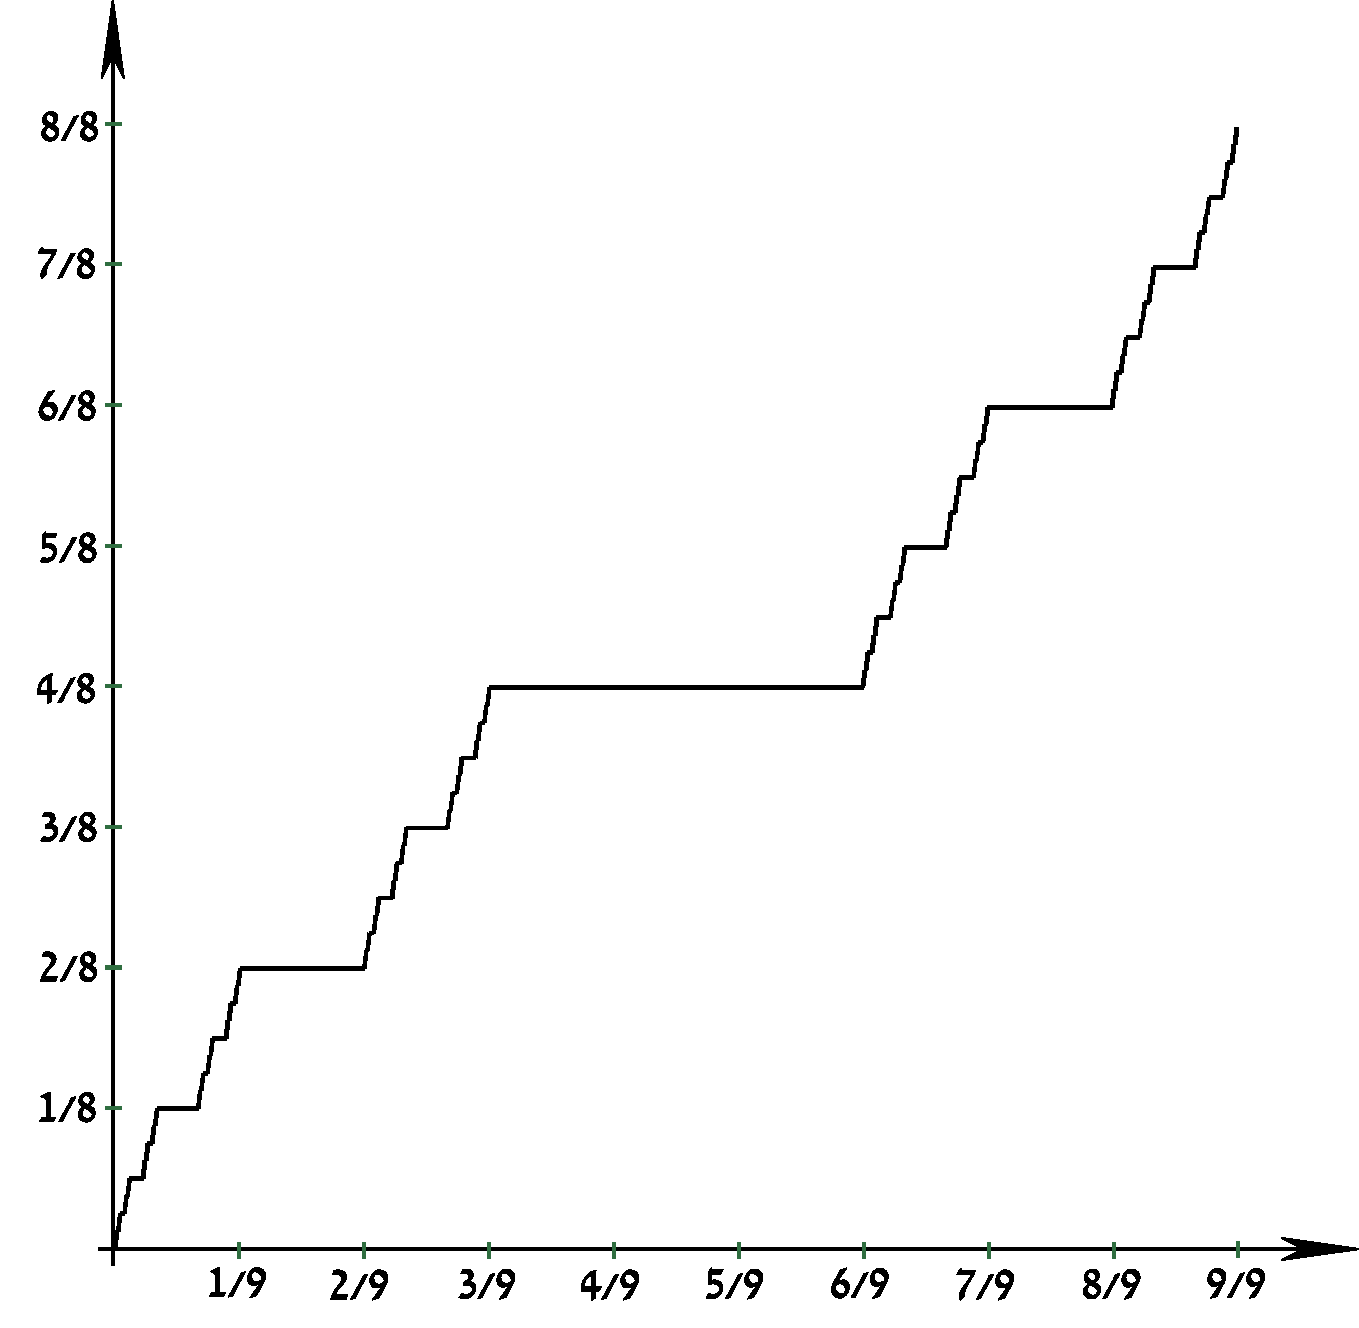
\includegraphics[width=6cm]{attachment/CantorEscalier-2.pdf}
	\caption{Cantor函数在$[0,1]$的图像, “魔鬼阶梯”}
\end{figure}

\circled{A2}-1~~验证Cantor函数在$[0,1]$上连续, 在且仅在$\mathcal{C}$以外可微, 且导数值为$0$. 

\circled{A2}-2~~称一个函数$f$在$[a,b]$上是\textit{绝对连续的}, 如果对任意$\varepsilon >0$存在$\delta >0$使得有限个不交的开区间$(a_k,b_k)$只要满足$\sum_k (b_k-a_k) <\delta$就有$\sum_k |f(b_k)-f(a_k)|<\varepsilon$.\footnote{如果将Newton-Leibniz公式中的Riemann积分替换为Lebesgue积分, 则一个函数符合该公式当且仅当其绝对连续. } 验证Cantor函数在$[0,1]$上并非绝对连续. 

\circled{A2}-3~~求$\int_0^1 c(x) \dif x$. 
\vspace{1em}

\subsection*{B: 积分相关问题}

\circled{B1}-1~~证明: 若$f \in C([a,b])$, 在$[a,b]$上非负, 则$\displaystyle \lim_{n\to \infty} \left( \int_a^b (f(x))^n \dif x \right)^{\frac{1}{n}} = \max_{a \leq x \leq b} f(x).$

\circled{B1}-2~~若$f,\varphi \in C([a,b])$在$[a,b]$上非负, 则$\displaystyle \lim_{n\to \infty} \left( \int_a^b \varphi (x) (f(x))^n \dif x \right)^{\frac{1}{n}} = \max_{a \leq x \leq b} f(x).$

\circled{B1}-3~~若$f \in C([a,b])$, 在$[a,b]$上非负, 证明: $$\lim_{n\to \infty} \left( \left( \int_a^b (f(x))^{n+1} \dif x \right) / \left( \int_a^b (f(x))^n \dif x \right) \right) = \max_{a \leq x \leq b} f(x).$$

将离散的不等式推广: 
\vspace{1em}

\circled{B2}-1~~(Jensen不等式) 设$f,g \in C(\R)$, 且$f$是凸函数, 则当$c \neq 0$时$$f\left( \frac{1}{c} \int_0^c \varphi (t) \dif t \right) \leq \frac{1}{c} \int_0^c f(\varphi (t)) \dif t.$$

\circled{B2}-2~~(Young不等式) 设实数$a,b>0$, 函数$f$在$[a,+\infty )$上连续且严格单调递增, $f(0)=0$, 则$$ab \leq \int_0^a f(x) \dif x + \int_0^b f^{-1}(x) \dif x \leq bf^{-1}(b) + af(a)-f(a)f^{-1}(b),\qquad \textit{取等} \Leftrightarrow f(a)=b.$$

\circled{B2}-3~~(Hölder不等式) 设$\frac{1}{p}+\frac{1}{q}=1$, $f,g$在$[a,b]$上Riemann可积. 则当$p > 1$时有$$\left| \int_a^b f(x)g(x) \dif x \right|\leq \left( \int_a^b |f(x)|^p \dif x \right)^{\frac{1}{p}} \left( \int_a^b |g(x)|^q \dif x \right)^{\frac{1}{q}}  ,\qquad \textit{取等}\Leftrightarrow |f|^p=\lambda |g|^q. $$
当$0<p<1$时上述不等式反向. 取$p=q=2$, 即得Cauchy-Schwarz不等式. 
\vspace{1em}

\circled{B2}-4~~(Minkowski不等式) 设$f,g$在$[a,b]$上Riemann可积. 当$p \geq 1$时有$$\left| \int_a^b |f(x)+g(x)|^p \dif x \right|^{\frac{1}{p}} \leq \left( \int_a^b |f(x)|^p \dif x \right)^{\frac{1}{p}} + \left( \int_a^b |g(x)|^q \dif x \right)^{\frac{1}{q}},\qquad \textit{取等}\Leftrightarrow |f|^p=\lambda |g|^q.$$
当$0<p<1$时上述不等式反向. 




\newpage
\section*{一些习题 ~~\small 对应原书6.3习题} \label{sec:ex7.2}

\newpage
\section{有向可加函数与Stieltjes积分}

将Riemann积分算子的区间可加性抽象出来, 得到所谓可加函数. 即, 设$I:U \times U \to V$, 若对任意$x,y,z \in U$都有$I(x,z)=I(x,y)+I(y,z)$, 则称$I$为$U$上的\textit{有向可加函数}. 这里用一般的$U,V$是为了强调有向可加函数的性质与$\R$的特殊结构无关. 

实际上, 除了Riemann积分以外, 很多函数都是有向可加函数. 例如, 相对速度的计算公式$v_{13}=v_{12}+v_{23}$, 电势差$\varphi _{ac}=\varphi _{ab}+\varphi _{bc}$等等. 不难发现, 电势差$\varphi _{ab}$的背后是场强的(多元函数)积分$\int_a^b E(r) \dif r$, 但是相对速度背后并没有明显的积分背景. 这一现象提示我们研究, 何种有向可加函数能表示为Riemann积分? 更进一步, 注意到有些离散情况的公式和积分公式非常相似(如Abel变换和分部积分), 那么可否发展一种积分理论将这些公式统一起来? 

在第一小节, 我们会探讨哪些函数能表示为Riemann积分(毕竟这种积分易于计算)及其计算. 而作为推广的Stieltjes积分将在第二小节介绍. 

\subsection{有向可加函数的Riemann积分表示}

下面的命题给出积分产生有向可加函数的一个充分条件. 

\begin{proposition}{}
	设有向可加函数$I:[a,b] \times [a,b] \to \R$. 若存在$f \in \mathcal{R}([a,b])$使得对任意$a \leq \alpha < \beta \leq b$都有$$\inf_{x\in [\alpha ,\beta]} f(x) (\beta -\alpha) \leq I(\alpha ,\beta) \leq \sup_{x\in [\alpha ,\beta]} f(x) (\beta -\alpha),$$
	则$\displaystyle I(a,b)=\int_a^b f(x) \dif x$. 
\end{proposition}

\subsection{Stieltjes积分}

对于有向可加函数$I:[a,b] \times [a,b] \to \R$, 通过定义函数$\mu :[a,b] \to \R ,t \mapsto I(a,t)$, 可将$I(\alpha ,\beta)$视作$\mu (\beta)-\mu (\alpha)$. 从几何的视角, 若将$I(\alpha ,\beta)$视作区间$[\alpha ,\beta ]$的长度(两端点的有向距离), 则$\mu$就给出了某个点的绝对位置(亦称$\mu$为测度函数). Riemann积分即是$\mu (x)=x$的情形. 这启发我们, 将Riemann积分中的$\dif x$替换为$\dif \mu (x)$, 或者说将Riemann和中的$x_i-x_{i-1}$替换为$\mu (x_i)- \mu (x_{i-1})$. 

需要注意的是, 虽然$\mu $的单调性不影响Stieltjes积分的定义, 但一般为了保证其良好性质, 会约定$\mu$不减. 

\begin{definition}{Stieltjes积分}
	设闭区间$I$上的函数$f$和不减的函数$\mu$, 定义
	\begin{itemize}
		\item 对于分划$\pi = \{ a=x_0<\cdots <x_n=b \}$, 称形如$$f = \sum_{i=1}^{n} \lambda _i \chi _{(\mu (x_{i-1}),\mu (x_{i}))} $$
		(其中$\lambda _i \in \R$)的函数为$\pi$上的一个\textit{$\mu$-阶梯函数}. 记$I$上全体$\mu$-阶梯函数的集合为$\mathcal{S}(I;\mu )$. 
		\item 承上一条, 定义$f$的\textit{积分}(integral)为$$\int f := \sum_{i=1}^{n} \lambda _i \int \chi _{(\mu (x_{i-1}), \mu (x_i))} = \sum_{i=1}^{n} \lambda _i (\mu (x_i)-\mu (x_{i-1})). $$
		\item 称$f$是\textit{Stieltjes可积的}, 如果对任意$\varepsilon >0$均存在$F,e \in \mathcal{S}(I;\mu )$使得$$\forall x \in I,|f(x)-F(x)|<e(x),\qquad \int e < \varepsilon .$$
	全体$I$上Riemann可积的函数构成集合$\mathcal{R}(I;\mu)$. 
	\end{itemize}
	类似Riemann积分, 我们还能验证Riemann和的定义与上方定义等价: 
	\begin{itemize}
		\item $f$的\textit{Riemann和}为$$S(f;\pi ,\xi) := \sum_{i=1}^{n} (\mu(x_i)-\mu(x_{i-1}))f(\xi _i) .$$
		\item 固定$f$, 它的\textit{基}为$\mathcal{B} := \{ B_{\delta}:\delta >0 \}$, 其中$B_{\delta} := \{ (\pi ,\xi) : \| \pi \|< \delta \}$. 
		\item 称$f$在$I$上\textit{Stieltjes可积}, 若极限$\displaystyle \lim_{\mathcal{B}} S(f;\pi ,\xi)$存在, 且将其定义为$\displaystyle \int_a^b f(x) \dif \mu (x)$. 
	\end{itemize}
\end{definition}

同样地, 对阶梯函数与Riemann和而言, 分别可以定义上下积分及Darboux上下和. 这里省略具体定义. 

可以证明Stieltjes积分拥有和Riemann积分类似的性质, 即命题\ref{pro:jiffxkvi1}, \ref{pro:kejiisyc}(要将$x$换成$\mu (x)$), \ref{pro:jiffxkvi}. 

类似于换元积分公式, 不难证明, 设$\mu (x) = \int_a^x \rho (x)\dif x$, 则对可积的$f$有$\displaystyle \int_a^b f(x) \dif \mu (x) = \int_a^b f(x) \rho (x) \dif x$. 特别地, 当$\mu$连续可微时, 就可以将积分号内的$\dif \mu (x)$看做是$\mu '(x) \dif x$. 

然而, 唯一与Riemann积分不同之处在于, Stieltjes积分没有Newton-Leibniz公式. 这是否意味着其没有作为Newton-Leibniz公式推论的分部积分公式? 实际上, 用Abel求和来逼近, 可以证明类似分部积分公式而将Riemann积分与Stieltjes积分联系起来的公式. 

\begin{proposition}{Riemann积分与Stieltjes积分的联系}
	设不减函数$\mu$, $f \in C^1([a,b])$, 则$$\int_a^b f'(x)\mu (x) \dif x = f(x)\mu (x) \mid _a^b - \int_a^b f(x) \dif \mu (x) .$$
\end{proposition}















\chapter{多元函数微分学}

\section{导数与微分}

\subsection{基本定义}

我们总是假设$\Omega$是$\R ^n$中的开集. 

\begin{definition}{方向导数, 偏导数}
    设函数$f:\Omega \to \R$, $x_0 \in \Omega , v \in \R ^n$. 定义$f$在$x_0$处\textit{沿$v$的方向导数}为下列极限(如果存在): $$\frac{\p f}{\p v}(x_0) := \lim_{h \to 0} \frac{f(x_0+hv)-f(x_0)}{h}.$$
    特别地, 令$\frac{\p }{\p x_i}$表示第$i$个坐标为$1$, 其余为$0$的单位向量, 则称沿$x_i$的方向导数为该方向上的\textit{偏导数}. 
\end{definition}

从几何的视角理解方向导数: 设曲线$\gamma :(-\delta,\delta) \to \R ^n$是$C^1$的. 我们有$$\frac{\dif}{\dif t} \big|_{t=0} (f|_{\rge \gamma} \circ \gamma) = \frac{\p f}{\p \gamma '(0)} (\gamma (0)). $$



\subsection{导数与微分的计算}

\subsection{$\R ^n$中的子流形}

\newpage
\section{中值定理与Taylor公式}

\subsection{微分中值定理}

\subsection{Taylor公式}

\subsection{多元函数的极值}

\newpage
\section{隐函数定理}

\subsection{反函数定理}

\subsection{隐函数定理}


\newpage
\section{隐函数定理的应用}

\subsection{流形版本的隐函数定理}

\subsection{Lagrange乘子法}
\chapter{微分学的一般化}



\backmatter
\chapter*{习题参考解答}

% Appendices section.
% \appendix

% Include the "about" appendix from the BackMatter subfolder.
% \chapter{About the Authors}

\section{First Author}

\blindtext

\section{Second Author}

\blindtext

% Include the "abbreviation" appendix from the BackMatter subfolder.
% \chapter{Abbreviations}

\blindtext

% Include the "notation" appendix from the BackMatter subfolder.
% \chapter{Notation}

\blindtext

% Include the "code" appendix from the BackMatter subfolder.
% \chapter{Supplementary Scripts}

\blindtext

% Include the "glossary" appendix from the BackMatter subfolder.
% \chapter{Glossary}

\blindtext

% Include the "index" appendix from the BackMatter subfolder.
% \chapter{Index}

\blindtext

% Include the "references" appendix from the BackMatter subfolder.
% \bibliography{references.bib}
\bibliographystyle{ieeetr}
\nocite{*}

% End the document.


\end{document}
